\documentclass[12pt,letterpaper,twoside]{report}
\usepackage[utf8]{inputenc}
\usepackage{amsmath}
\usepackage{amsfonts}
\usepackage{amssymb}
\usepackage[margin=0.75in]{geometry}
\usepackage{array}
\usepackage{tabu}
\usepackage{fancyhdr}
\usepackage{bm}
\usepackage{tocloft}
\usepackage{multirow}
\usepackage{subcaption}
\usepackage{float}
\usepackage[export]{adjustbox}
\usepackage{url}
\usepackage{wrapfig}
\usepackage{ulem}

\usepackage [english]{babel}
\usepackage [autostyle, english = american]{csquotes}
\MakeOuterQuote{"}

\author{Elizabeth Croft, Agnes d'Entremont \\  \\ Department of Mechanical Engineering \\ The University of British Columbia}

\pagestyle{fancy}
\fancyhf{}
\fancyhead[LE,RO]{UBC}
\fancyhead[RE,LO]{MECH 221 Dynamics Notes}
\fancyfoot[CE,CO]{Chapter \thechapter}
\fancyfoot[LE,RO]{\thepage}
\fancyfoot[RE,LO]{CC BY-SA E. Croft/A. d'Entremont}

\renewcommand{\headrulewidth}{2pt}
\renewcommand{\footrulewidth}{1pt}

\setlength{\parindent}{0em}
\setlength{\parskip}{1em}
\renewcommand{\baselinestretch}{1.0}

% Redefine the plain page style
\fancypagestyle{plain}{%
  \fancyhf{}%
  \fancyhead[LE,RO]{UBC}
  \fancyhead[RE,LO]{MECH 221 Dynamics Notes}
  \fancyfoot[CE,CO]{Chapter \thechapter}
  \fancyfoot[LE,RO]{\thepage}
  \fancyfoot[RE,LO]{CC BY-SA E. Croft/A. d'Entremont}
  \renewcommand{\headrulewidth}{2pt}% Line at the header invisible
  \renewcommand{\footrulewidth}{1pt}% Line at the footer visible
}



\usepackage{titlesec}
\titleformat{\chapter}
  {\normalfont\Large\bfseries}{\thechapter}{1em}{}
\titlespacing*{\chapter}{0pt}{3.5ex plus 1ex minus .2ex}{2.3ex plus .2ex}
\titleformat{\section}
  {\normalfont\large\bfseries}{\thesection}{1em}{}
\titlespacing*{\section}{0pt}{8pt}{2pt}


\setlength\cftparskip{-2pt} 
\setlength\cftbeforechapskip{2pt}

\usepackage{graphicx}
\graphicspath{ {./MECH221_DYN_notes_images/}}



\begin{document}

\title{MECH 221 Dynamics Notes}
\date{Fall 2020}
\maketitle

\chapter*{Preface}
\addcontentsline{toc}{chapter}{Preface}
These notes were authored by Dr. Elizabeth Croft (currently at Monash University, \url{elizabeth.croft@monash.edu}) in 2004, and converted for open licensing (including figure creation) in 2019 by Dr. Agnes d'Entremont (\url{adentremont@mech.ubc.ca}) from the Department of Mechanical Engineering at the University of British Columbia, Vancouver, Canada (\url{https://mech.ubc.ca}).  

The notes are designed to be used for a second-year dynamics course in Mechanical Engineering, and cover planar rigid-body dynamics and an introduction to one degree-of-freedom vibrations. The order of topics has vibrations earlier in the series than typical, due to their use in an integrated course. This order matches the course timing of related ordinary differential equation solutions in the integrated mathematics and electric circuits courses. 

These notes are intended to be skeleton notes, with substantial portions (diagrams, derivations, solutions) written in by students along with their instructor.  Completed notes are available to instructors.  

This work is licensed under a Creative Commons Attribution-ShareAlike 4.0 International License. 

\newpage
\tableofcontents

\chapter{L1: Rigid Body Kinematics - Chasles' Theorem}
Readings

\section{Objective}
To describe the planar motion of a rigid body.

\section{Introduction: Chasles’ Theorem}
The motion of rigid body can be described by the \textbf{translation} of \textbf{\textit{one point}} plus the \textbf{rotation} about that same point.


\vspace*{10\baselineskip}

\begin{center}
\begin{tabu} to 1\textwidth {  X[c]  X[c] X[c] X[c]  X[c]  }
$\bm{v_A}$ & $+$ & $\bm{\omega} \times \bm{r_{B/A}}$ & $=$ & $\bm{v_B}$\\
 & & & & \\
Translational velocity at $A$ & $+$ & Velocity due to rotation of point $B$ about $A$ & $=$ & Velocity at point $B$\\

\end{tabu}
\end{center}

\textbf{IMPORTANT NOTE:} For a RIGID BODY, angular velocity is the SAME at all points on the body. 


\section{Types of Rigid Body Motion}

\begin{center}
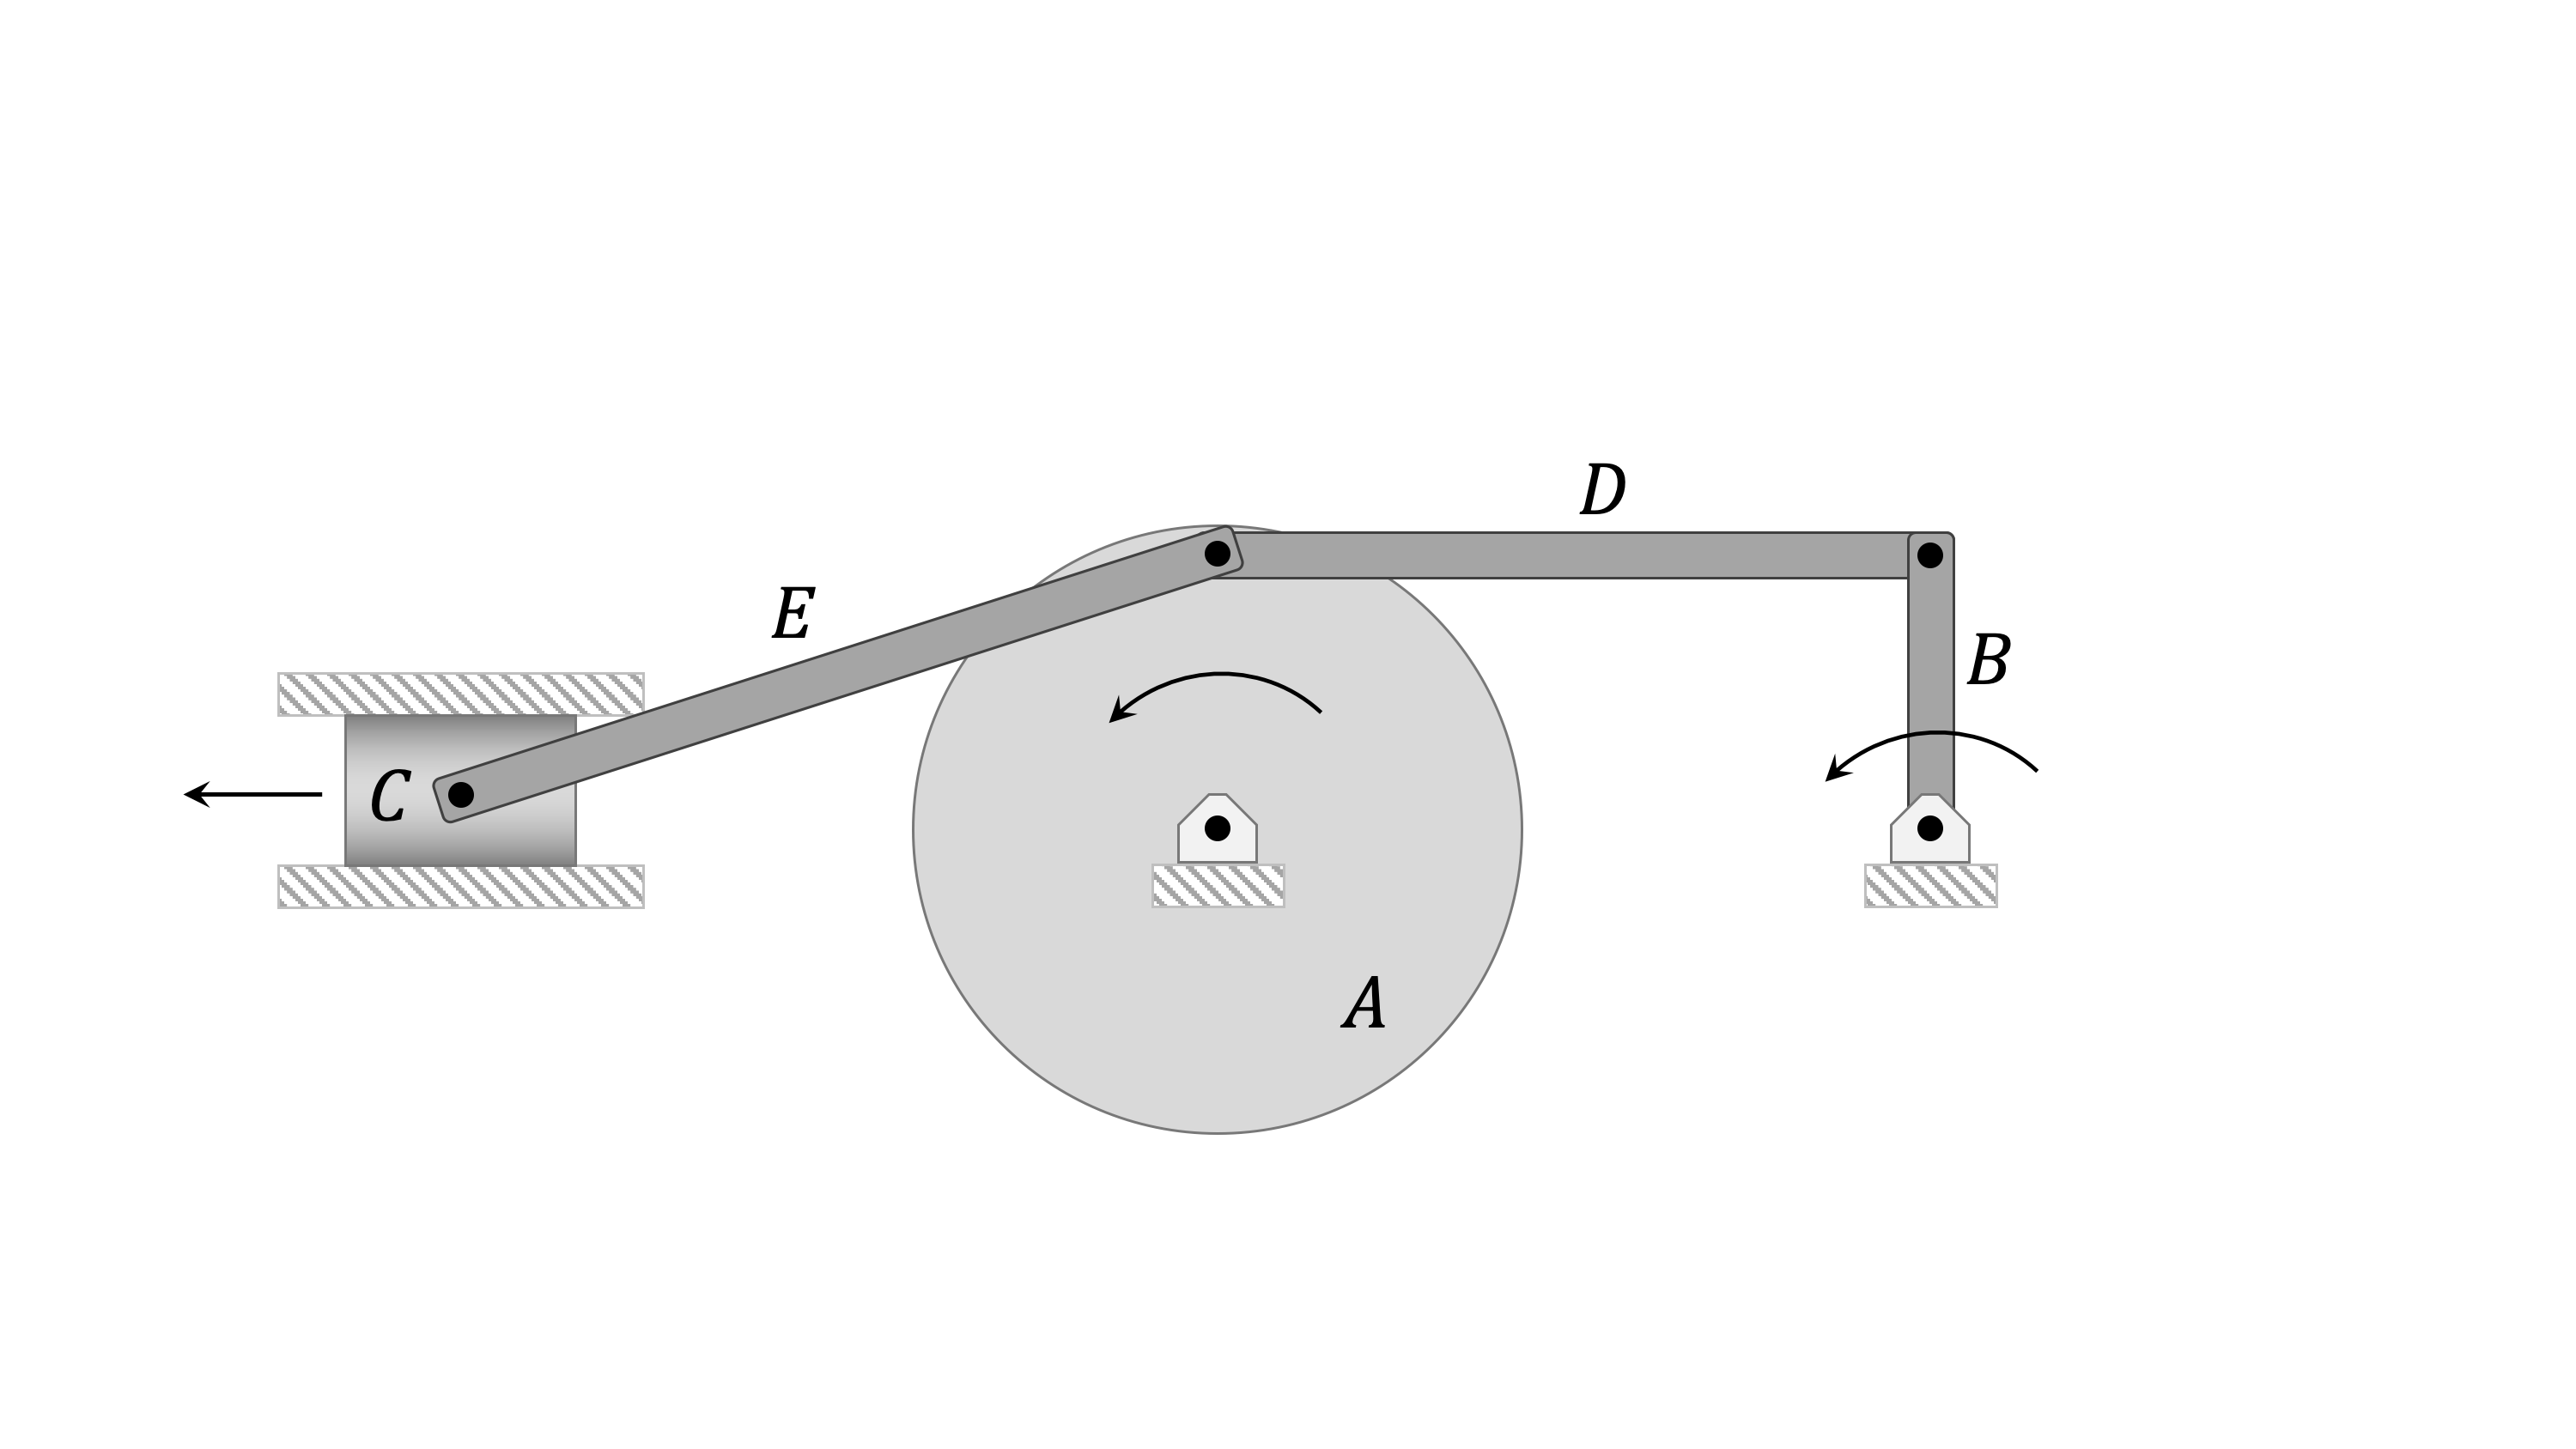
\includegraphics[trim={2cm 4cm 5cm 5.5cm},clip,width=0.75\textwidth]{Slide2}
\end{center}

% trim={<left> <lower> <right> <upper>}

An example of bodies undergoing the three types of motion is shown in the above mechanism.

The wheel and crank (A and B) undergo \textbf{rotation about a fixed axis}.  In this case, both axes of rotation are at the location of the pins and perpendicular to the plane of the figure.

The piston (C) undergoes \textbf{rectilinear translation} since it is constrained to slide in a straight line.  

The connecting rod (D) undergoes \textbf{curvilinear translation}, since it will remain horizontal as it moves along a circular path.

The connecting rod (E) undergoes \textbf{general plane motion}\textsl{•}


\section{Pure Translation}
If a body is \textbf{translating only}, the motion equations are the same as for particle motion – all points travel at the same velocity, acceleration, etc.

The angular velocity of the body, $\omega = 0$

\begin{figure}[H]
\centering
\begin{subfigure}[b]{0.4\textwidth}
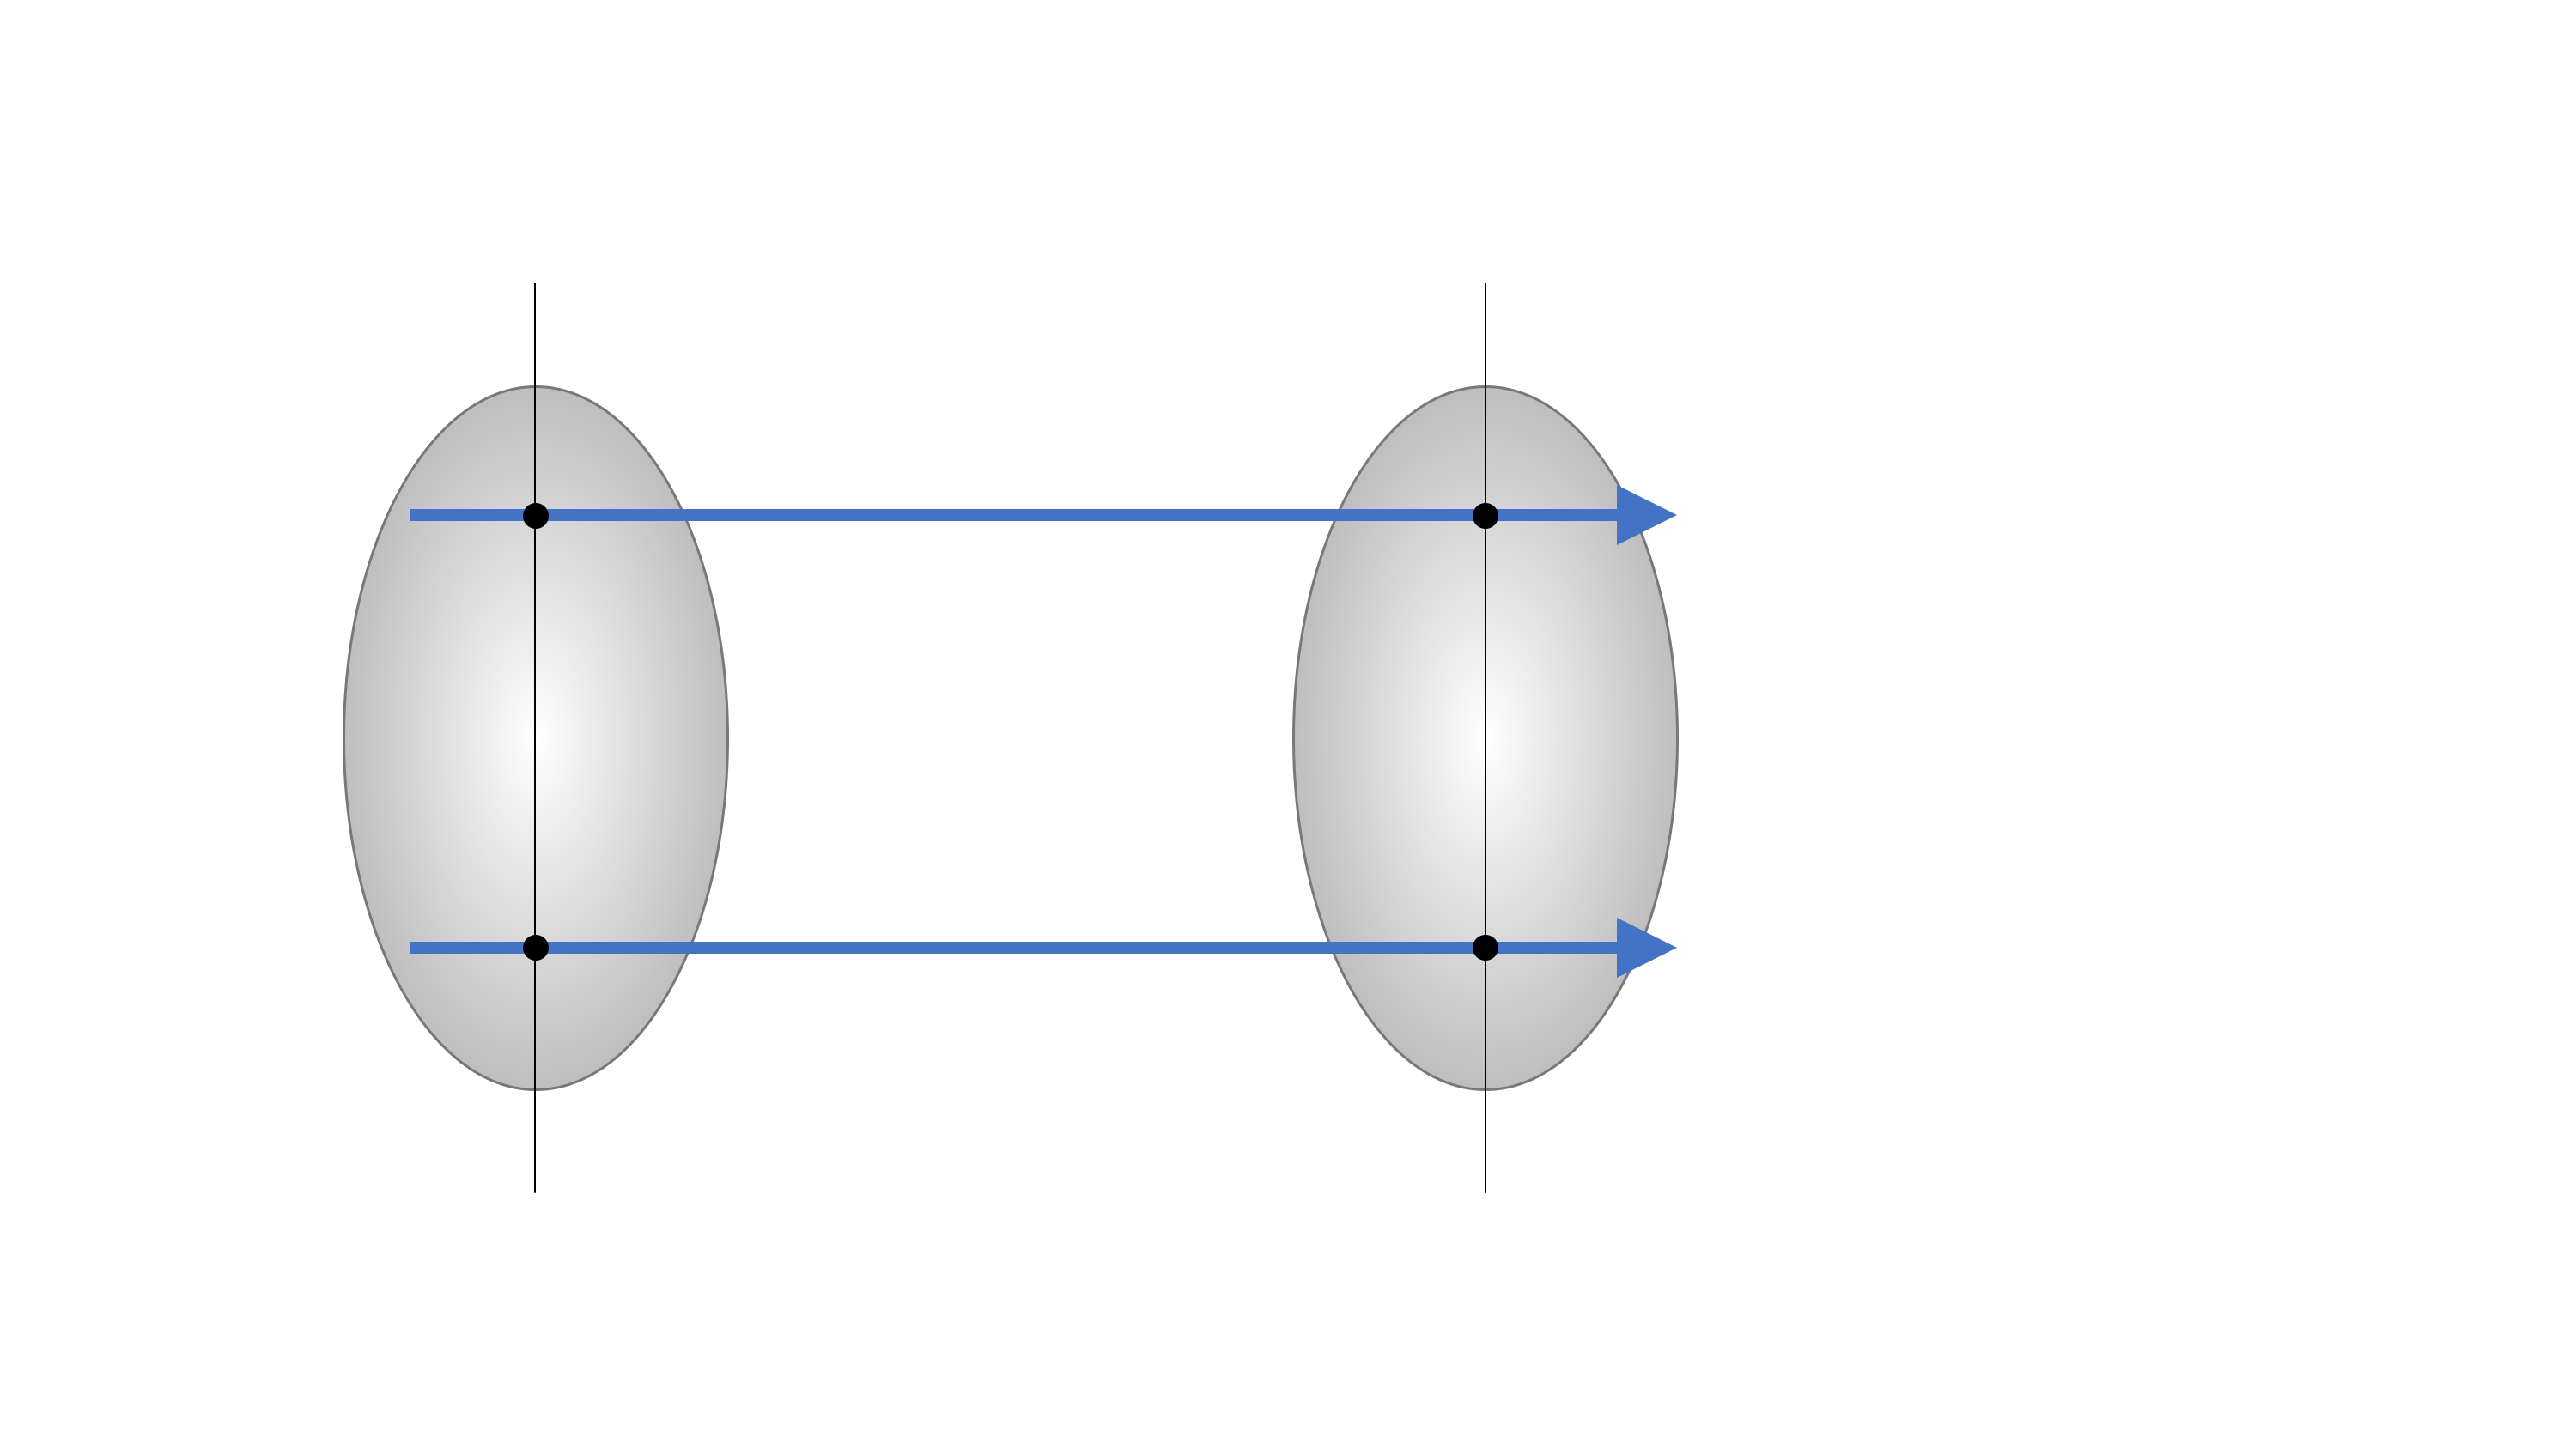
\includegraphics[trim={2cm 2cm 8.5cm 2cm},clip,width=\textwidth]{Slide3}
        \caption{Rectilinear translation}
        \label{fig:Slide3}
    \end{subfigure}
    ~ 
    \begin{subfigure}[b]{0.4\textwidth}
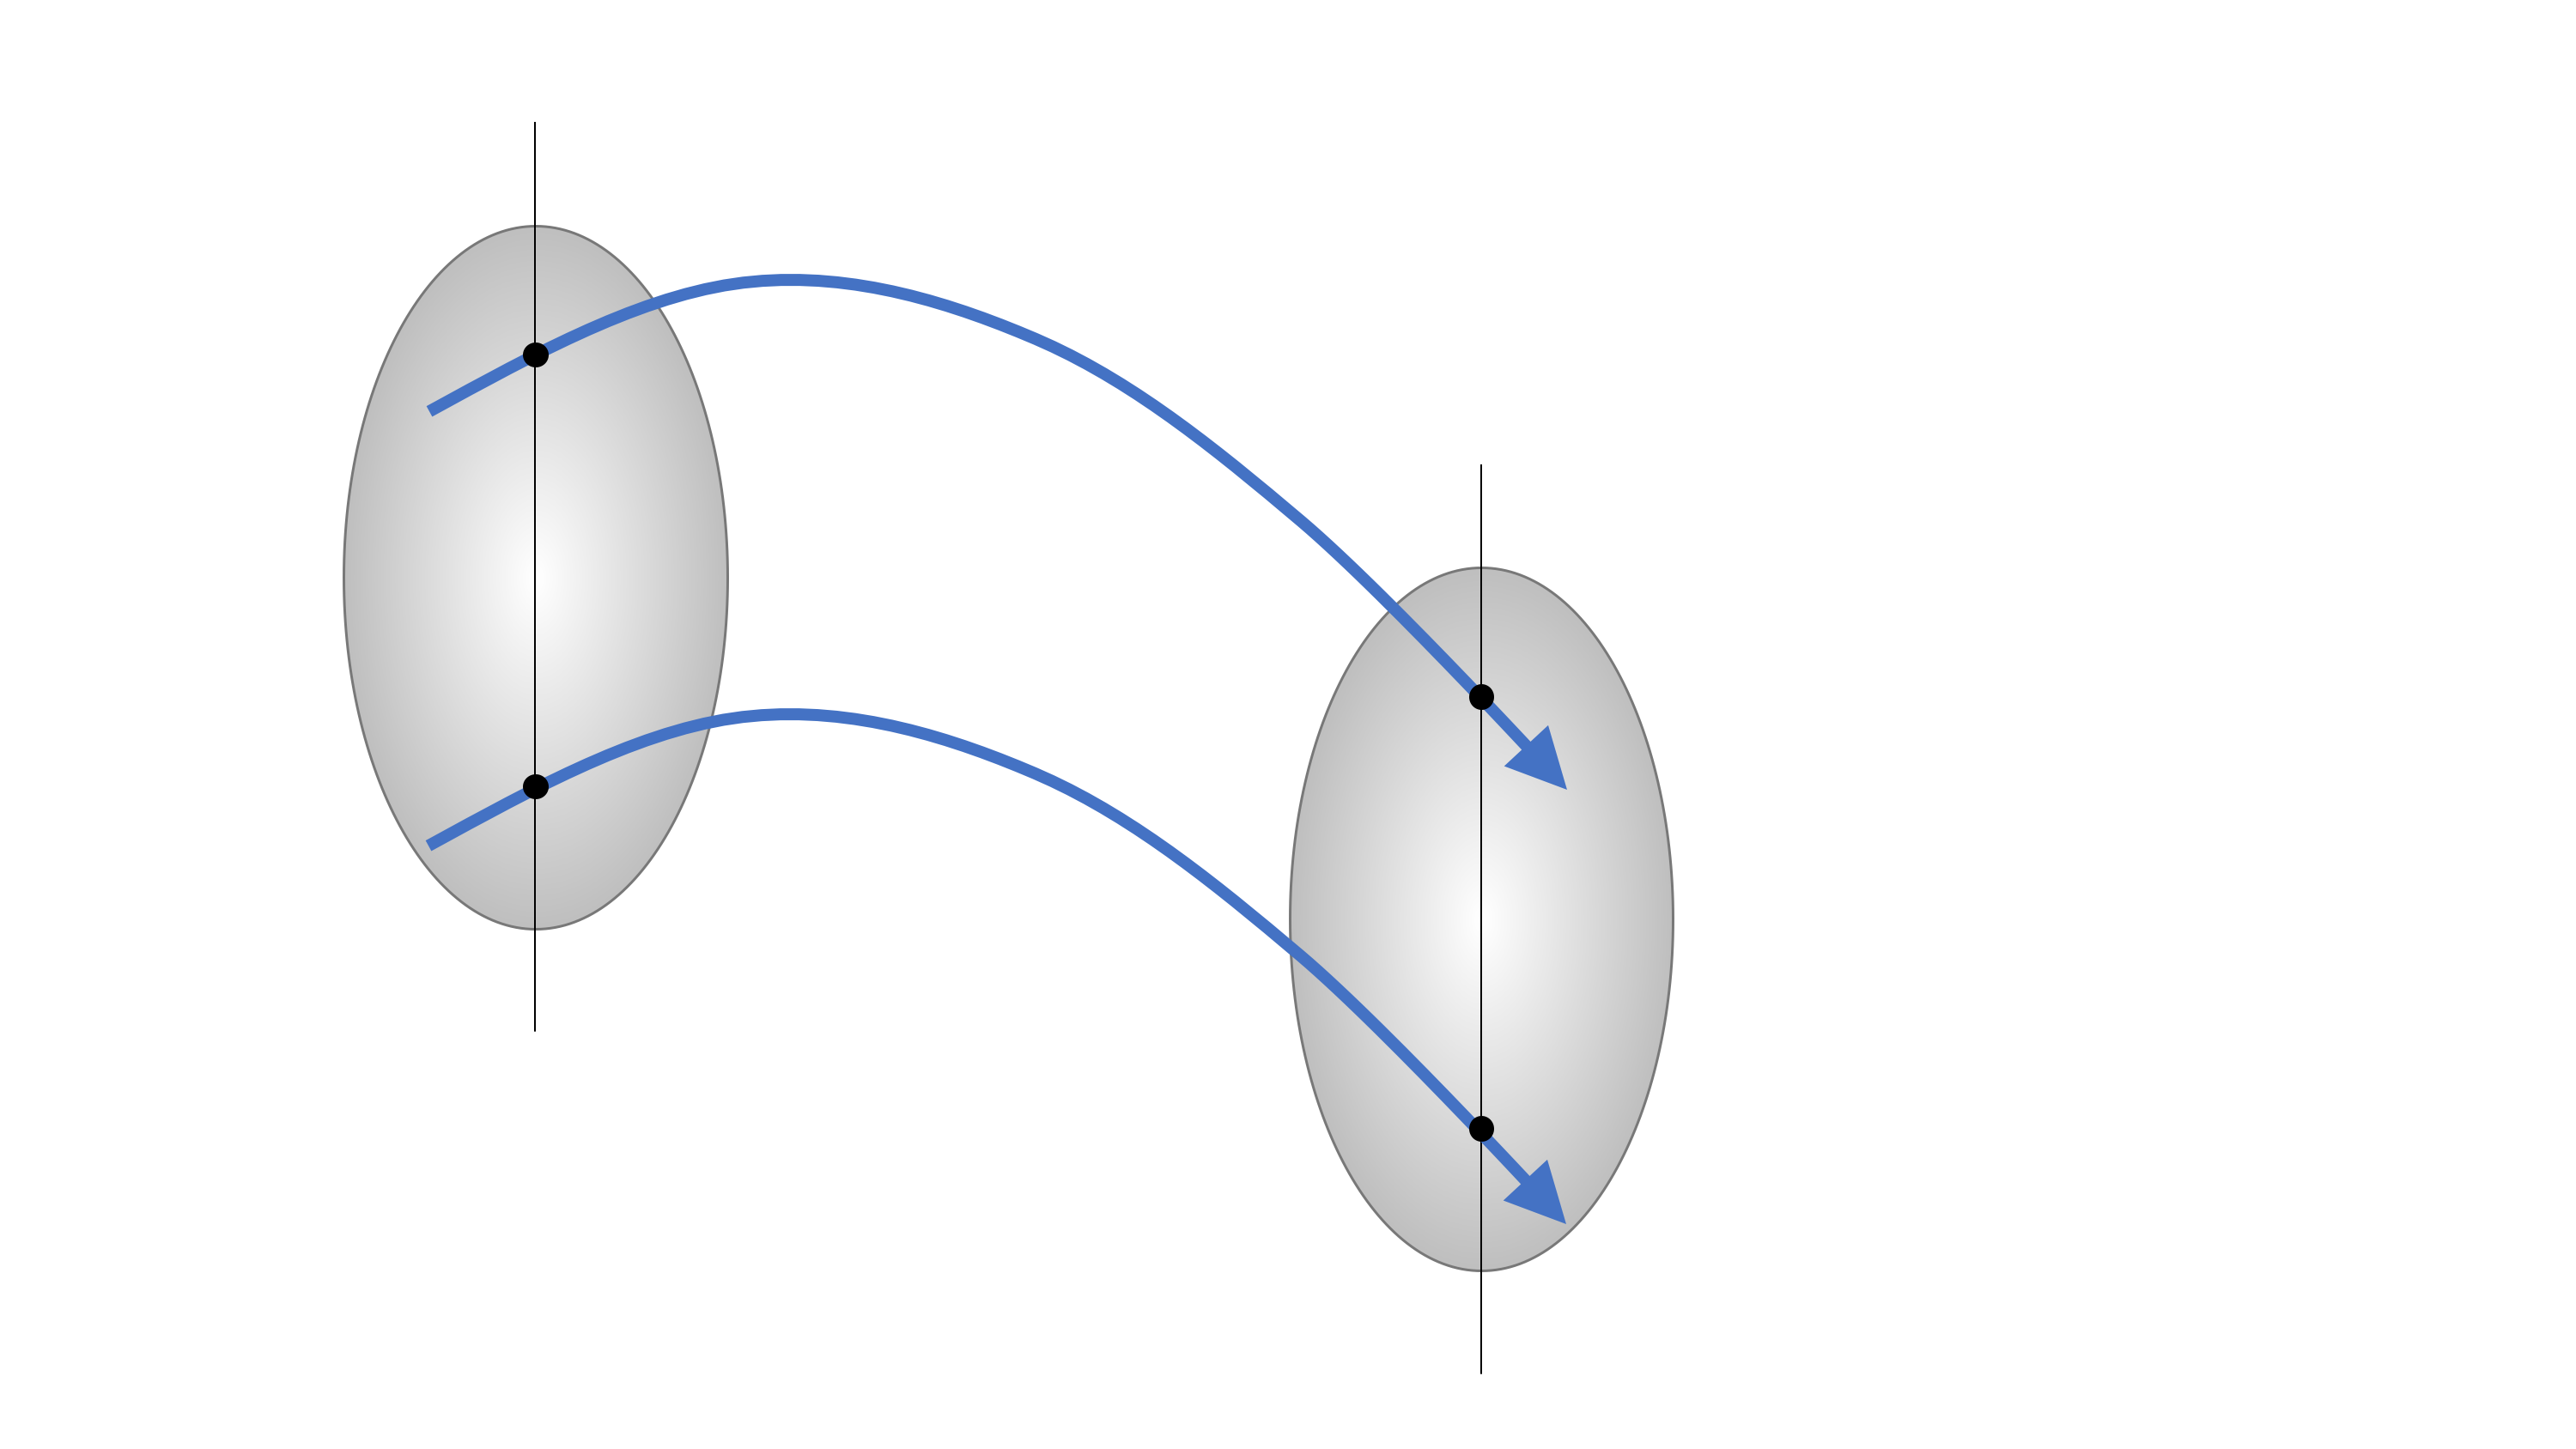
\includegraphics[trim={2cm 1.5cm 8.5cm 2cm},clip,width=\textwidth]{Slide4}
        \caption{Curvilinear translation}
        \label{fig:Slide4}
    \end{subfigure}

\end{figure}


\begin{minipage}[c]{0.3\textwidth}
\begin{tabular}{  c  c }
Position: & $\bm{r_B} = \bm{r_A} + \bm{r_{B/A}}$\\
 &  \\
Velocity: & $\bm{v_B} = \bm{v_A} $\\
 &  \\
Acceleration: & $\bm{a_B} = \bm{a_A} $\\
\end{tabular}
\label{tab:singlebest}
\end{minipage}%%%
\begin{minipage}[c]{0.7\textwidth}
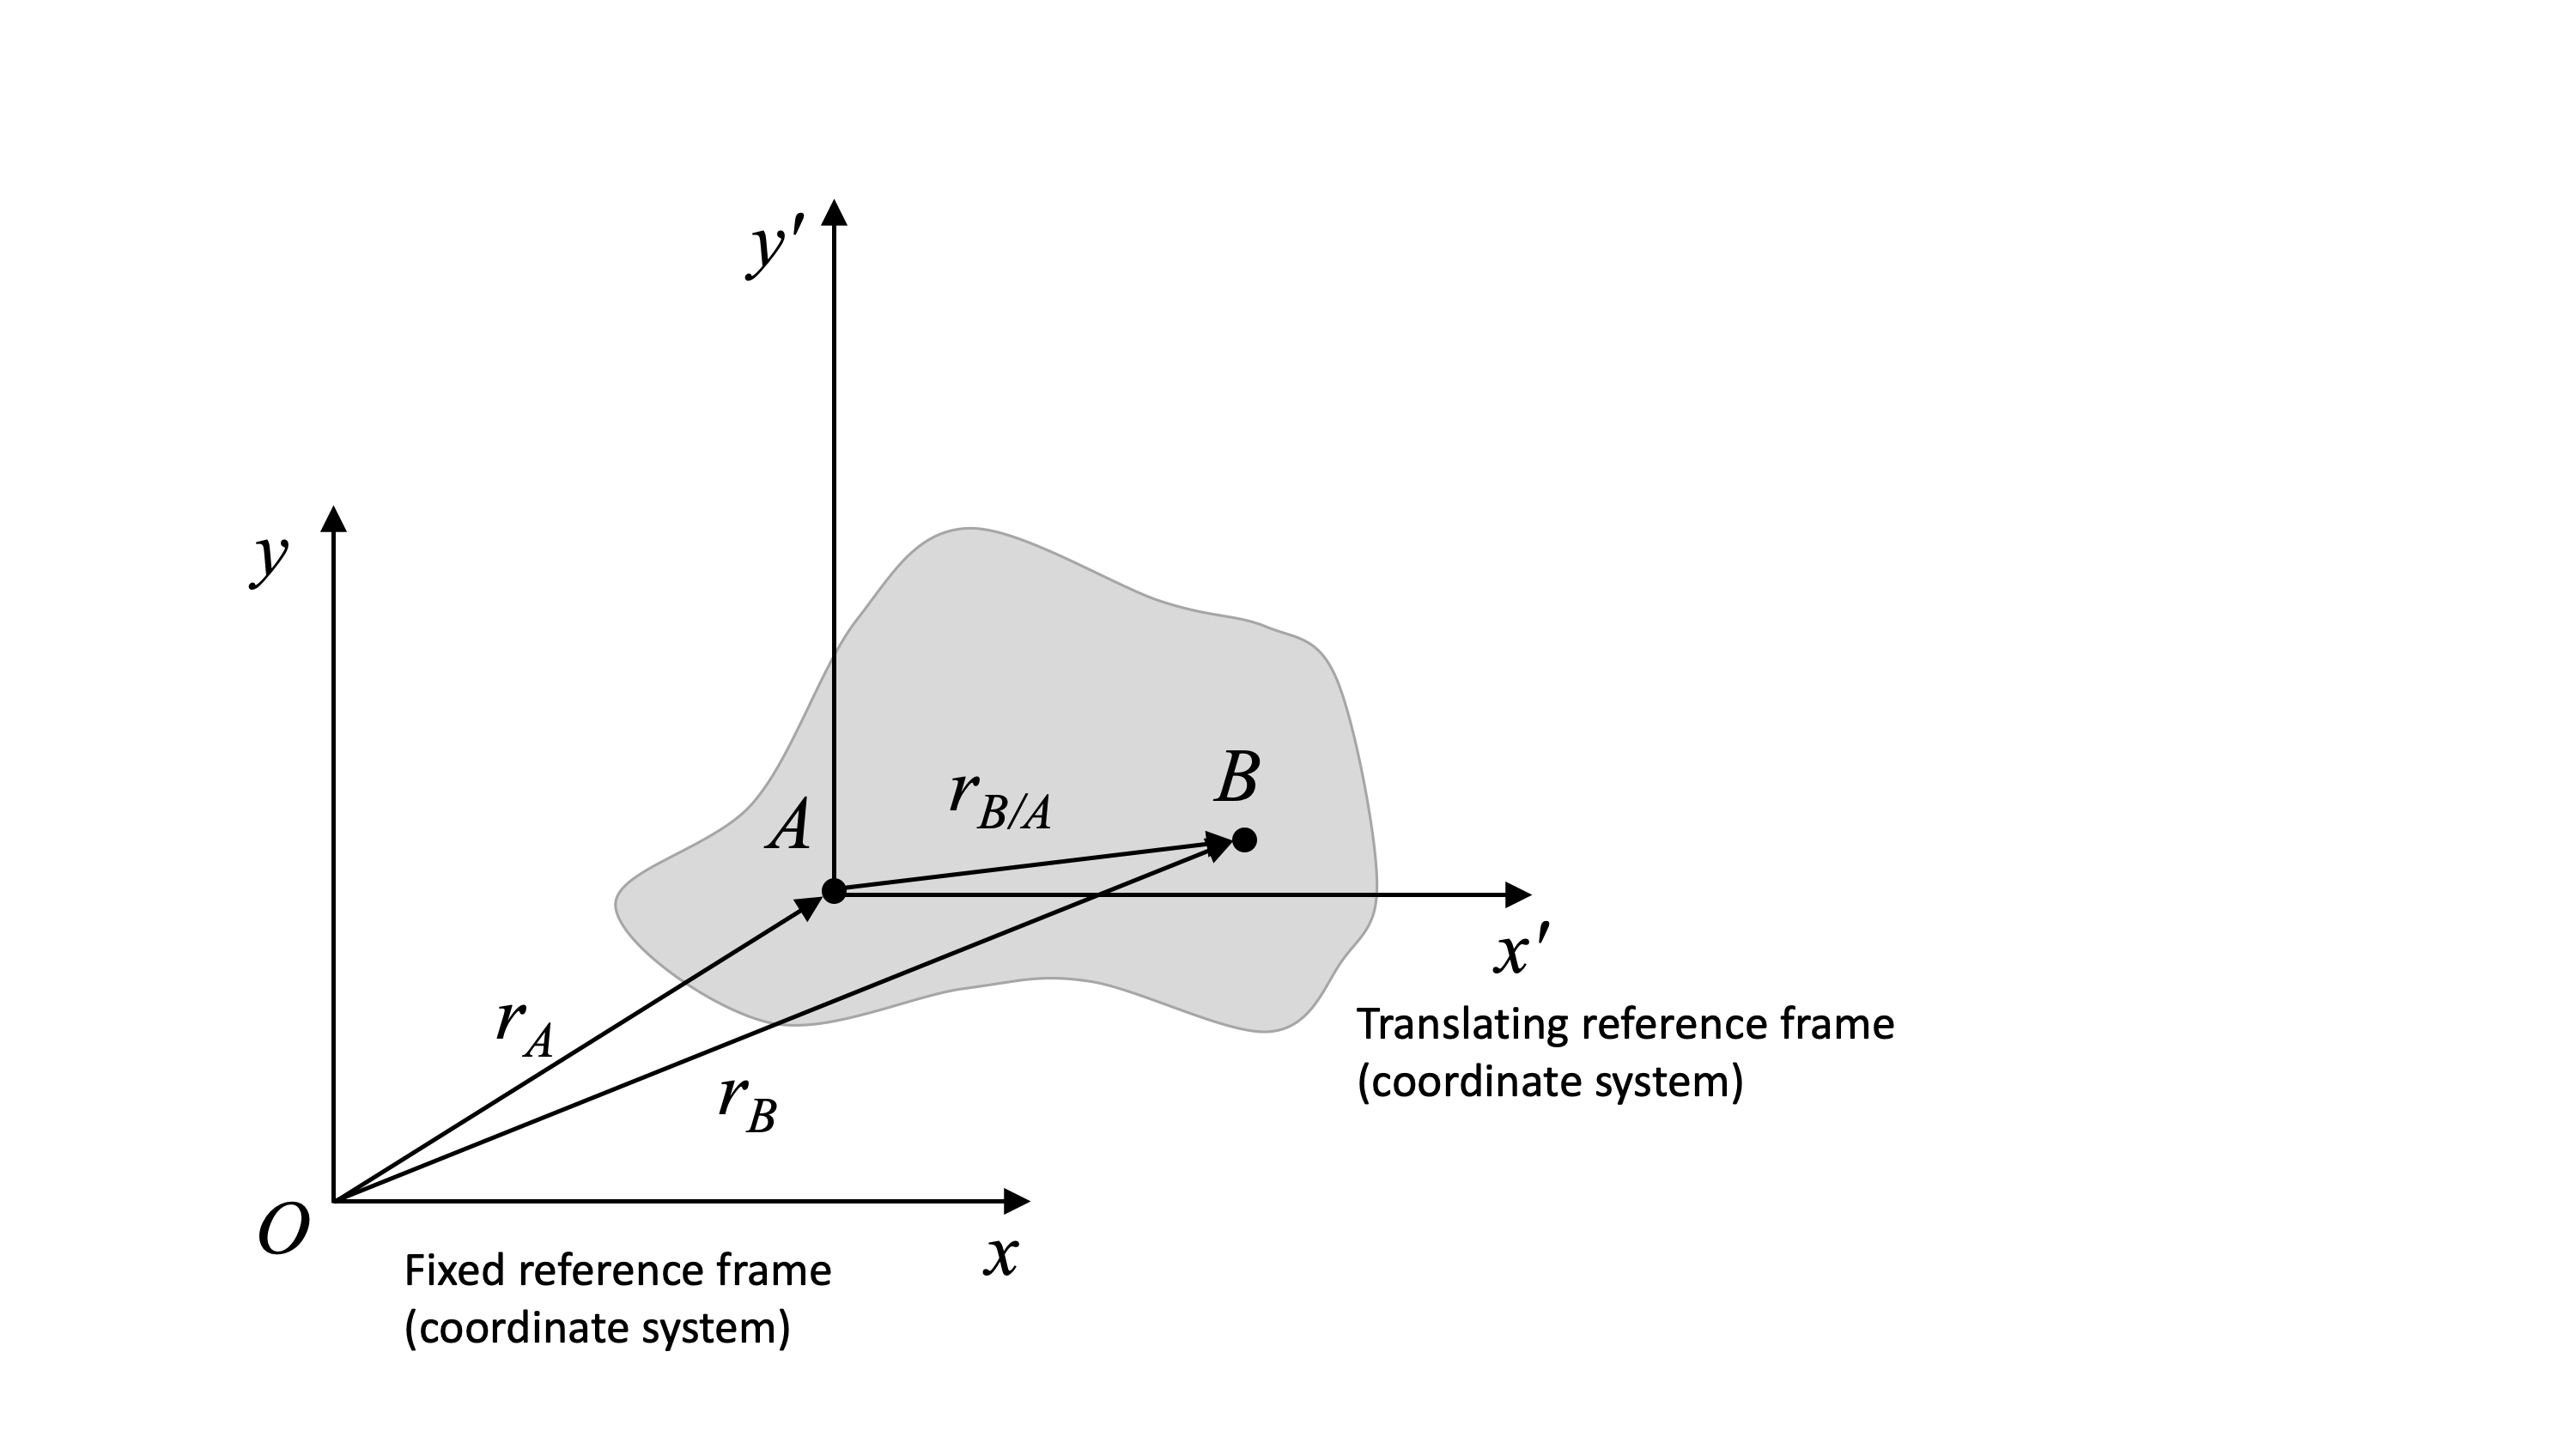
\includegraphics[trim={3cm 0cm 7.5cm 1.5cm},clip,width=0.9\textwidth, right]{Slide5}
\end{minipage}

\section{Pure Rotation}

When a rigid body is \textbf{pinned} it rotates about a fixed point, eg. $P$.  Since $v_P=0$, $a_P=0$, we only need to consider the motion of the rest of the body with respect to point $P$.  

Cranks, rotating shafts and bodies mounted to fixed hinges are all examples of pure rotation systems.  

\subsection{Example}
Consider the crank arm CB.  It has angular velocity $\bm{\omega_{BC}}=1 \, rad/s \, \bm{\hat{k}}$ and angular acceleration $\bm{\alpha_{BC}} =1 \, rad/s^2 \, \bm{\hat{k}}$.  The length of CB is $1 \, m$.  Compute the velocity and acceleration of point $B$ when the crank arm forms an angle $\theta =45^{\circ}$ with the horizontal plane, as shown. 

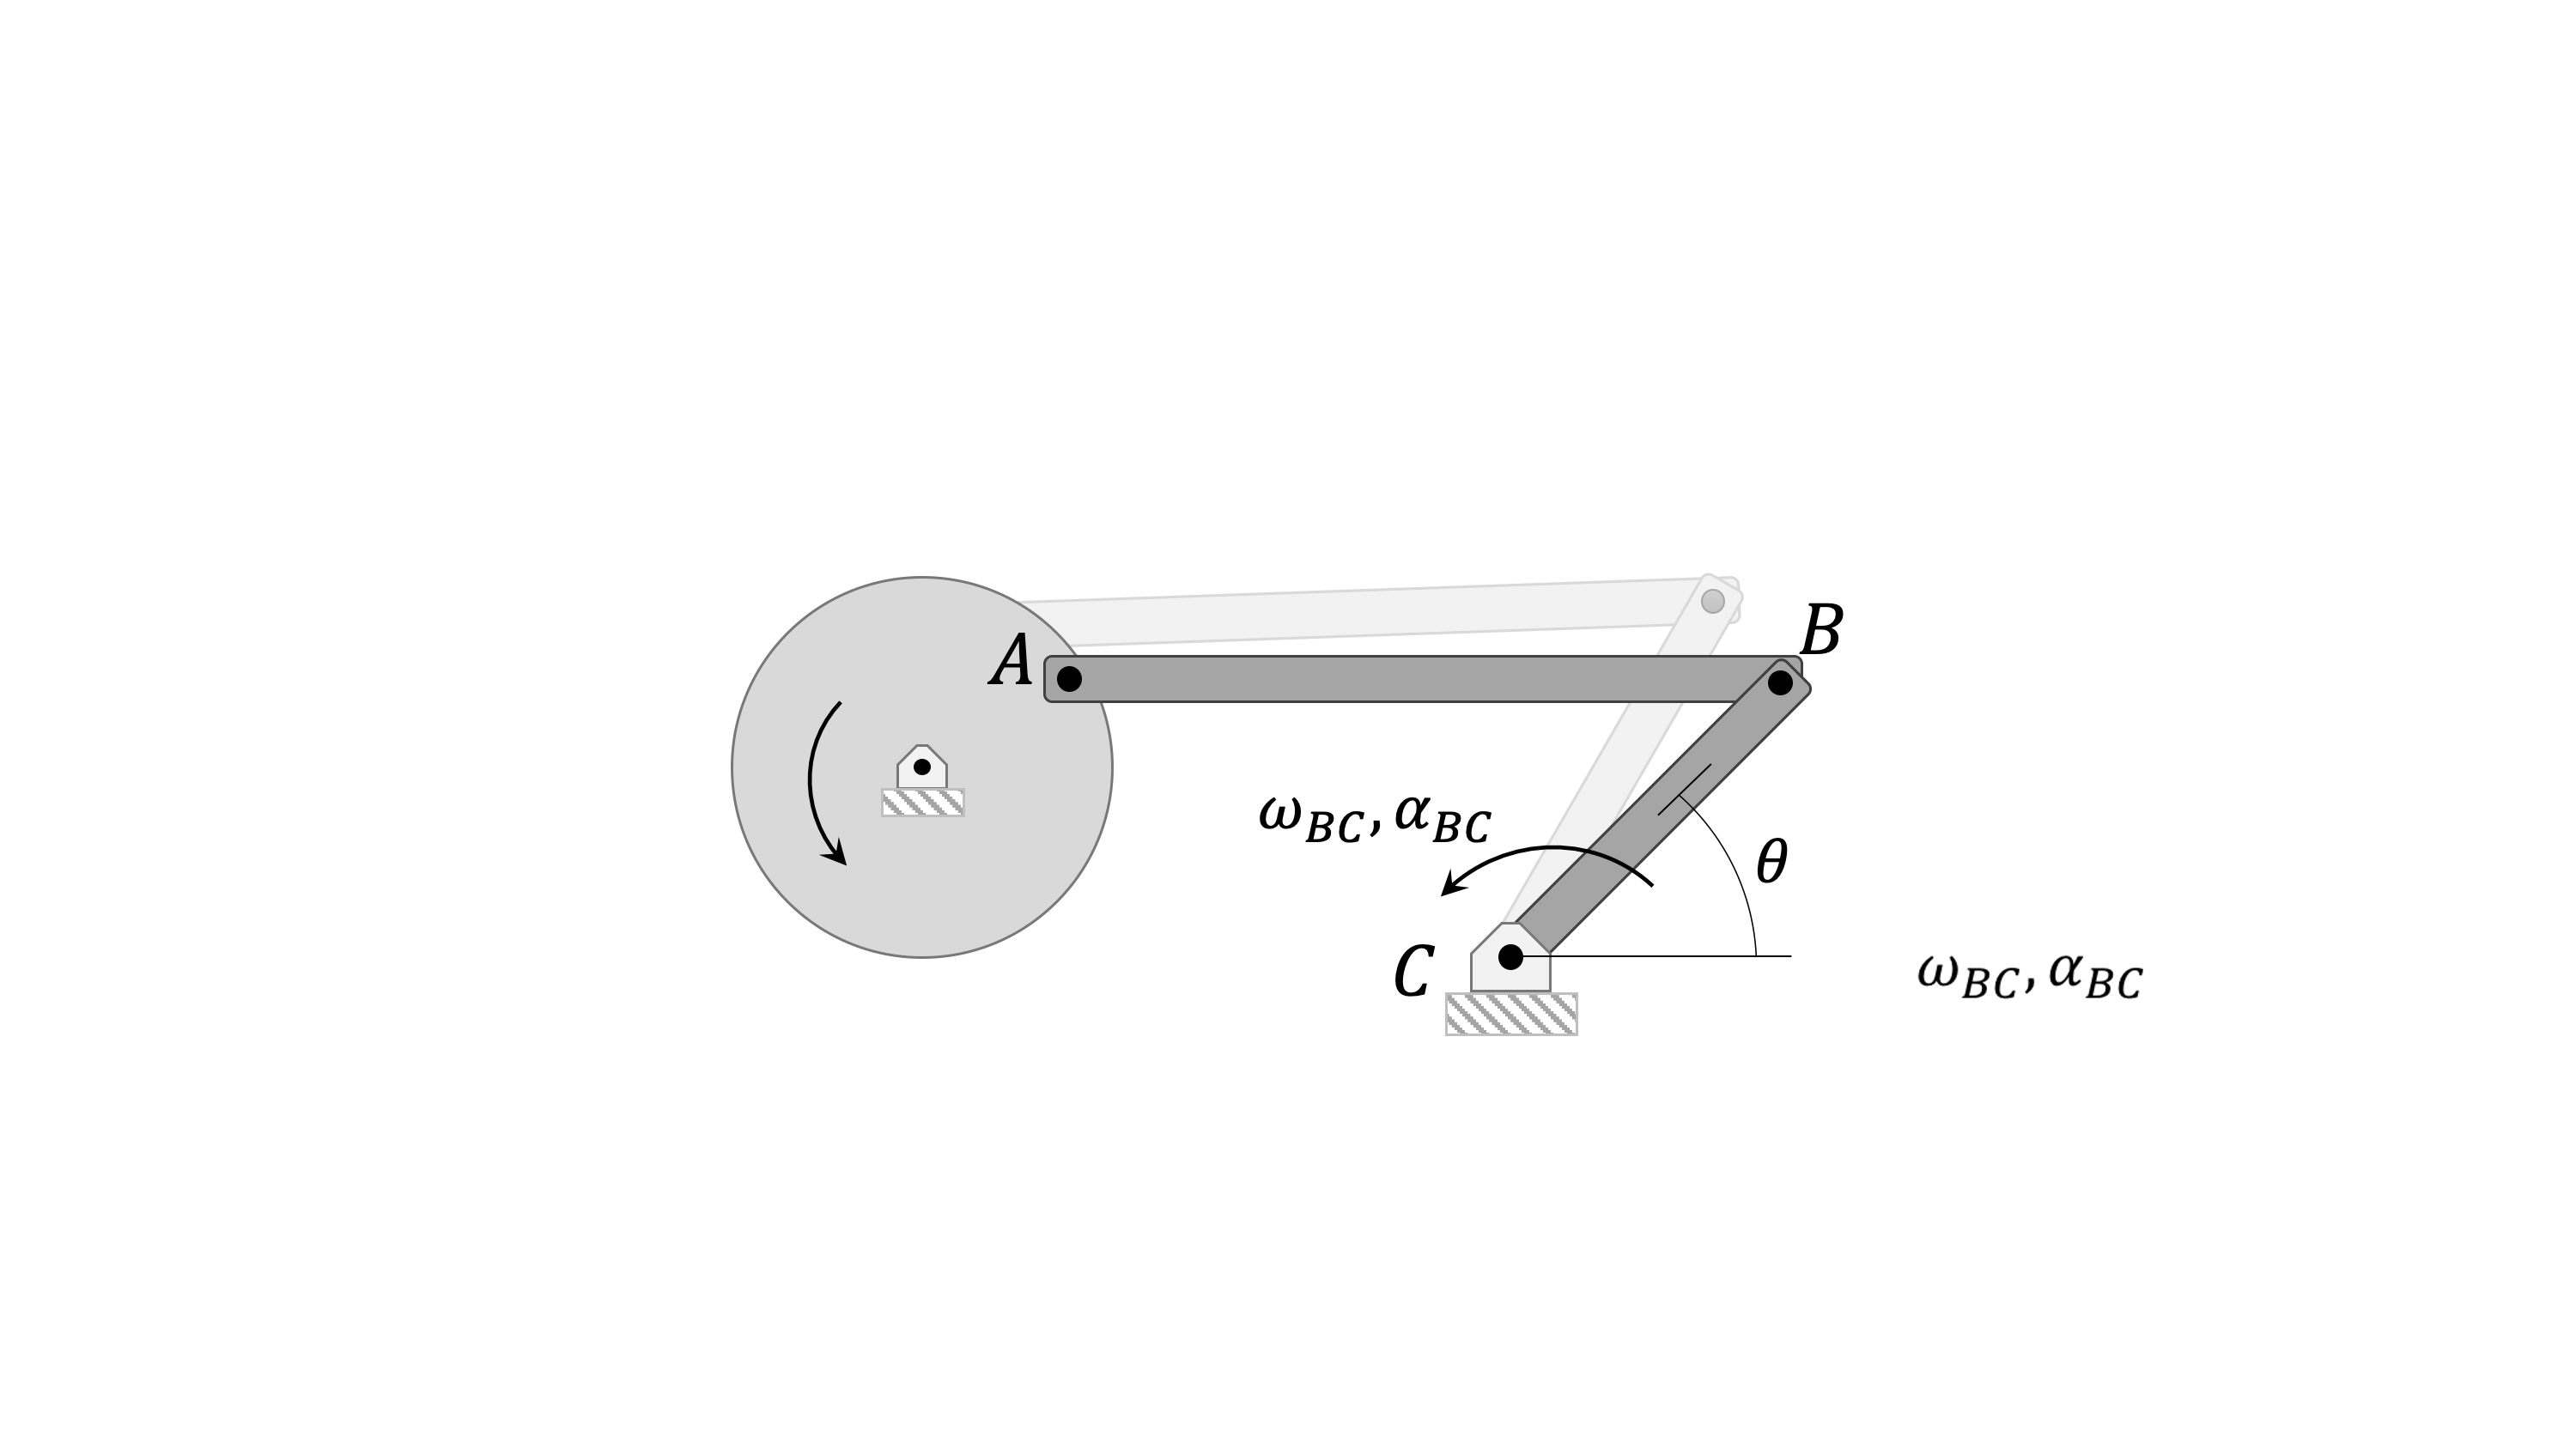
\includegraphics[trim={3cm 5cm 3cm 6cm},clip,width=0.8\textwidth, center]{Slide6}

By Chasles’ theorem, we know:
\[
\bm{v_B}= \bm{v_C} + \bm{\omega} \times \bm{r_{B/C}}\]
\raggedbottom
\newpage

\vspace*{5\baselineskip}

Compare with polar coordinate expression from particle kinematics: 
\[ \bm{v} = \dot{r}\bm{u_r} + r\dot{\theta}\bm{u_\theta}
\]

\vspace*{7\baselineskip}

For acceleration, recall:  
\[
\bm{a}=(\ddot{r}-r\dot{\theta^2})\bm{u_r}+(2\dot{r}\dot{\theta}+r\ddot{\theta})\bm{u_\theta}
\]

So, for \textbf{pure rigid body rotation} we are looking for an equation of the same form.

Differentiate: $ \bm{v_B}= \bm{\omega} \times \bm{r_{B/C}} $

\vspace*{14\baselineskip}

Components of acceleration for pure rotation:
\begin{center}
$\bm{\alpha} \times \bm{r_{B/C}} \Longleftrightarrow r\alpha\bm{u_\theta}$ - transverse component

$\bm{\omega} \times(\bm{\omega} \times \bm{r_{B/C}}) \Longleftrightarrow  -\omega^2r\bm{u_r}$ - centripedal component
\end{center}


(Note: for $\bm{a} \perp \bm{b}$: $\bm{a} \times(\bm{a}\times \bm{b}) = -a^2 \bm{b}$)


Thus: 
\[ \bm{a_B} = \bm{\alpha} \times \bm{r_{B/C}} - \omega^2 \bm{r_{B/C}} \]

Solve for the acceleration of point $B$, $\bm{a_B}$:
\vspace*{25\baselineskip}

\newpage
\section{Fixed Rotation:  Angular Relations}
In this section, we will establish parallel relationships between
distance/speed/acceleration
 and 
angle/angular speed/angular acceleration
\textbf{in a single direction (scalar)}


\begin{minipage}[c]{0.6\textwidth}
\begin{tabular}{  c  c }
\textbf{Angular:} & \textbf{Rectilinear:}\\
 &  \\
$\displaystyle \omega = \frac{d\theta}{dt}$ & $\displaystyle v = \frac{ds}{dt}$\\
 &  \\
$\displaystyle \alpha = \frac{d\omega}{dt}$ & $\displaystyle a = \frac{dv}{dt}$\\
& \\
& \\
 \hspace{1 cm} For $ \alpha = \alpha_c$ (constant): \hspace{1 cm} &  For $a = a_c$ (constant):\\
 & \\
 & $s = s_0 + v_0 t+\frac{1}{2} a_c t^2$\\
  &  \\
 & $v = v_0 + a_c t$\\
 & \\
 & $v^2 = v_0^2 + 2 a_c(s-s_0)$\\
\end{tabular}
\label{tab:singlebest}
\end{minipage}%%%
\begin{minipage}[c]{0.45\textwidth}
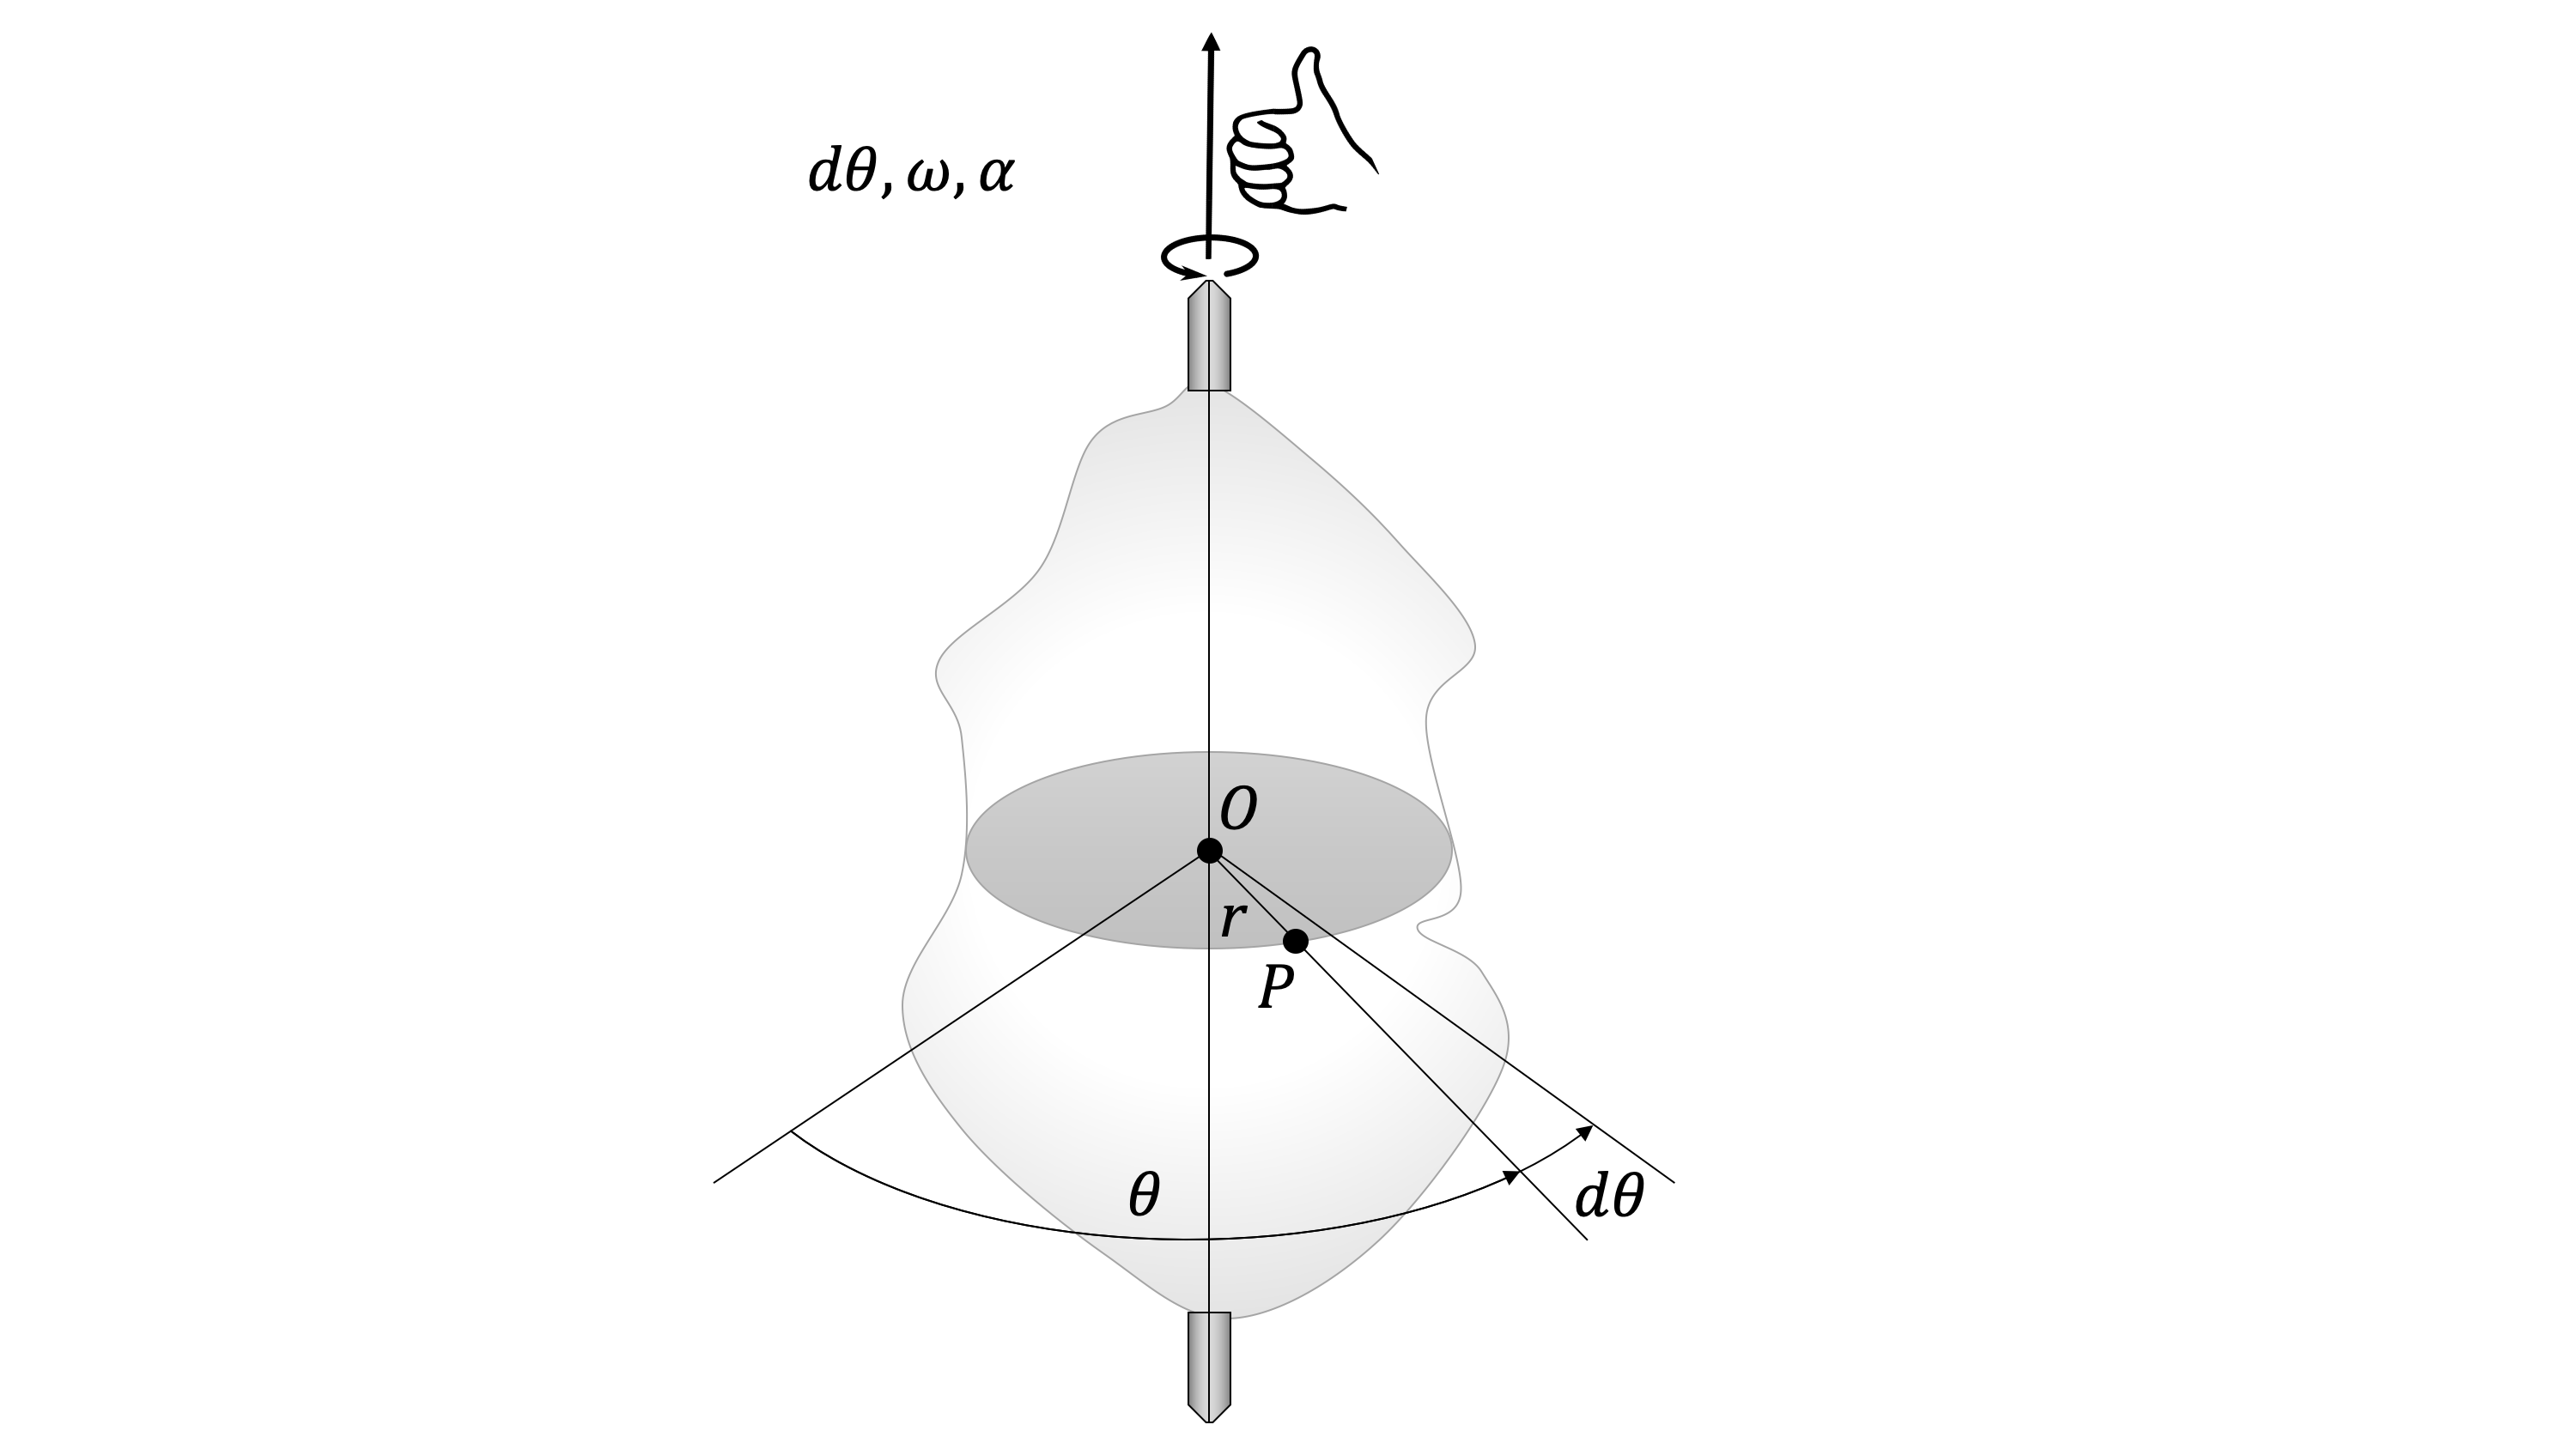
\includegraphics[trim={10cm 0cm 12cm 0cm},clip,width=0.7\textwidth, center]{Slide8} 
\end{minipage}

Important Note:  Angular velocity and angular acceleration FOR A RIGID BODY is the SAME for EVERY POINT on the body

\subsection{Example}
\begin{minipage}[l]{0.4\textwidth}
Gear $A$ and $B$ mesh as shown.  A starts from rest, with constant angular acceleration $\alpha_A=2 \, rad/s^2$. How long does it take $B$ to reach $\omega_B=50 \, rad/s$?
\end{minipage}
\begin{minipage}[c]{0.6\textwidth}
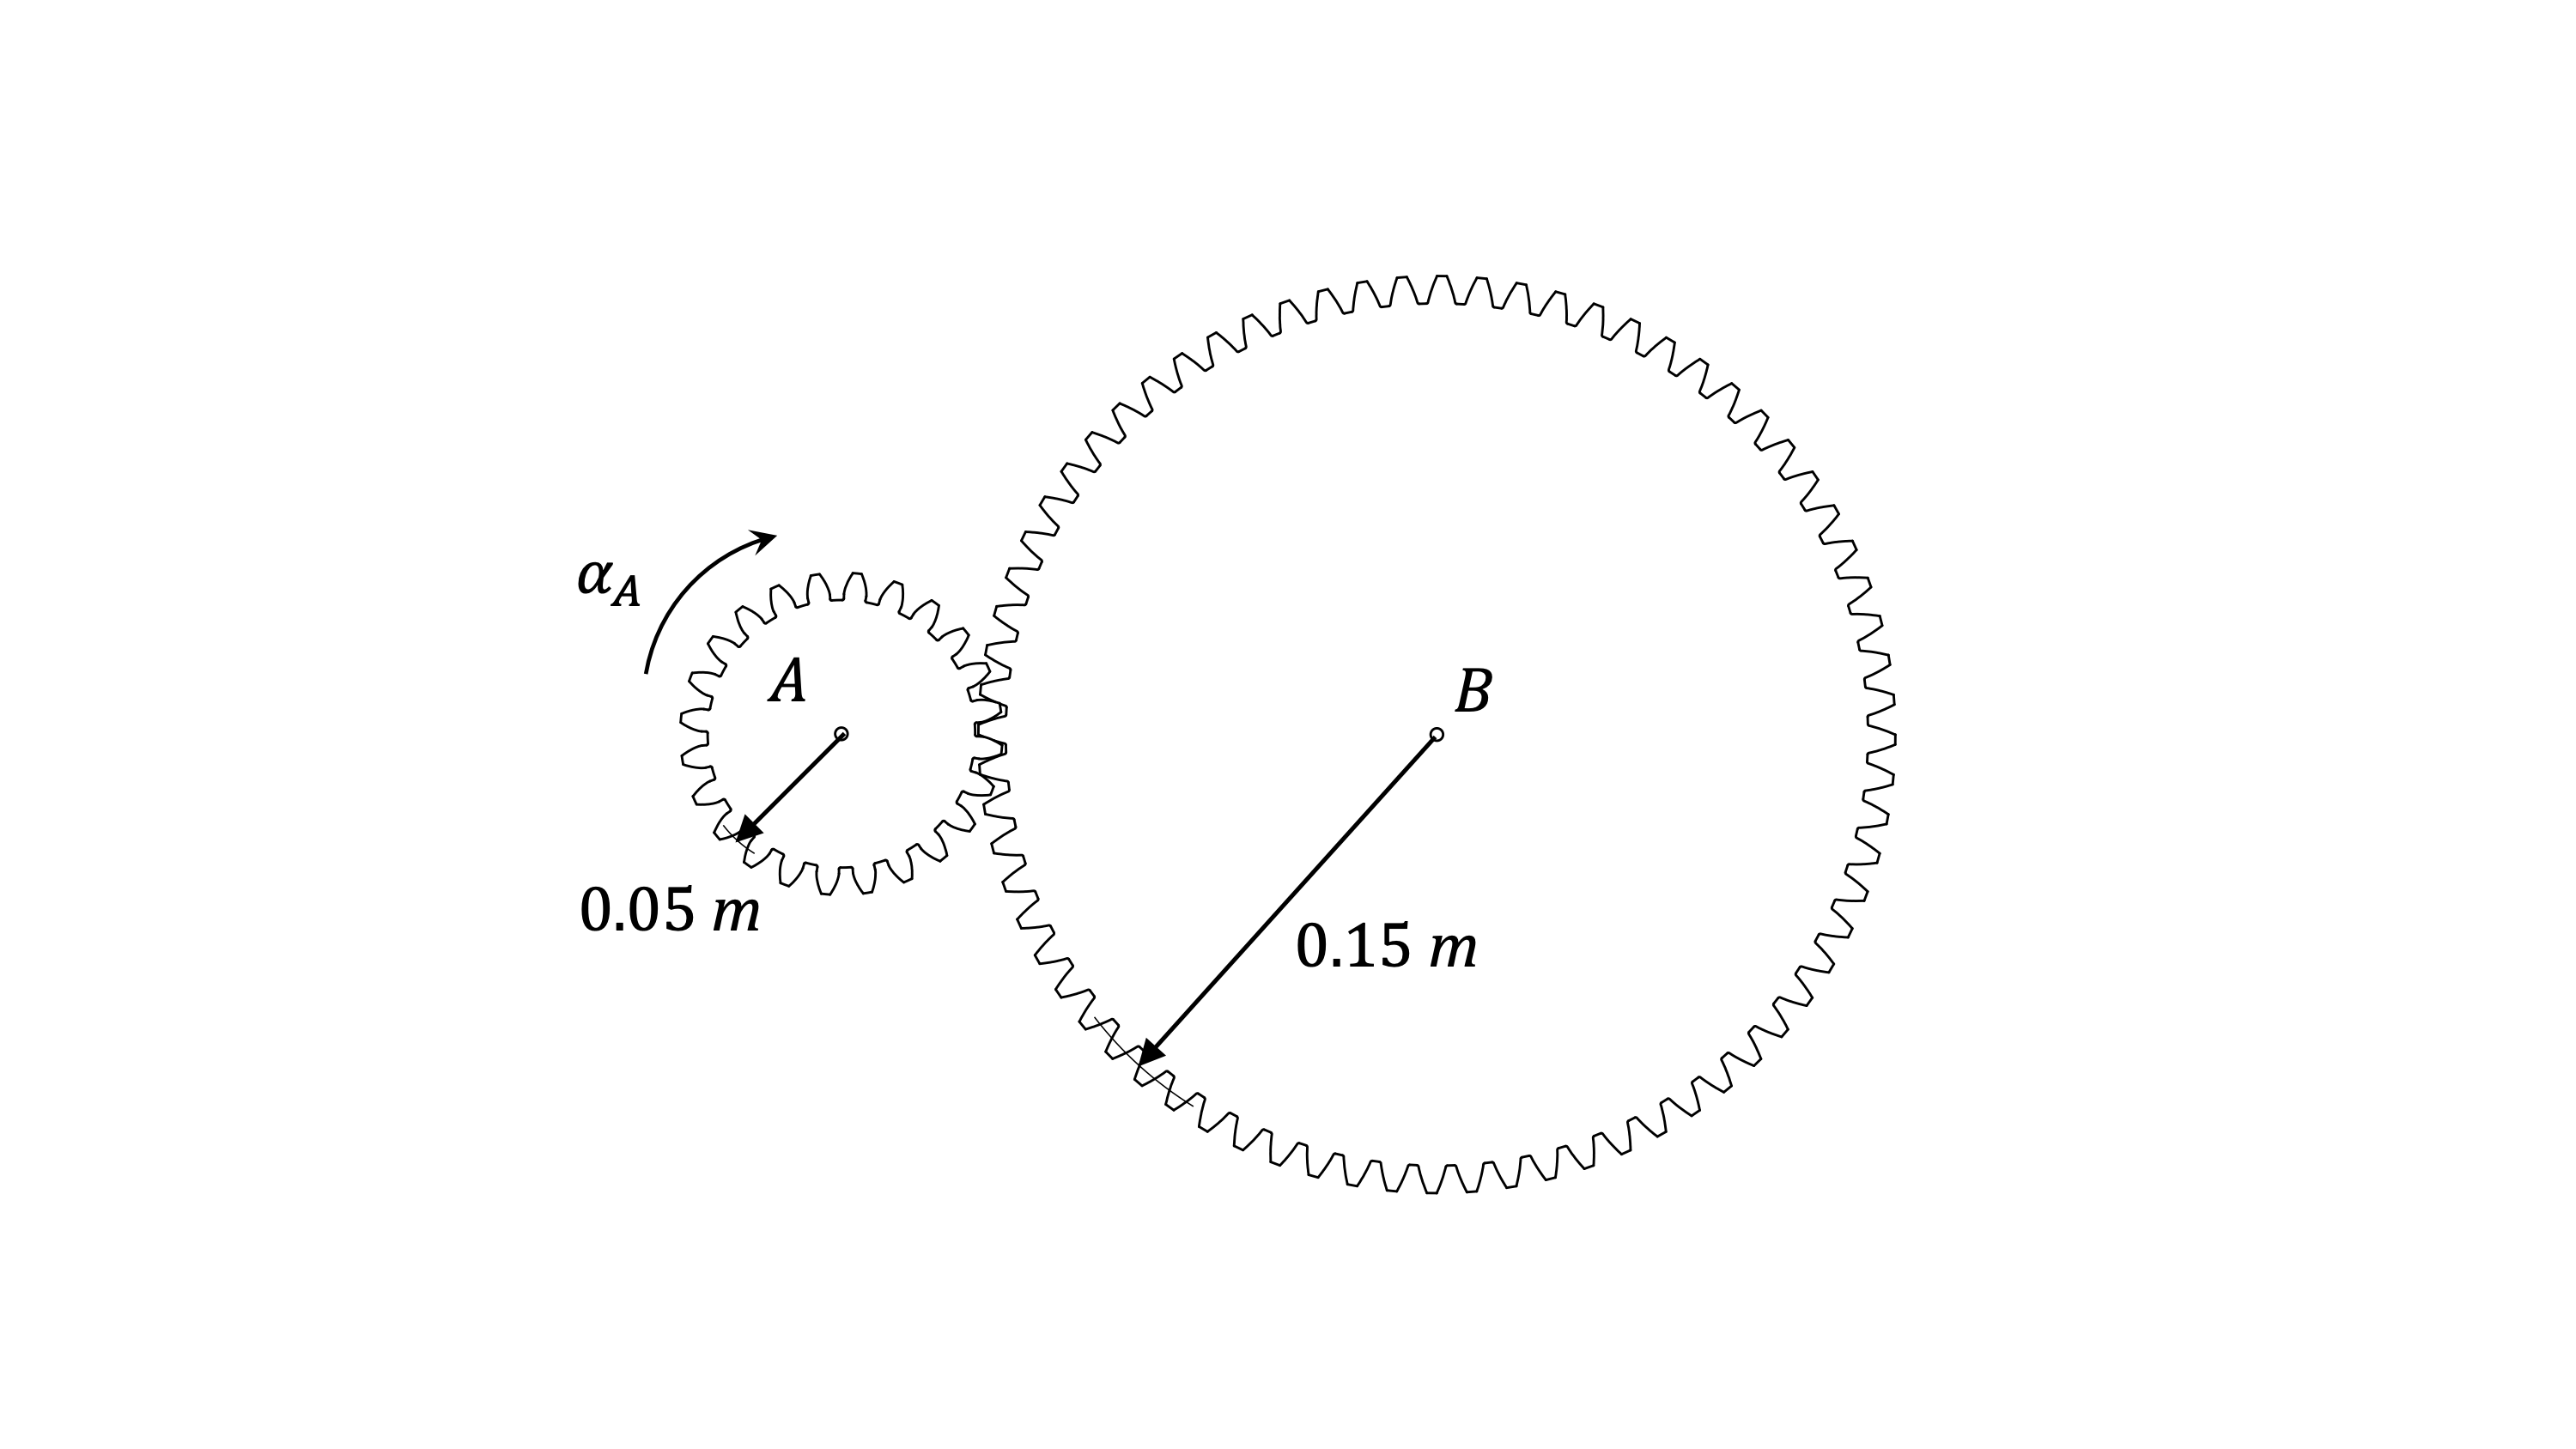
\includegraphics[trim={7cm 3cm 8cm 3cm},clip,width=0.9\textwidth, center]{Slide10}
\end{minipage}

\newpage

(Example continued)

\newpage

\chapter{L2: Relative Plane Motion Analysis - Velocity}
Readings

\section{Objective}
To describe the motion of a point on a rigid body using a translating reference frame attached to the body.

\section{Fixed and Translating Reference Frames}
In this section we consider a frame $x'y'$ attached to a body at a point $A$ as if by a pin – i.e.: translating but NOT rotating with the body. $xy$ is a fixed frame (attached to ground). 

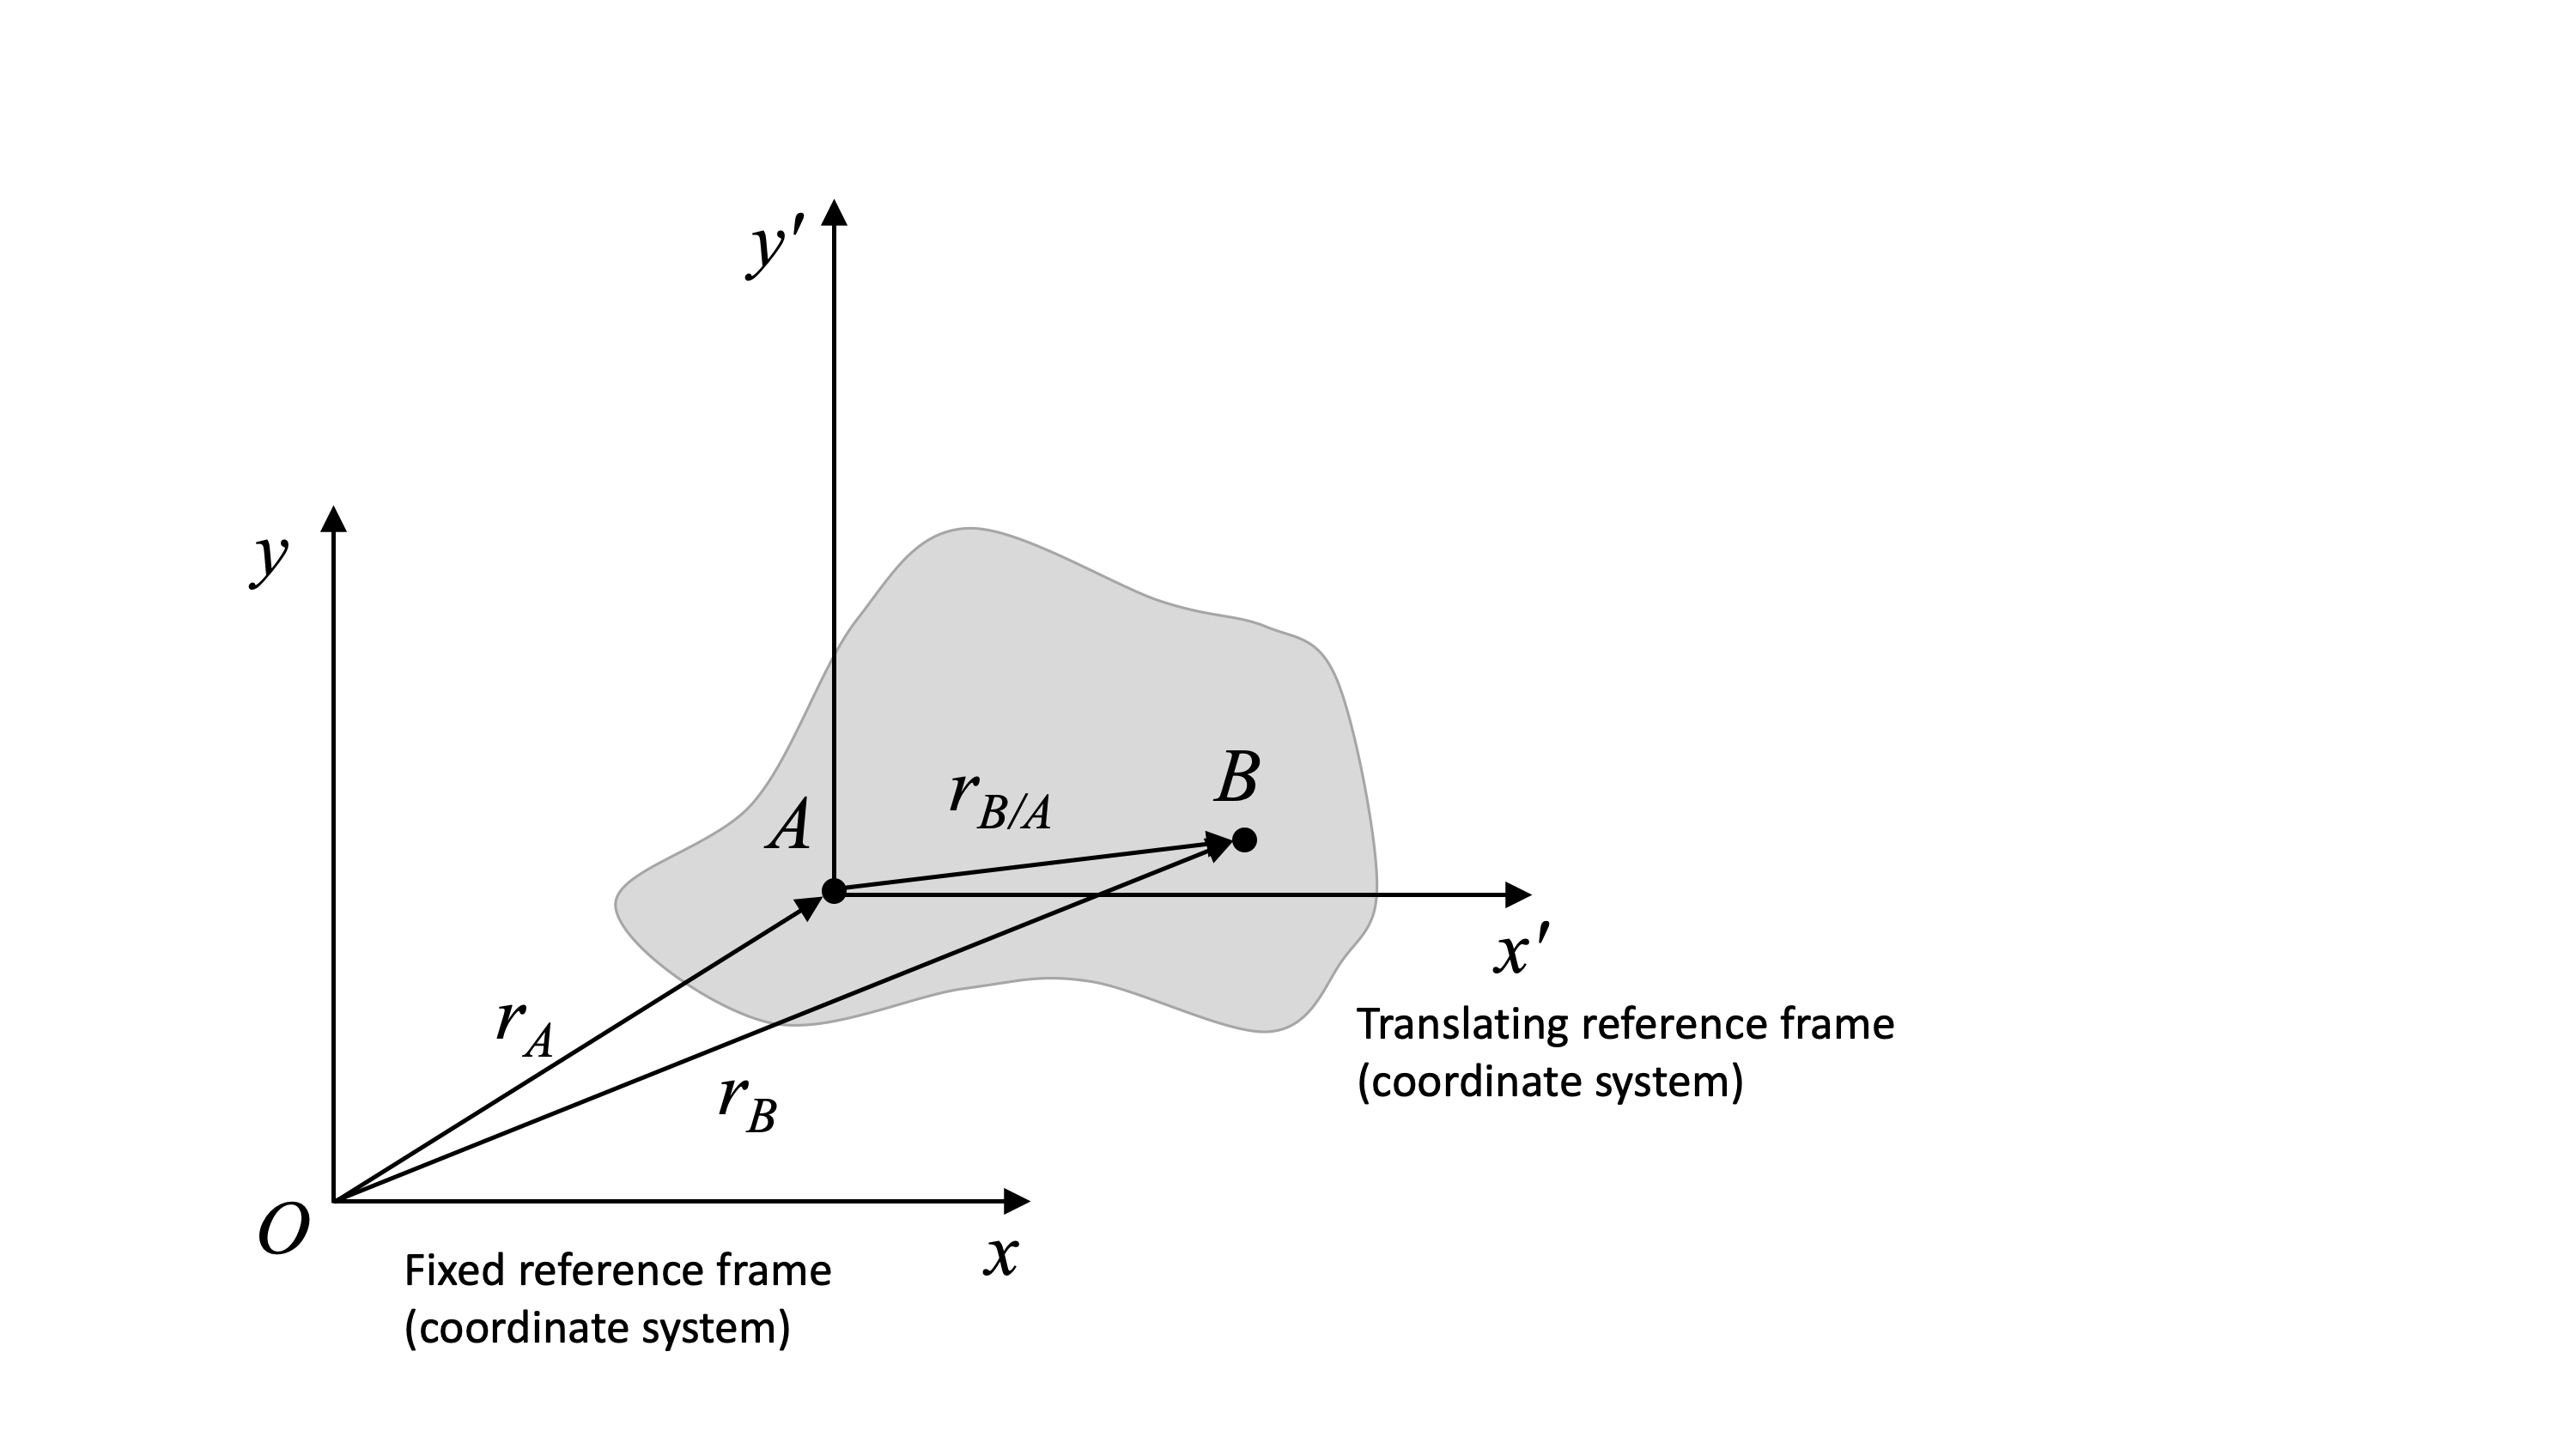
\includegraphics[trim={3cm 0cm 7.5cm 1.5cm},clip,width=0.55\textwidth, center]{Slide5}


\begin{center}
\begin{tabu} to 1\textwidth {  X[c]  X[c] X[c] X[c]  X[c]  }
$\bm{r_A}$ & $+$ & $\bm{r_{B/A}}$ & $=$ & $\bm{r_B}$\\
 & & & & \\
Describes the location of the translating reference frame  $x'y'$ with respect to the fixed $xy$ frame & $+$ & Describes the location of point B with respect to translating reference frame $x'y'$ & $=$ & Describes the location of point B with respect to the fixed frame $xy$\\
\end{tabu}
\end{center}

\newpage

IMPORTANT NOTE: "with respect to" means "measured from".  BUT we must make sure we are using the \textbf{same axis directions} to do the measurements. 

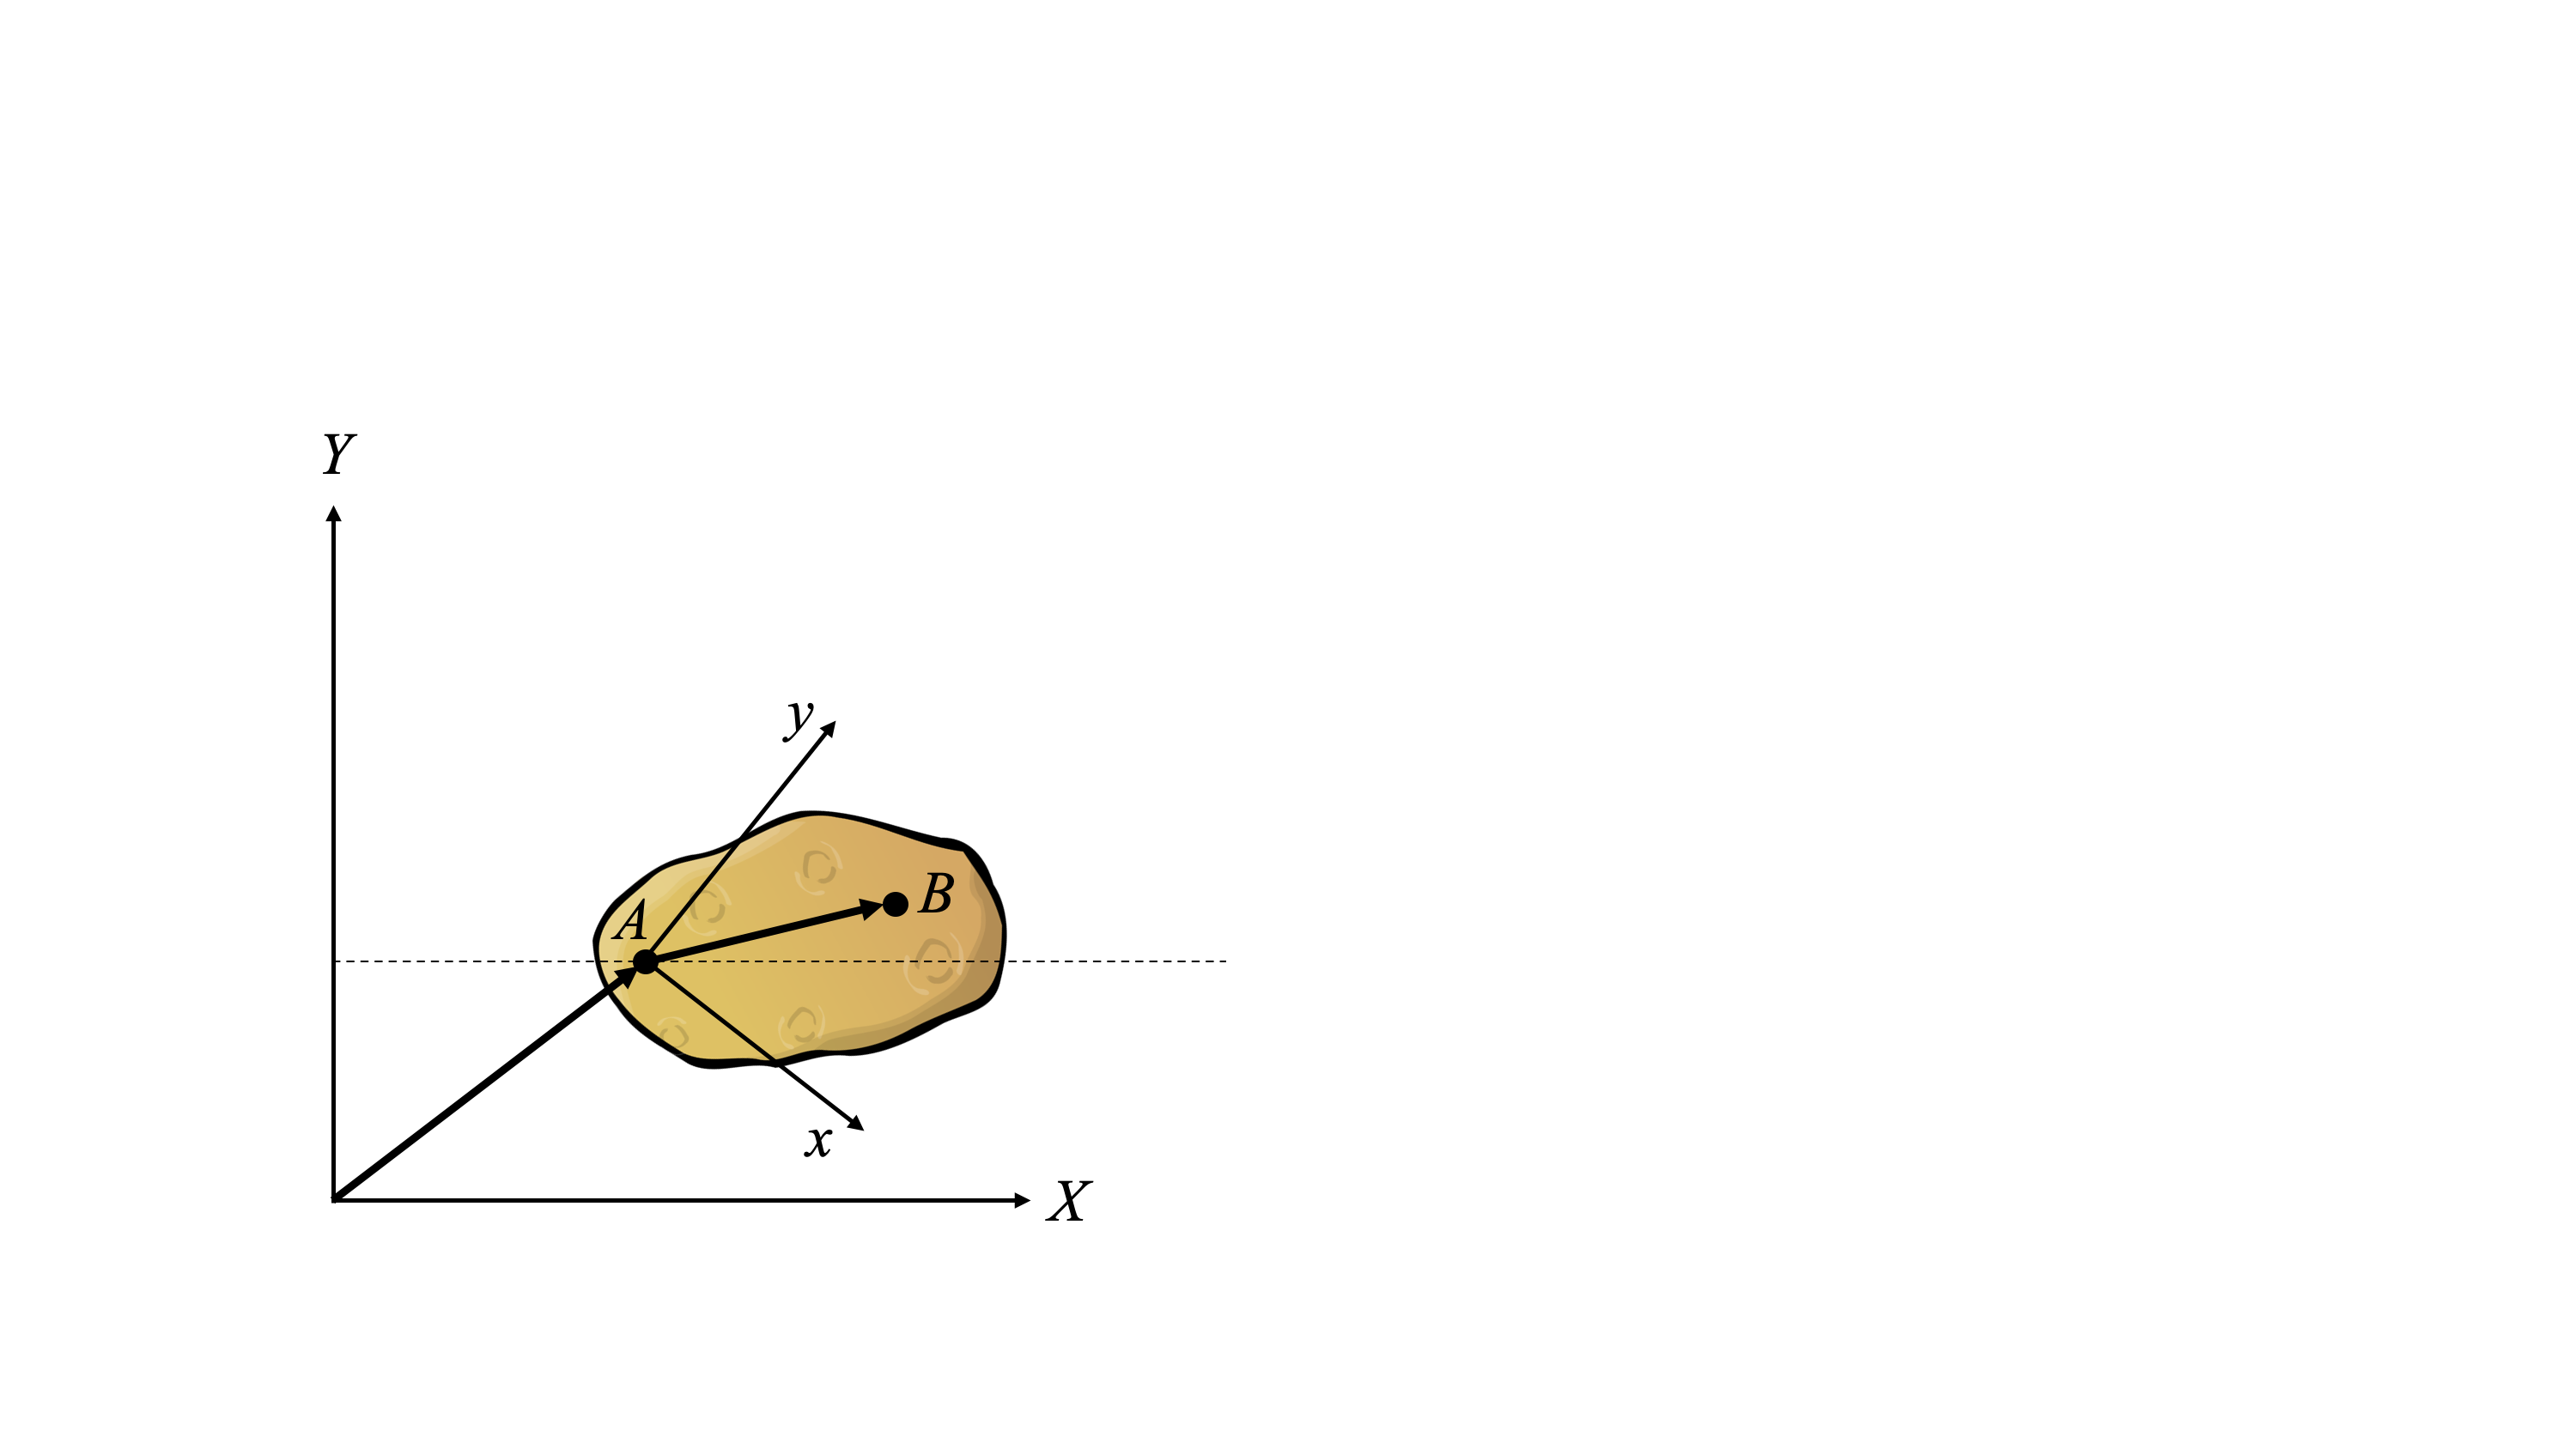
\includegraphics[trim={3cm 0cm 14cm 5cm},clip,width=0.55\textwidth, center]{Slide12}

As before, we differentiate position to get velocity.  

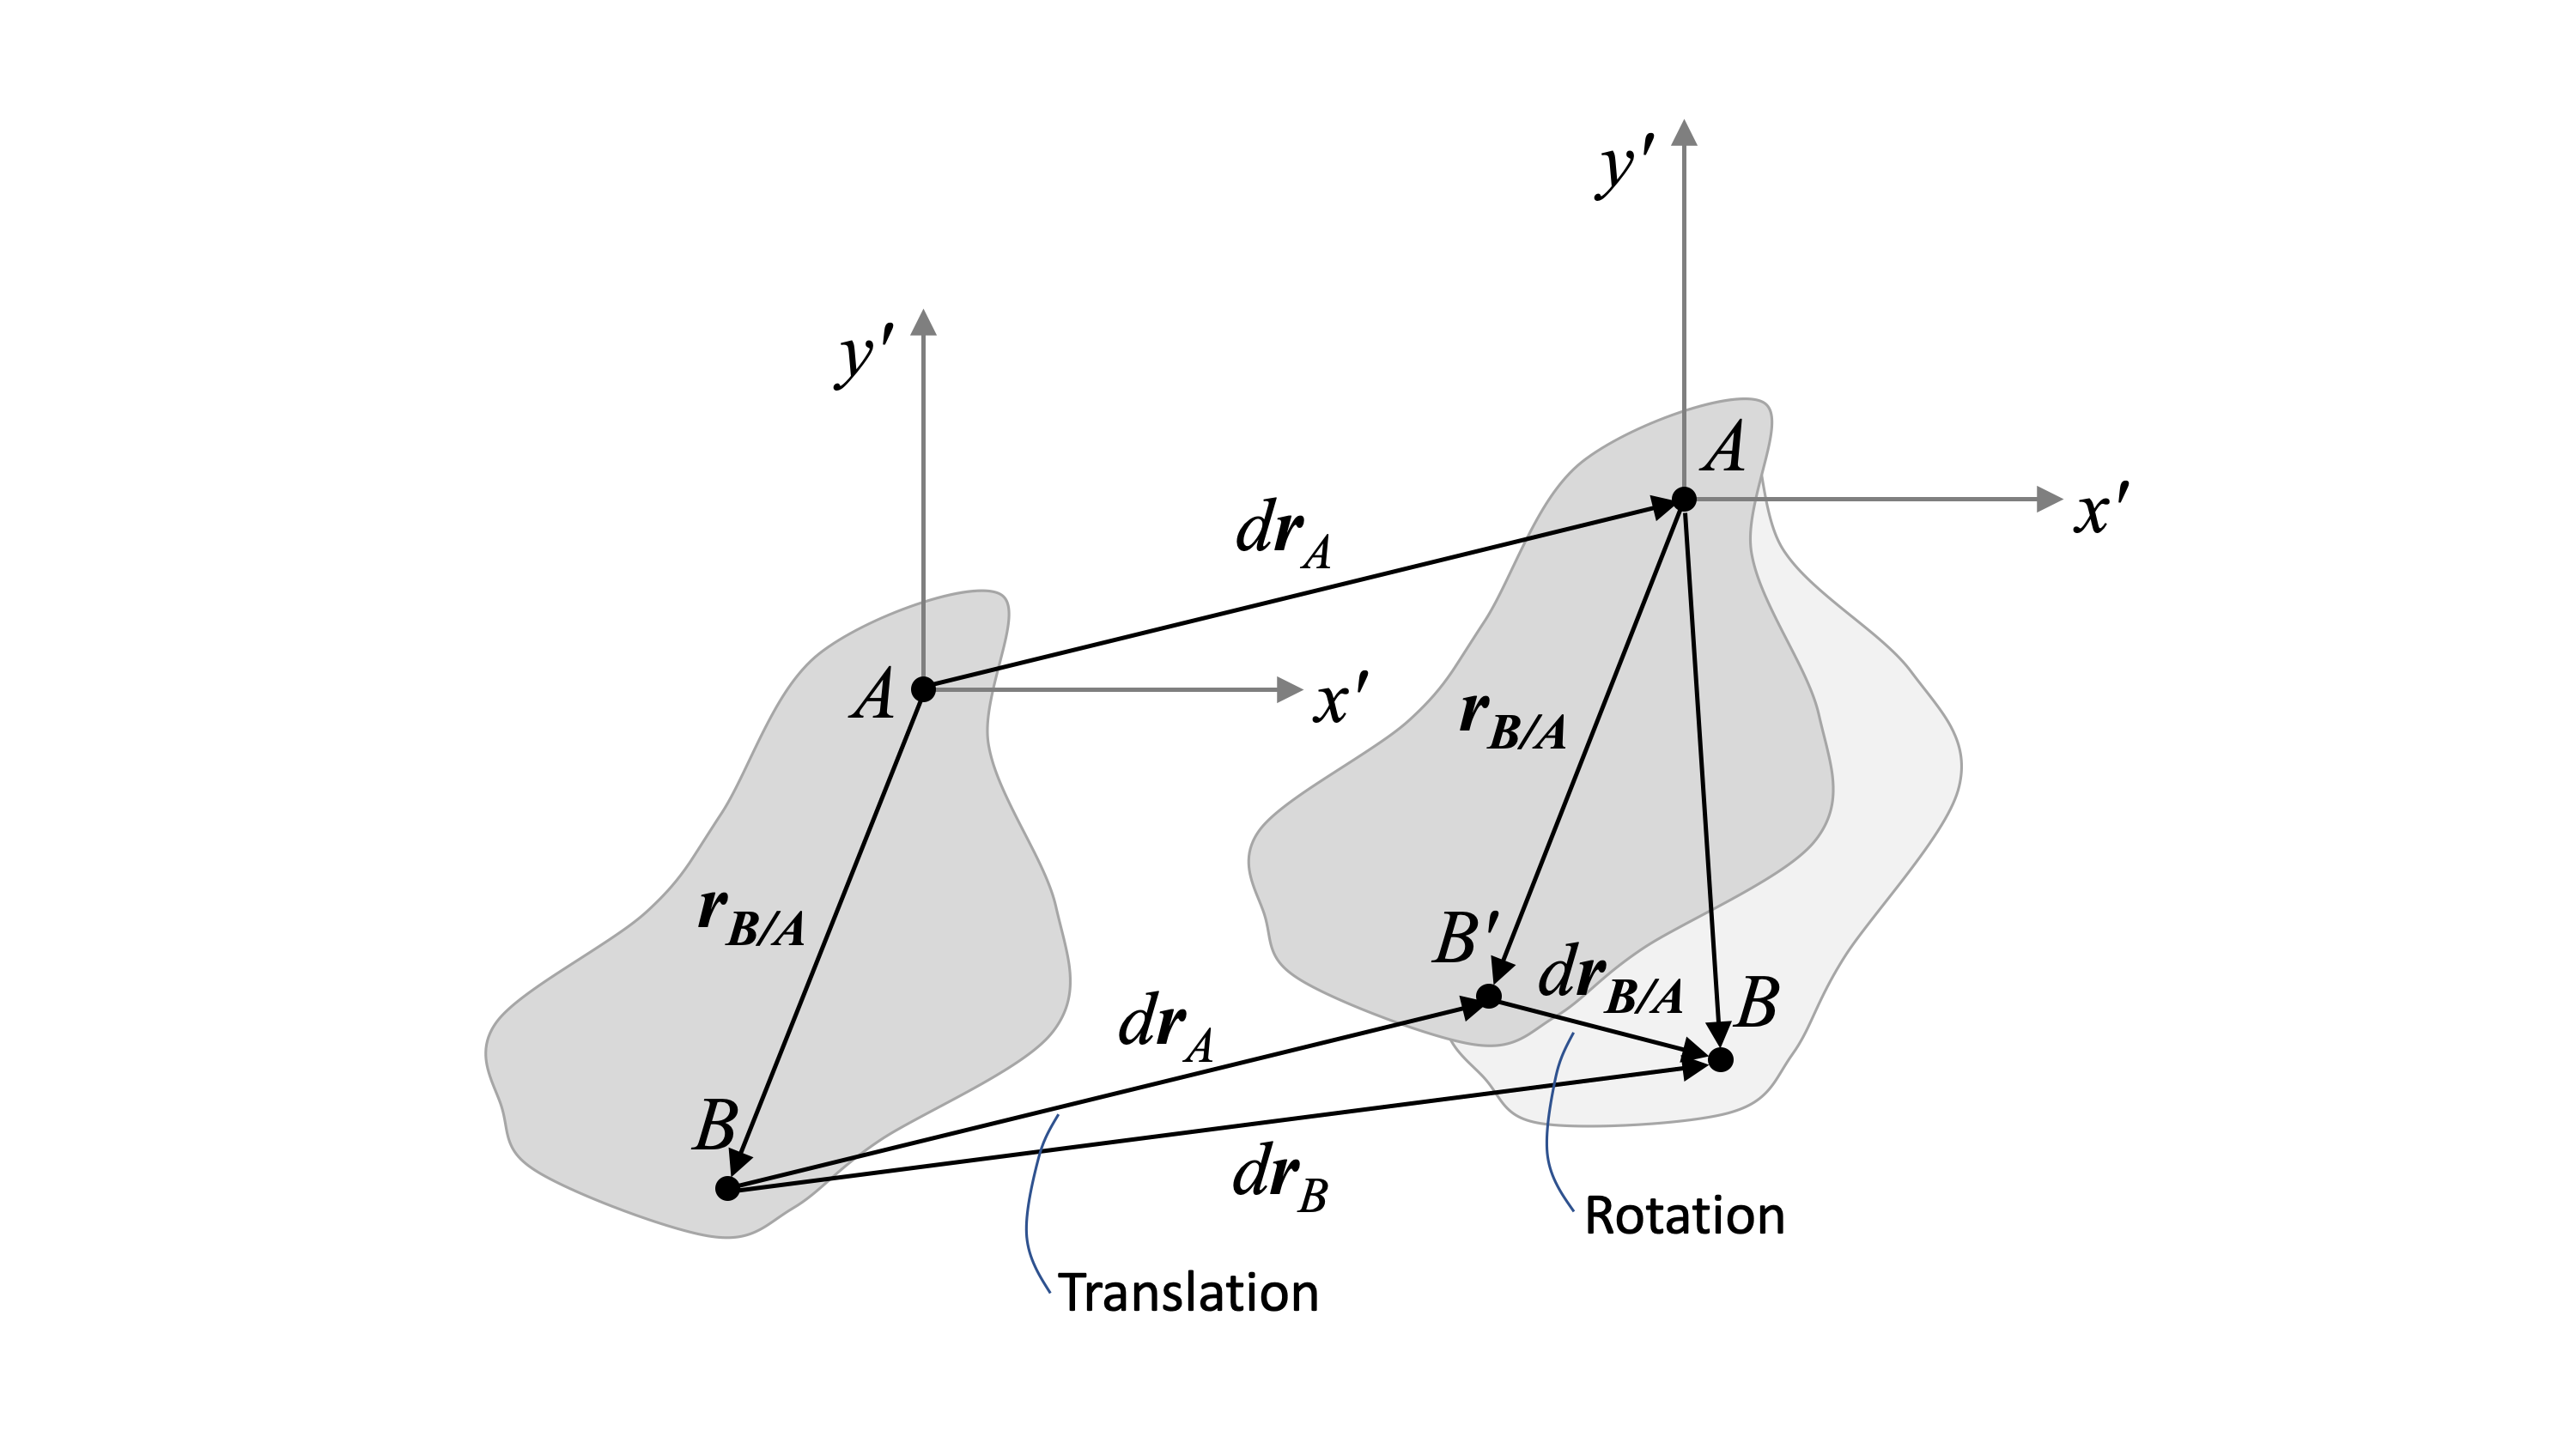
\includegraphics[trim={0cm 0cm 0cm 1.5cm},clip,width=0.9\textwidth, center]{Slide13}

Since the body is rigid (i.e. does not change size), the magnitude of $\bm{r_{B/A}}$ must be constant. Therefore, $\displaystyle \bm{v_{B/A}} = \frac{d\bm{r_{B/A}}}{dt}$ is due only to the \textbf{rotation} of point $B$ about point $A$.  That is, the motion follows Chasles' theorem:
\[ \bm{v_B}=\bm{v_A} + \bm{\omega} \times \bm{r_{B/A}} \]
\raggedbottom

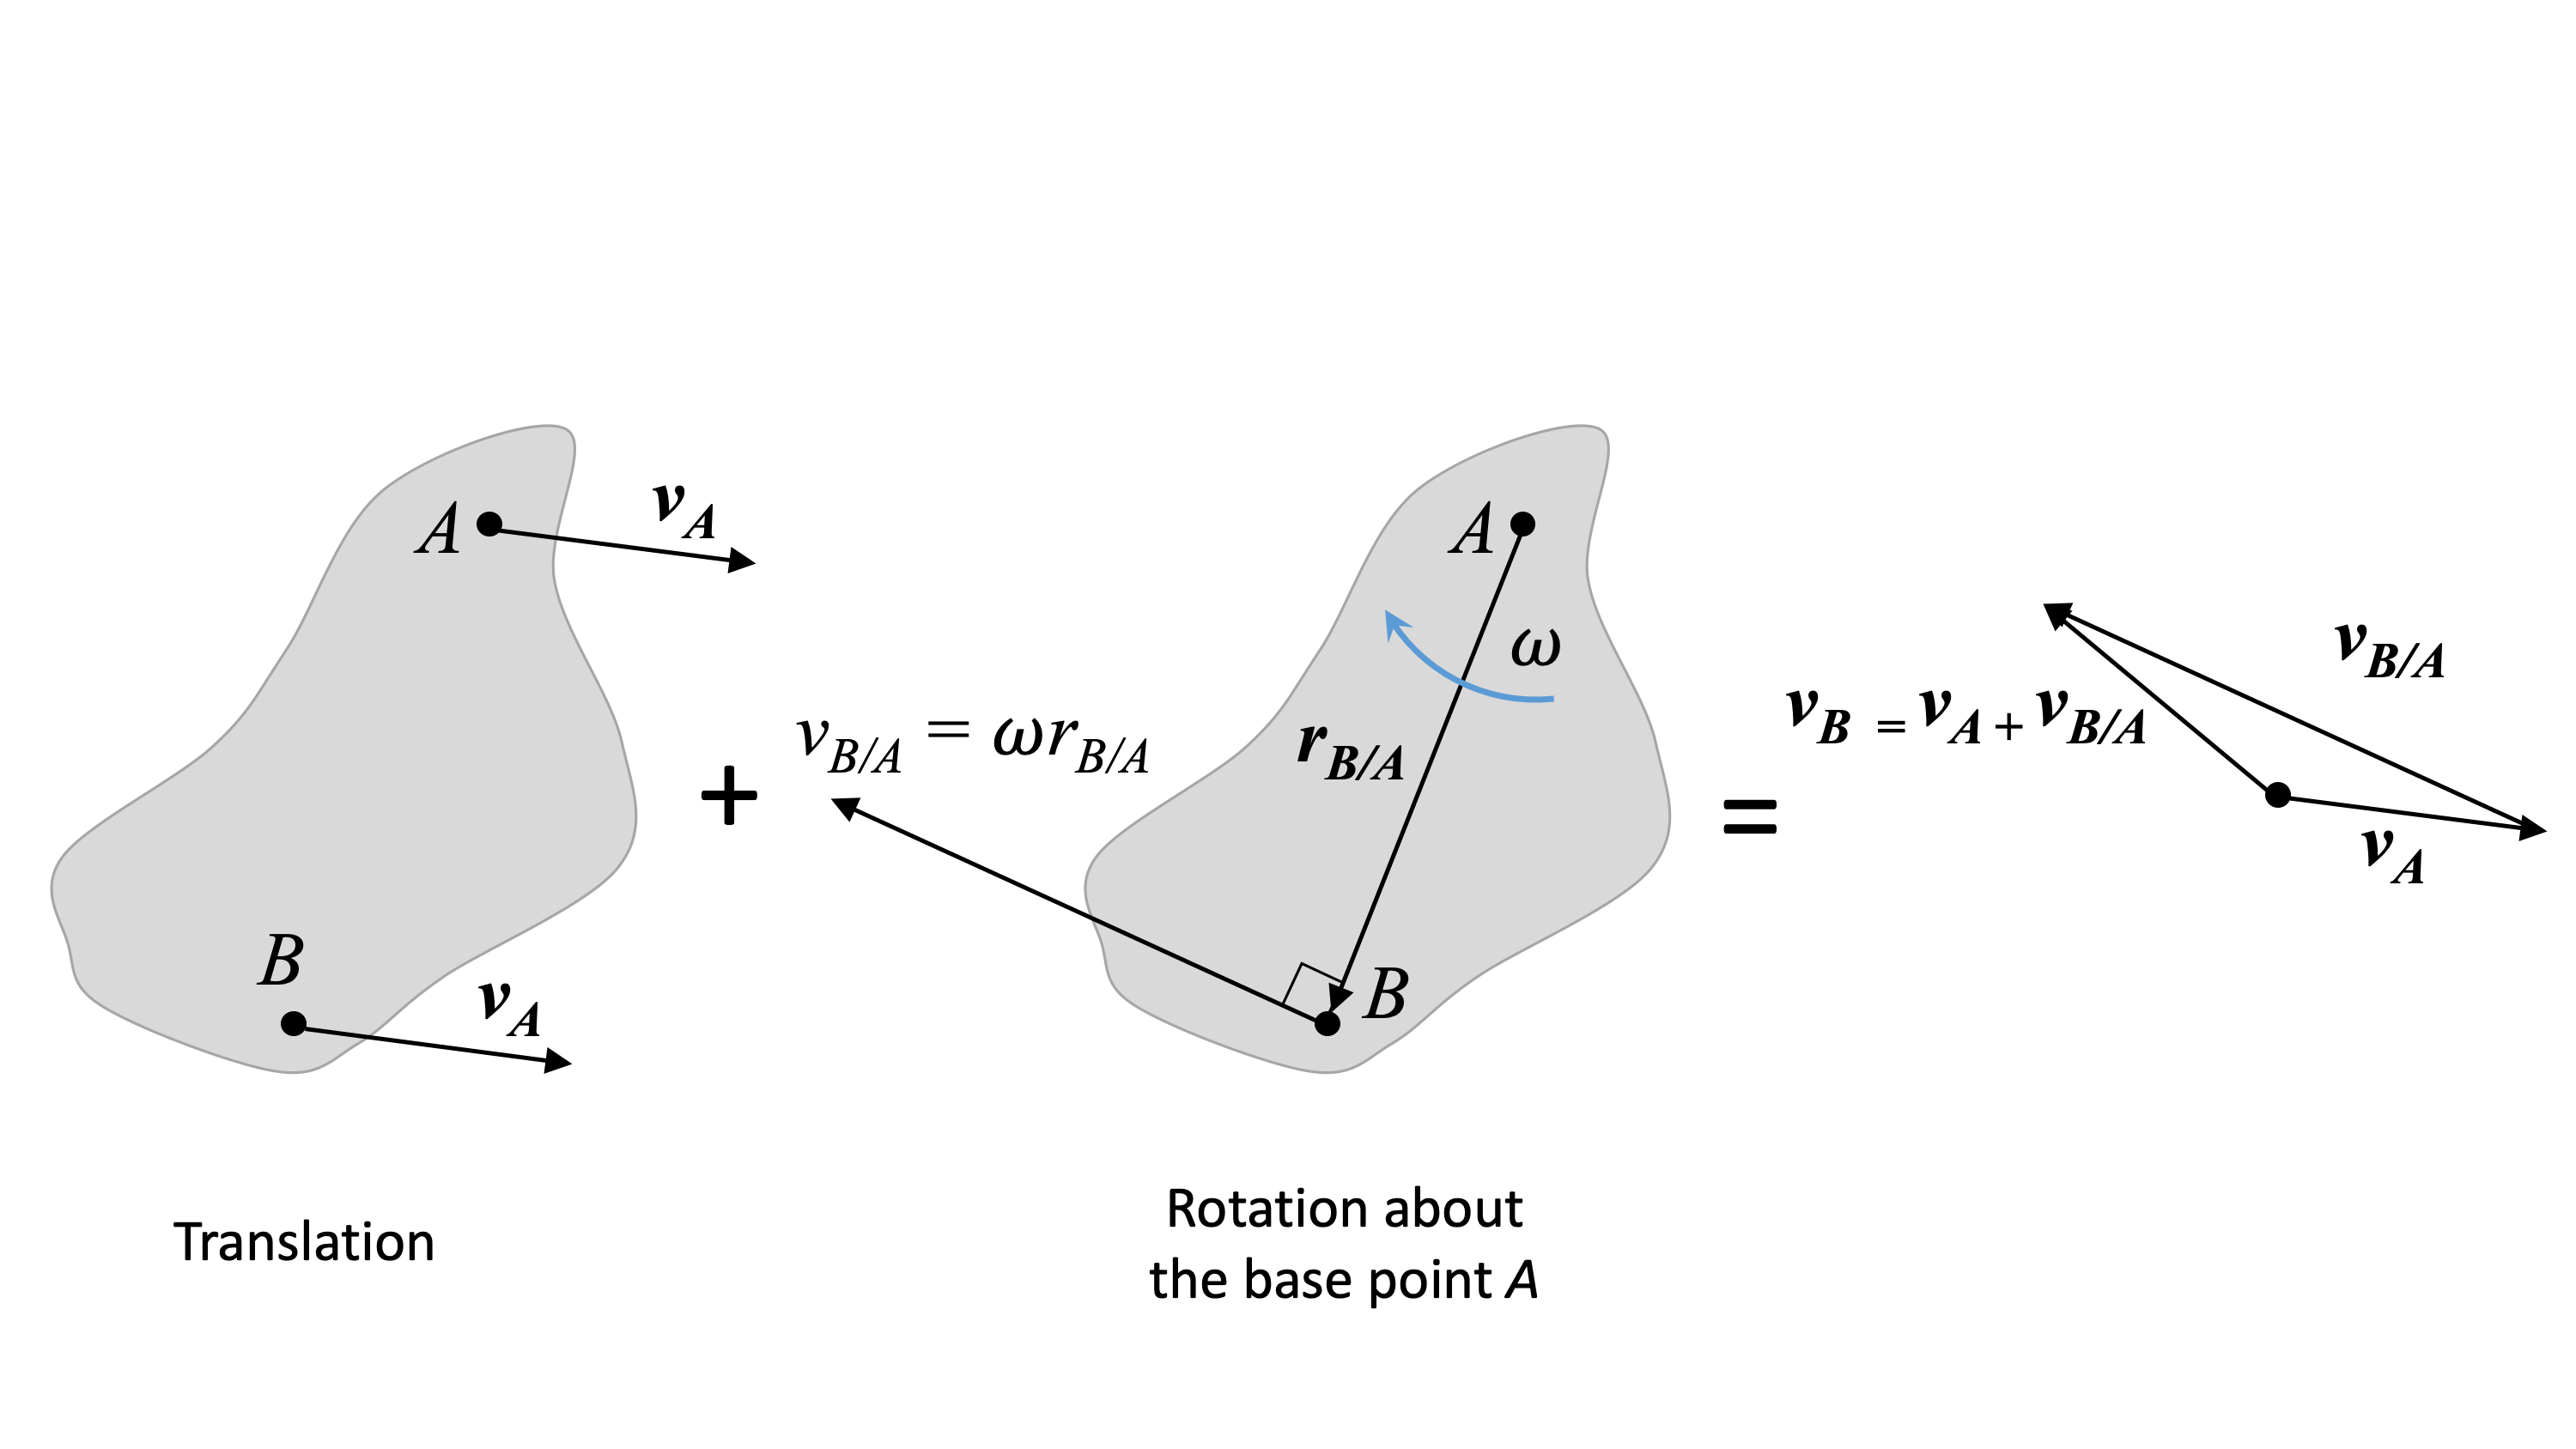
\includegraphics[trim={0cm 1cm 0cm 4cm},clip,width=0.9\textwidth, center]{Slide14}

\subsection{Example}
Find $\bm{\omega_{BC}}$ and $\bm{v_C}$ at the instant shown.  $\theta = 60^{\circ}$.

\begin{minipage}[l]{0.6\textwidth}
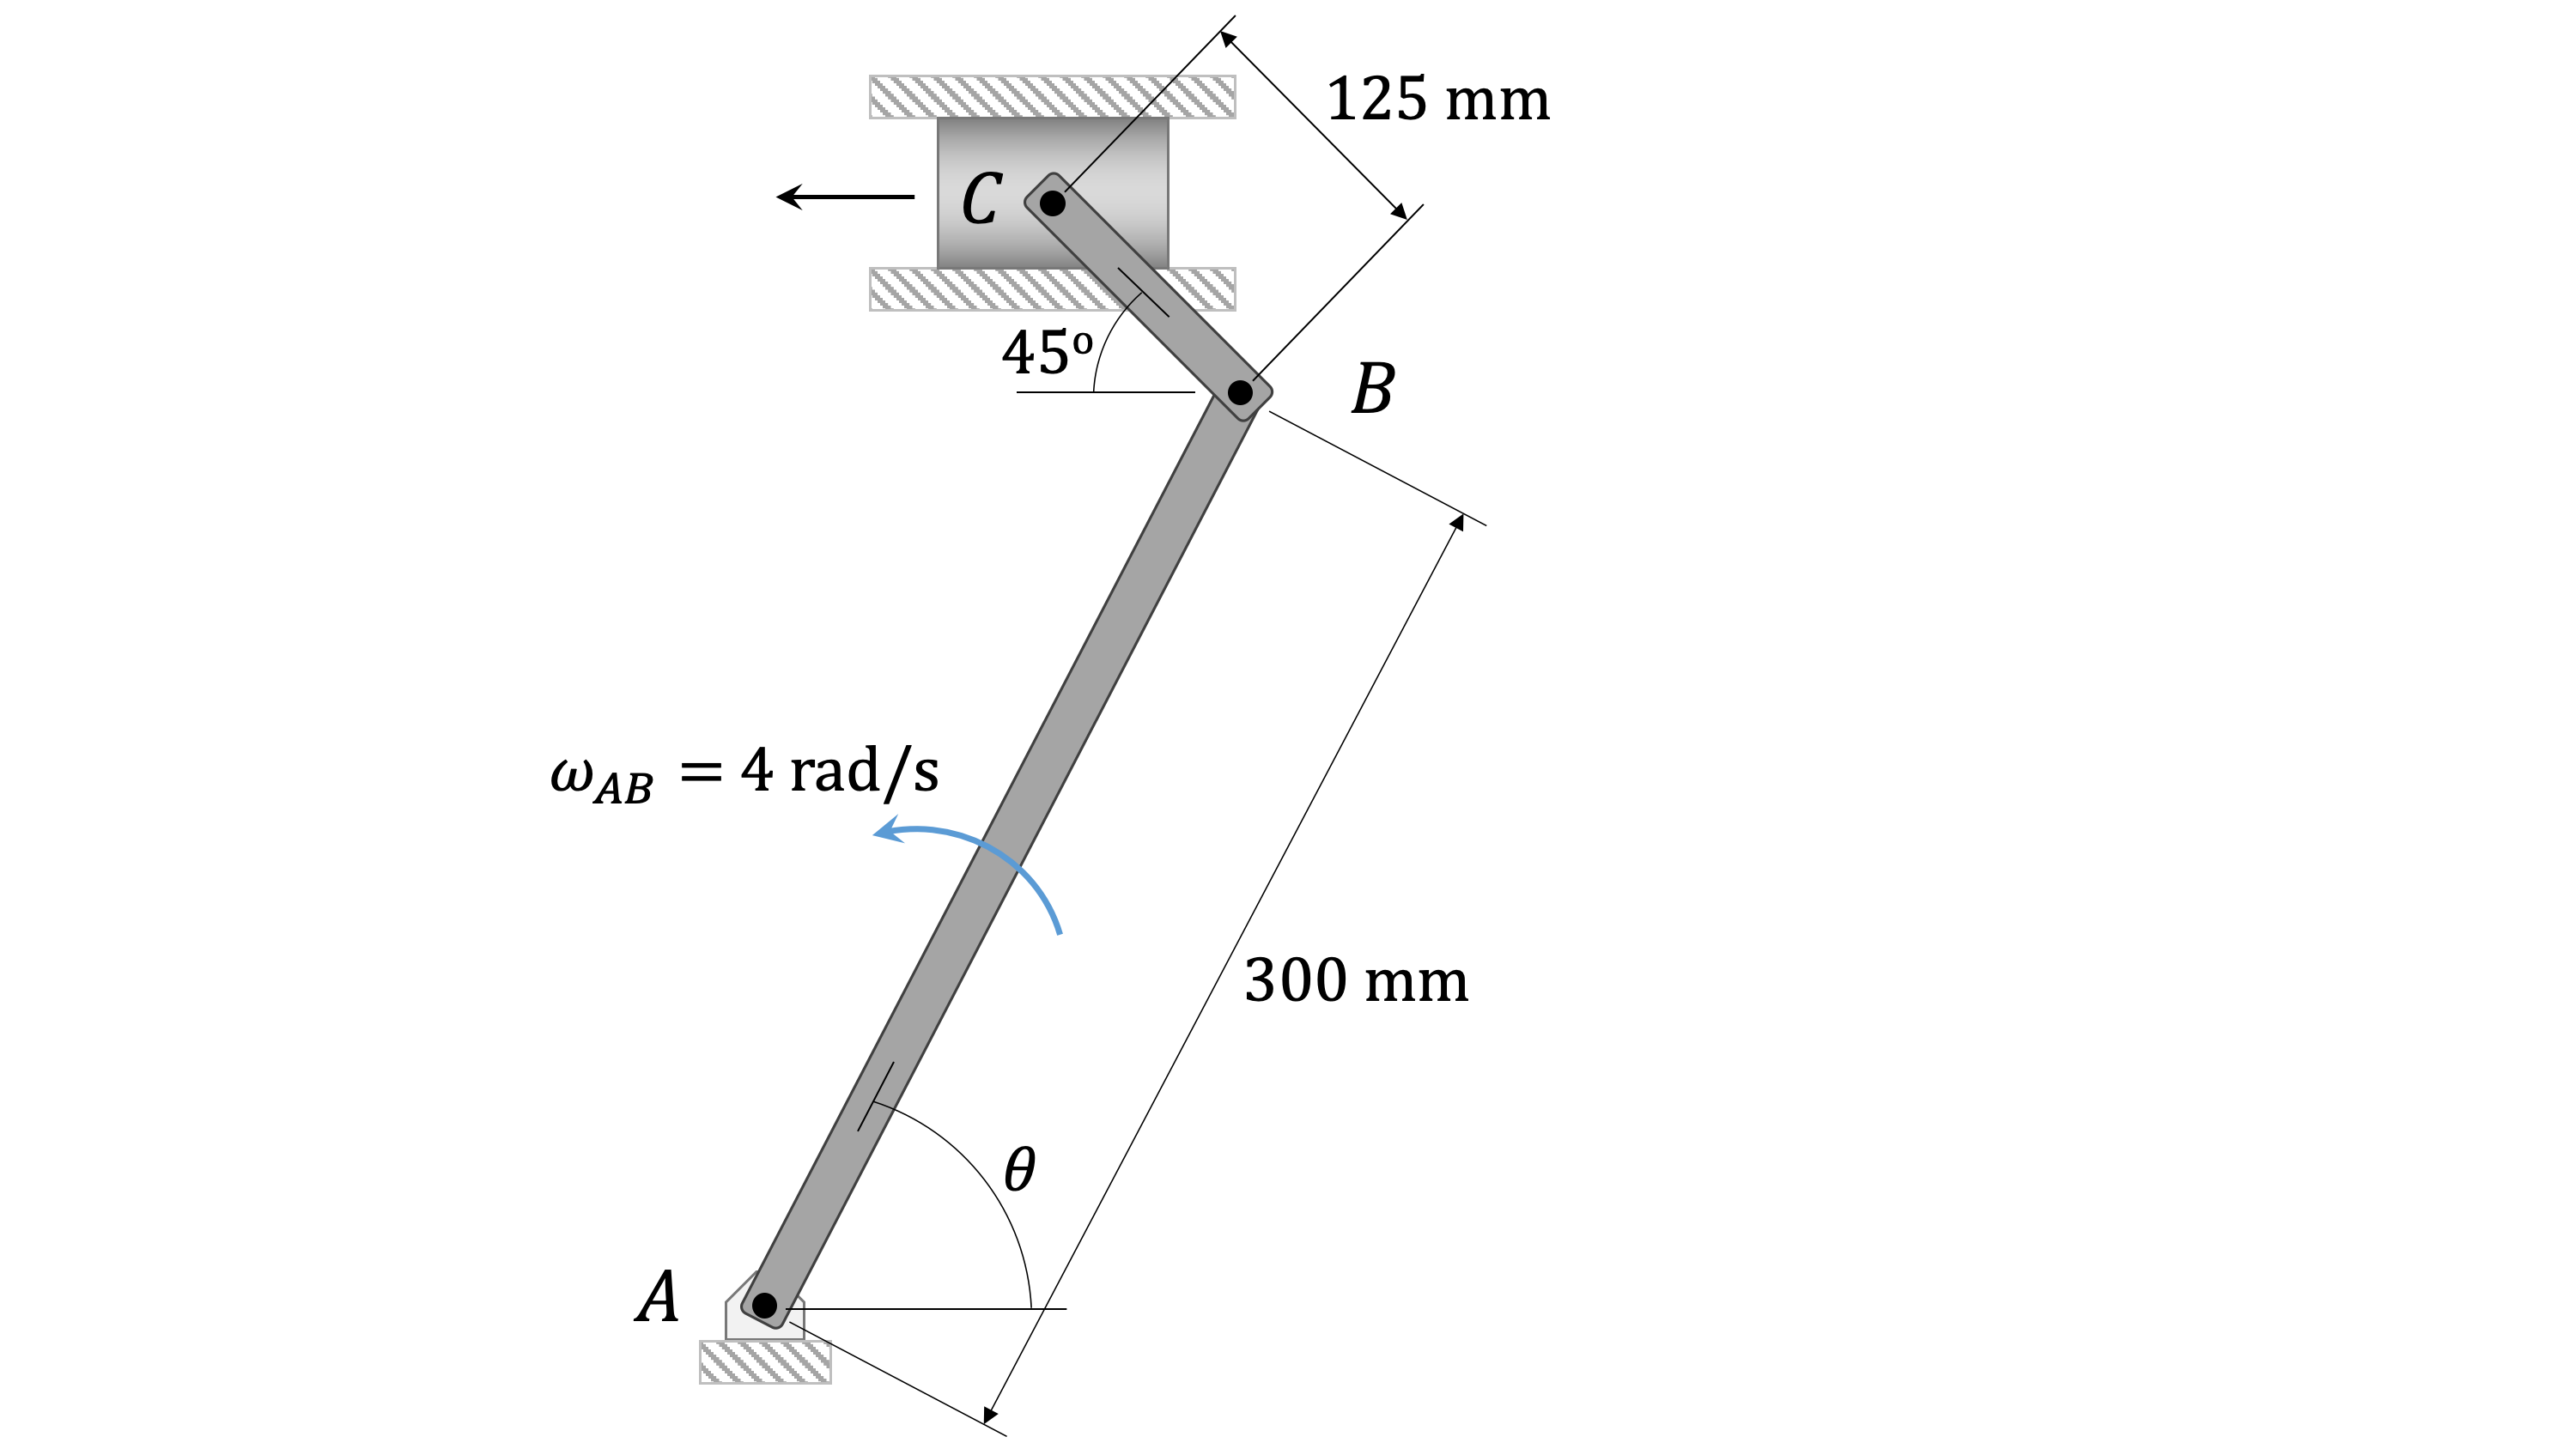
\includegraphics[trim={5cm 0cm 6cm 0cm},clip,width=1\textwidth, center]{Slide15}
\end{minipage}

\newpage

(Example continued)


\chapter{L3: Instantaneous Centres of Zero Velocity}
Readings

\section{Objective}
To be able to identify the ICZV of a rigid body, and to use the ICZV to quickly solve planar motion problems. 

\section{Locating the Instantaneous Centre}
Consider a rigid body that is both translating and rotating.  

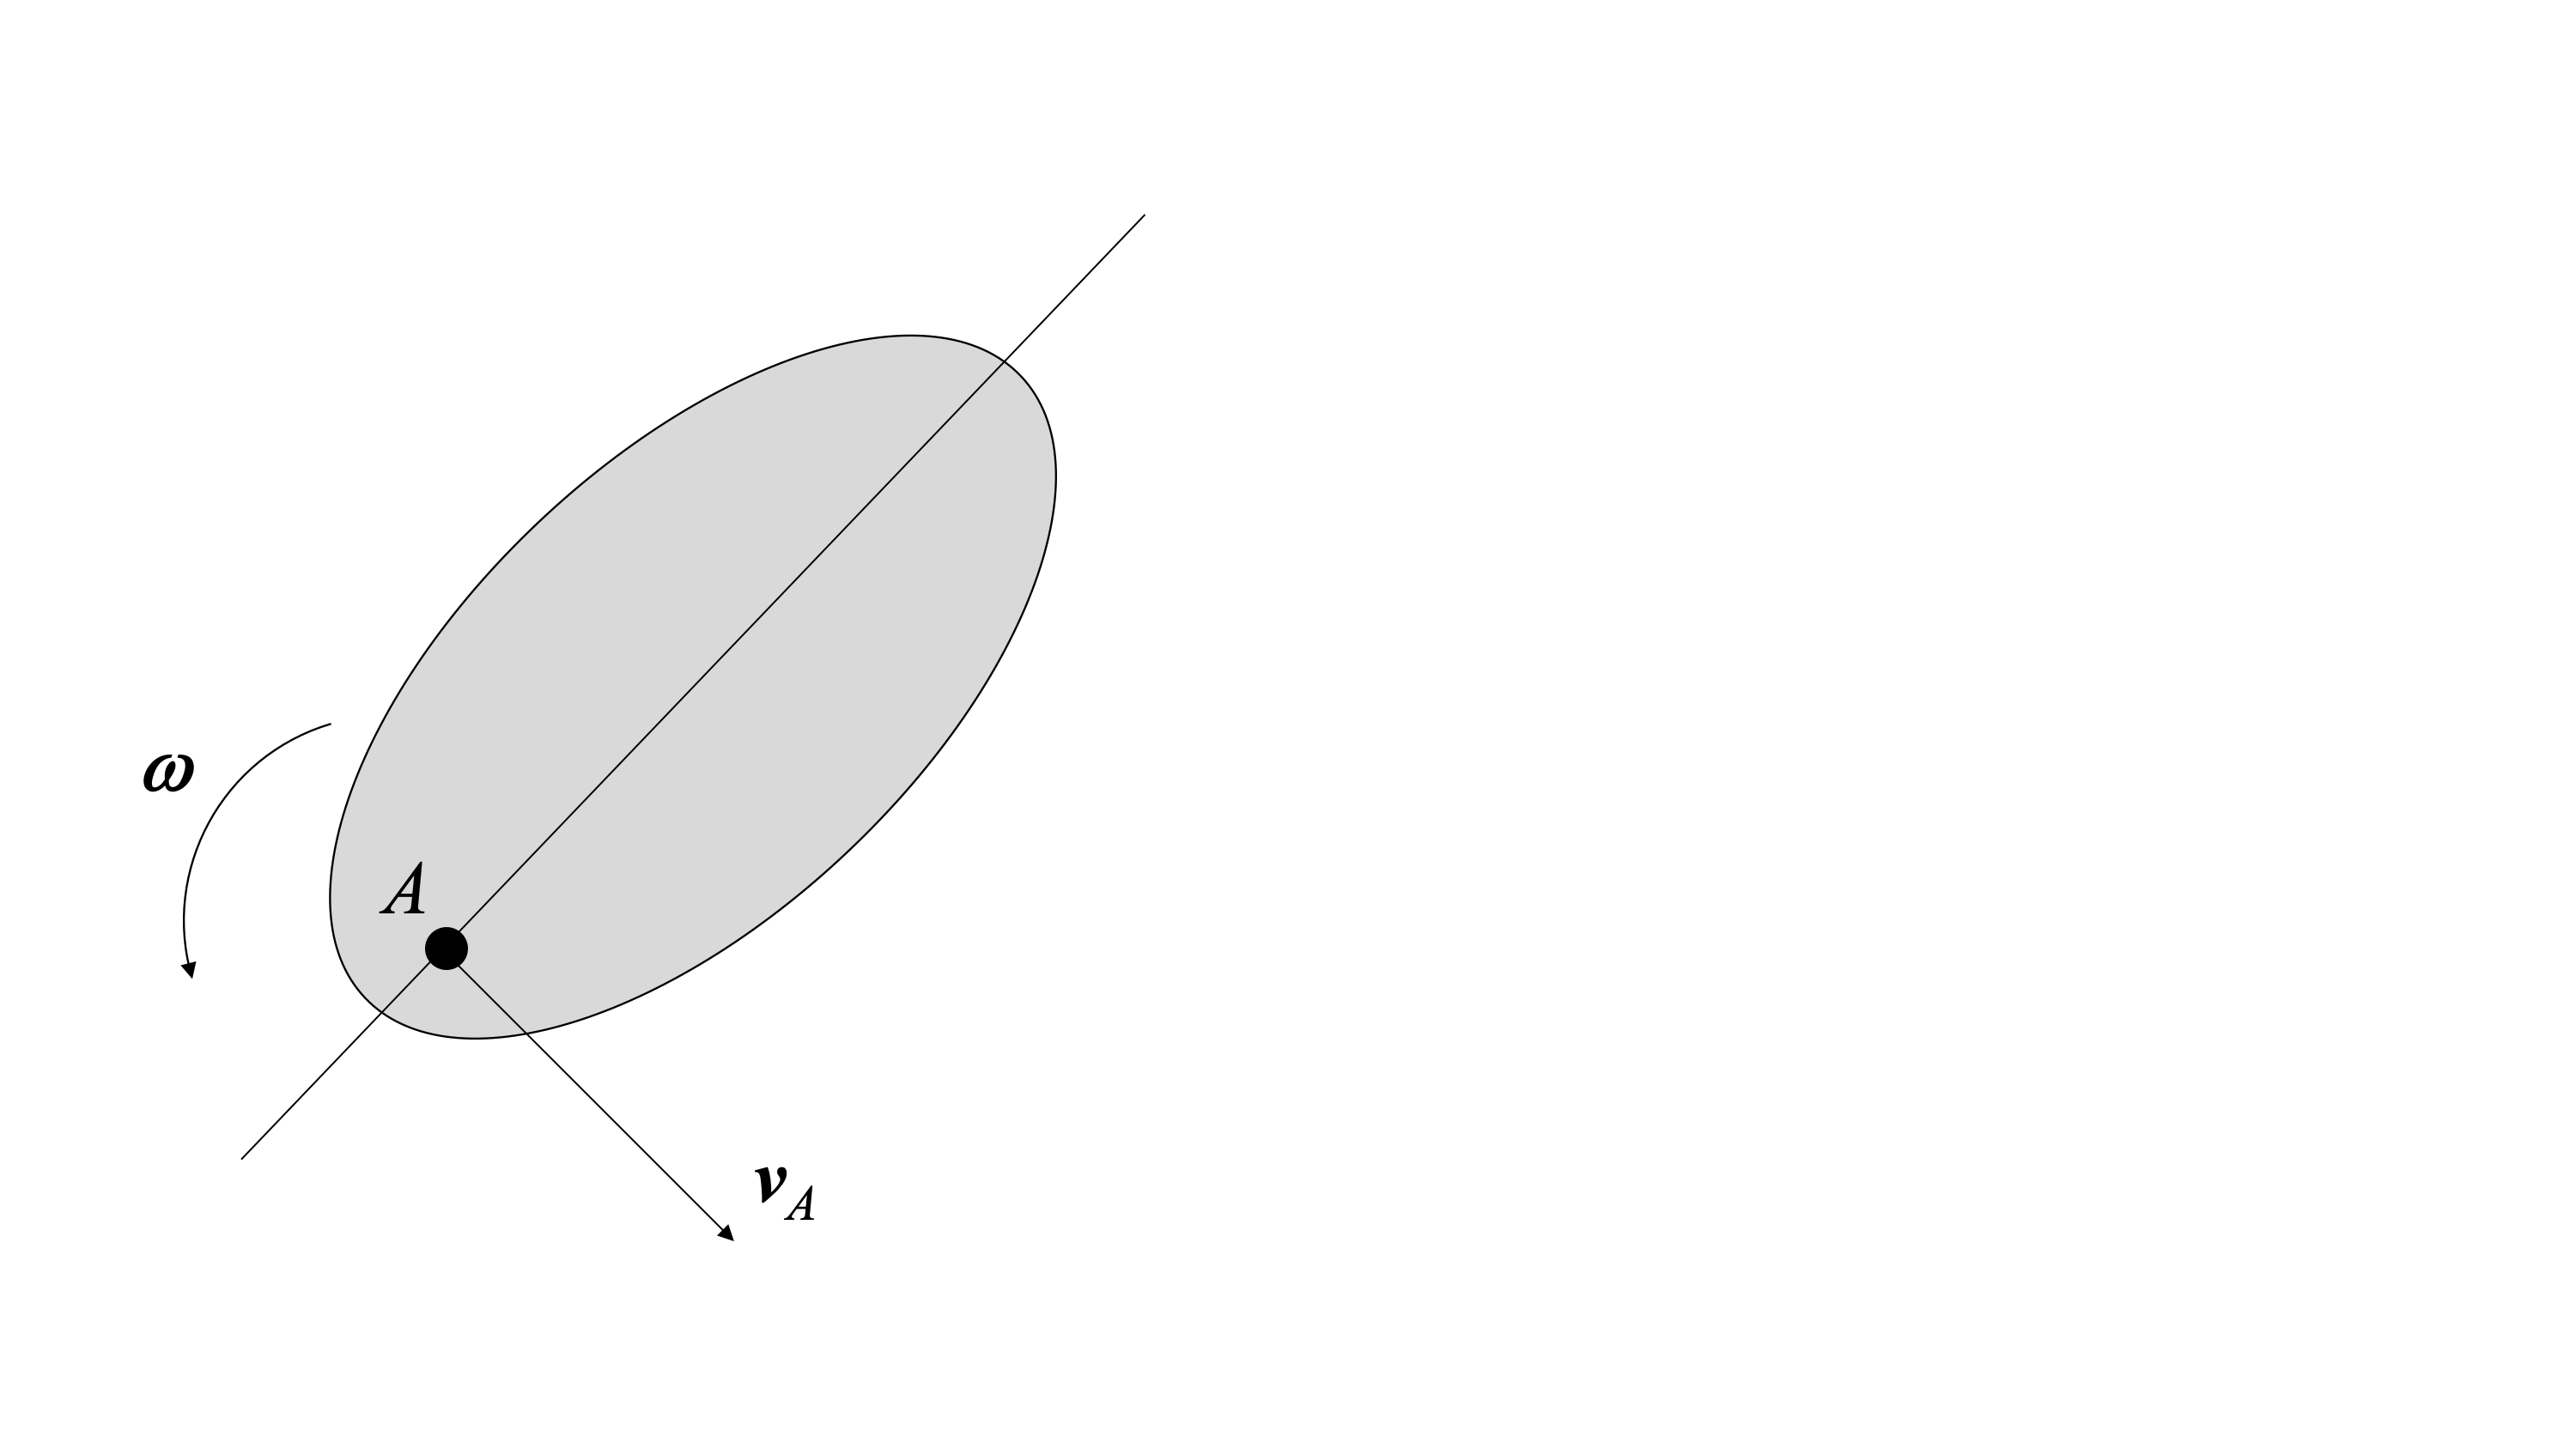
\includegraphics[trim={0cm 2cm 0cm 4cm},clip,width=0.9\textwidth, center]{Slide17}

If we draw a line perpendicular to $\bm{v_A}$ and passing through $A$, all points $P_i$ on this line will have velocity:
\[\bm{v_{P_i}} = \bm{v_A} + \bm{\omega} \times \bm{r_{P_{i}/A}}\]

If we set up a coordinate system at point $A$ with $x$ along $\bm{v_A}$ and $y$ along the line perpendicular to $\bm{v_A}$, then:

\-\hspace{1cm} $\bm{v_A} = $

\-\hspace{1cm} $\bm{\omega} = $

\-\hspace{1cm} $\bm{r_{P_{i}/A}} = $

\newpage
Now: $\bm{v_{P_i}} = v_A \bm{\hat{i}} + \omega \bm{\hat{k}} \times (A P_i) \bm{\hat{j}}$

\-\hspace{1cm} $\bm{v_{P_i}} =$

\vspace*{2\baselineskip}

Therefore, all points $P_i$ on a line perpendicular to $\bm{v_A}$, passing through $A$, have velocity in the SAME DIRECTION as $\bm{v_A}$.  

\vspace*{2\baselineskip}

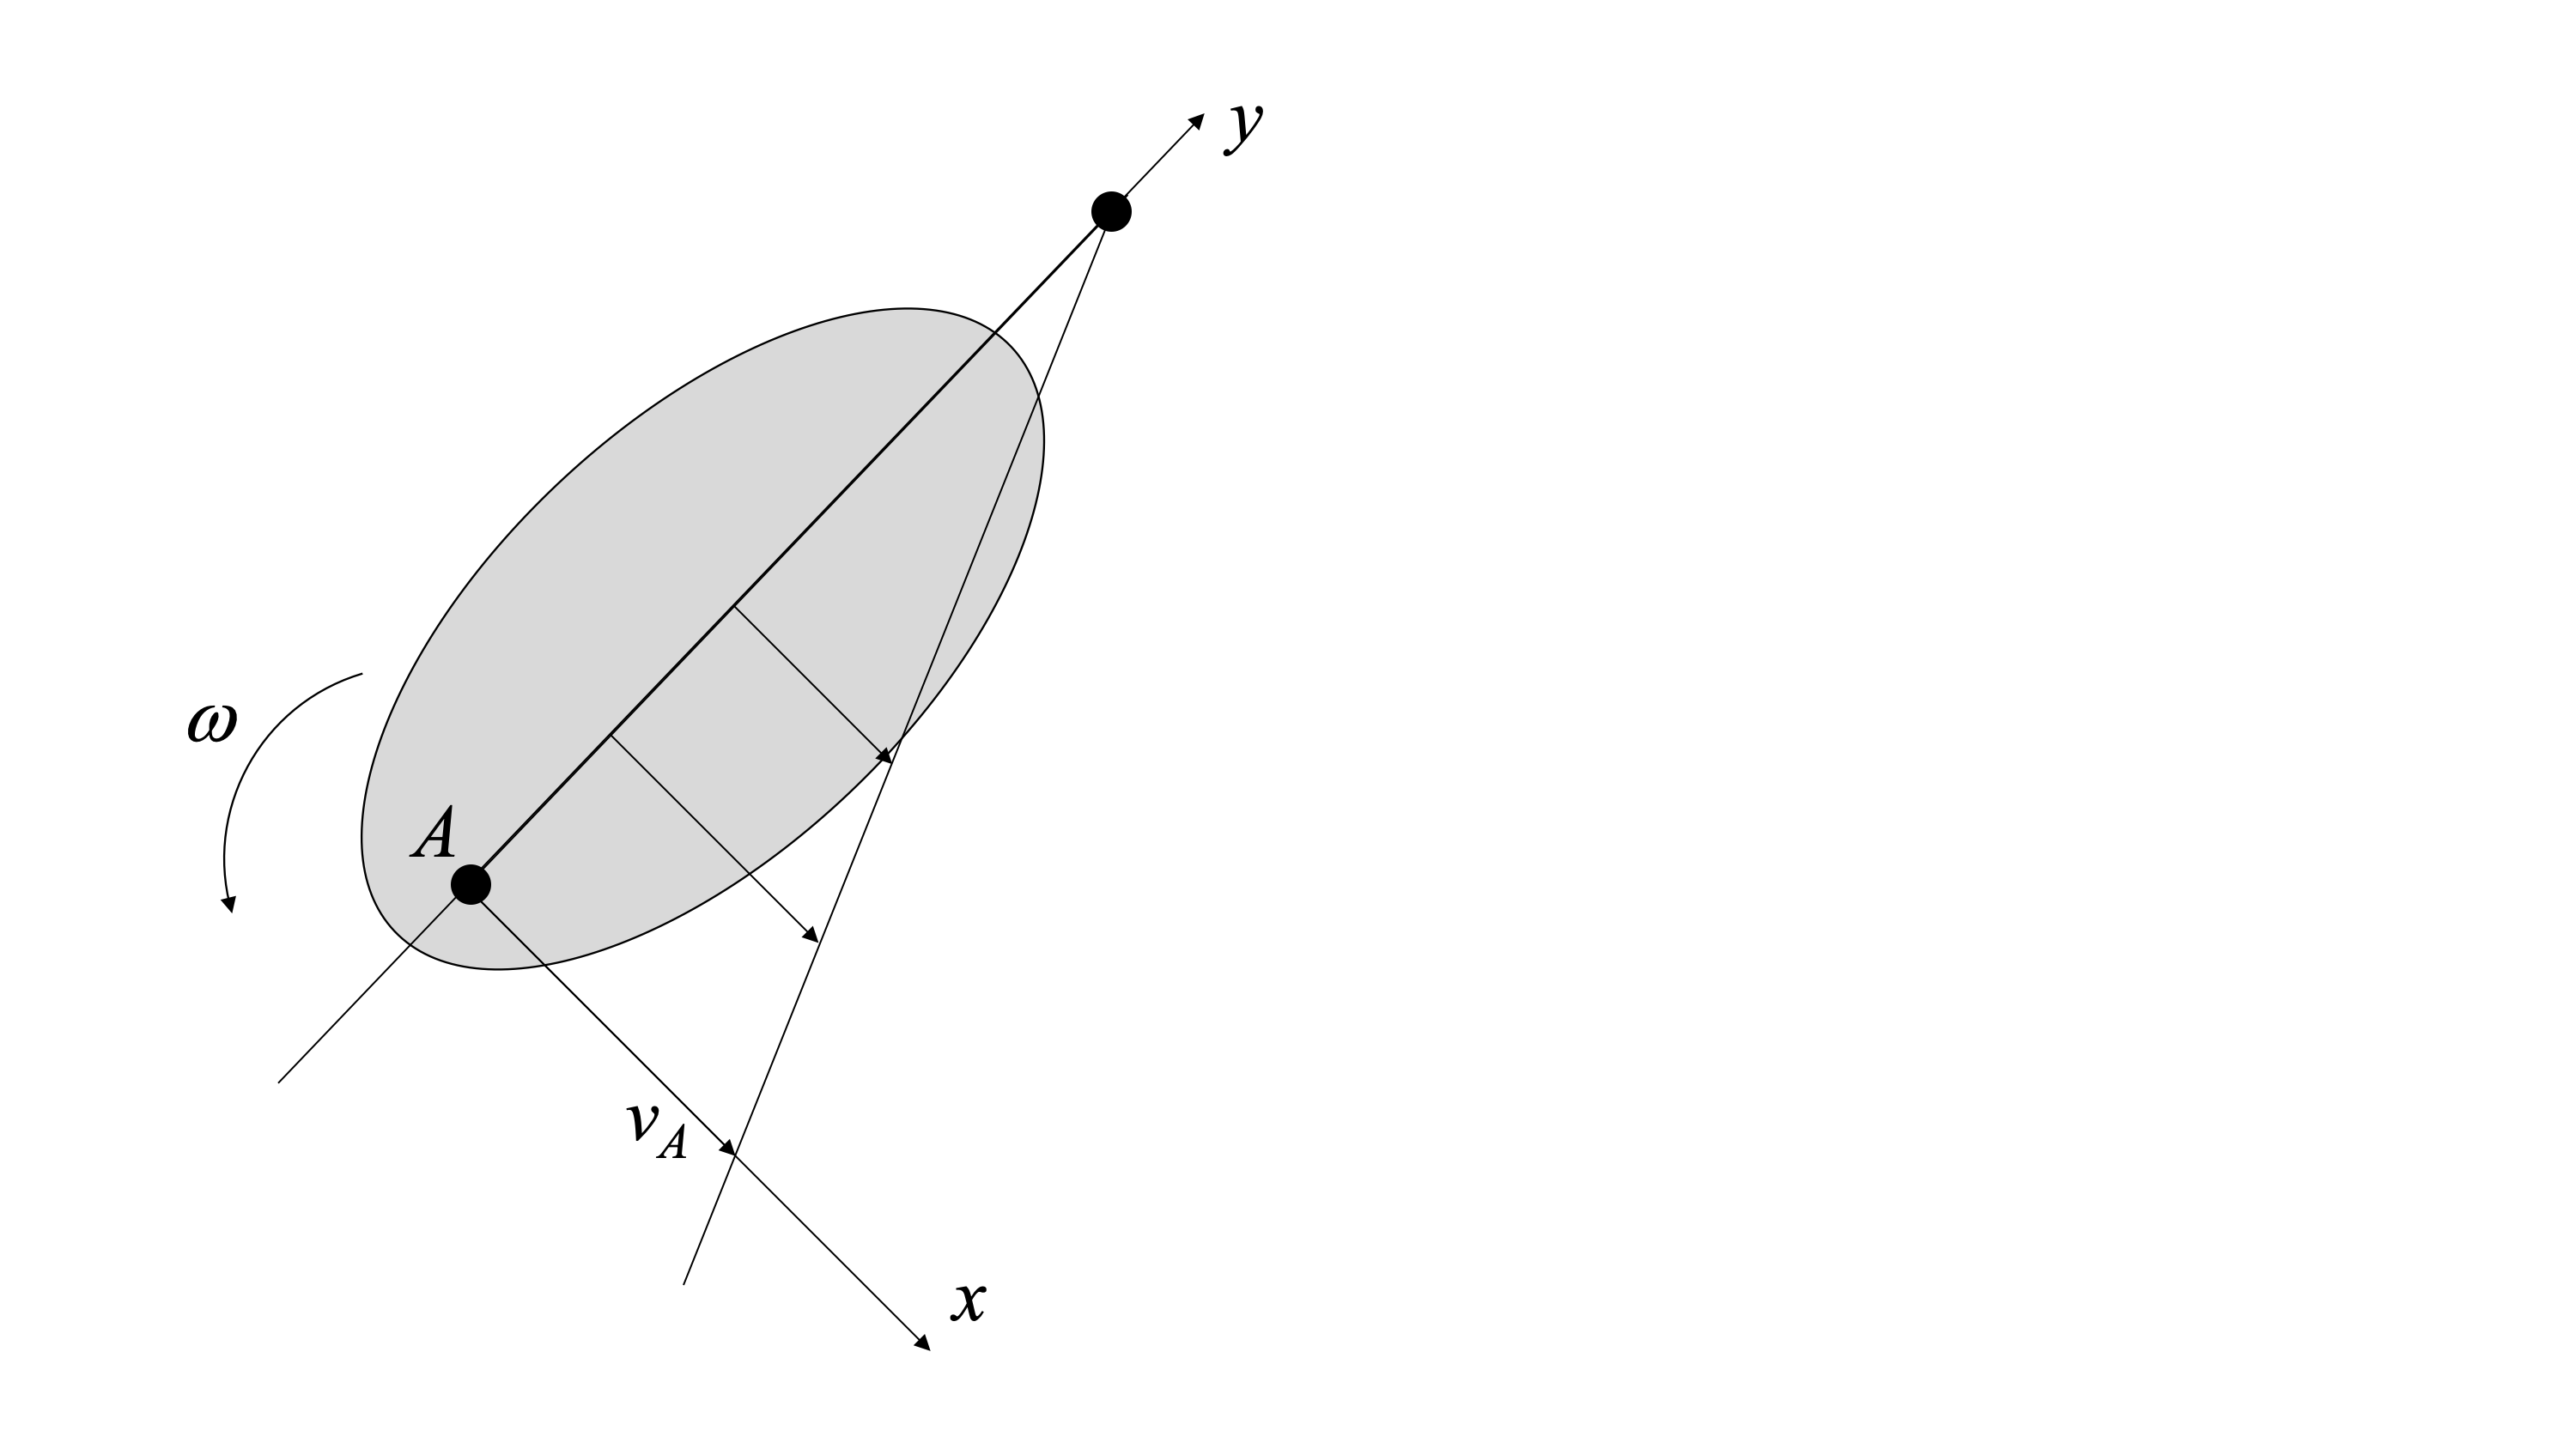
\includegraphics[trim={0cm 0cm 0cm 0cm},clip,width=0.9\textwidth, center]{Slide18}

At some point along the line $P^{*}$, ${AP^{*}} \omega = v_A$

At this point, $v_{P^{*}}= v_A - (AP^{*}) \omega=0$

This point is known as the \textbf{Instantaneous Centre of Zero Velocity, or ICZV}. 

\newpage
\section{Comments about the ICZV}
\begin{itemize}
\item The ICZV is always on a line passing through any point, $P$, on the body that is perpendicular to the absolute velocity of point $P$, $\bm{P}$. 

\vspace*{2\baselineskip}

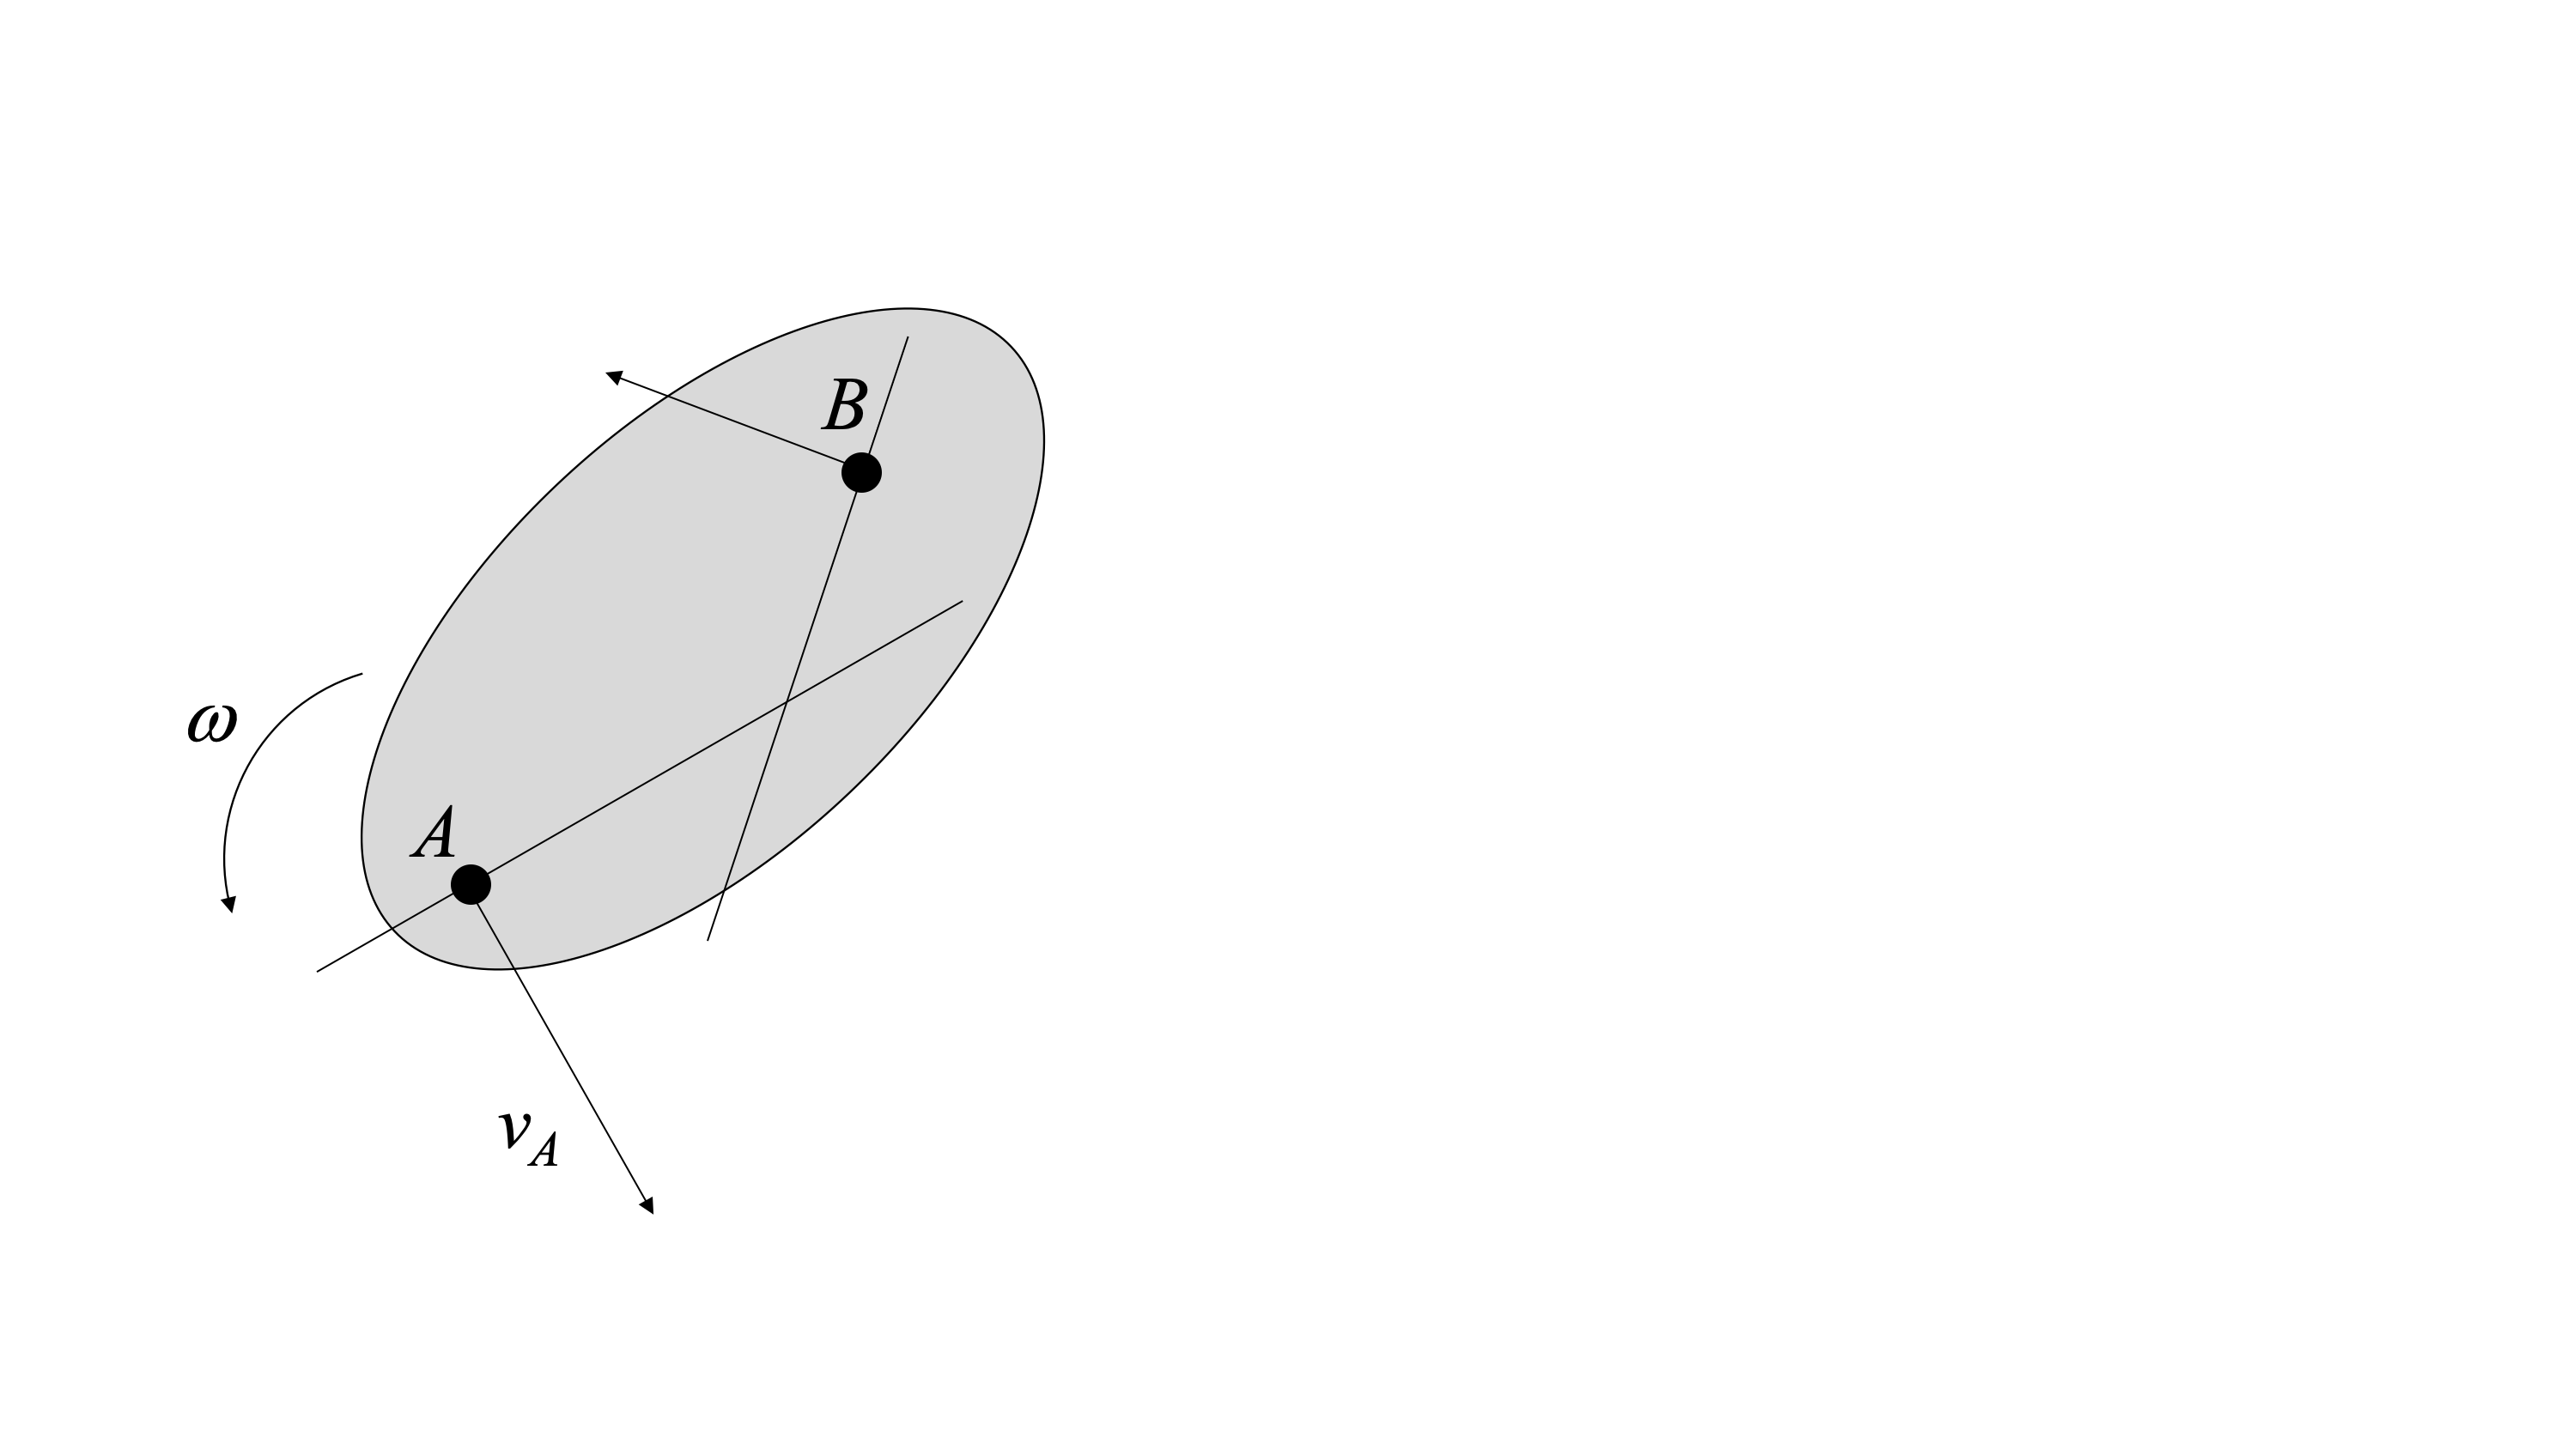
\includegraphics[trim={0cm 2cm 0cm 4cm},clip,width=0.9\textwidth, center]{Slide19}

\item The ICZV is NOT necessarily located on the body!

\vspace*{2\baselineskip}

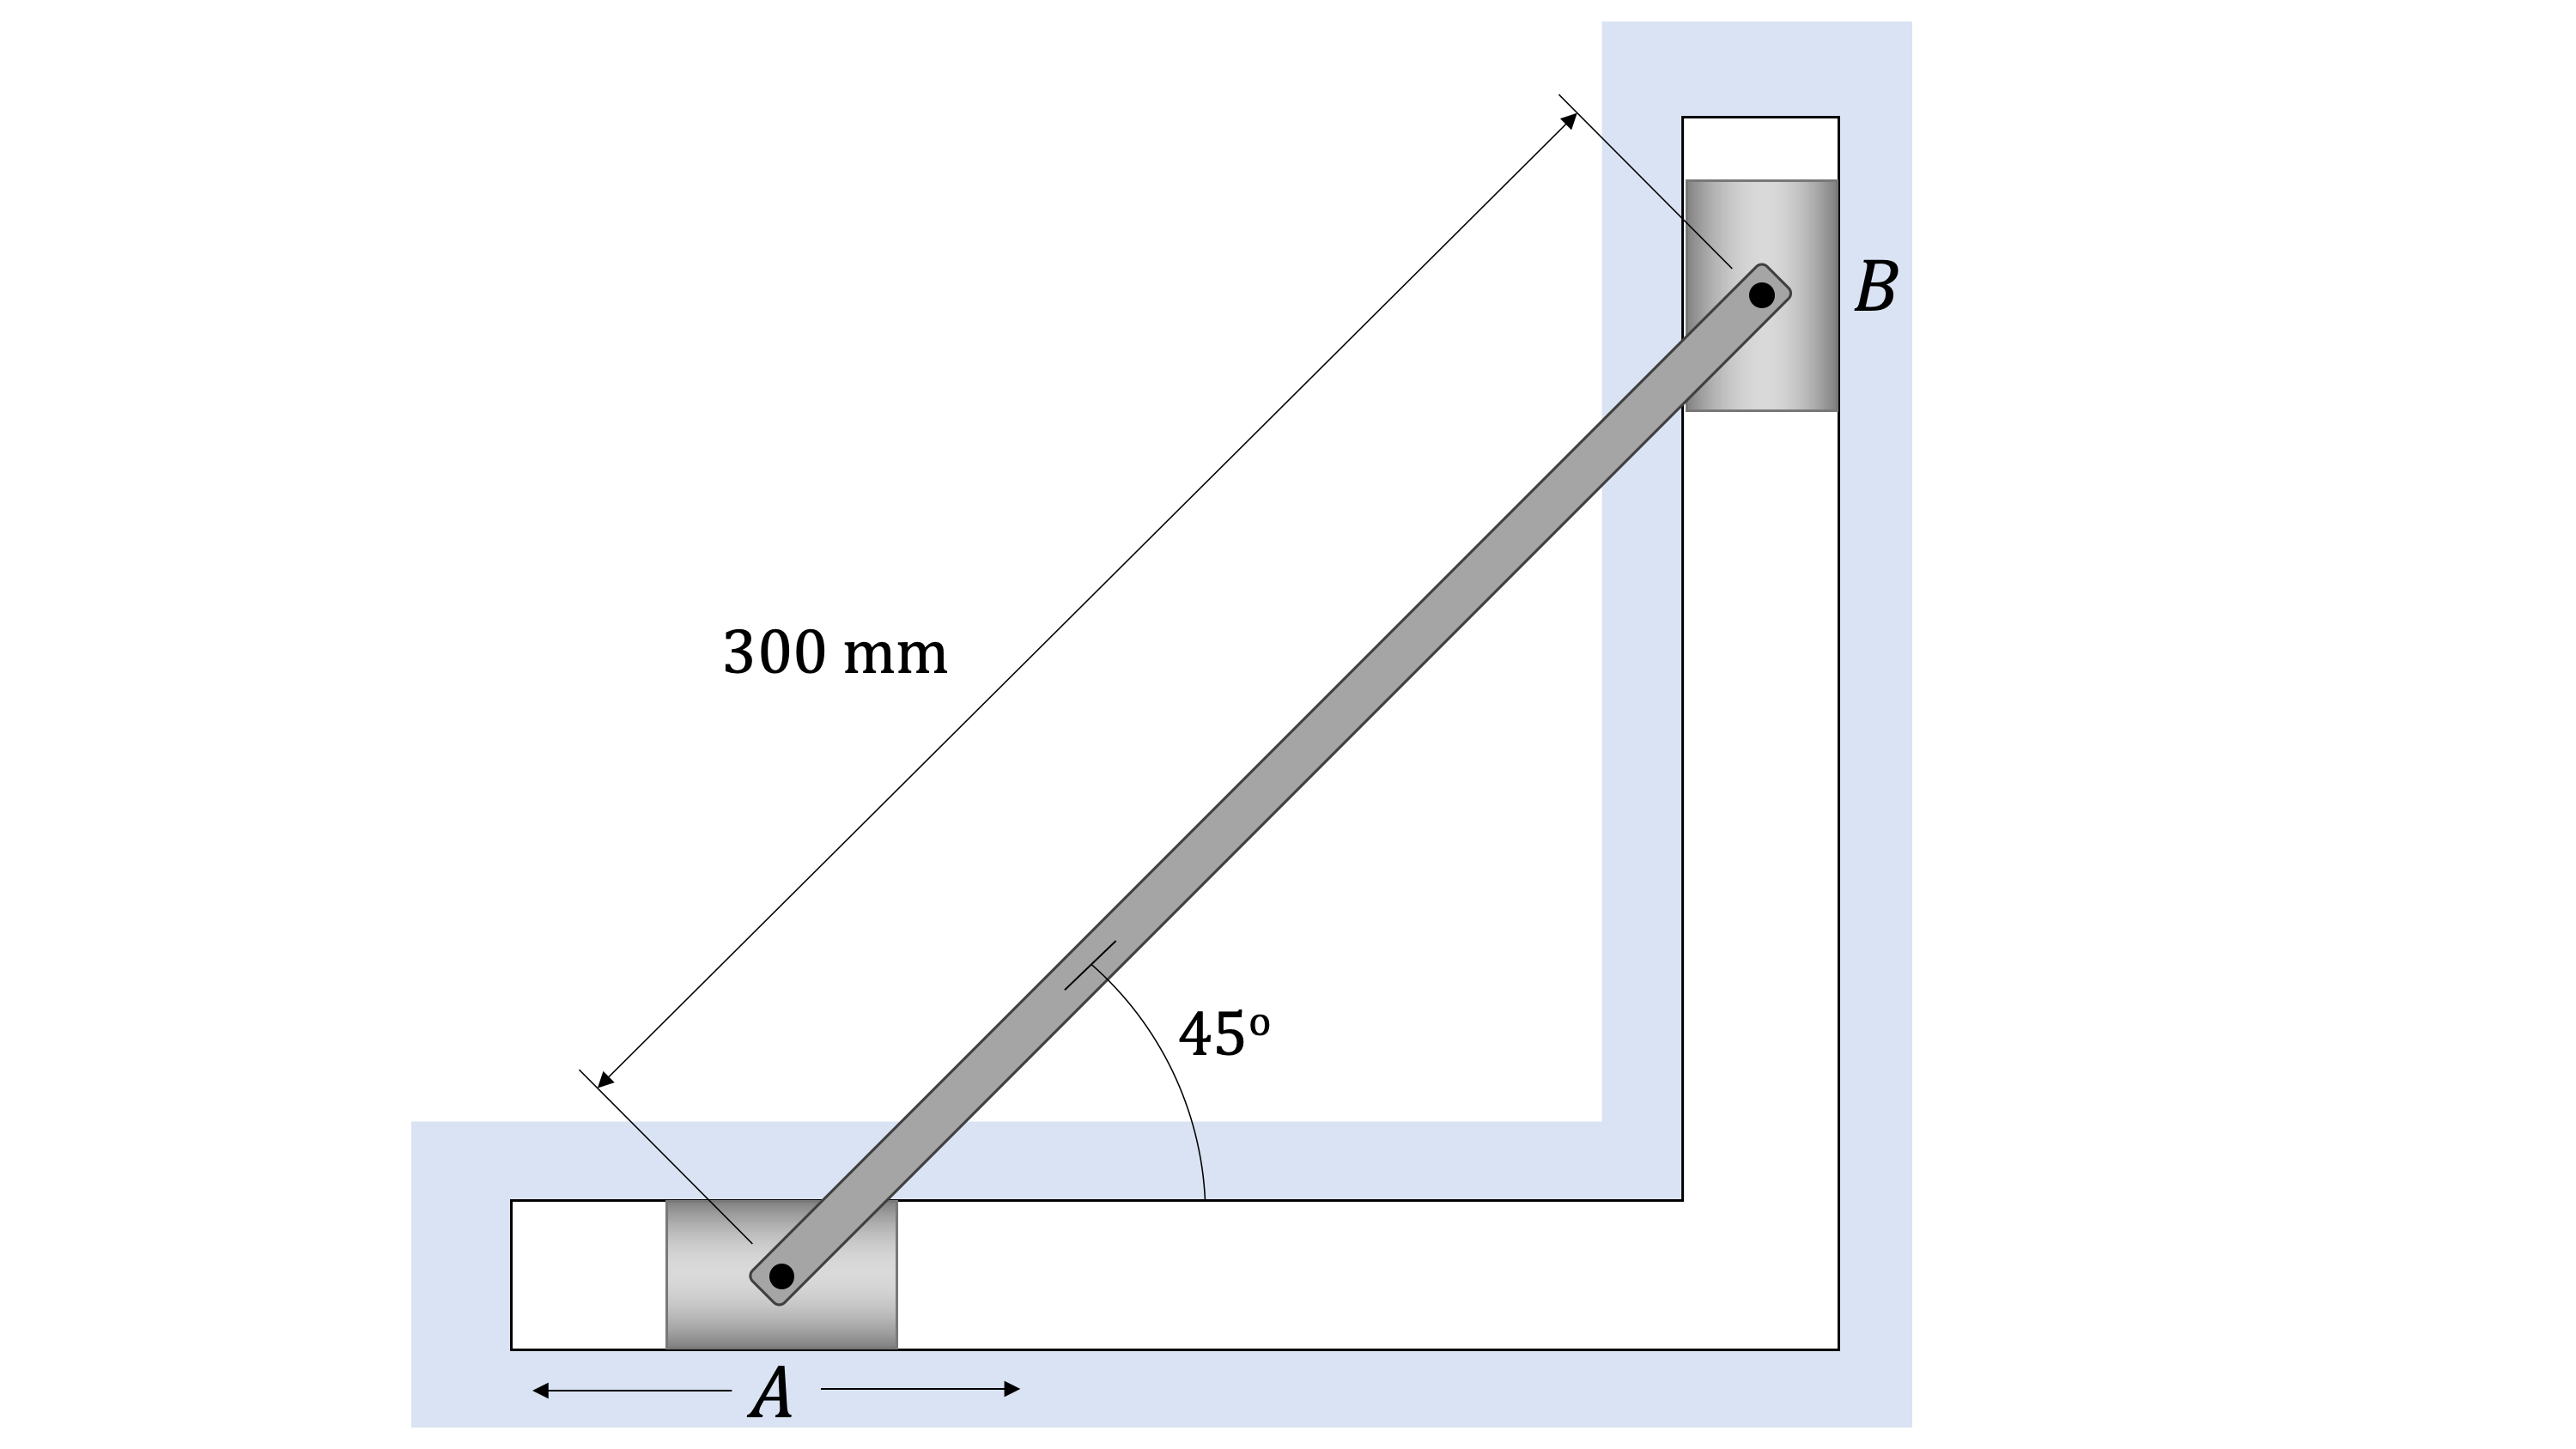
\includegraphics[trim={0cm 0cm 0cm 0cm},clip,width=0.7\textwidth, center]{Slide20}

\newpage
\item For general plane motion (translation plus rotation), the location of the ICZV changes over time. 

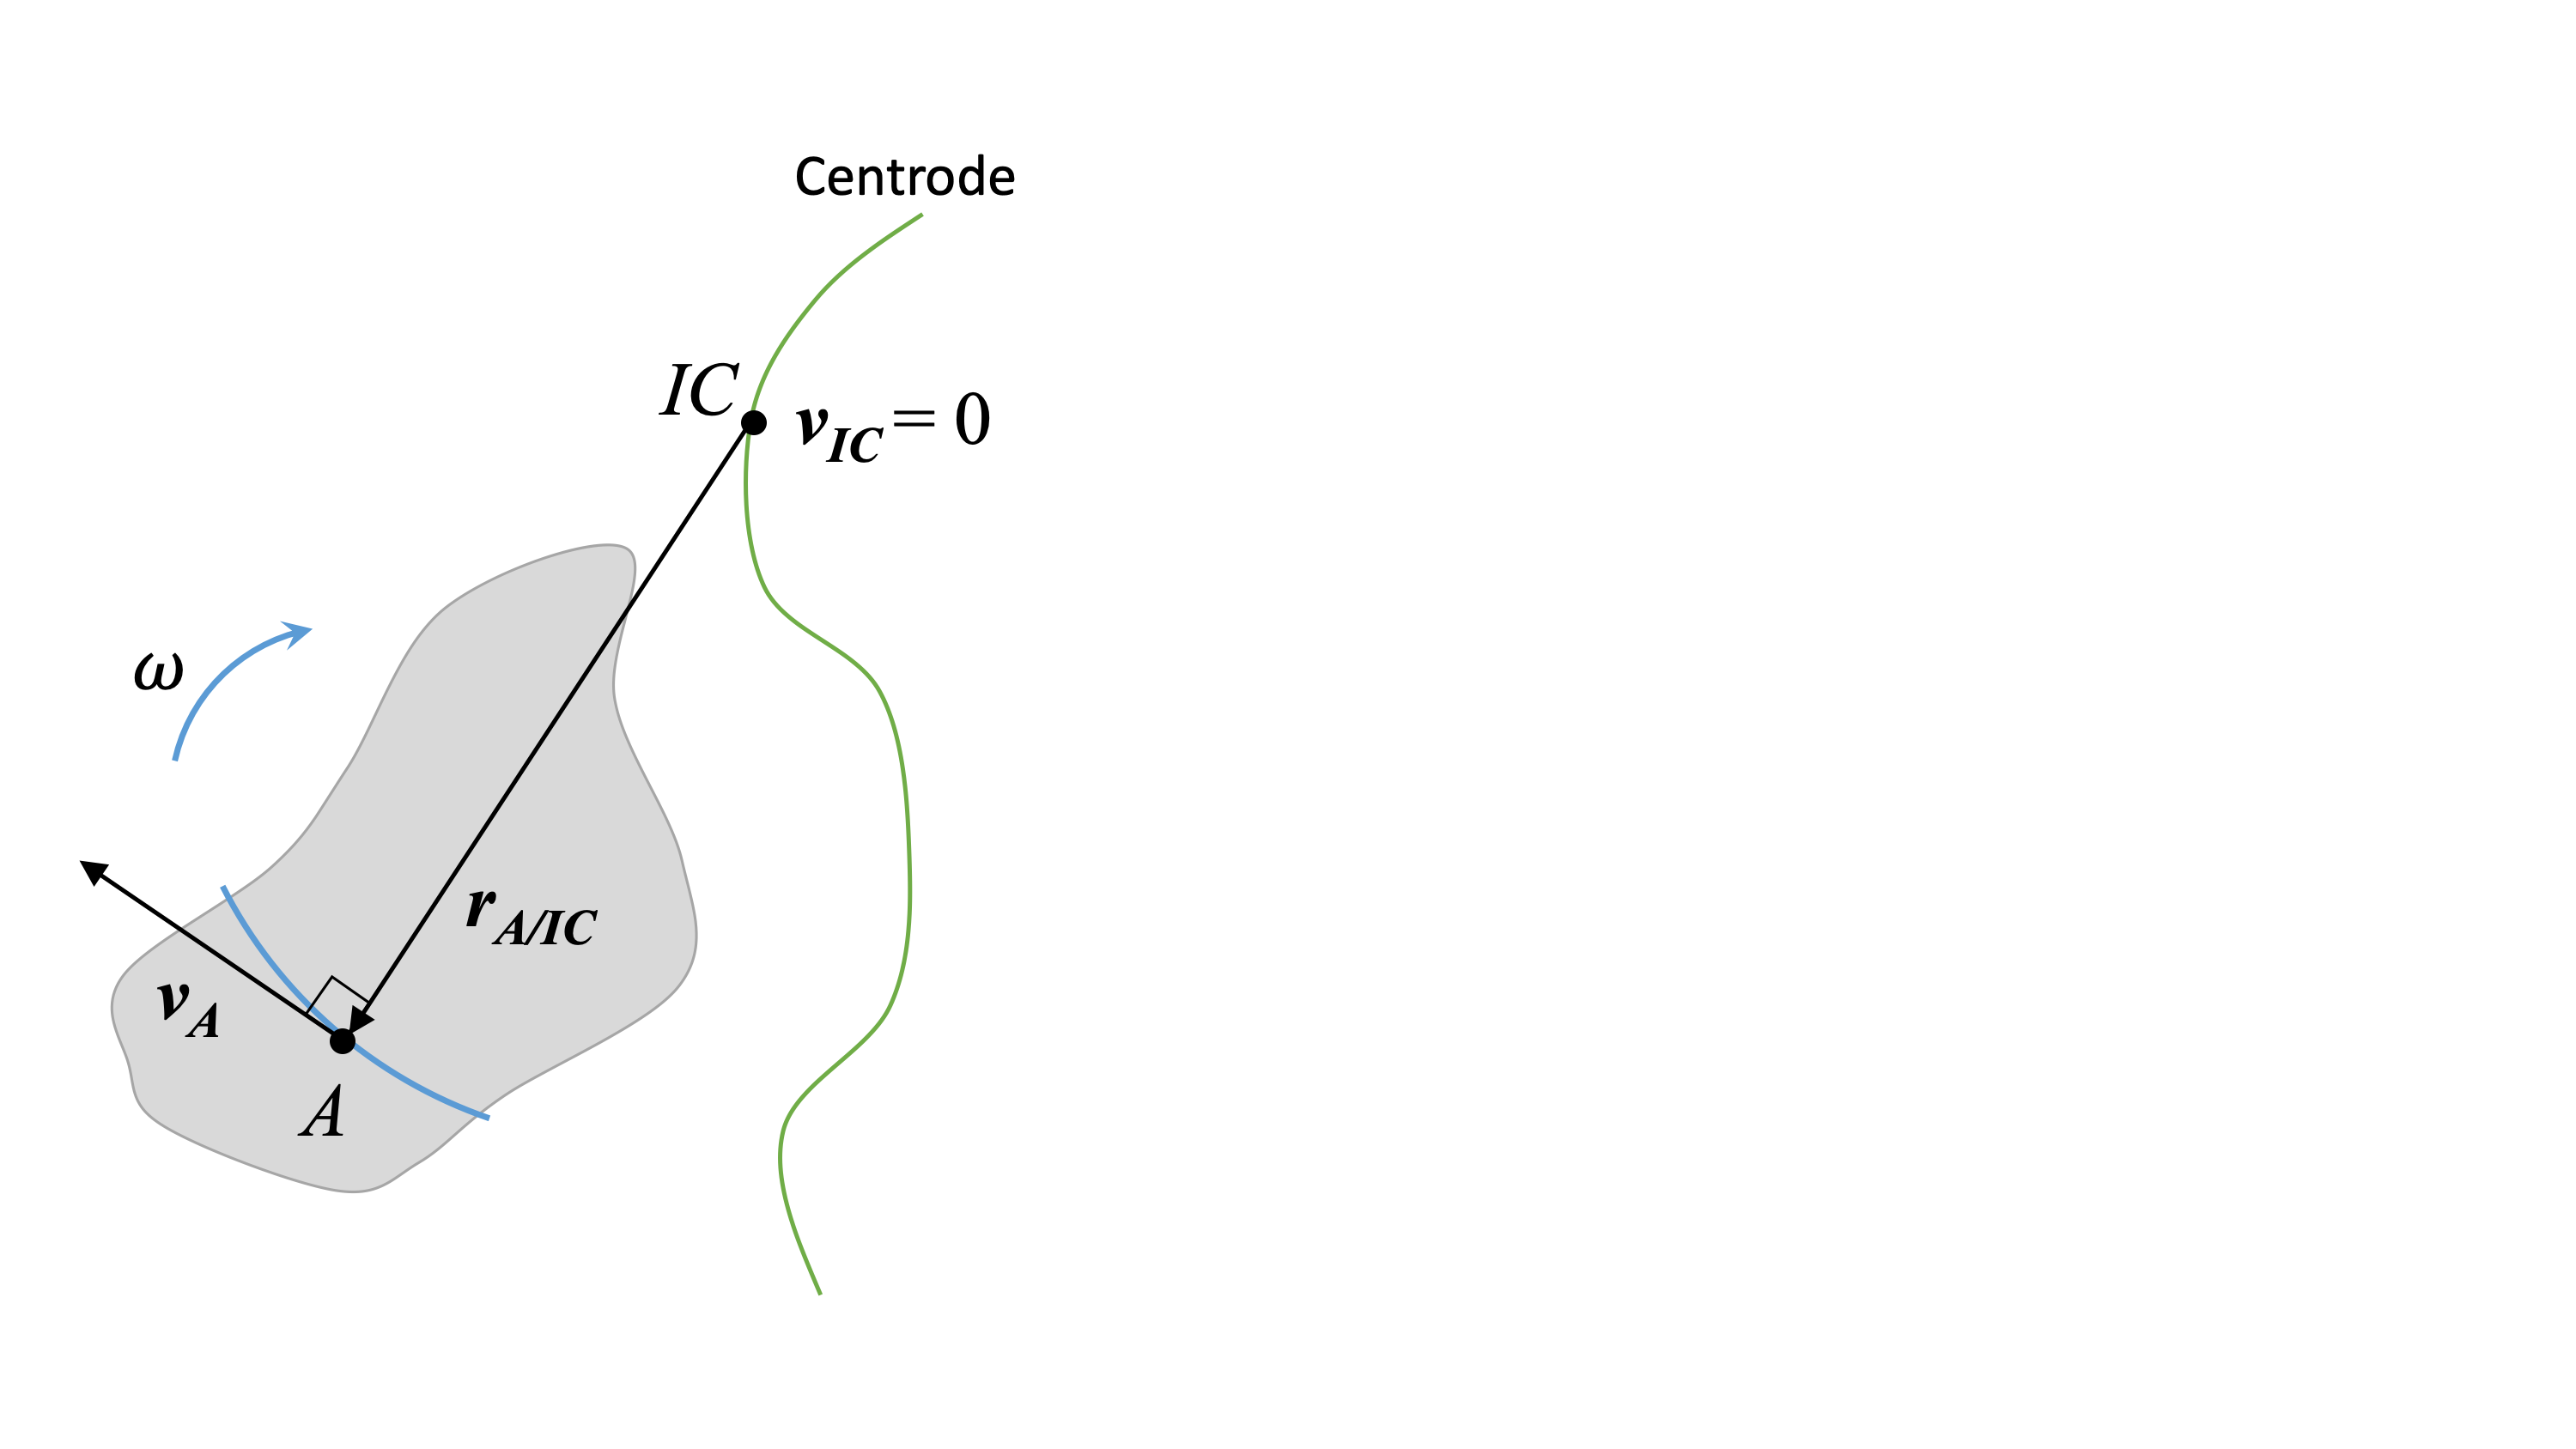
\includegraphics[trim={0cm 1cm 14cm 1cm},clip,width=0.5\textwidth, center]{Slide21}

\item For bodies that are \textbf{pinned to a fixed location}, the ICZV is at the pin. \\


\begin{minipage}[c]{0.3\textwidth}
\begin{tabular}{  c  }
$v_B = \omega r_{B/A}$ \\
  \\
$v_P = \omega r_{P/A}$\\
 \\
$\displaystyle \frac{v_P}{v_B} = \frac{r_{P/A}}{r_{B/A}}$ \\
 \\
\end{tabular}
\label{tab:singlebest}
\end{minipage}%%%
\begin{minipage}[c]{0.8\textwidth}
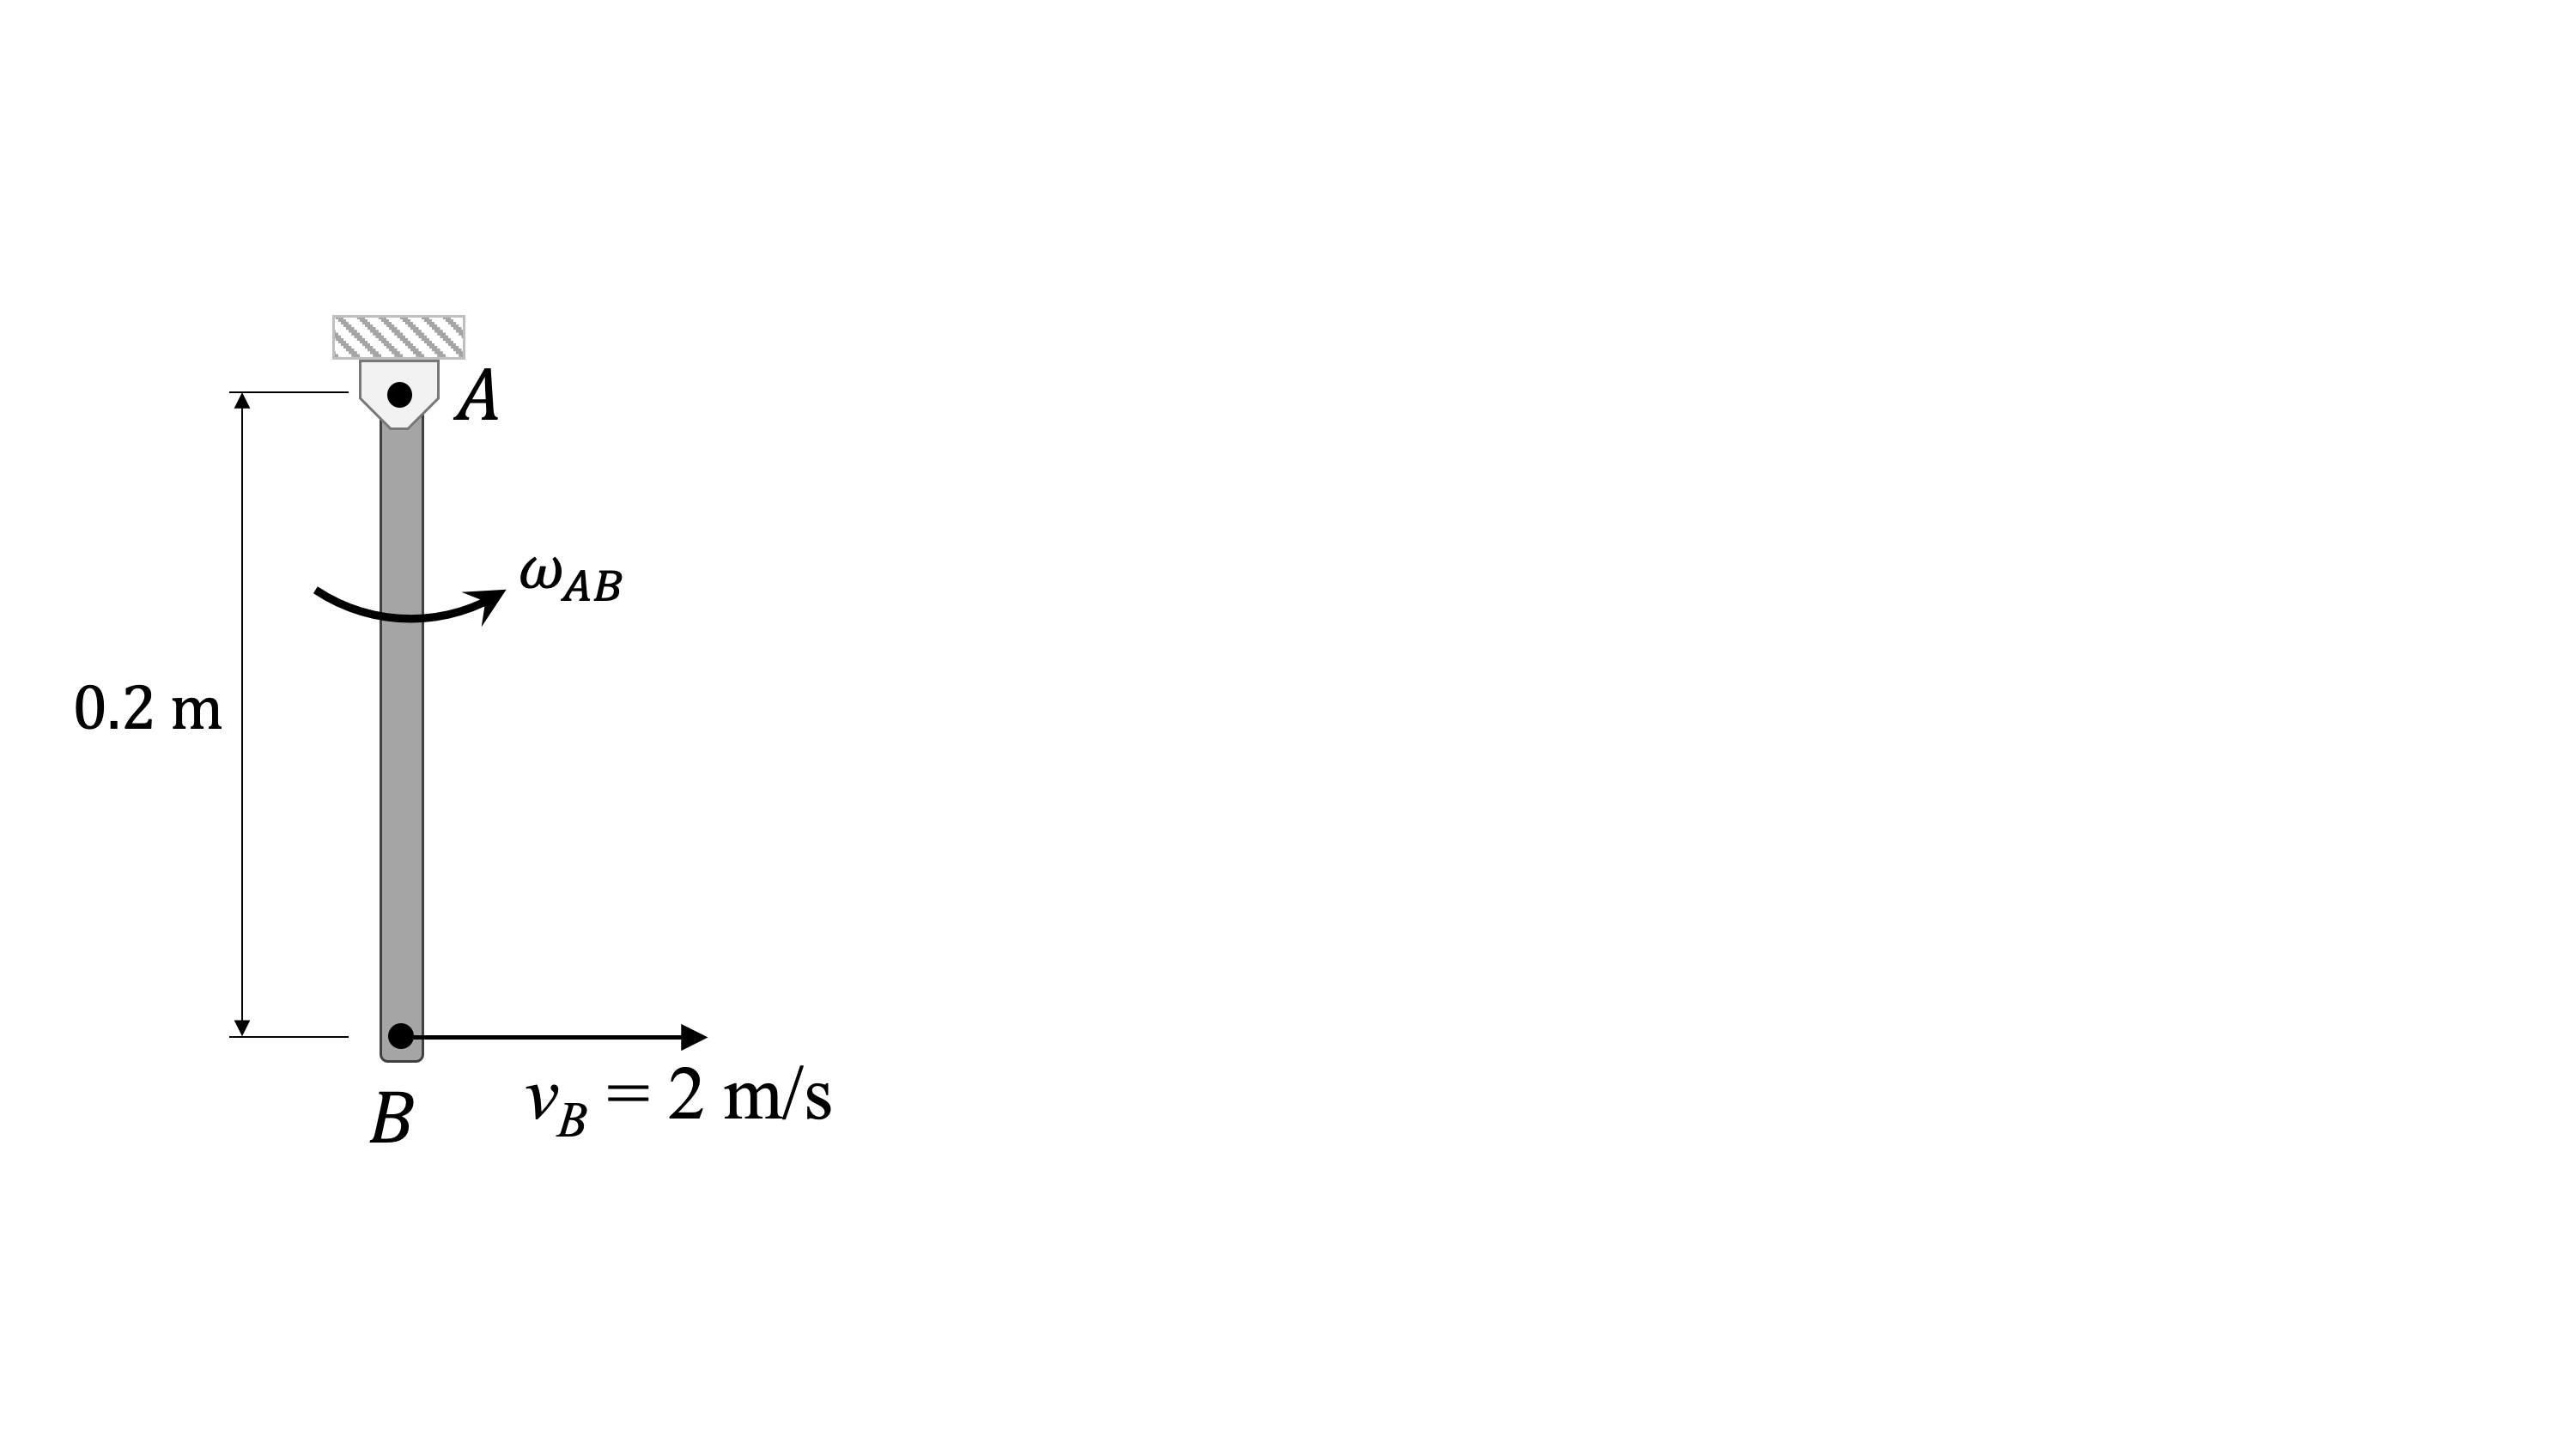
\includegraphics[trim={0cm 2cm 18cm 2cm},clip,width=0.45\textwidth, center]{Slide22} 
\end{minipage}

\newpage
\item If the location of the ICZV is known, the velocity of any other point, $P$, on the body is: \\
\[ \bm{v_P} = \bm{\omega} \times \bm{r_{P/ICZV}} \]

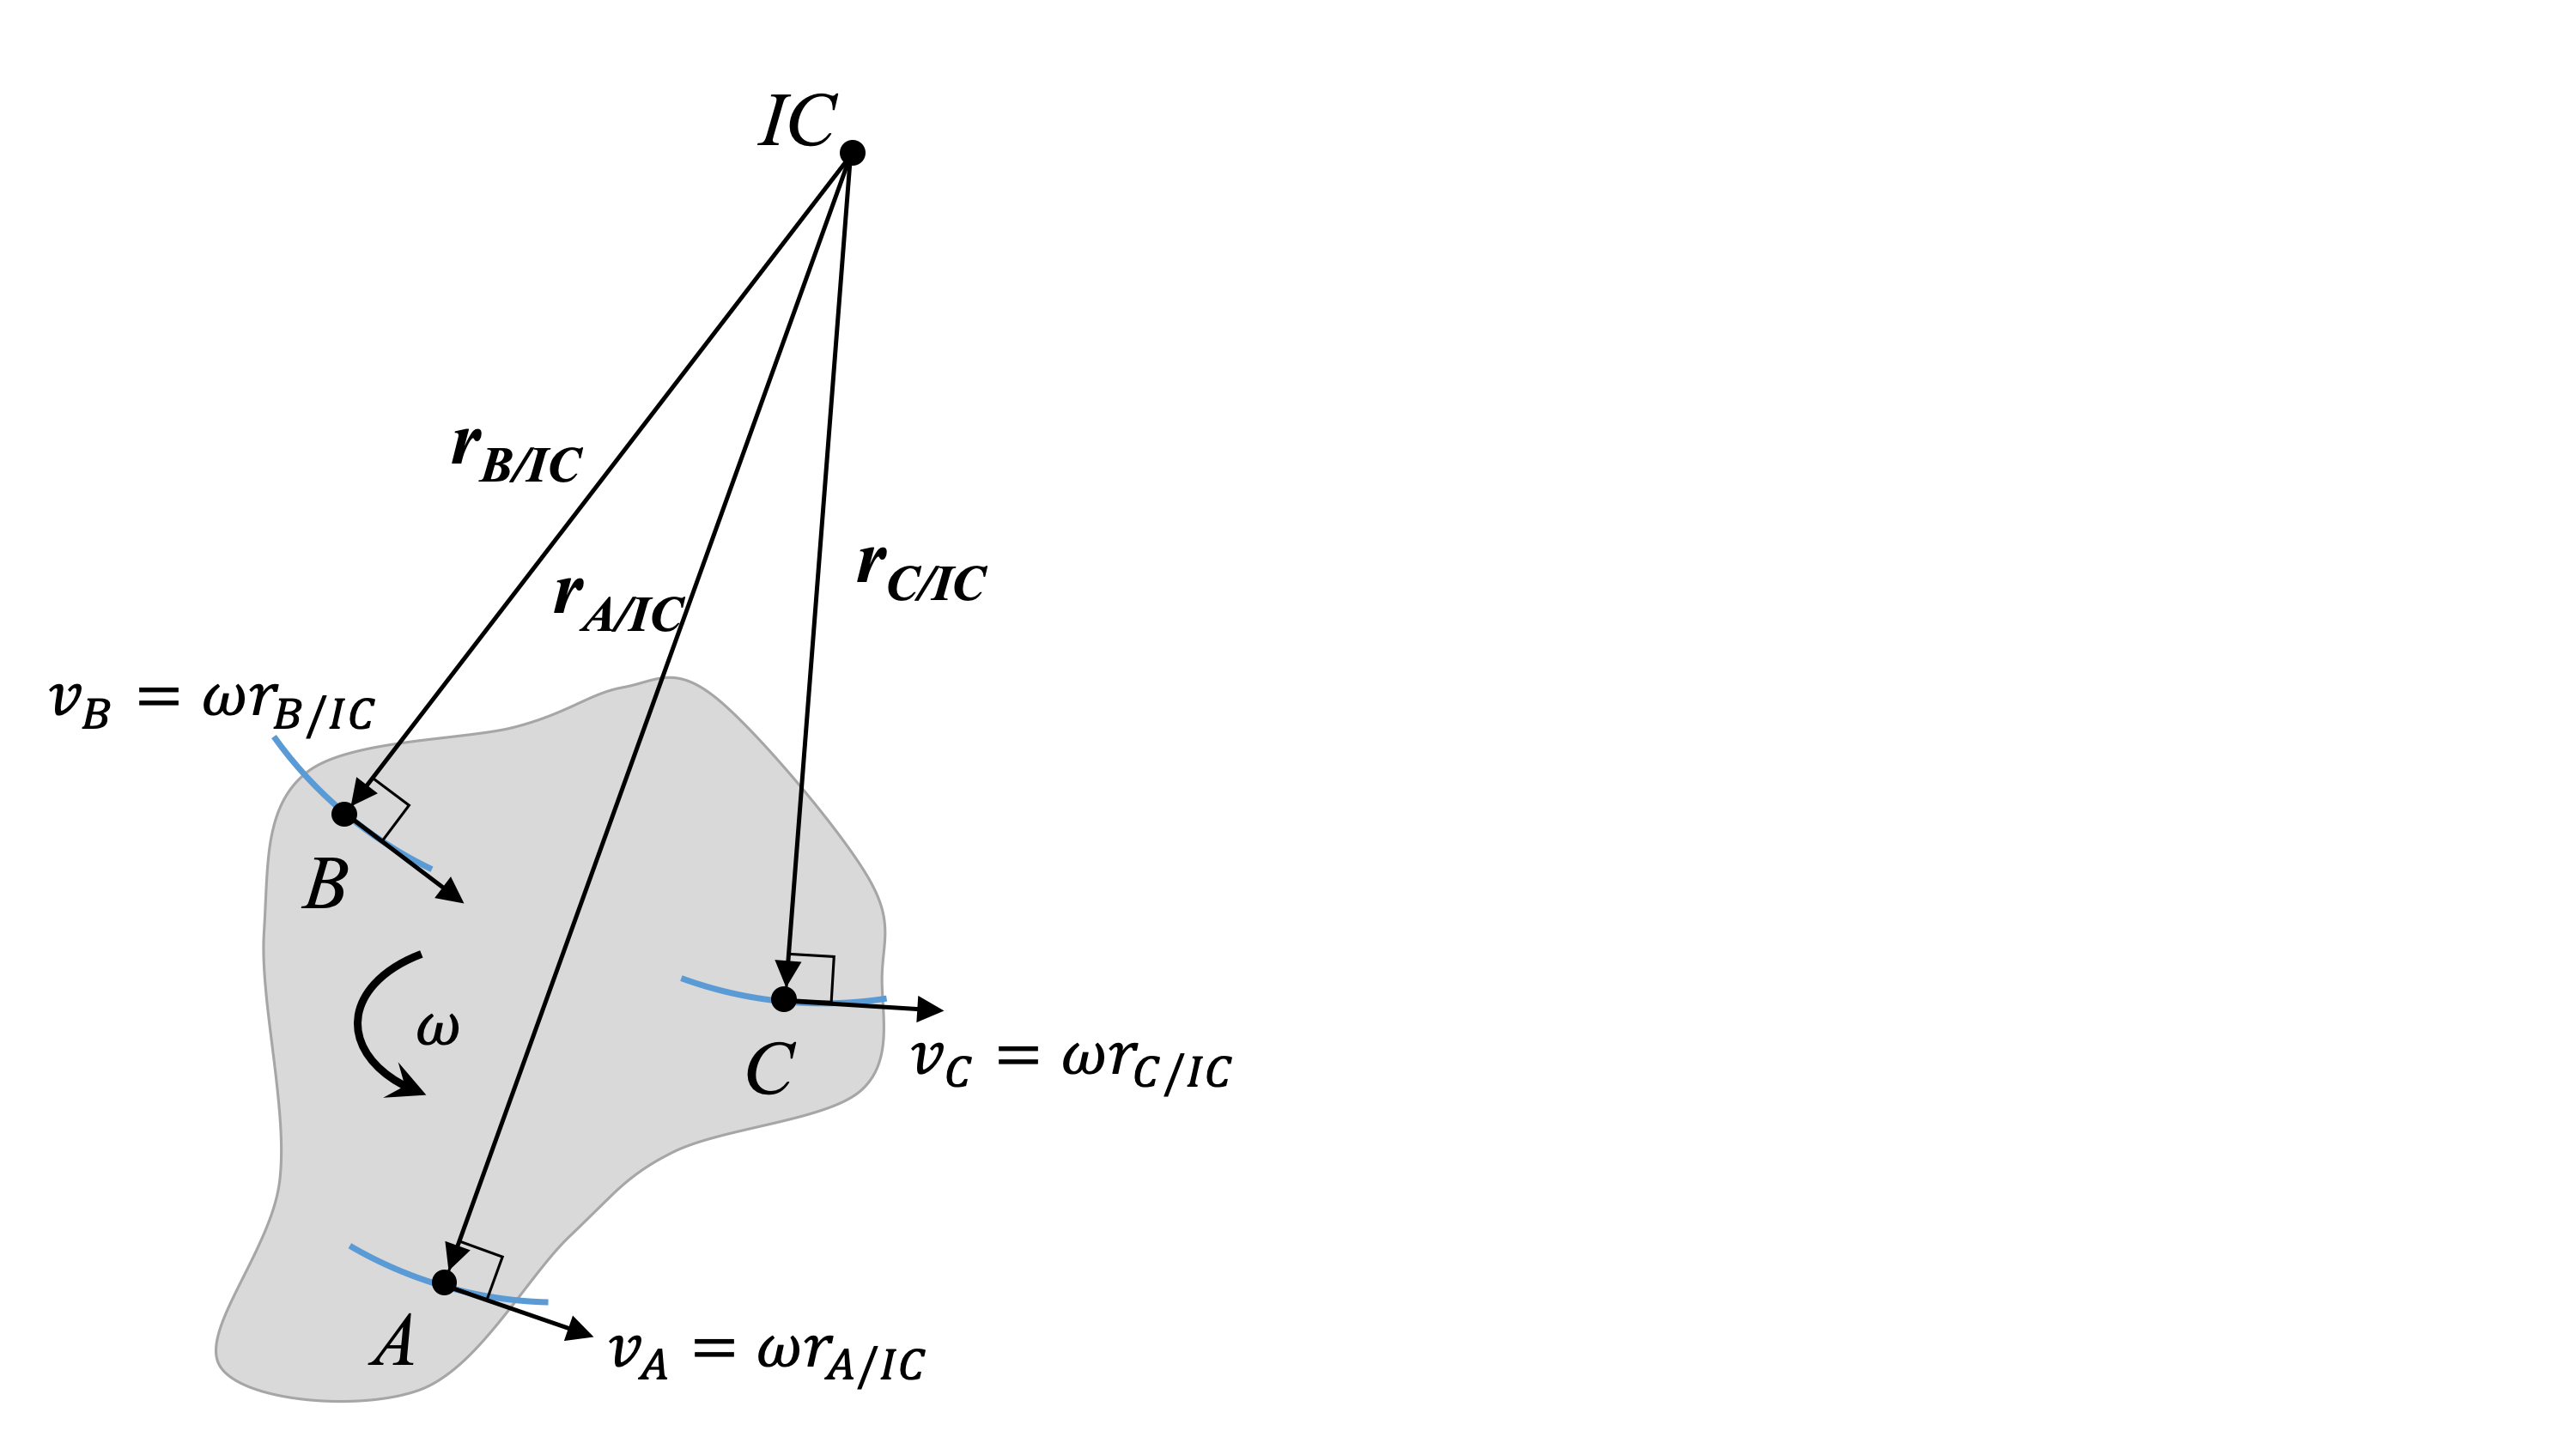
\includegraphics[trim={0cm 0cm 12cm 0cm},clip,width=0.5\textwidth, left]{Slide23} 

\vspace*{4\baselineskip}

\item If the velocities (magnitudes and directions) of two points on the rigid body are the same, then the body is NOT rotating, $\omega = 0$, $\bm{r_{IC}} = \infty$.

\newpage
\item If the velocities of two points on the rigid body are co-linear (along the same direction, but different magnitude and/or sense), the method for finding the ICZV differs.  There are three cases: 
\end{itemize}

\newpage
\subsection{Example 1}
Consider a yo-yo unraveling, without the string slipping.  Find $\bm{v_A}$ and $\bm{v_B}$ at the instant shown.  

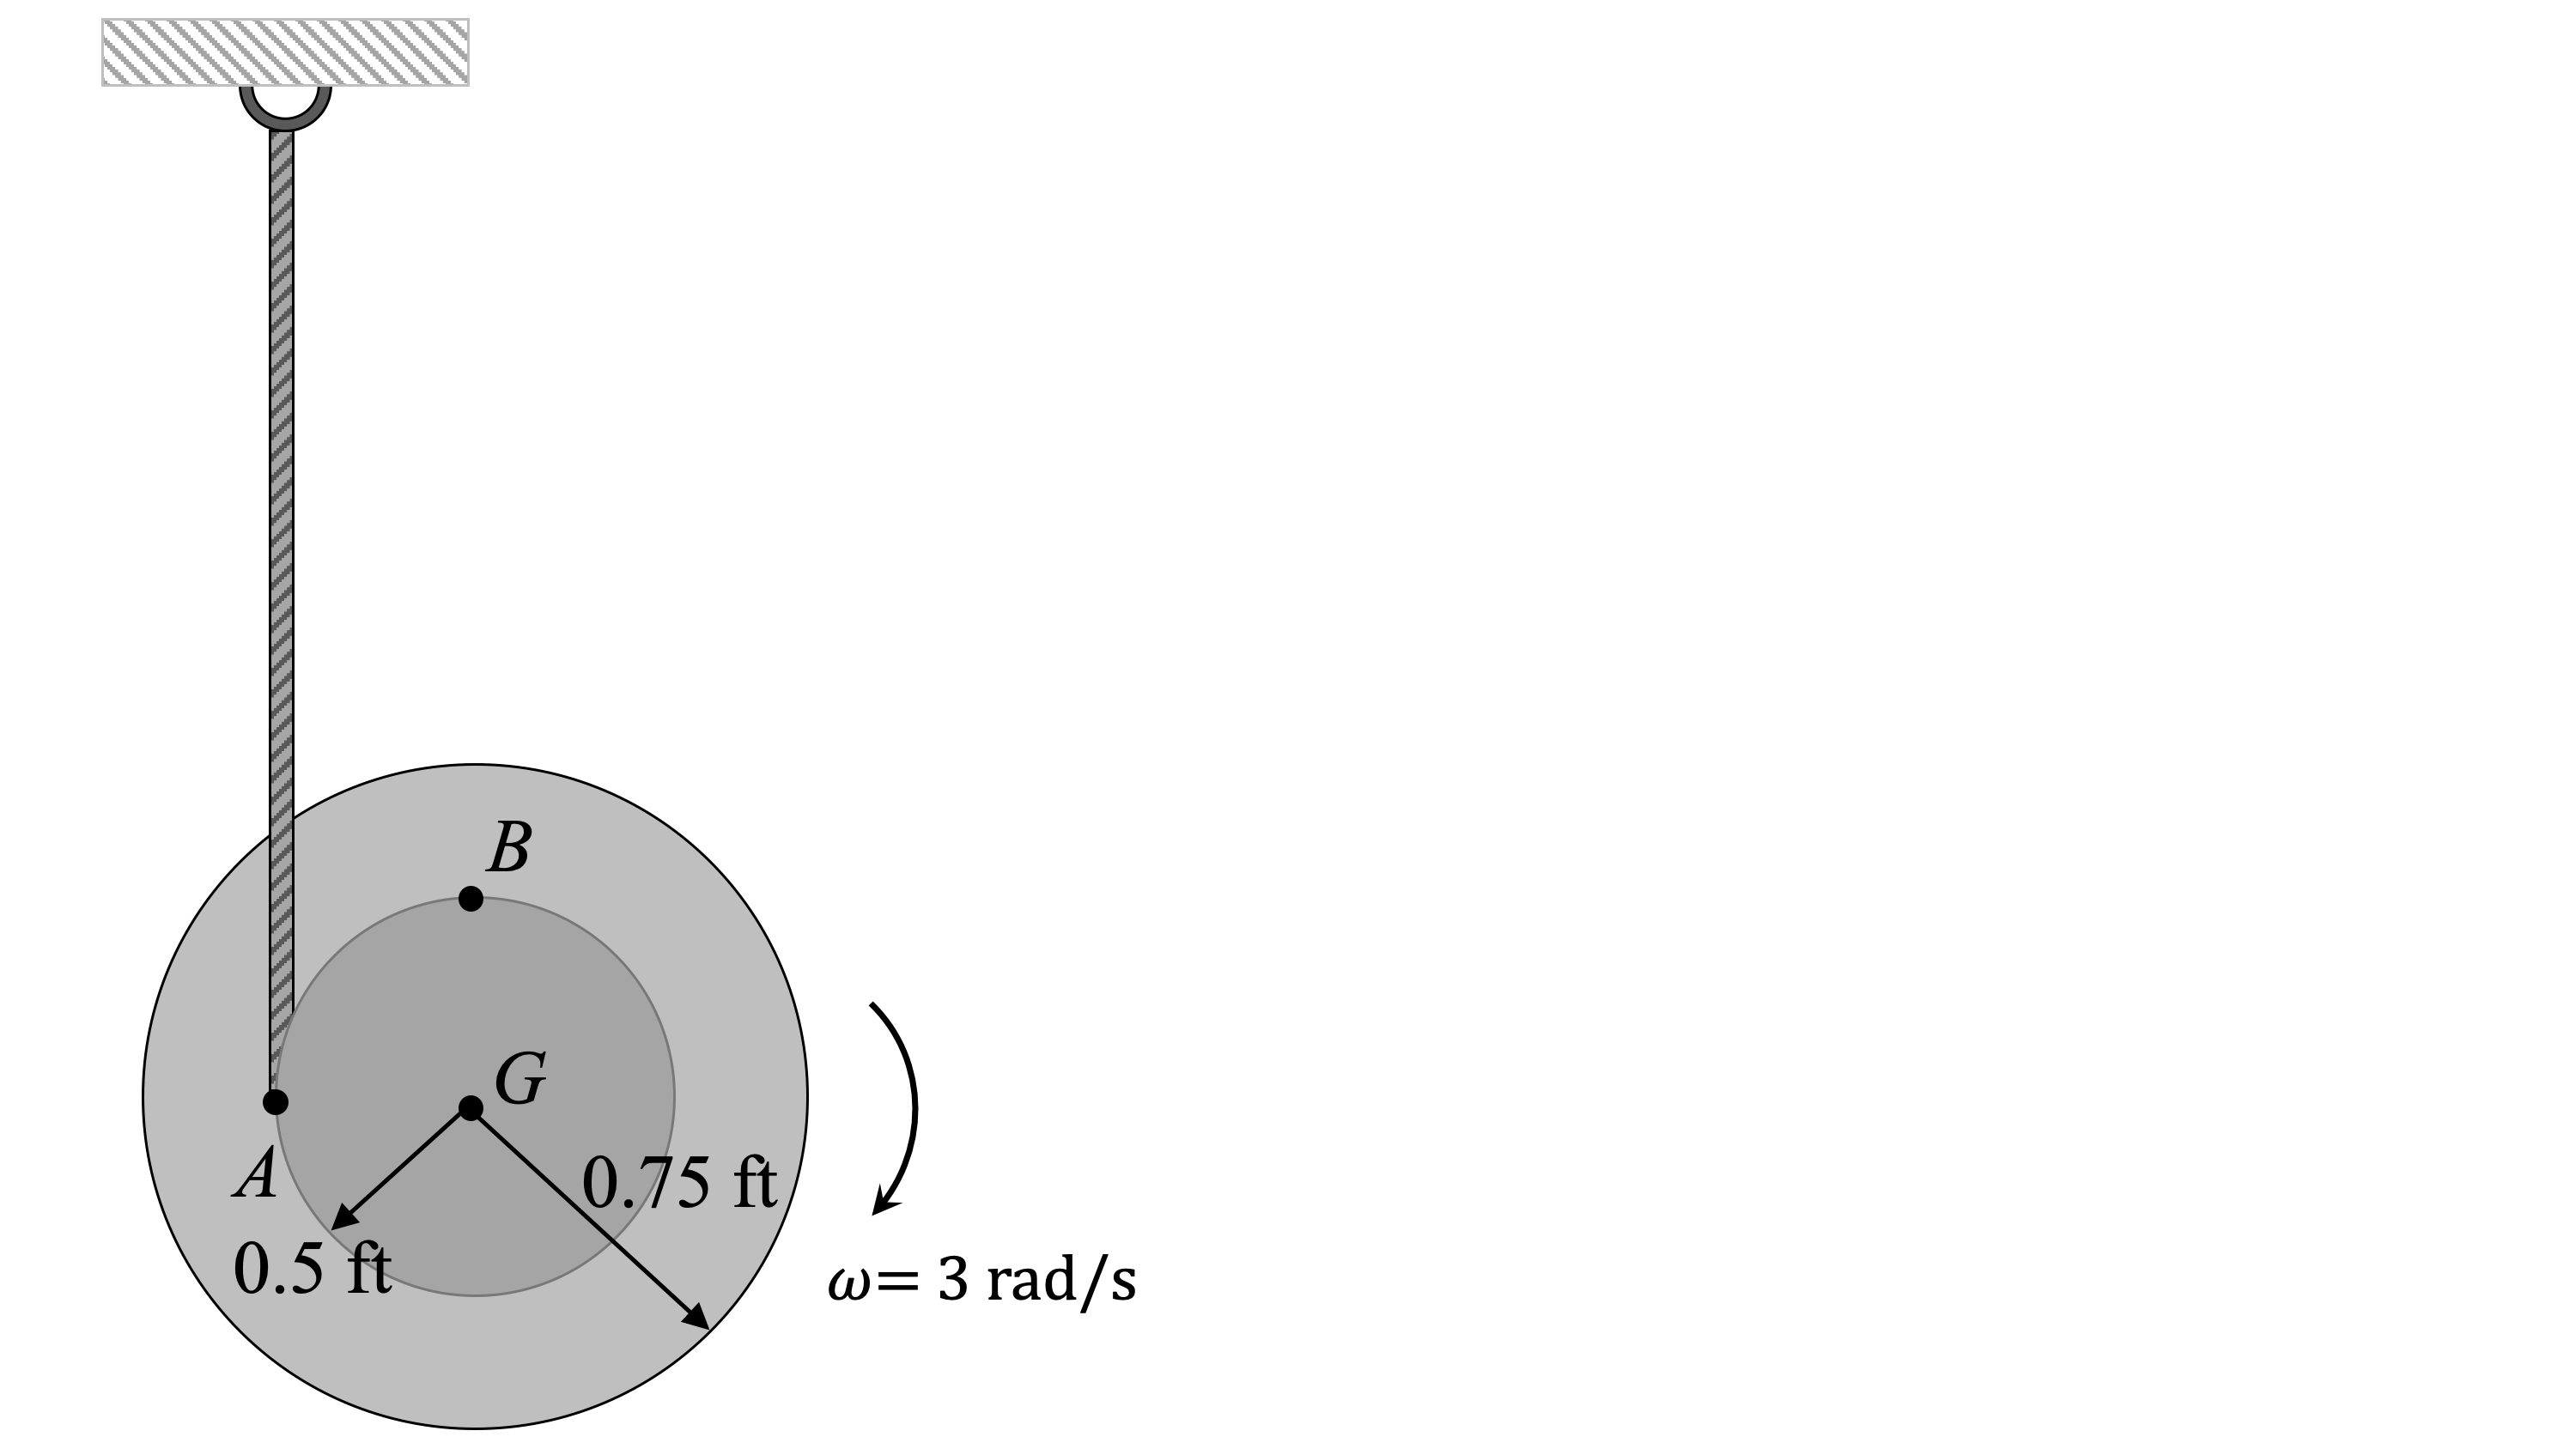
\includegraphics[trim={0cm 0cm 12cm 0cm},clip,width=0.45\textwidth, left]{Slide24} 
\newpage

\subsection{Example 2}
Consider the mechanism shown. Find the ICZV of bar $BC$ and the angular velocity of bar $CD$, $\bm{\omega_{CD}}$ at the instant shown, given $\bm{\omega_{AB}} = -1 \, rad/s \,  \bm{\hat{k}}$. 

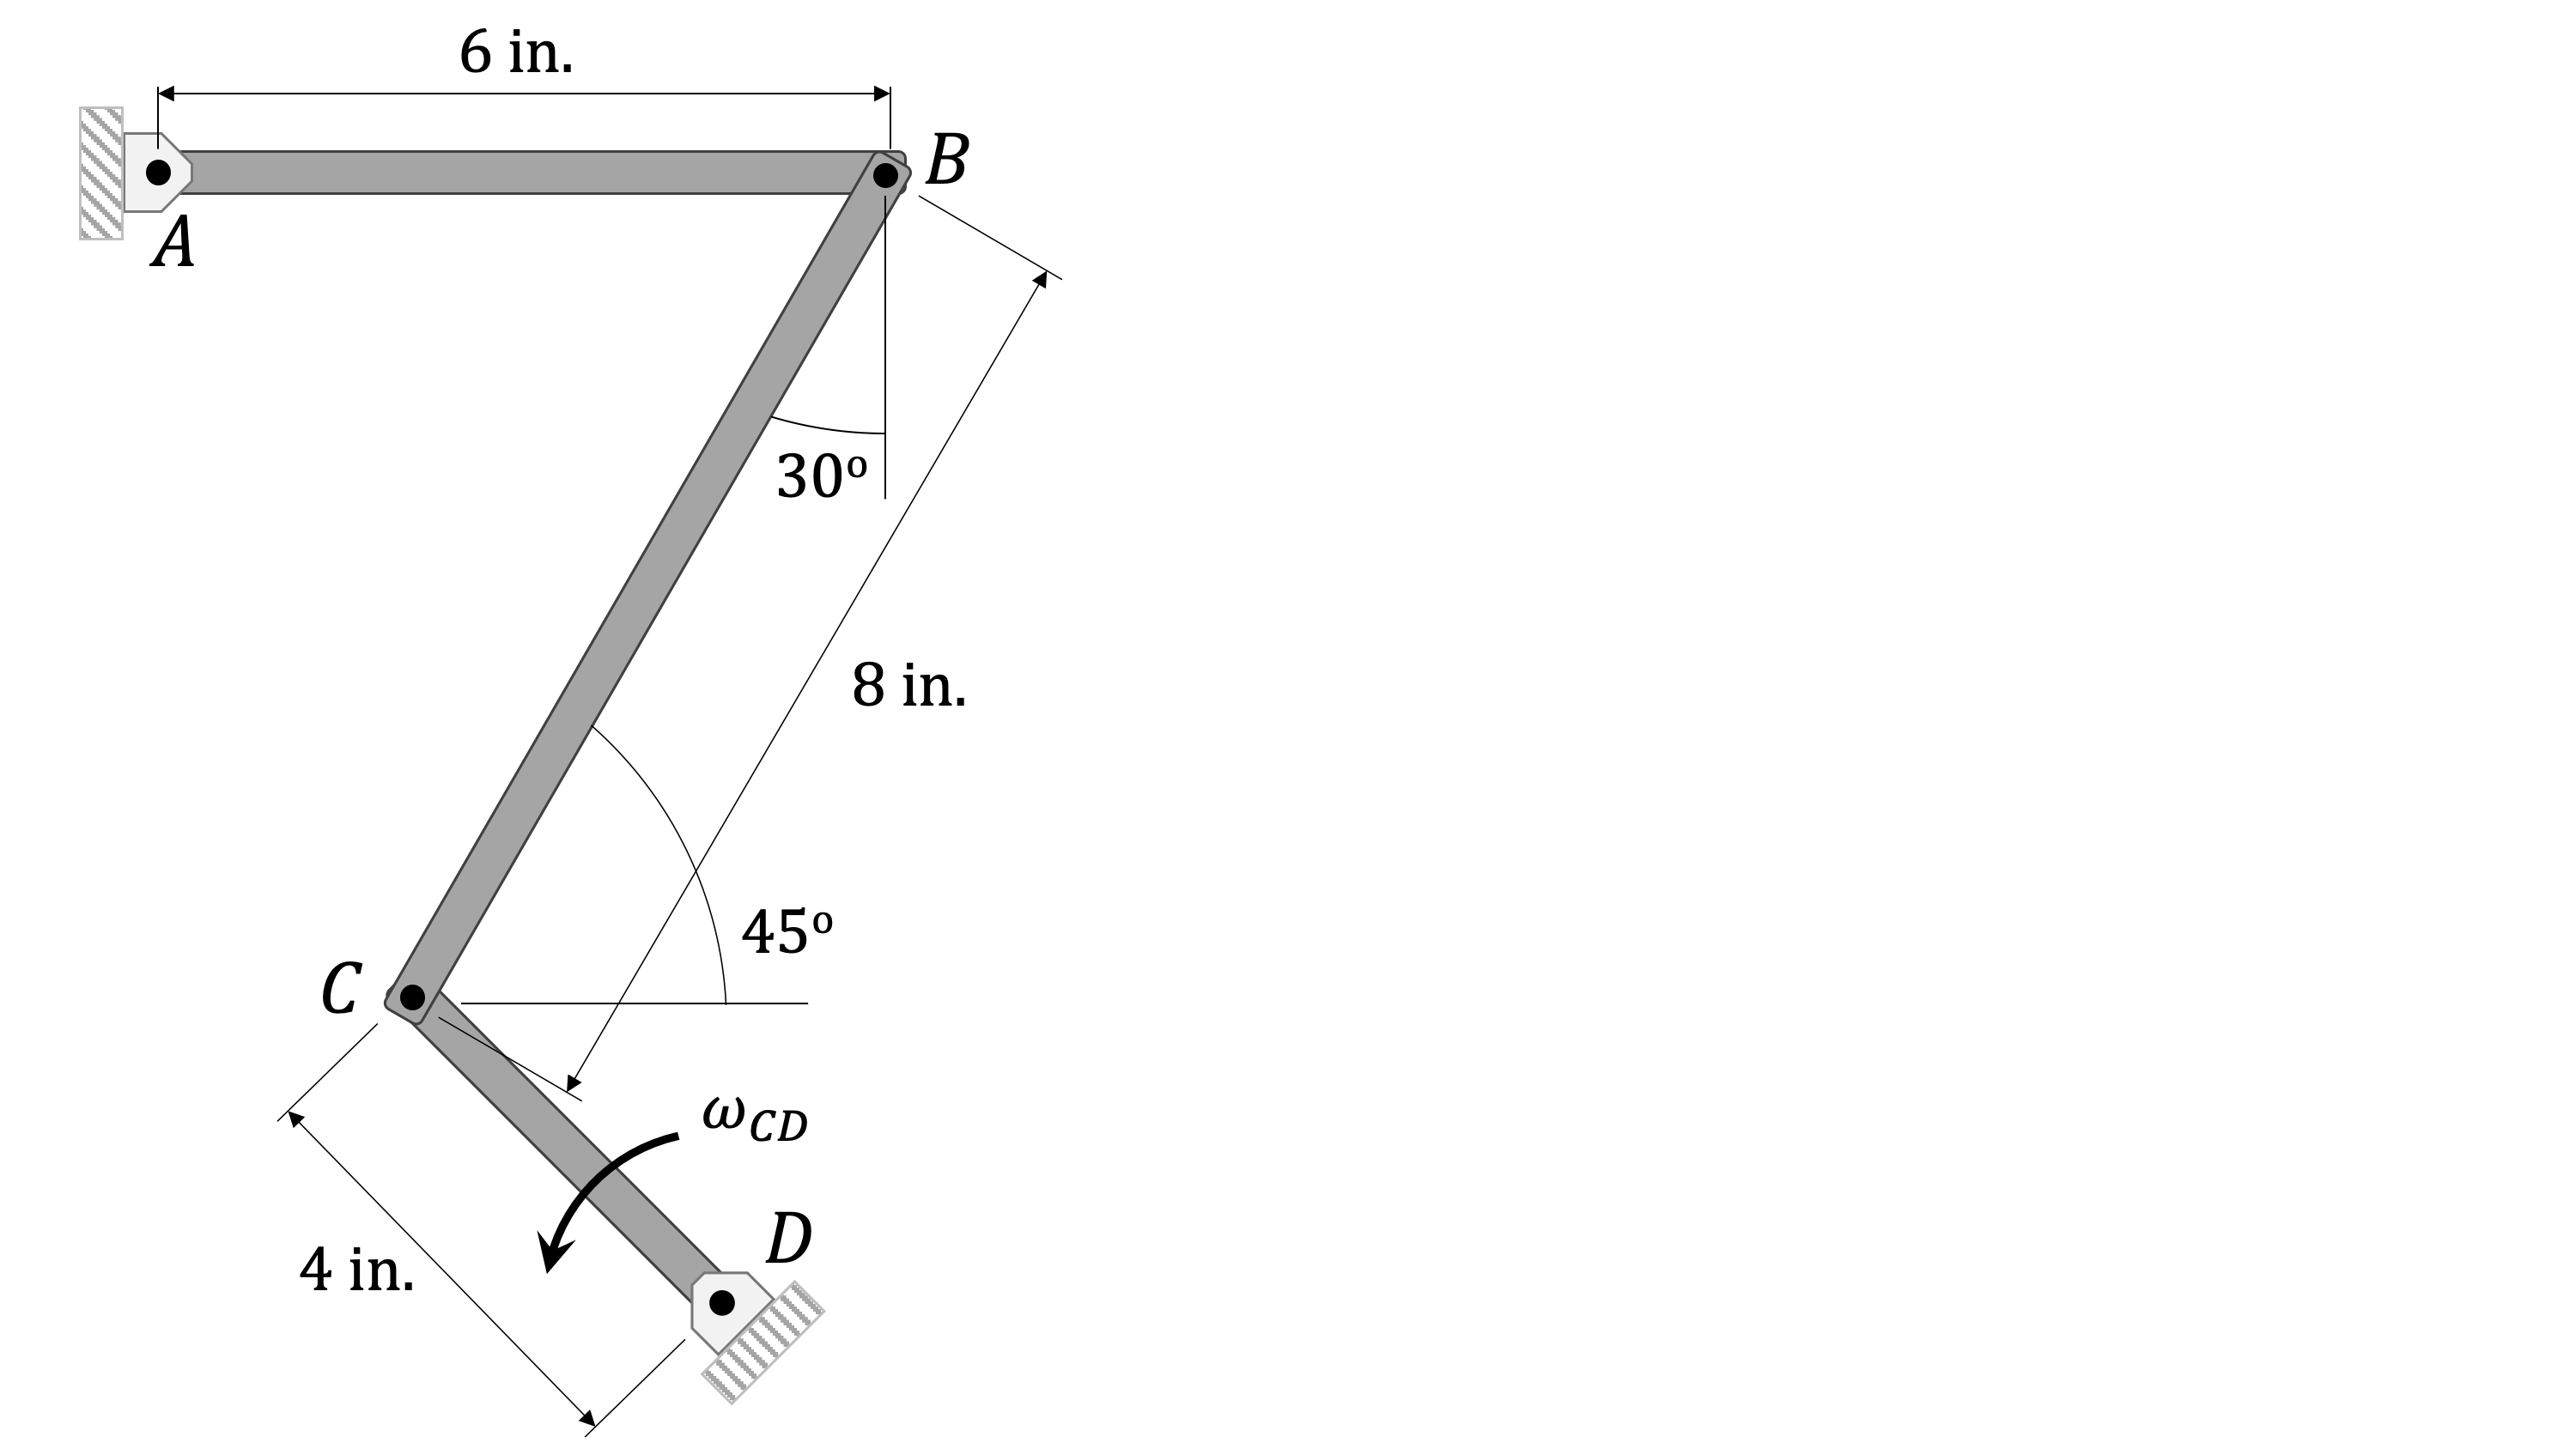
\includegraphics[trim={0cm 0cm 12cm 0cm},clip,width=0.55\textwidth, left]{Slide25} 
\newpage
(Example continued)

\chapter{L4: Relative Plane Motion, Acceleration - Fixed Frame}
Readings

\section{Objective}
To describe the planar acceleration of \textbf{any point} on a rigid body that is both translating and rotating.  

\section{Reference Frame - Translating, but NOT Rotating}
We have already established the following relationships for fixed reference frame $O_{xyz}$ and translating reference frame $A_{x'y'z'}$.  


\begin{minipage}[c]{0.3\textwidth}
\begin{tabular}{  c  }
Position:  \\
  \\
$\bm{r_B} = \bm{r_A} +  \bm{r_{B/A}}$ \\
 \\
Velocity:  \\
 \\
$\bm{v_B} = \bm{v_A} + \bm{\omega} \times \bm{r_{B/A}}$ \\
\end{tabular}
\label{tab:singlebest}
\end{minipage}%%%
\begin{minipage}[c]{0.8\textwidth}
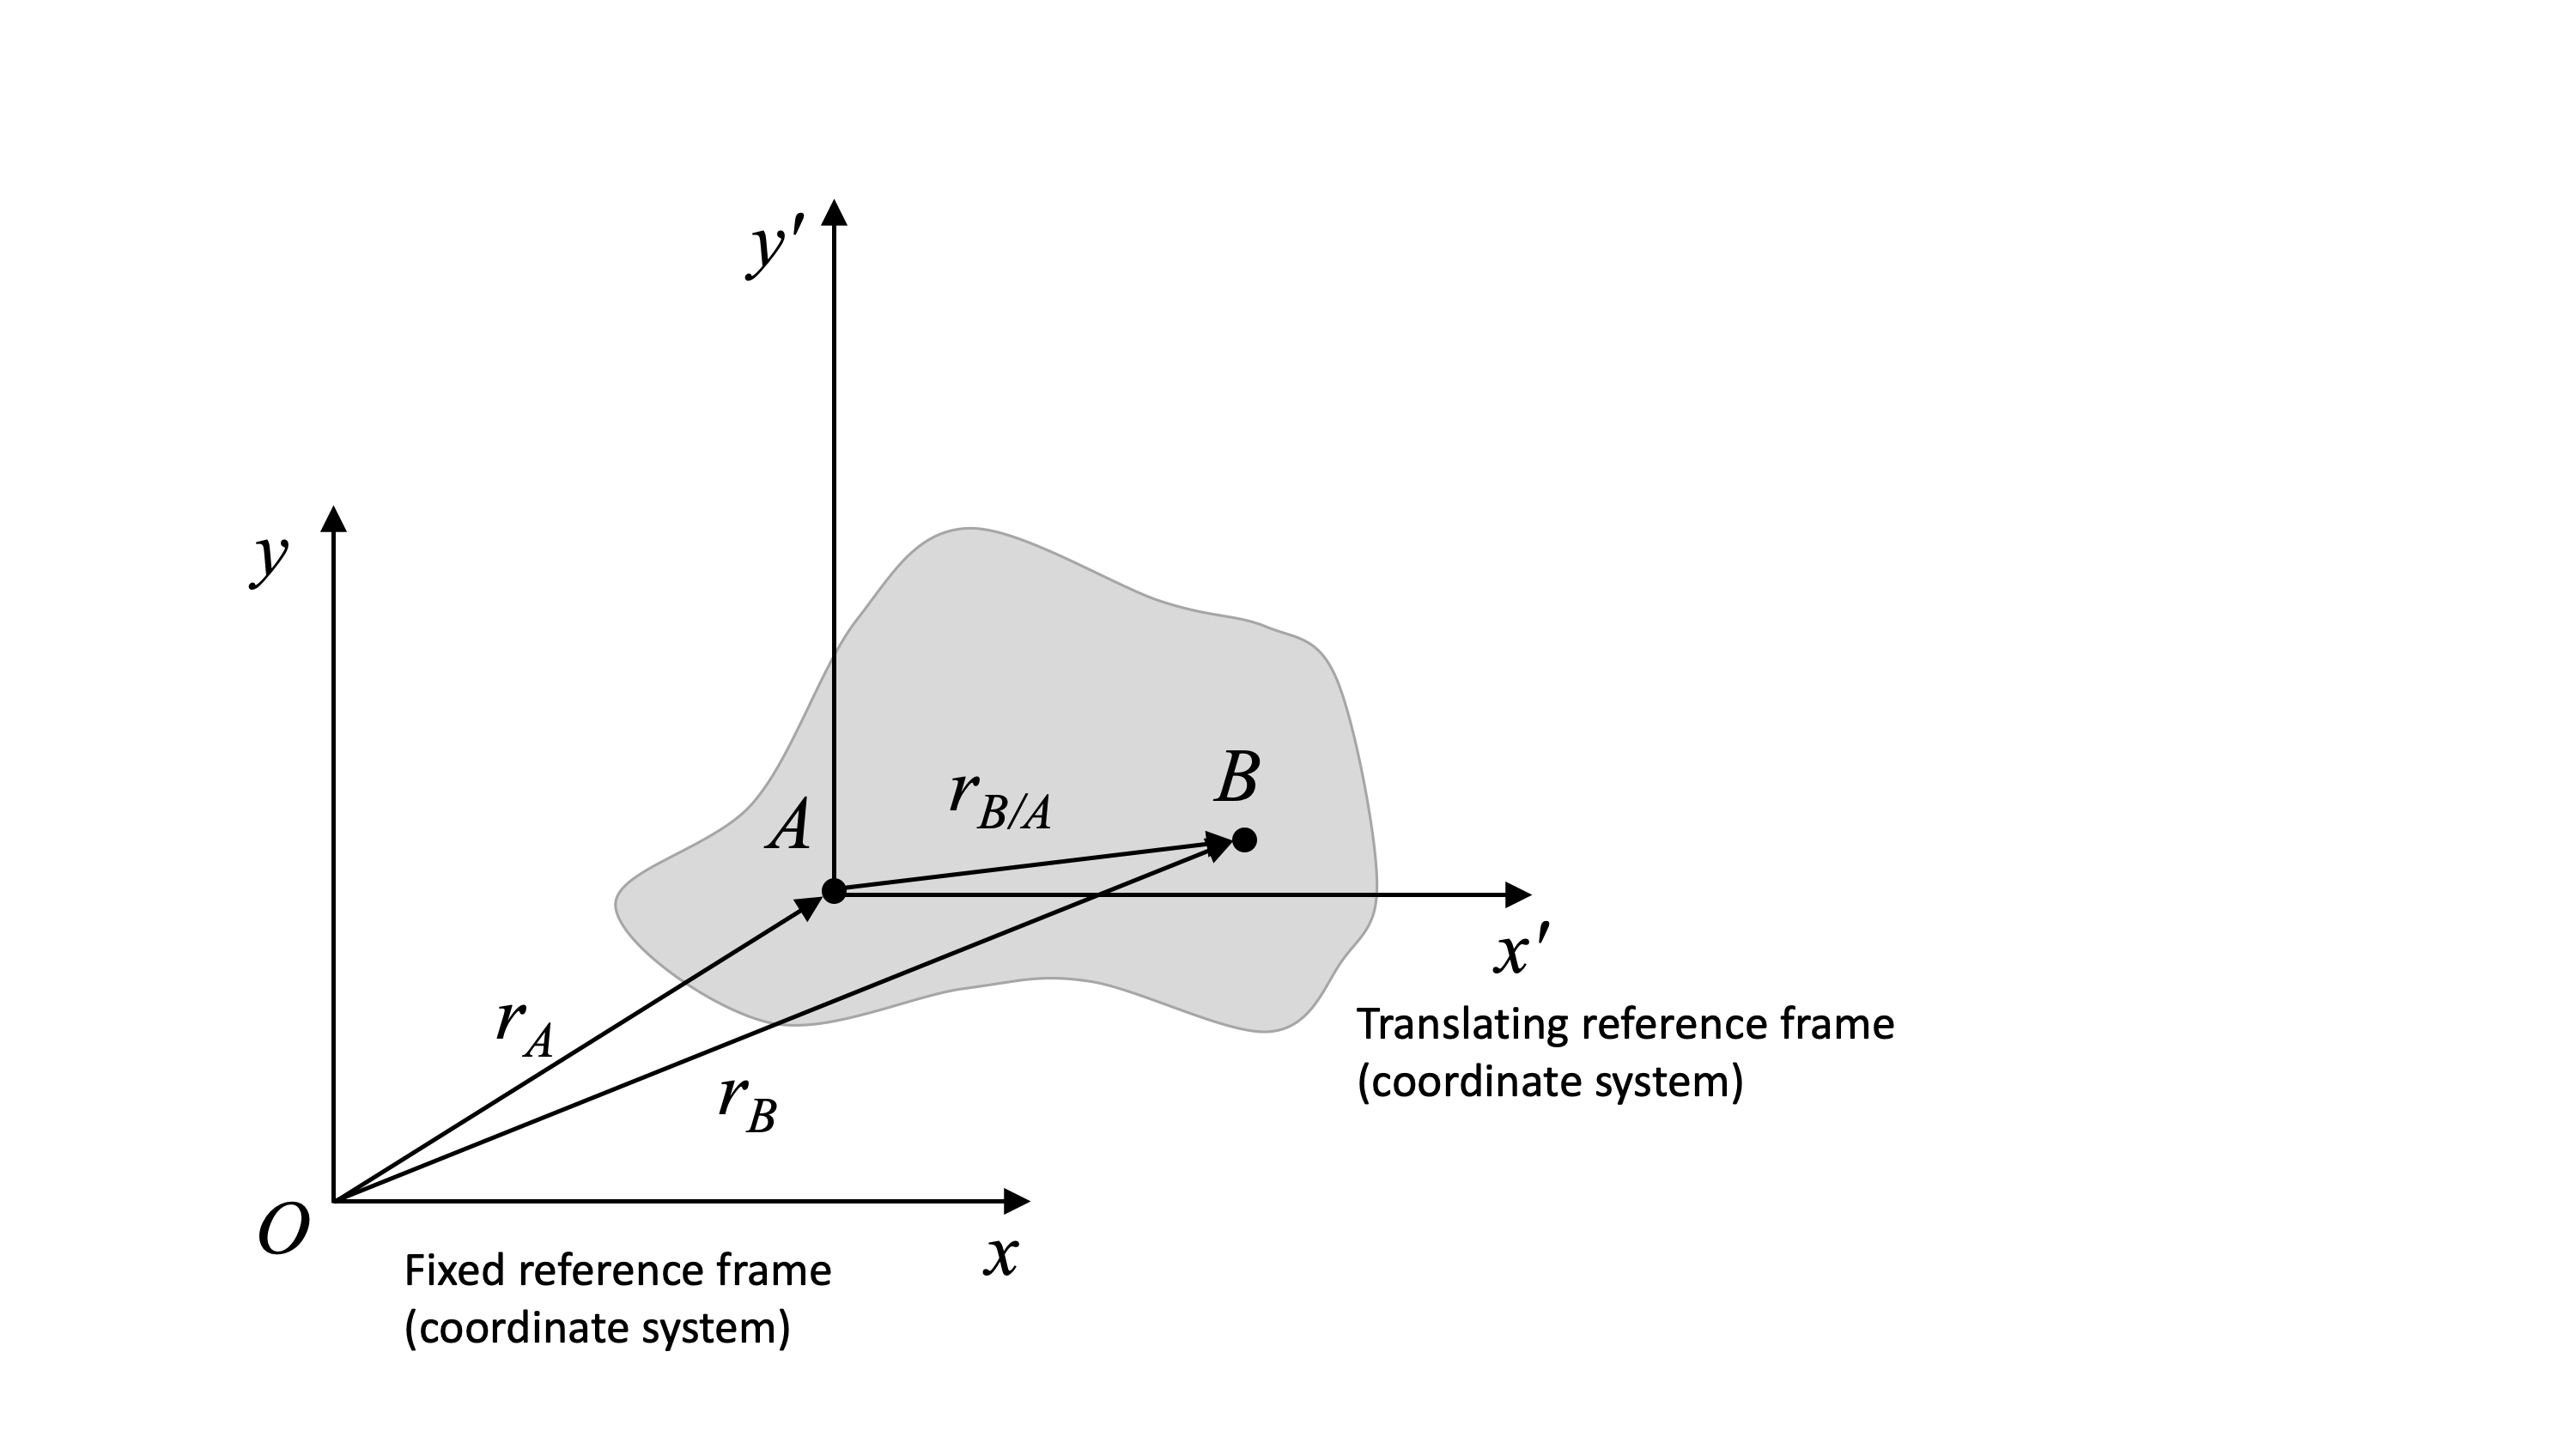
\includegraphics[trim={0cm 1cm 6cm 2cm},clip,width=1\textwidth, center]{Slide5} 
\end{minipage}

Once again, we need to differentiate to get acceleration:

\[
\bm{a_B} = \frac{d \bm{v_B}}{dt} = \frac{d \bm{v_A}}{dt} + \frac{d \omega \times \bm{r_{B/A}}}{dt} \]

\vspace*{2\baselineskip}
\[
\bm{a_B} = \bm{a_A} + \bm{\alpha} \times \bm{r_{B/A}} + \bm{\omega} \times (\bm{\omega} \times \bm{r_{B/A}})
\]

\vspace*{1\baselineskip}
\raggedbottom
\newpage

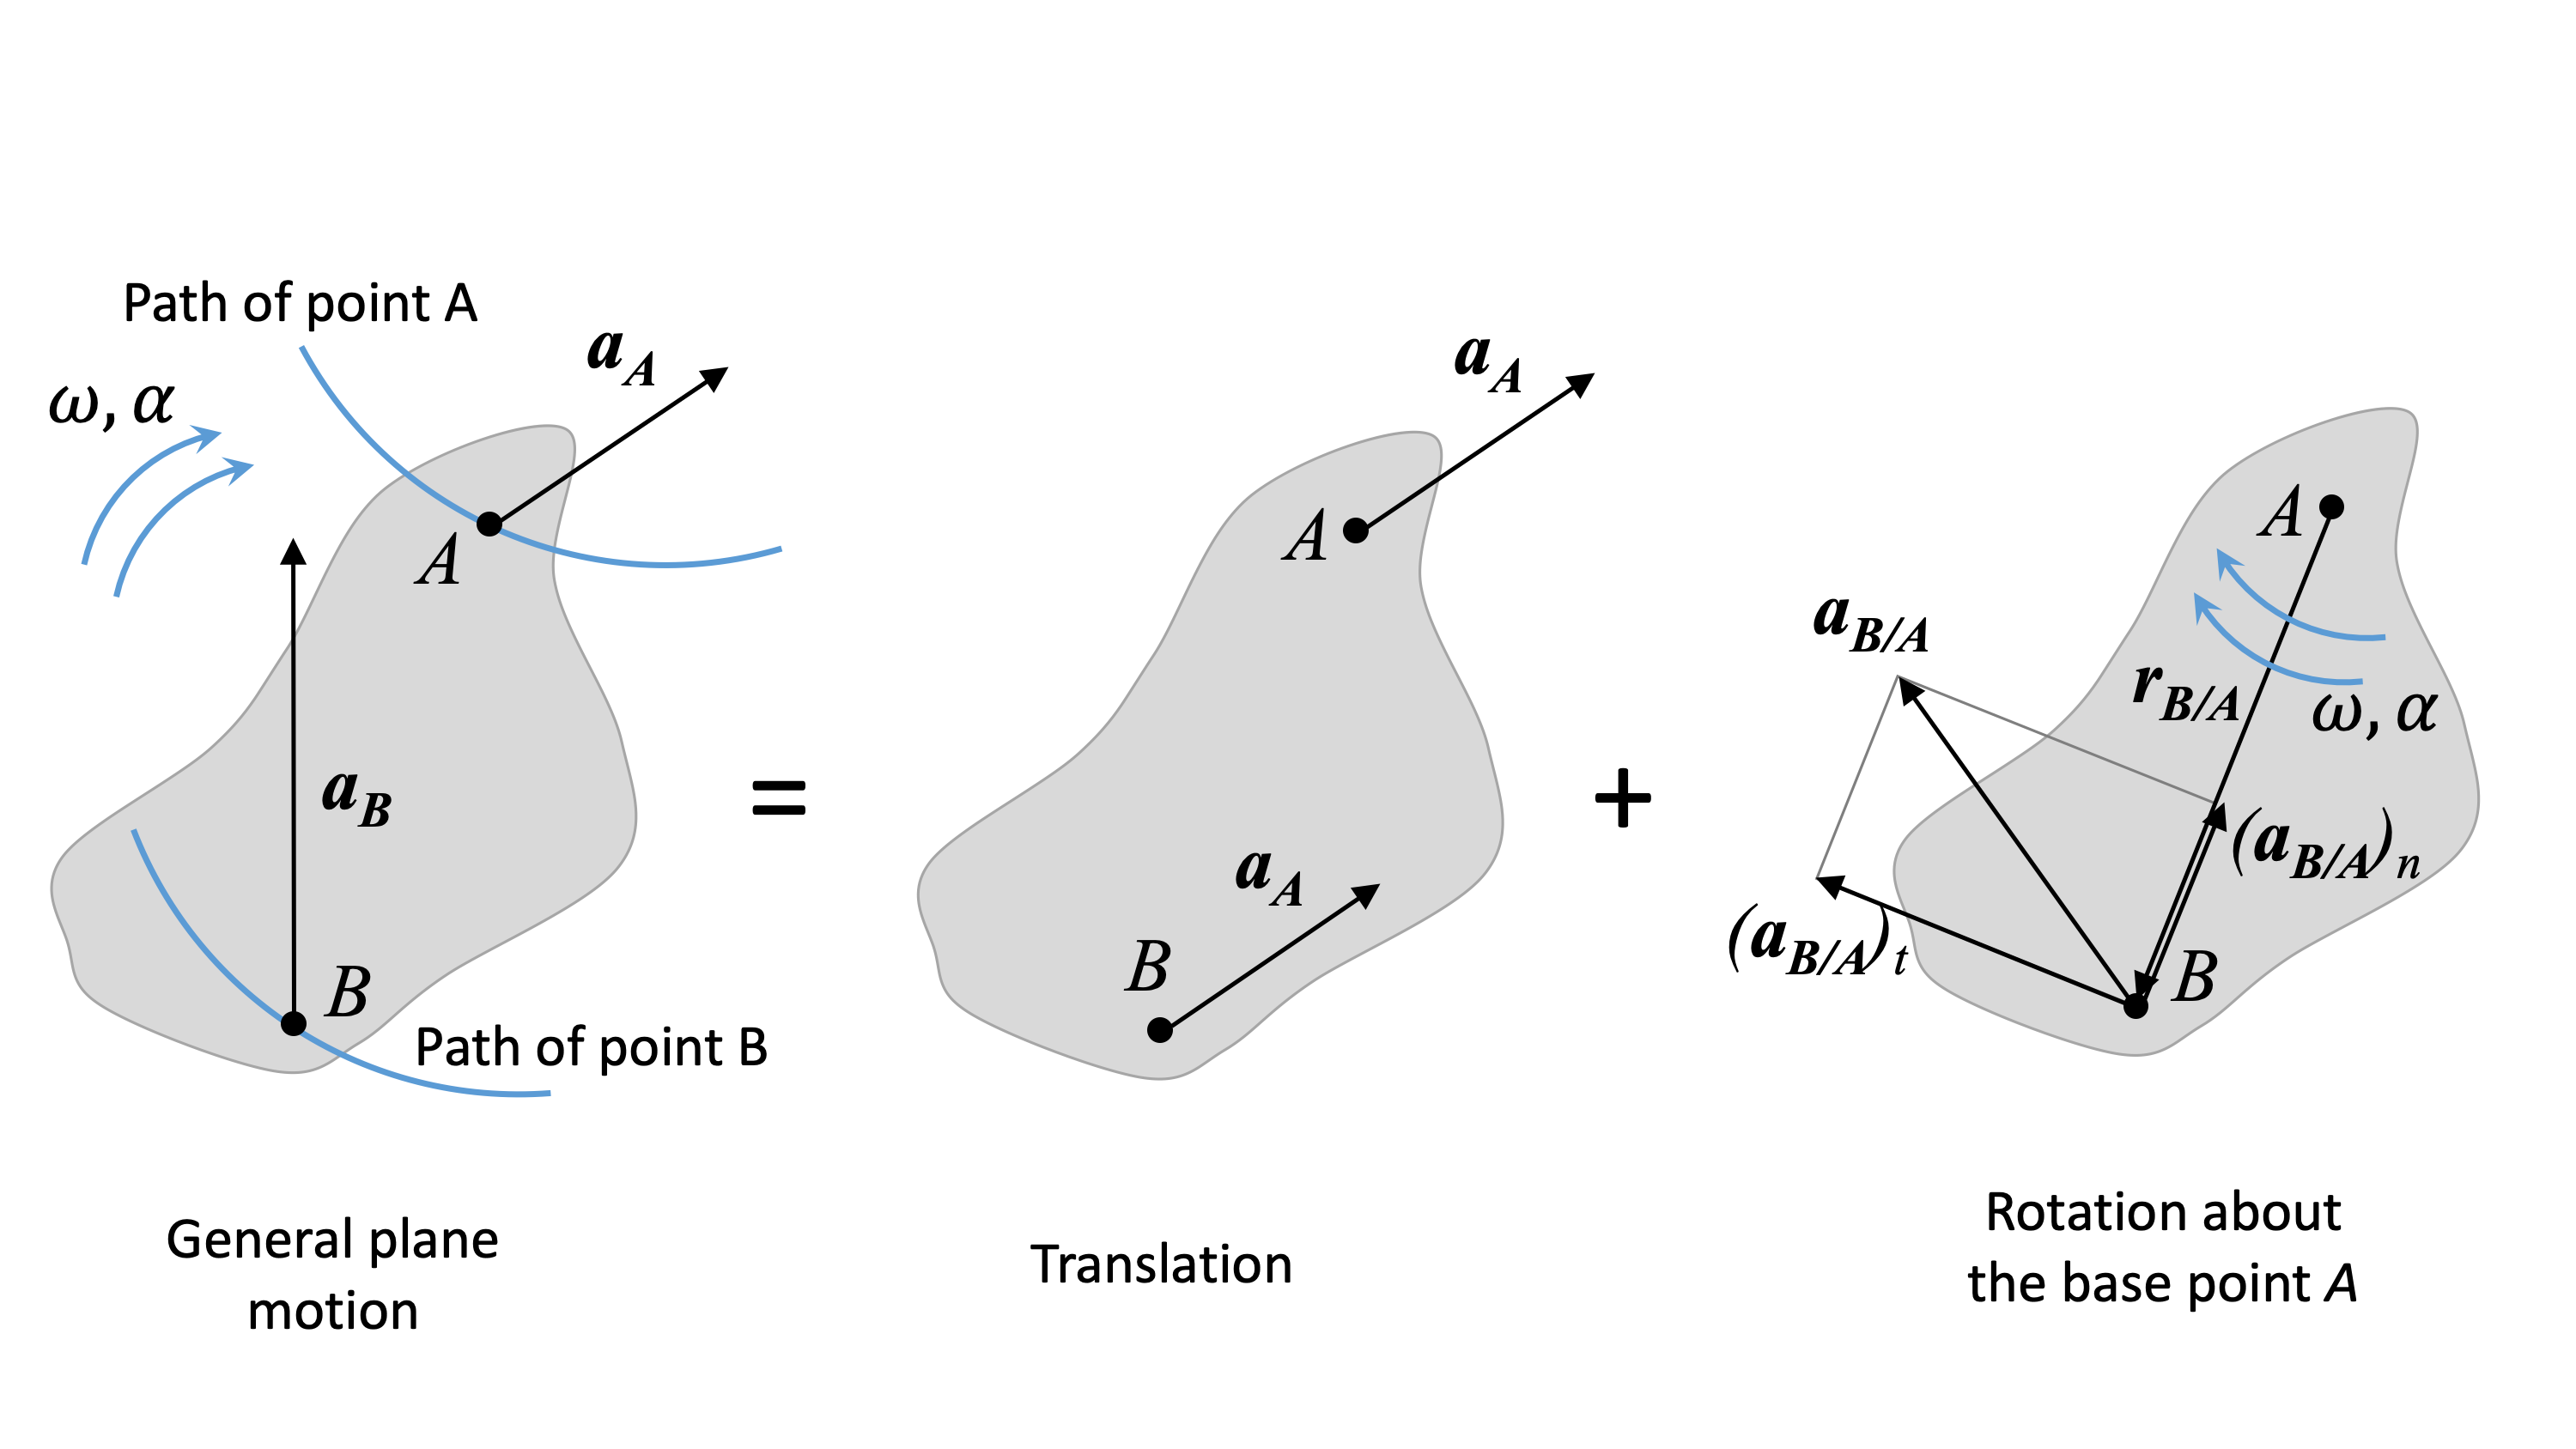
\includegraphics[trim={0cm 0.5cm 0cm 2.5cm},clip,width=1\textwidth, center]{Slide27} 

\vspace*{8\baselineskip}
What about that third term, $\bm{\omega} \times (\bm{\omega} \times \bm{r_{B/A}})$?
\vspace*{12\baselineskip}

Final result for acceleration with a translating reference frame:

\[ \bm{a_B} = \bm{a_A} + \bm{\alpha} \times \bm{r_{B/A}} - \omega^2   \bm{r_{B/A}}
\]
\vspace*{2\baselineskip}

\subsection{Example 1}
Consider a wheel rolling without slipping.  Find the velocity and acceleration of point $G$ in the $xyz$ frame shown.  Also, find the velocity and acceleration of a point $B$ at the front of the wheel.  $r = 1 \, m$, $\bm{\omega} = -1 \, rad/s \, \bm{\hat{k}}$, $\bm{\alpha} = 1 \, rad/s^2 \, \bm{\hat{k}}$. 

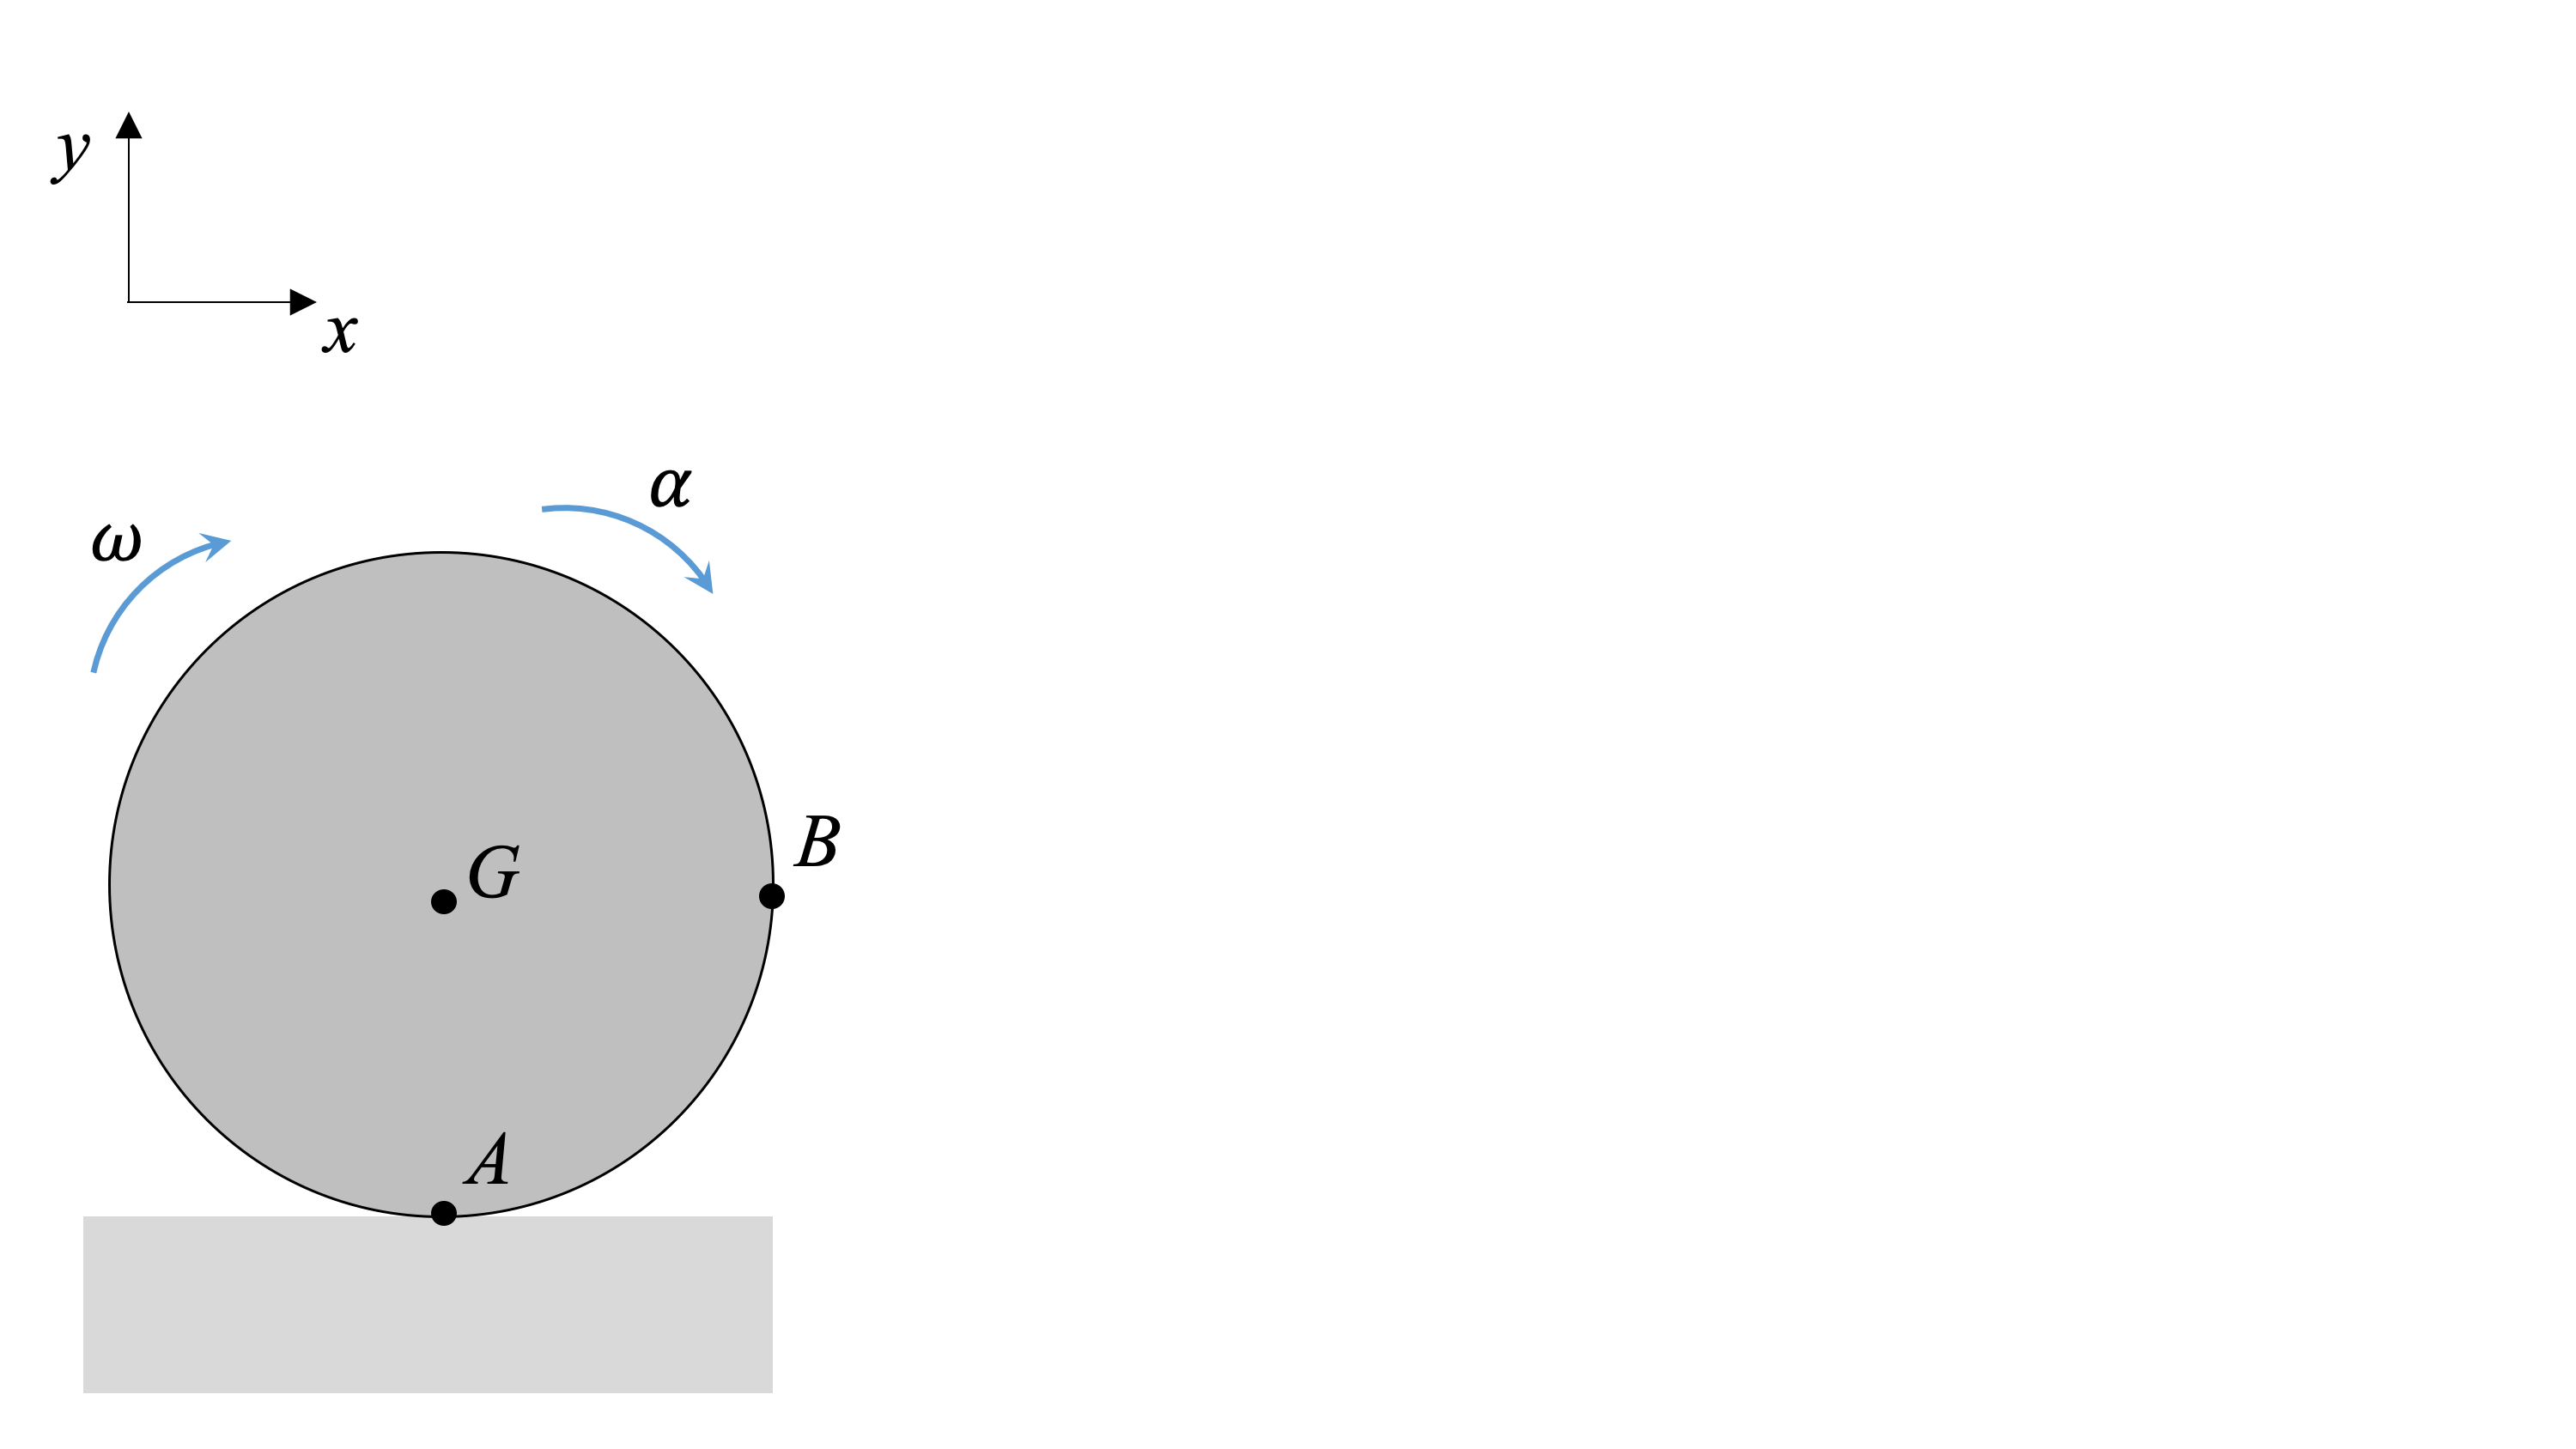
\includegraphics[trim={0cm 0cm 15cm 0cm},clip,width=0.4\textwidth, left]{Slide28} 

\newpage
(Example continued)

\vspace*{22\baselineskip}
\newpage

\subsection{Example 2}
Consider a planar robot pushing a grinding wheel over a surface (robotic de-burring). Find the angular velocity and acceleration of each link (at the instant shown) necessary to keep the grinding wheel moving to the right at a constant $1 \, m/s$.

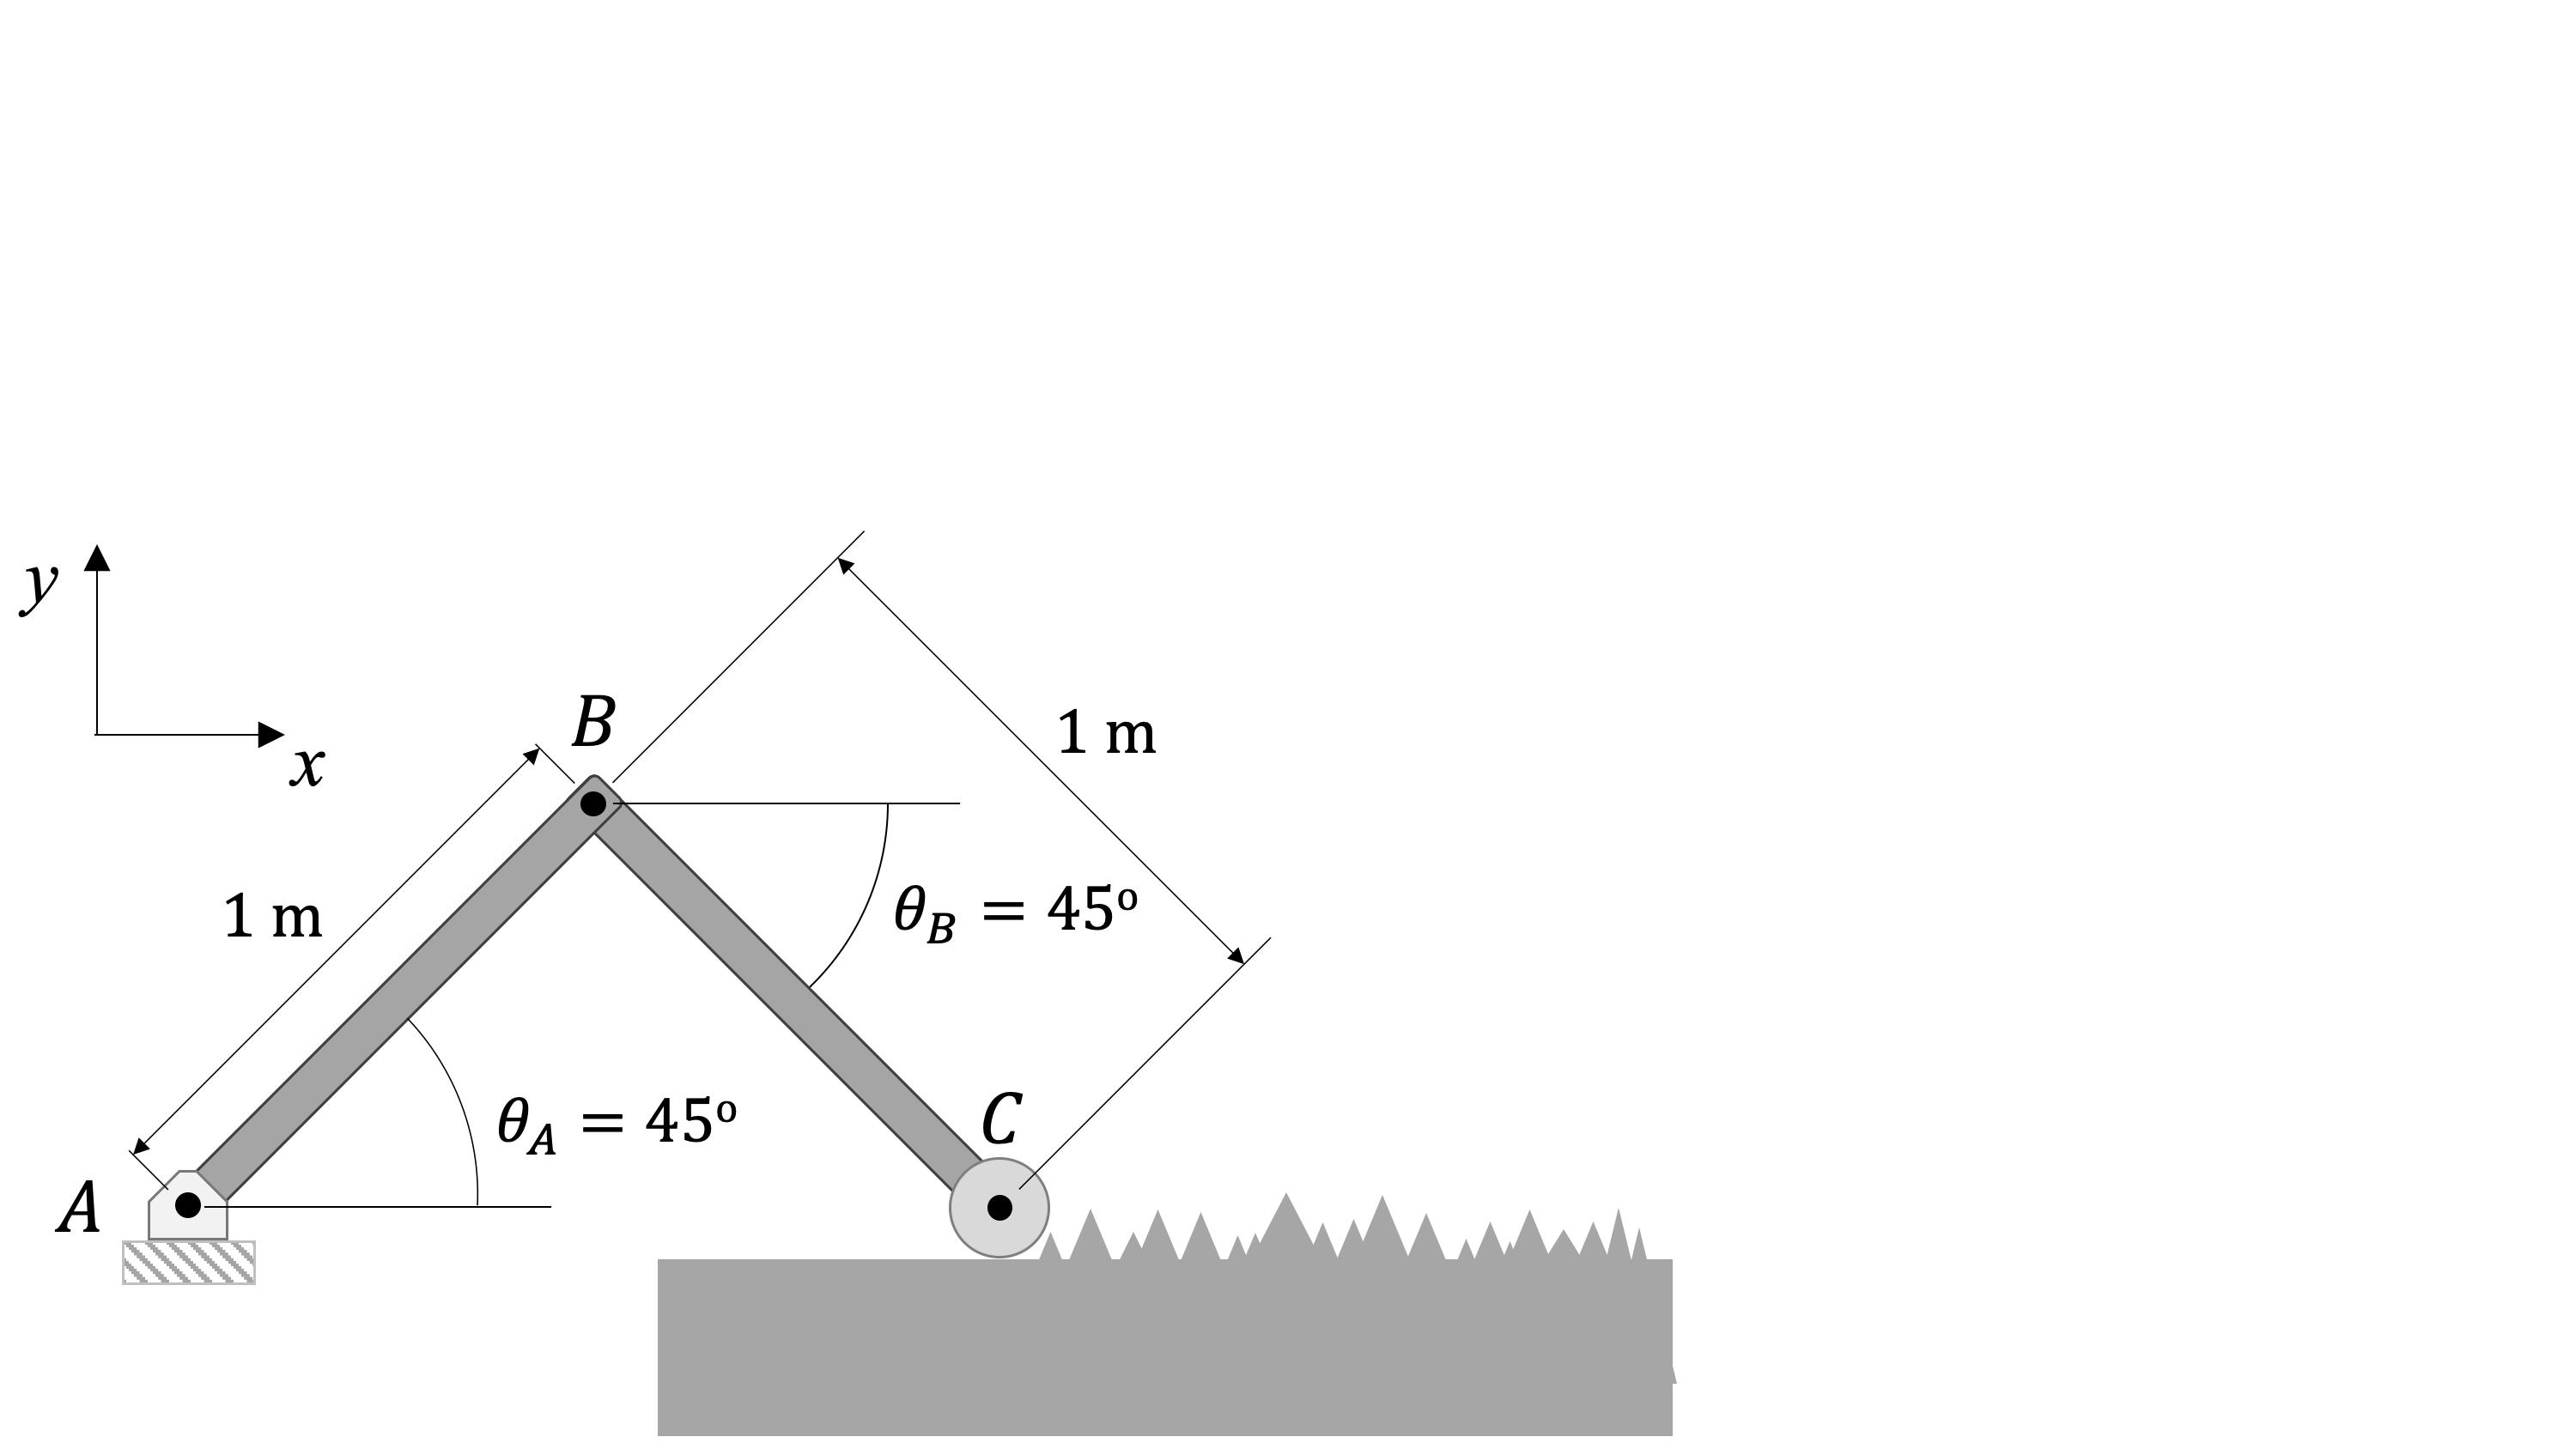
\includegraphics[trim={0cm 0cm 12cm 7cm},clip,width=0.6\textwidth, left]{Slide29} 

\newpage
(Example continued)

\chapter{L5/L6: Relative Plane Motion - Rotating Frame}
Readings

\section{Objective}
To describe the planar velocity and acceleration of one rigid body which is moving with general plane motion with respect to another moving body.  For example, the body is:
\begin{itemize}
\item Sliding with respect to another moving body.
\item Moving with general plane motion with respect to another moving body. 
\end{itemize}

\section{Reference Frames}
Up until now, we have dealt with two frames: fixed reference frame $O_{xyz}$ and translating reference frame $A_{x'y'z'}$. 

\begin{minipage}[c]{0.4\textwidth}
\begin{tabular}{  c  }
Position:  \\
  \\
$\bm{r_B} = \bm{r_A} +  \bm{r_{B/A}}$ \\
 \\
Velocity:  \\
 \\
$\bm{v_B} = \bm{v_A} + \bm{\omega} \times \bm{r_{B/A}}$ \\
\\
Acceleration: \\
$\bm{a_B} = \bm{a_A} + \bm{\alpha} \times \bm{r_{B/A}} - \omega^2   \bm{r_{B/A}}$\\
\end{tabular}
\label{tab:singlebest}
\end{minipage}%%%
\begin{minipage}[c]{0.65\textwidth}
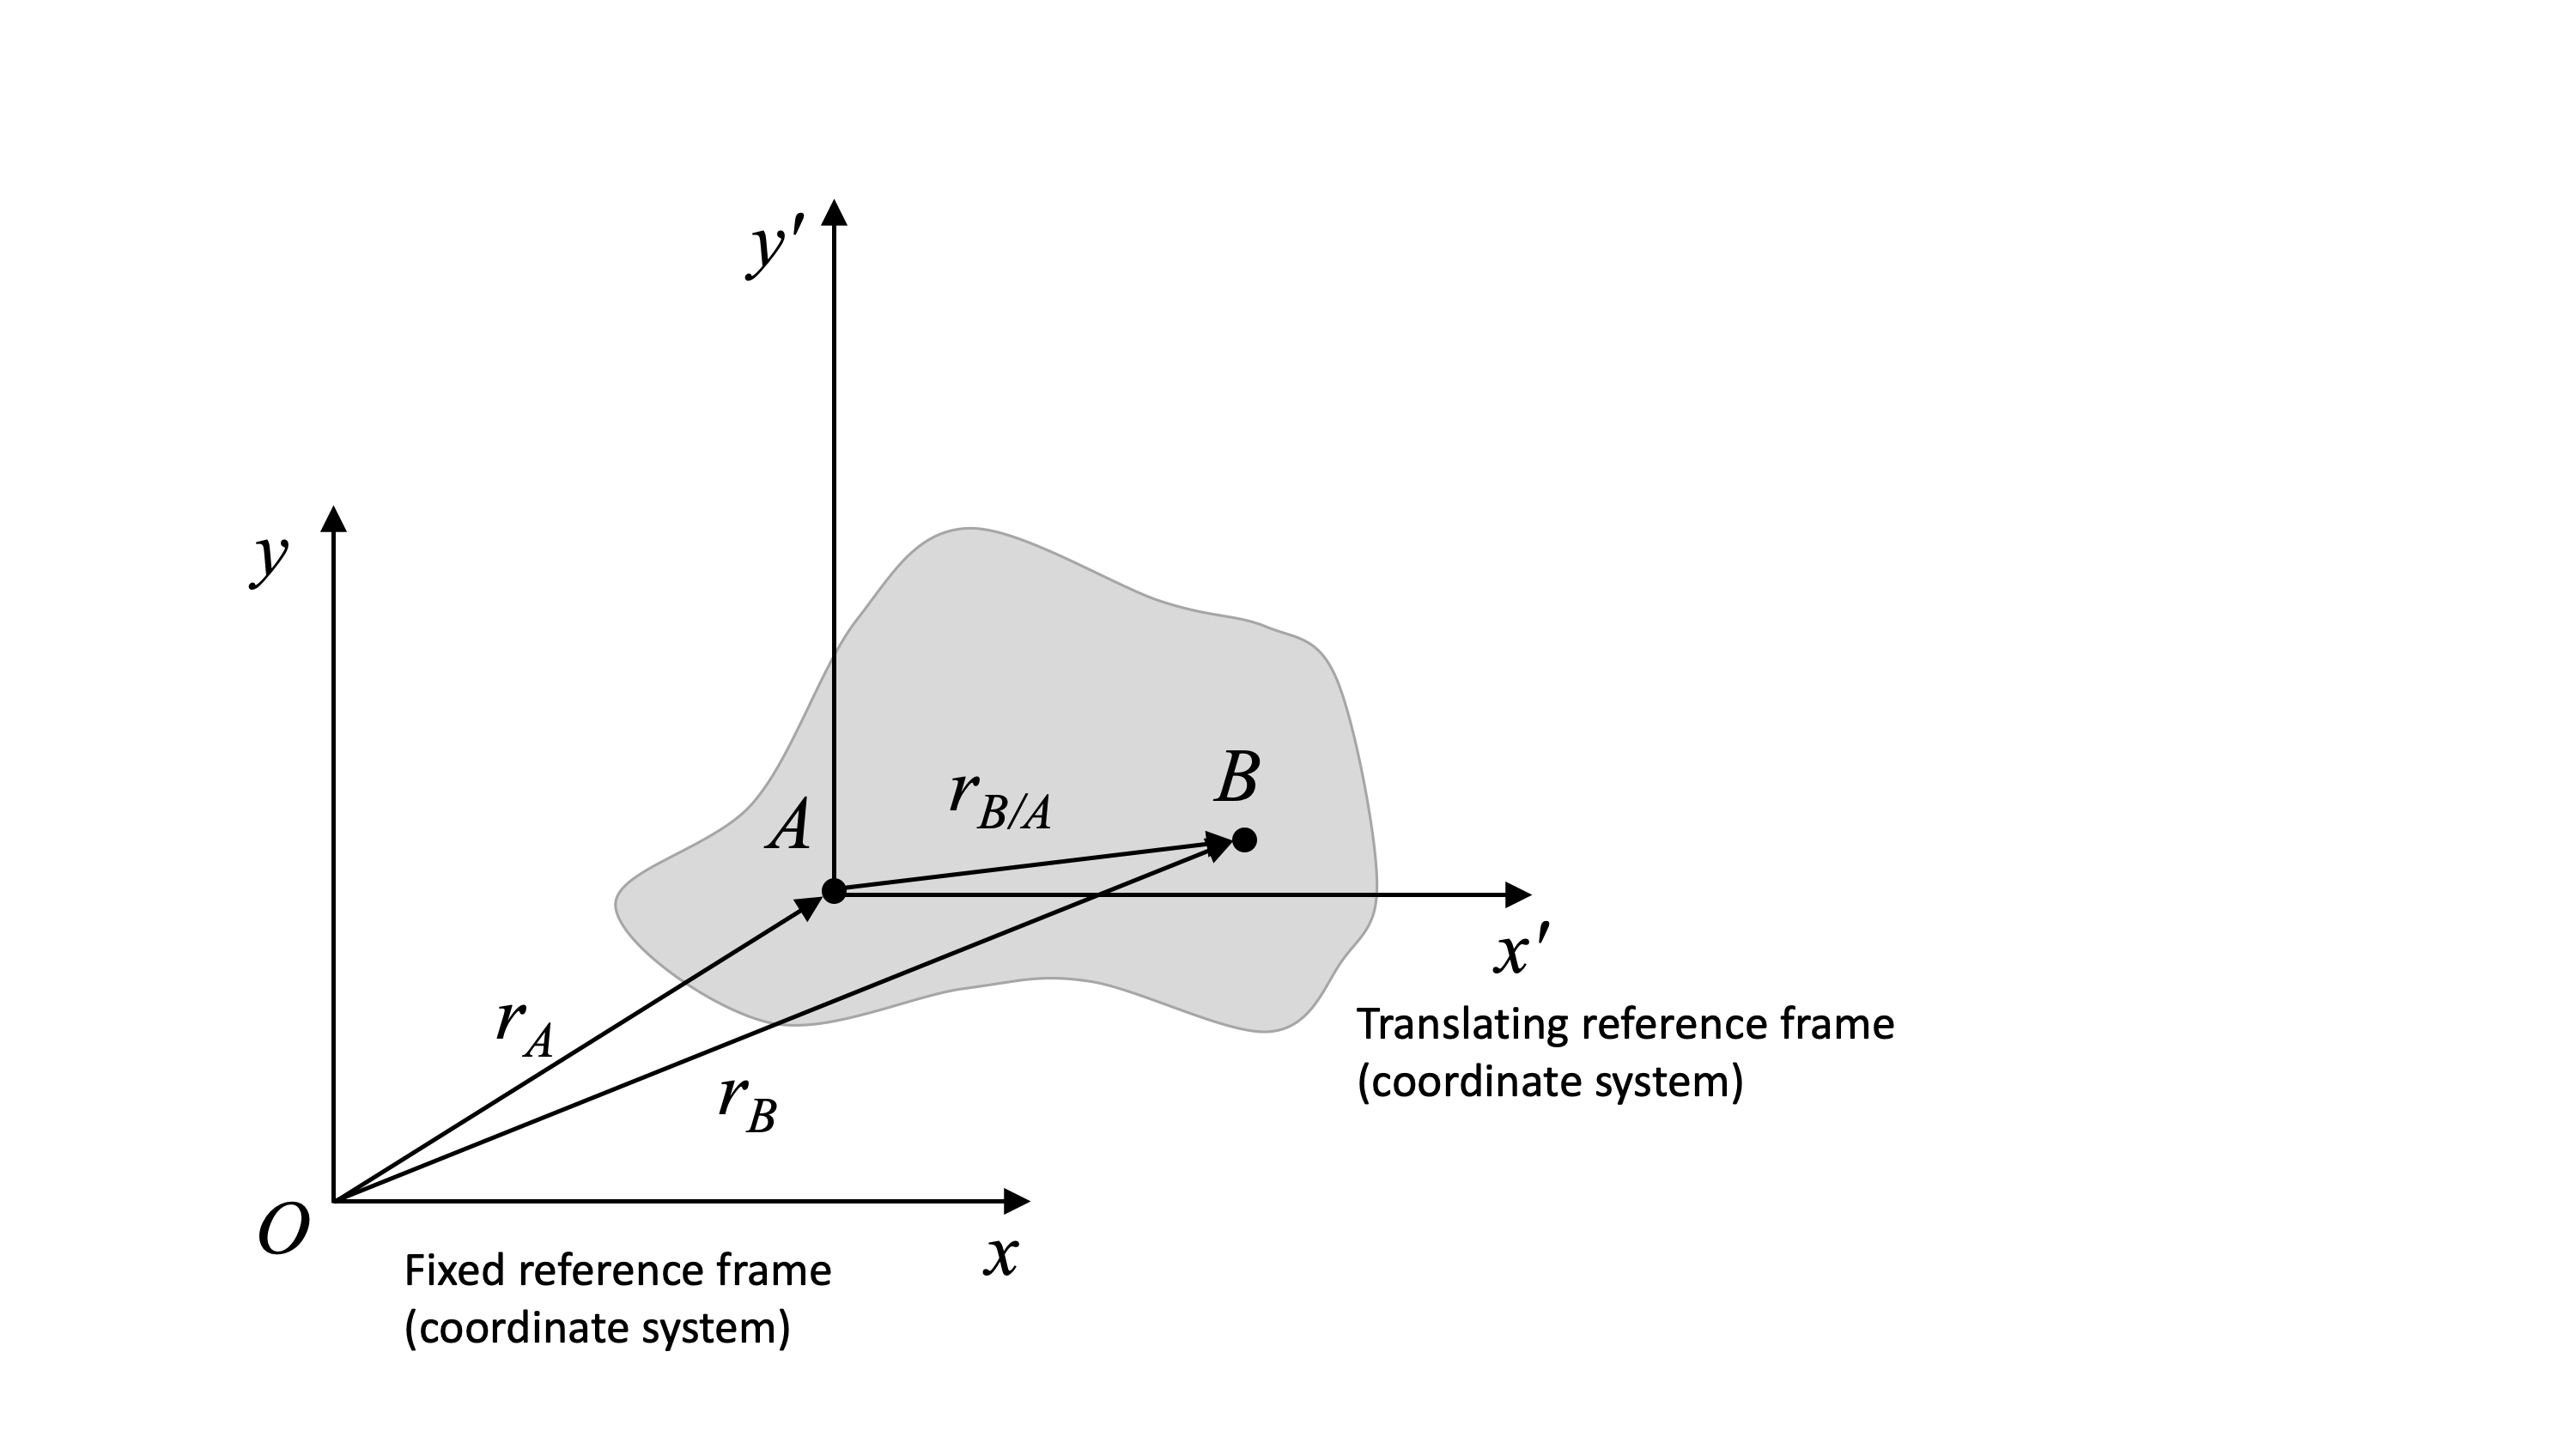
\includegraphics[trim={1cm 1cm 7cm 2.5cm},clip,width=1\textwidth, center]{Slide5} 
\end{minipage}


This is useful for the problems where rigid bodies are pinned to each other.   

\vspace*{11\baselineskip}

However, when we wish to analyze problems where rigid bodies are connected with sliding joints, or analyze two related but unconnected bodies, it is convenient to allow the moving frame to rotated as well as translate.  

In the case of a sliding joint on a rotating body, this allows the sliding motion to be described along a single coordinate direction.  

\vspace*{11\baselineskip}

In the case of general motion, this allows the motion of one object to be described with respect to an observer (e.g. a camera) fixed to another moving object that is both translating and rotating. 

\vspace*{11\baselineskip}

In such cases, we consider the frame on the moving body to be \textbf{translating and rotating} with the body. This will introduce extra terms in our formulations, in order to correctly account for the rotating frame.  

Consider a rigid body with frame $x'y'z'$ at point $A$. $x'y'z'$ translates and rotates with the body.  A bug, $B$, is crawling along the body:

\vspace*{24\baselineskip}

\begin{itemize}
\item The body and the frame $x'y'z'$ rotate with angular velocity $\bm{\Omega}$ and angular acceleration $\bm{\dot{\Omega}}$ in the $\bm{\hat{k}}$ direction. 
\item Viewed from the $x'y'z'$ frame, the bug, $B$, moves with velocity $\bm{(v_{B/A})_{x'y'z'}}$ (velocity of $B$ with respect to $A$, as viewed from the $x'y'z'$ frame). 
\item Point $A$ on the body and the frame $x'y'z'$ are translating with velocity $\bm{v_A}$ and acceleration $\bm{a_A}$. 
\end{itemize}

\vspace*{2\baselineskip}

\textbf{Describe the motion of point $B$:}

\textbf{Position (same as usual):} $\bm{r_B} = \bm{r_A} +  \bm{r_{B/A}}$ 

\textbf{Velocity:} since $\bm{r_{B/A}}$ is described in a reference frame that is rotating, $\bm{r_{B/A}} = \bm{r_x \hat{i'}} + \bm{r_y \hat{j'}}$ we need to differentiate both the magnitude and the direction of this vector.  

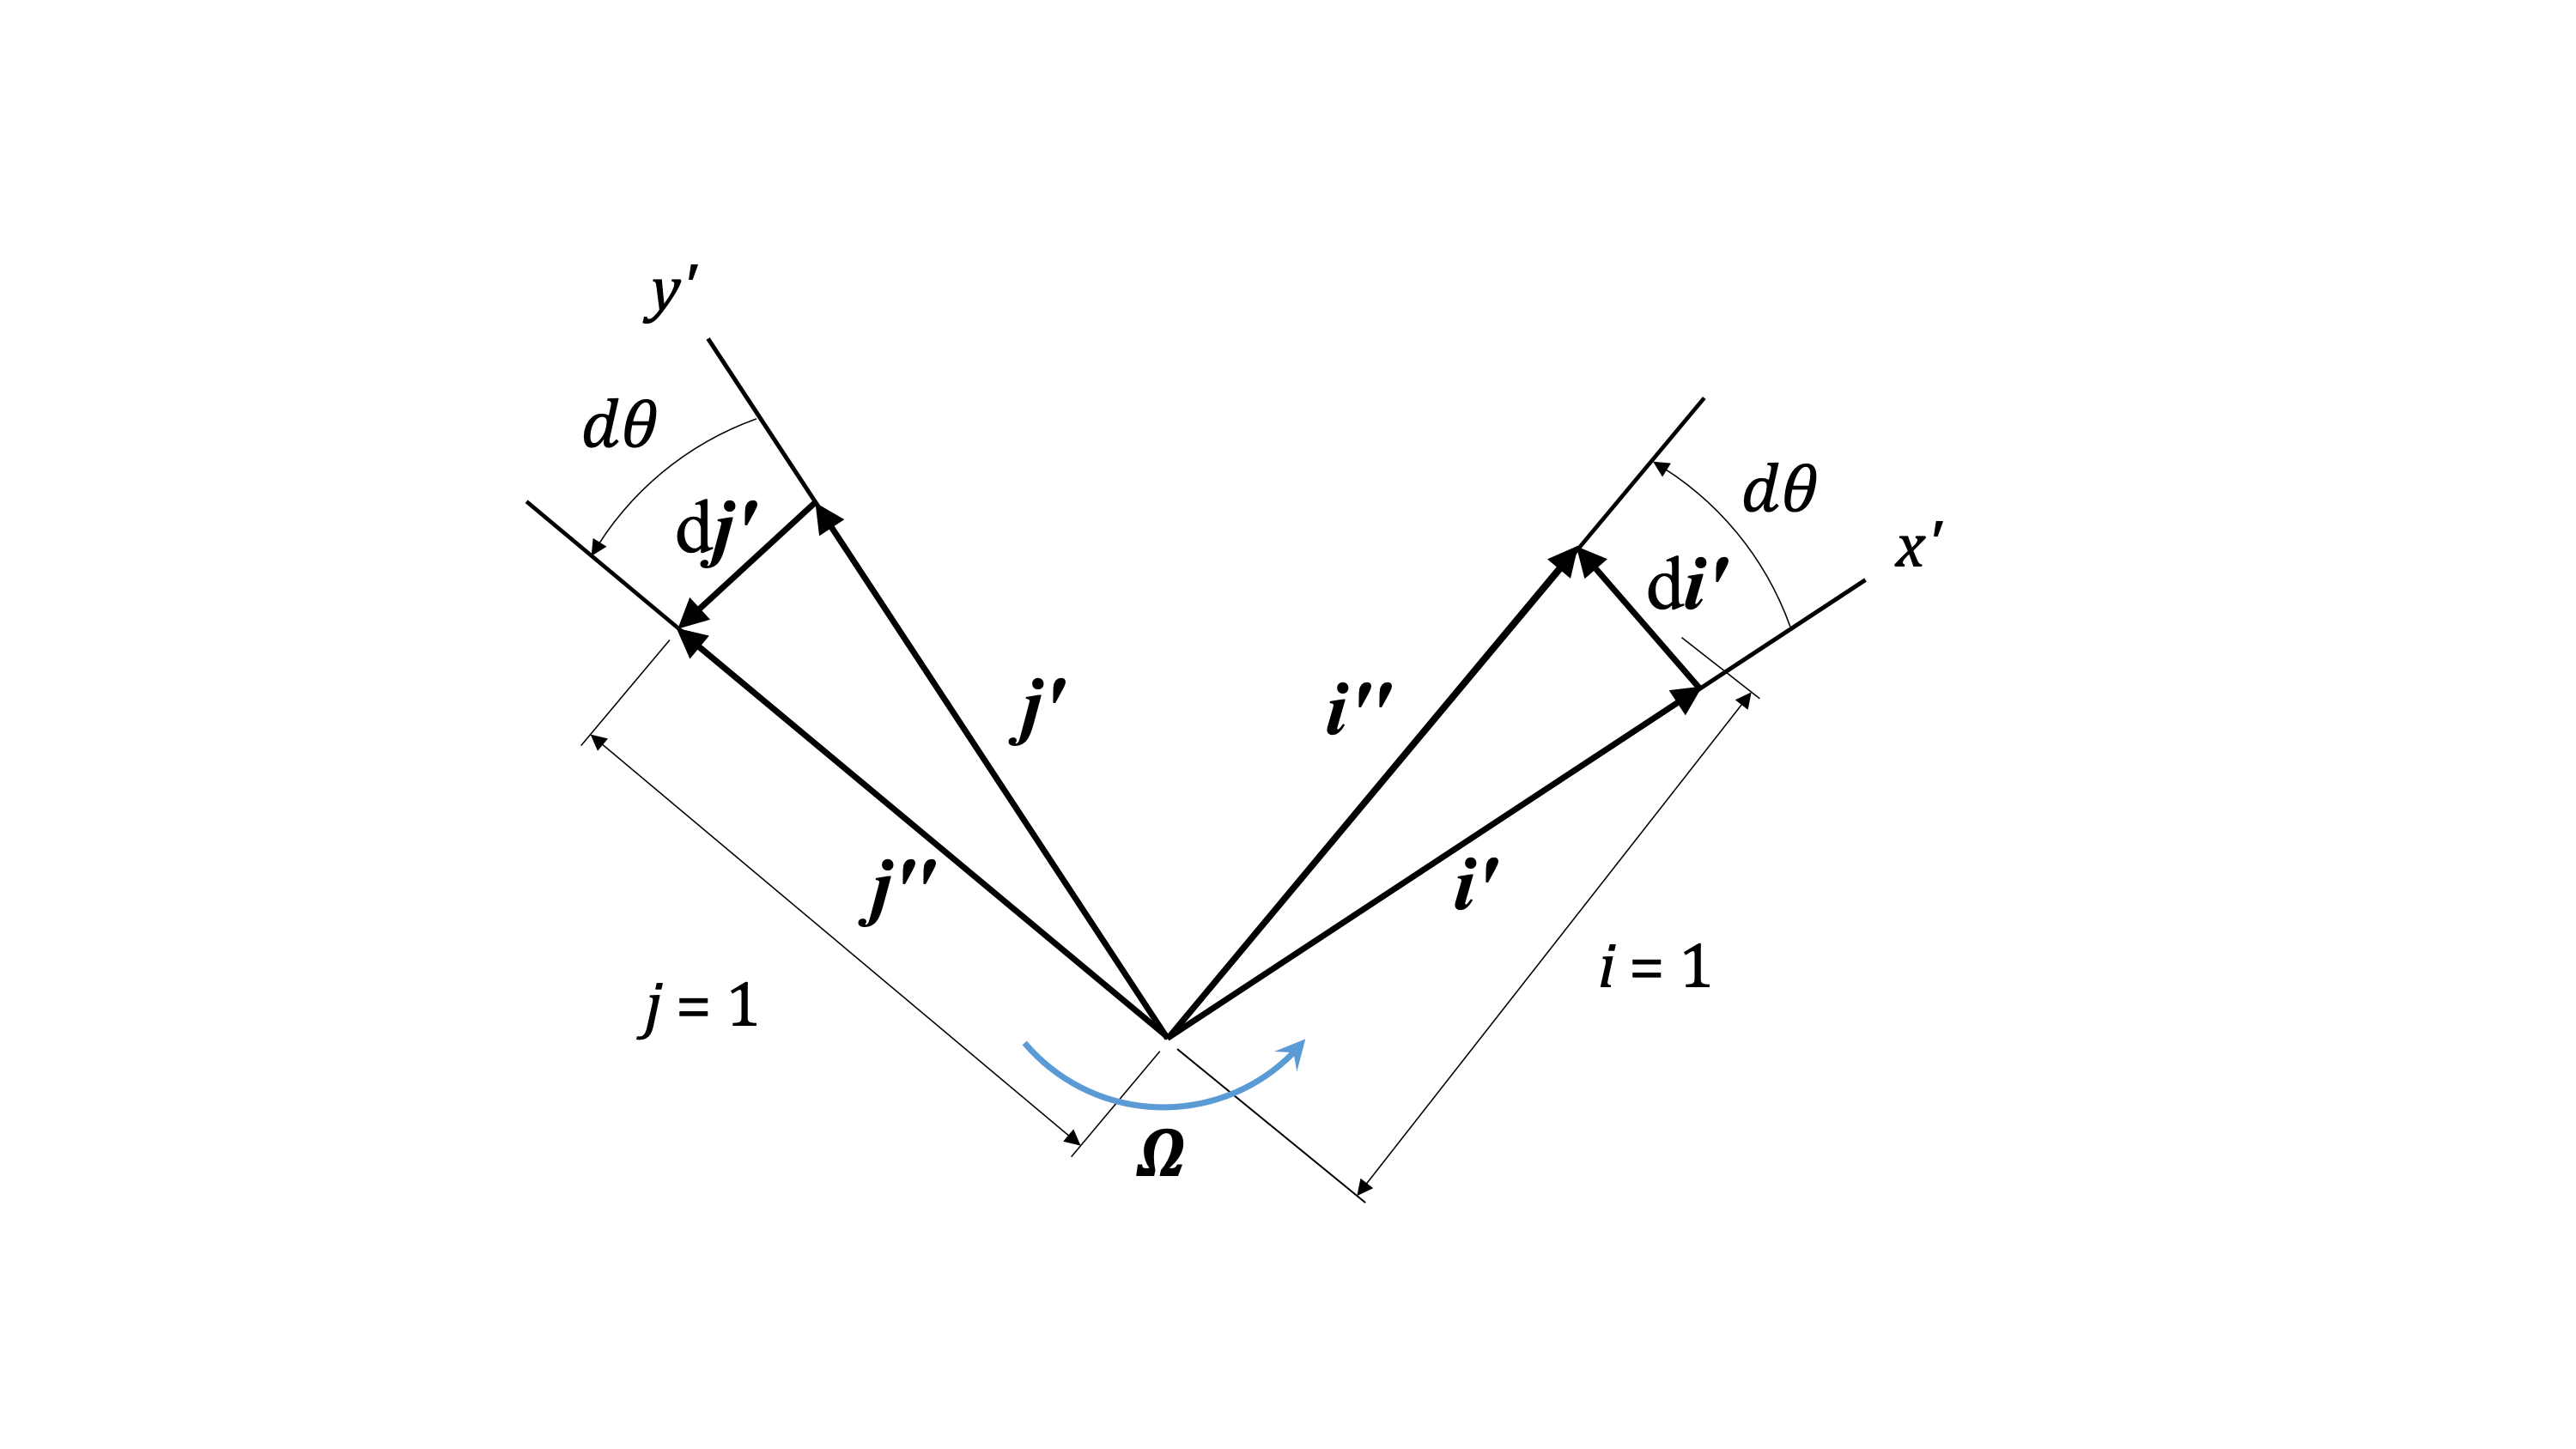
\includegraphics[trim={4cm 3cm 5cm 3cm},clip,width=0.6\textwidth, center]{Slide31} 


As before, when we see coordinate frames change direction due to rotation, we find that differentiating the direction components is effectively a cross product: 

\vspace*{8\baselineskip}

Thus we have:

\[
\frac {d \bm{r_{B/A}}} {dt} = (\bm{\dot{r_x} \hat{i'}} + \bm{\dot{r_y} \hat{j'}}) + \bm{\Omega} \times (\bm{r_x \hat{i'}} + \bm{{r_y} \hat{j'}})
\]

\vspace*{2\baselineskip}
\[
\frac {d \bm{r_{B/A}}} {dt} = \bm{(v_{B/A})_{x'y'z'}} + \bm{\Omega} \times \bm{r_{B/A}}
\]
\vspace*{2\baselineskip}

Thus:
\[
\bm{v_B} = \bm{v_A} + \bm{\Omega} \times \bm{r_{B/A}} + \bm{(v_{B/A})_{x'y'z'}}
\]

\newpage

\textbf{Acceleration:} Now, let's differentiate again:
\[
\bm{a_B} = \frac{d \bm{v_A}} {dt} + \frac{d \bm{\Omega}} {dt} \times \bm{r_{B/A}} + \bm{\Omega} \times \frac {d \bm{r_{B/A}}} {dt} + \frac{d\bm{(v_{B/A})_{x'y'z'}}}{dt}
\]

\vspace*{20\baselineskip}
\newpage

\section{Summary}

\begin{center}
\begin{tabu} to 1\textwidth {  | X[-2.5, c]  | X[1, l] | }
\hline
$\bm{a_A}$ & Absolute acceleration of point $A$ (referenced to a non-moving (fixed) frame) \\
\hline
$\bm{a_B}$ & Absolute acceleration of point $B$ (referenced to a non-moving (fixed) frame)  \\
\hline
$\bm{r_{B/A}}$ & Relative location of point $B$ w.r.t. $A$\\
\hline
$\bm{\Omega}$ & Angular velocity of rotating $x'y'z'$ frame w.r.t. fixed $XYZ$ frame. \\
\hline
$\bm{\dot{\Omega}}$ & Angular acceleration of rotating $x'y'z'$ frame w.r.t. fixed $XYZ$ frame. \\
\hline
$\bm{(v_{B/A})_{x'y'z'}}$ & Velocity of point $B$ w.r.t. $A$, as seen by an observer attached to the translating and rotating $x'y'z'$ frame. \\
\hline
$\bm{(a_{B/A})_{x'y'z'}}$ & Acceleration of point $B$ w.r.t. $A$, as seen by an observer attached to the translating and rotating $x'y'z'$ frame. \\
\hline
\end{tabu}
\end{center}

\vspace*{24\baselineskip}

VERY IMPORTANT NOTE: The components of all terms must be computed along the same $\bm{\hat{i}}$ and  $\bm{\hat{j}}$ directions. If the $XYZ$ and $x'y'z'$ frames are not aligned, you must pick ONE FRAME and express all terms along the \textbf{directions} of that ONE FRAME. 

Since the $x'y'z'$ frame rotates w.r.t. the $XYZ$ frame, it is likely that these two frames will not be aligned.  

\begin{center}
\begin{tabu} to 1\textwidth {  X[l]  }
$\bm{a_B}$\\
\\
$=$\\
\\
$\bm{a_A}$\\
\\
$+$\\
\\
$\bm{\dot{\Omega}} \times \bm{r_{B/A}}$\\
\\
$+$\\
\\
$\bm{\Omega} \times (\bm{\Omega} \times \bm{r_{B/A}})$\\
\\
$+$\\
\\
$2\bm{\Omega} \times \bm{(v_{B/A})_{x'y'z'}}$\\
\\
$+$\\
\\
$\bm{(a_{B/A})_{x'y'z'}}$\\
\end{tabu}
\end{center}

\subsection{Example}
Consider the quick return mechanism shown in the following figure. There are pin joints at $A$, $B$, $C$, $D$, and $E$.  Block $D$ slides along bar $AB$.  Block $E$ is constrained to slide horizontally.  The rotation of the crank $CD$ is the input motion and the output is the sliding motion of $E$. 

If the relative velocity of block $D$ with respect to the rotating bar $AB$, $\bm{(v_{D/A})_{x'y'z'}}$ is a constant $1 \, m/s$, find the angular velocities and angular accelerations of bars $AB$ and $CD$.  

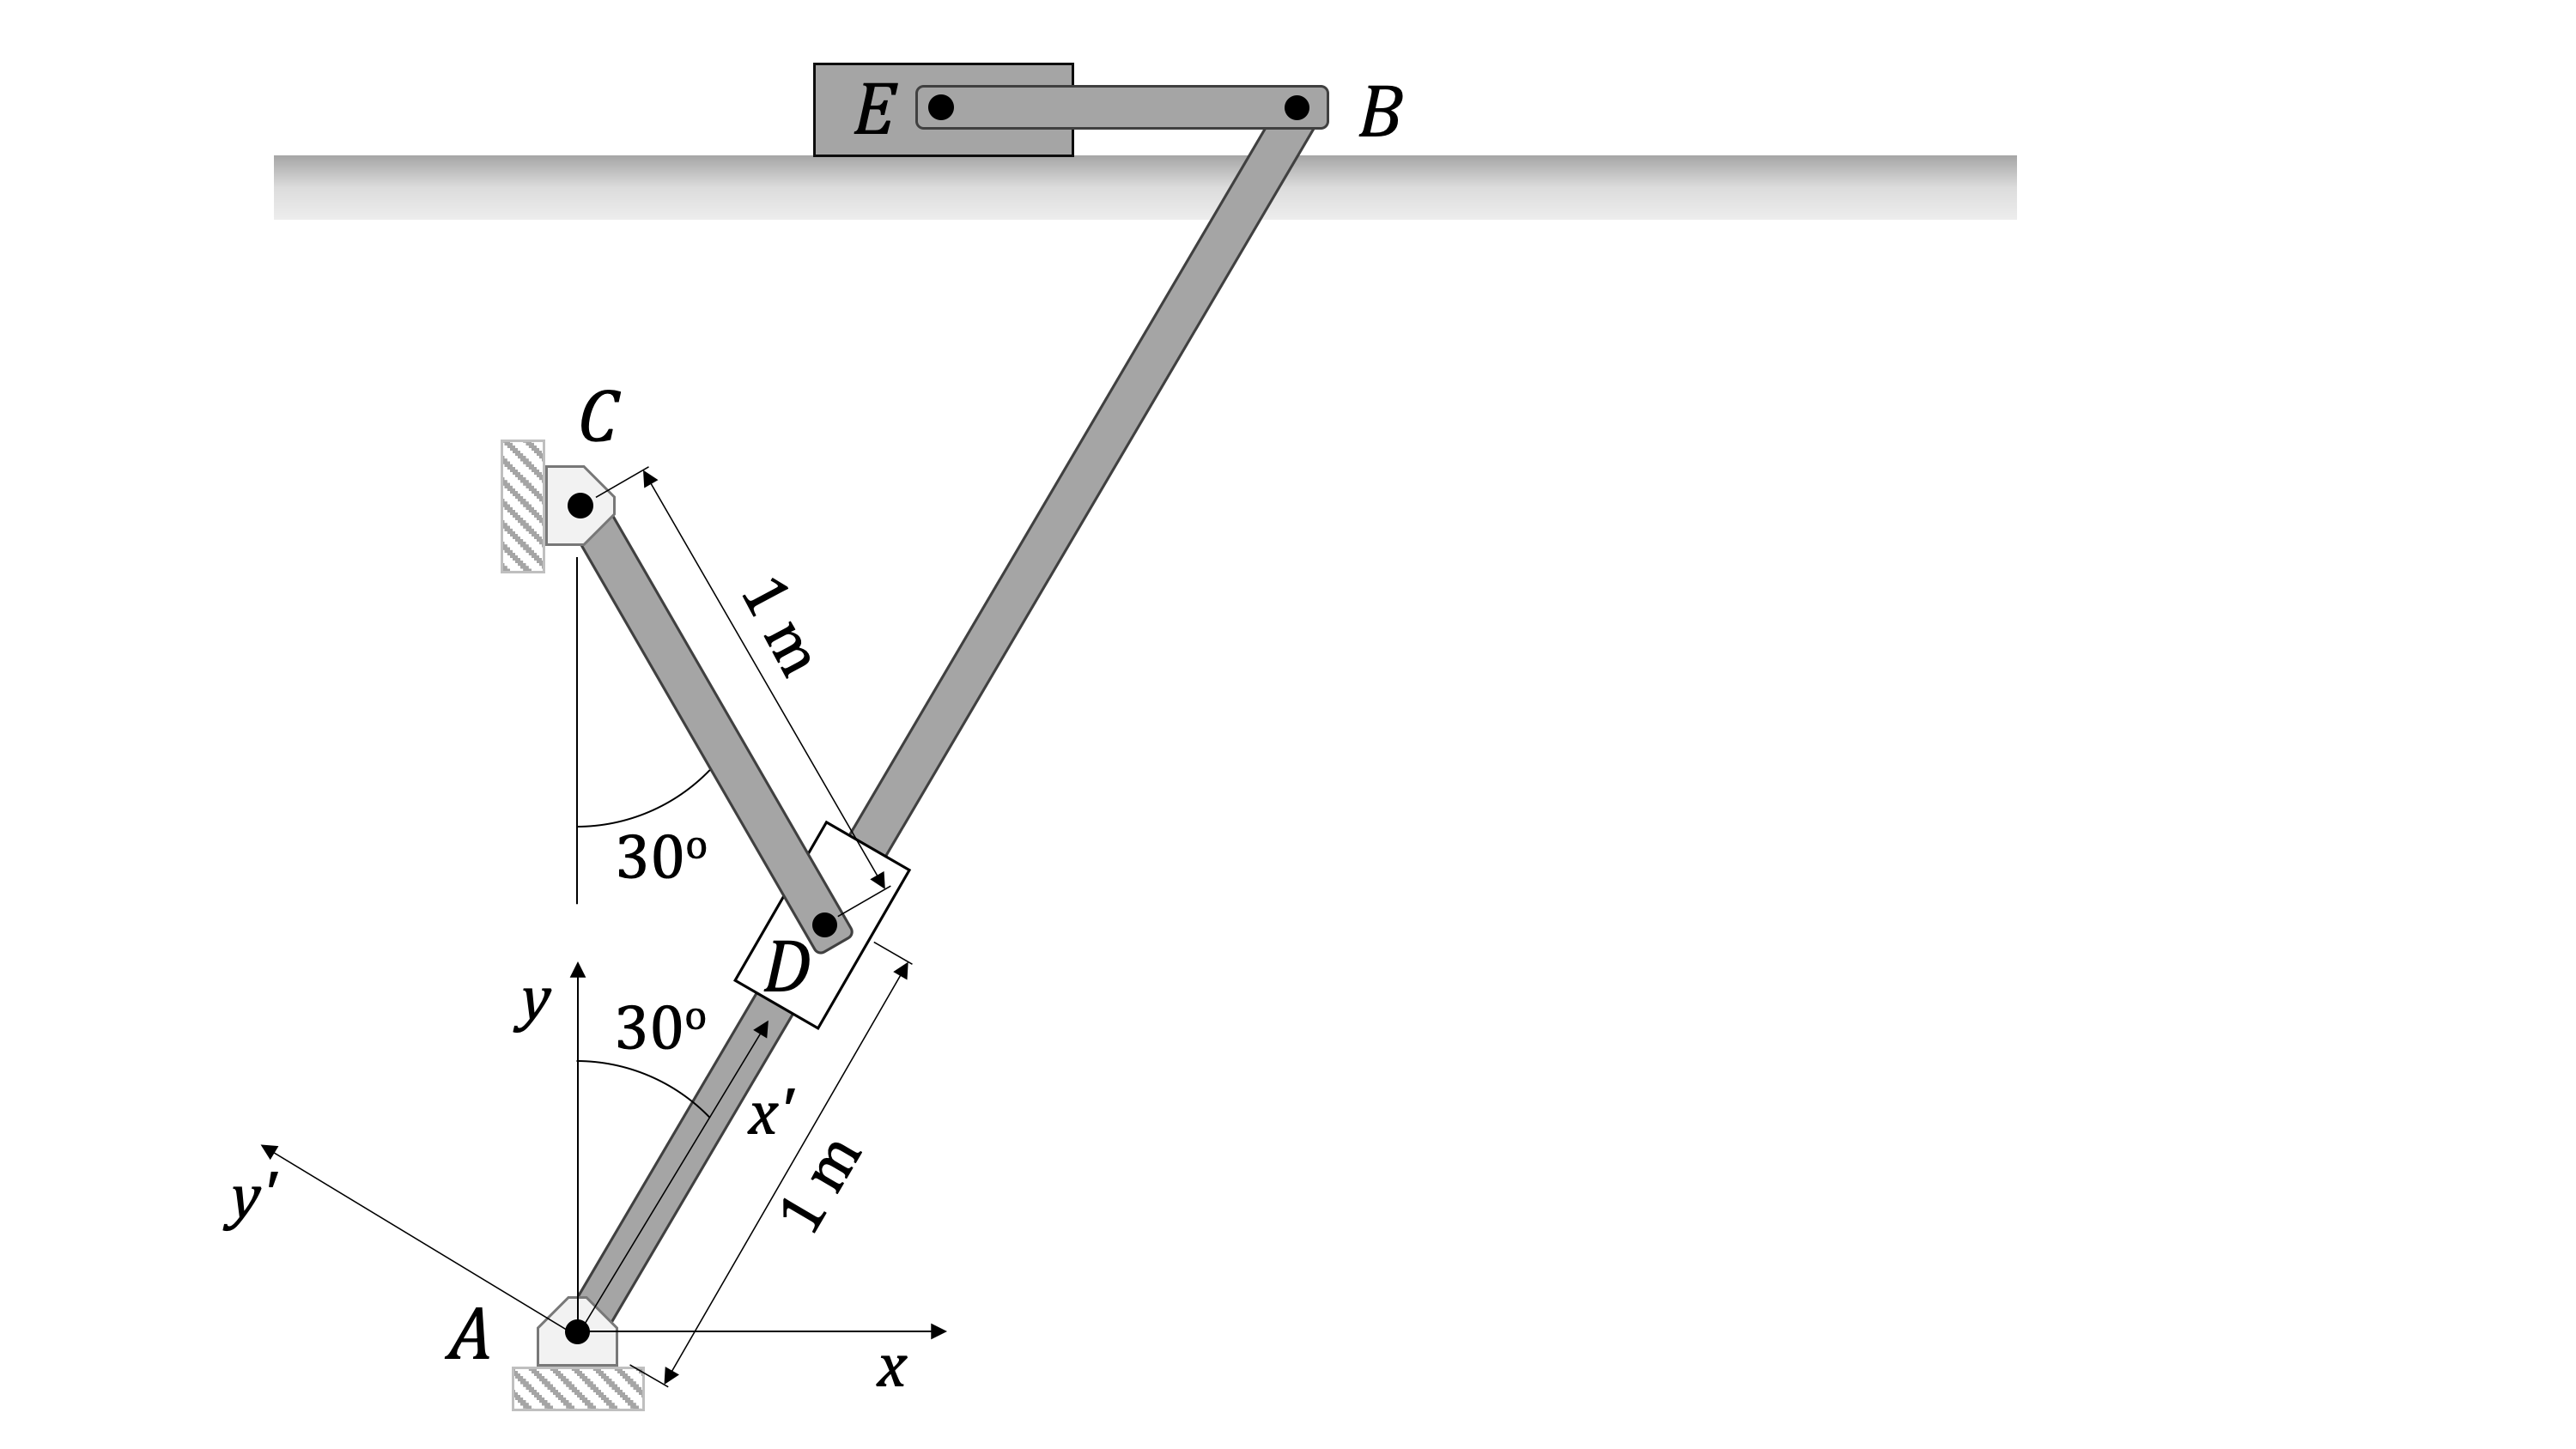
\includegraphics[trim={1cm 0cm 10cm 0cm},clip,width=0.9\textwidth, left]{Slide32} 

\vspace*{20\baselineskip}
\newpage
(Example continued)

\chapter{L7: Absolute General Plane Motion}
Reading

\section{Objective}
To relate rectilinear point motion with rotational motion on a rigid body. 

\section{Method}
There are no "new equations". Use known geometric relationships. Try to relate angular rotation of a line fixed to the body, $\theta(t)$, $\dot{\theta(t)}$, $\ddot{\theta(t)}$, to the rectilinear (straight line) location of a point specified by a parameterized path, e.g.: $s=f(\theta)$. 

\begin{enumerate}
\item Draw it!
\item For a point $P$ (translational point), define a position coordinate, $s$. 
\item Draw a line through the body at reference angle $\theta$. 
\item Using geometry/trigonometry, find a parameterized relationship, $s=f(\theta)$. 
\item Use time derivatives to relate: 
\end{enumerate}

\[ v = f'(\theta) \dot{\theta} = f'(\theta) \omega
\]
\[a = f''(\theta) \dot{\theta}^2 + f'(\theta) \alpha
\]

\subsection{Example}
Consider the robotic grinder. Find the position, velocity and acceleration of the grinding wheel as a function of the angles $\theta_A$ and $\theta_B$ and their derivatives.  

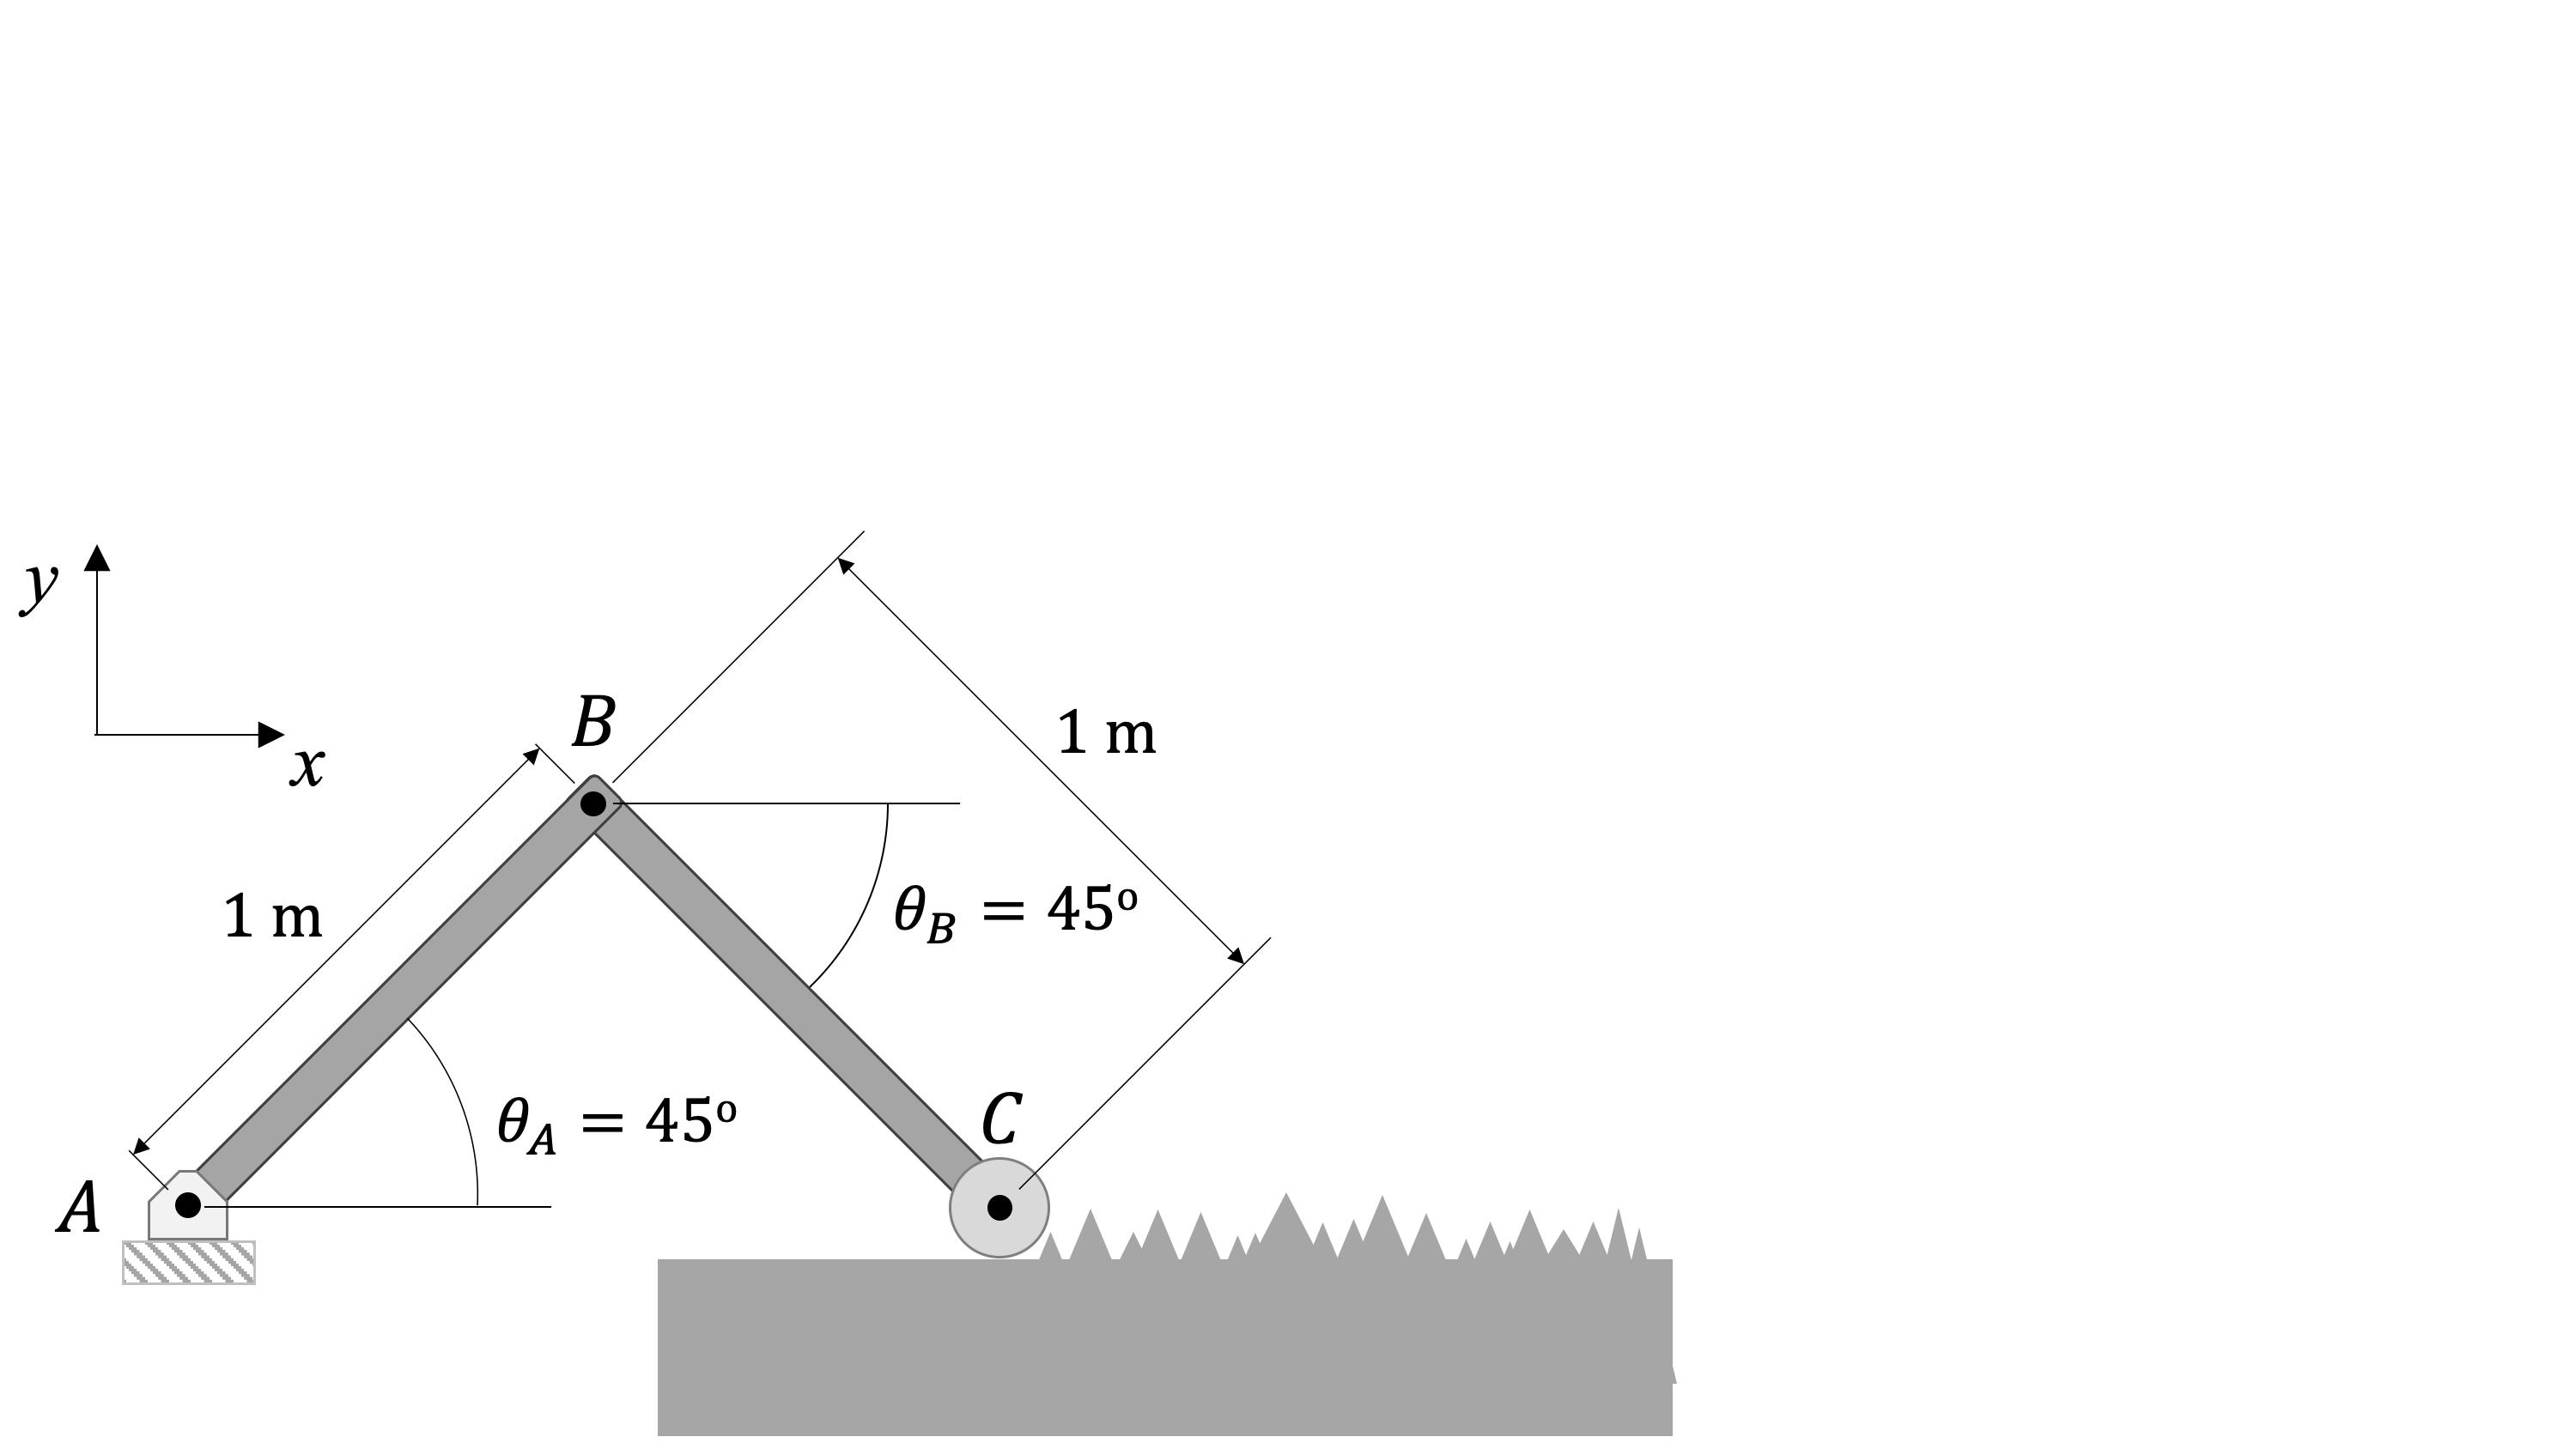
\includegraphics[trim={0cm 0cm 12cm 7cm},clip,width=0.6\textwidth, left]{Slide29} 

\newpage

\section{Summary}
Absolute general plane motion analysis can provide a quick, ad-hoc solution for 2-link problems with constrained motion.  For more than 2 links, however, the math and geometry can get pretty ugly.  Better to use relative frames. 

Pros:
\begin{itemize}
\item Can yield a fast solution
\end{itemize}

Cons:
\begin{itemize}
\item Relationship may not be obvious
\item If relationship is wrong, you've blown the whole problem (and it may be hard for the marker to give you part marks, unless they can understand what you have done)
\item Method cannot easily be checked by vector analysis
\end{itemize}

\subsection{Example}
Point $A$ at the end of a bar is moving downward in a slot with a constant velocity $\bm{v_A}$.  Find the angular velocity and angular acceleration of the bar as a function of the vertical position of $A$, $y$. 

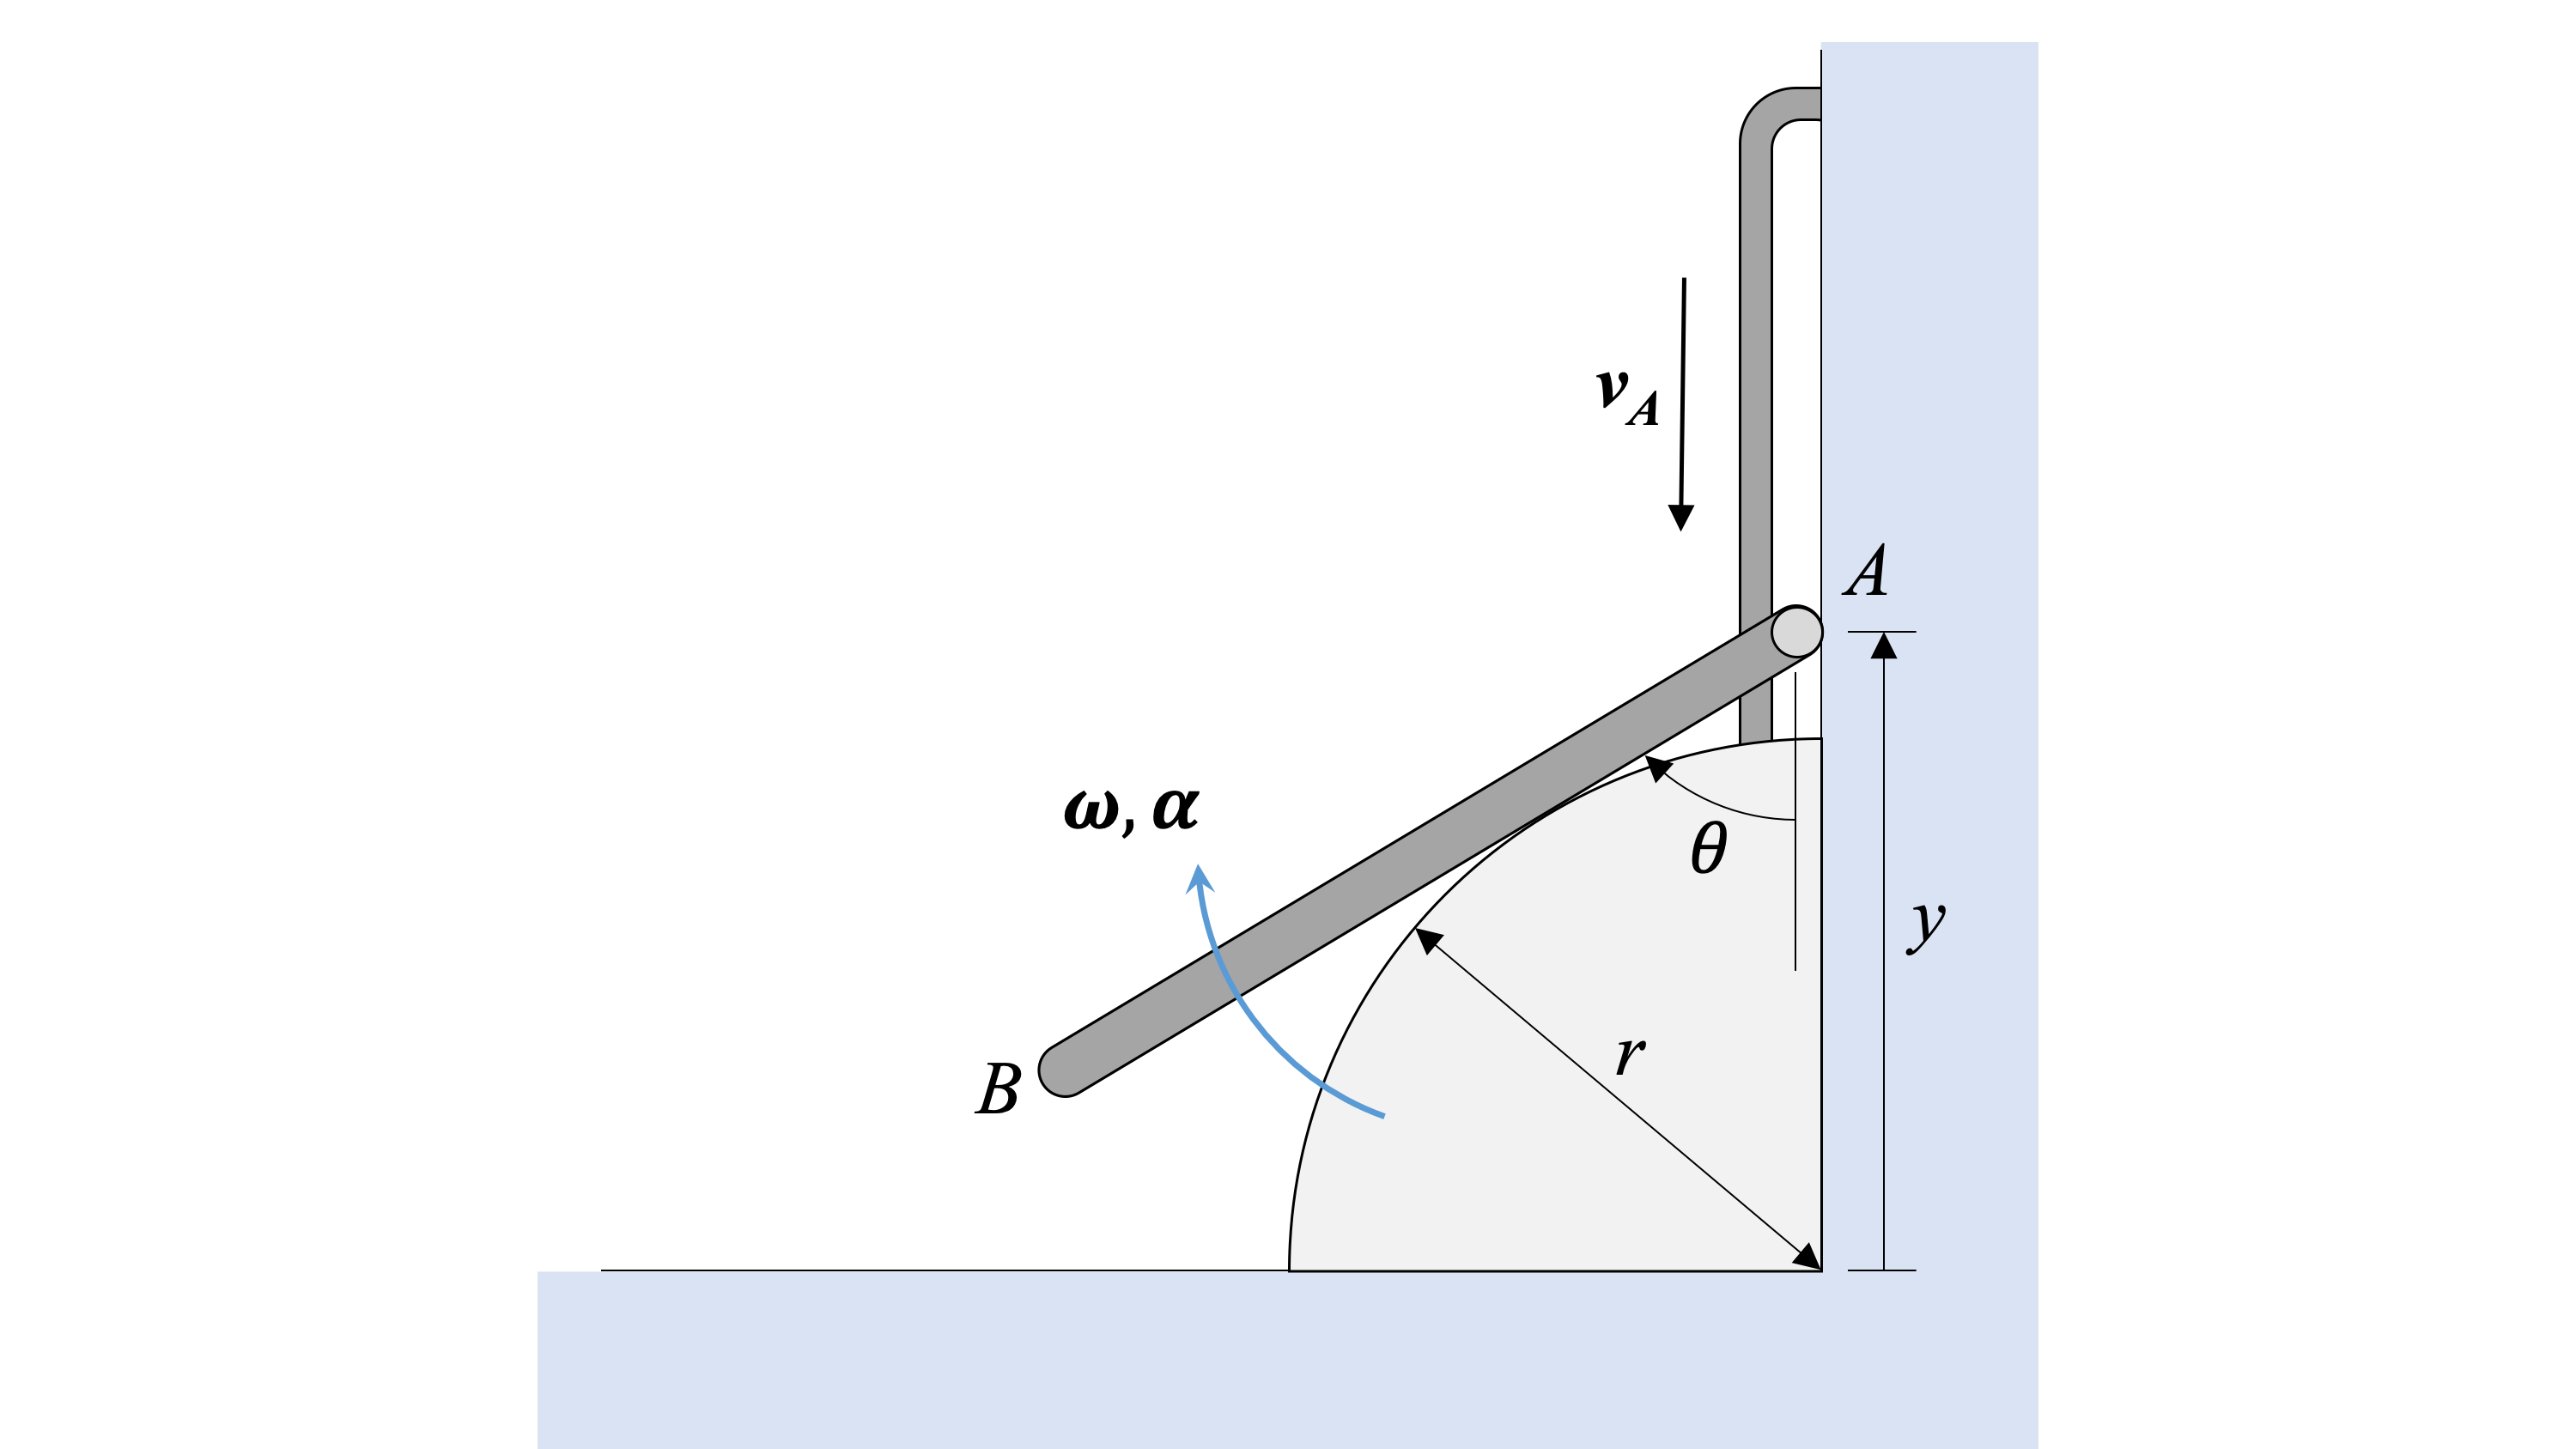
\includegraphics[trim={11cm 0cm 7cm 0cm},clip,width=0.35\textwidth, left]{Slide34} 
\newpage
(Example continued)
\newpage
(Example continued)
\newpage
(Example continued)
\newpage
(Example continued)

\chapter{L8/L9: Centroids, Centres of Mass, Moments of Inertia, and Mass Moments of Inertia}
Readings

\section{Objective}
To describe what the Centroids, Centres of Mass, Moments of Inertia and Mass Moments of Inertia are, to see examples where these quantities are used, and to compute them.  

\section{Centroids}
The centroid of a region can be thought of as the region’s \textbf{balance point} or \textbf{point of symmetry} of the object.  The centroid is located at the intersection of the \textbf{axes of symmetry} of the body.  

\newpage

Consider a uniform mass distributed over a planar surface: if placed on a pivot at the centroid, the surface would be balanced on the pivot. (Centroid located at $(x_C, y_C)$).

\vspace*{10\baselineskip}
If we identify the centroid by the letter $C$, and we consider each portion, $\Delta A_i$, of the area (where $\displaystyle \sum_{i} \Delta A_i = A$, we can find the $x,y$ location of the centroid as follows:

\[
x_C = \frac{\displaystyle \sum_{i} x_i \Delta A_i}{\displaystyle \sum_{i} \Delta A_i} = \frac{\displaystyle \sum_{i} x_i \Delta A_i}{A} \hspace{1cm} y_C = \frac{\displaystyle \sum_{i} y_i \Delta A_i}{\displaystyle \sum_{i} \Delta A_i} = \frac{\displaystyle \sum_{i} y_i \Delta A_i}{A} 
\]

In integral form this is written as:
\[
x_C = \frac{\displaystyle  \iint_A x dA }{\displaystyle \iint_A dA} = \frac{\displaystyle \int_{x_1}^{{x_2}} \int_{y_1(t)}^{{y_2(t)}} x dy dx}{\displaystyle \int_{x_1}^{{x_2}} \int_{y_1(t)}^{{y_2(t)}} dy dx} = \frac{\displaystyle \int_{x_1}^{{x_2}} x dx \int_{y_1(t)}^{{y_2(t)}} dy}{\displaystyle \int_{x_1}^{{x_2}} dx \int_{y_1(t)}^{{y_2(t)}} dy} = \frac{\displaystyle \int_{x_1}^{{x_2}} x dx [y_2(x) - y_1(x)]}{\displaystyle \int_{x_1}^{{x_2}} dx [y_2(x) - y_1(x)]}
\]

\[
x_C =\frac{\displaystyle \int_{x_1}^{{x_2}} x [y_2(x) - y_1(x)] dx}{A}
\]

\vspace*{10\baselineskip}

Note: the term $\displaystyle  \iint x dA$ is called the \textbf{first moment of area} about the x-axis (i.e. $x^1$). 

Similarly, 
\[
y_C = \frac{\displaystyle \iint_A y dA }{\displaystyle \iint_A dA}=\frac{\displaystyle \int_{y_1}^{{y_2}} y [x_2(y) - x_1(y)] dy}{A}
\]

If we think of $\bm{r}$ as a vector, $\bm{r}=(x,y)$, we can write the location of the centroid as:

\[
\bm{r_C} =\frac{\displaystyle  \sum_{i} \bm{r_i} \Delta A_i}{\displaystyle \sum_{i} \Delta A_i} = \frac{\displaystyle  \sum_{i} \bm{r_i} \Delta A_i}{A} 
\]

Or, in integral form: 

\[
\bm{r_C} =\frac{\displaystyle \iint_A \bm{r_i} dA}{\displaystyle \iint_A dA} = \frac{\displaystyle  \iint_A \bm{r_i} dA}{A} 
\]

where the the location of $\bm{r_C} =(x_C,y_C)$ can be computed using the equations for $x_C$ and $y_C$ above. 

NOTE:  for centroids of 3D objects, we compute $\bm{r_C} =(x_C,y_C,z_C)$ in a similar manner, except instead of considering area, we consider volume, $dV=dxdydz$.  

\subsection{Example}
Compute the location of the centroid, $\bm{r_C}$, for the shapes shown.

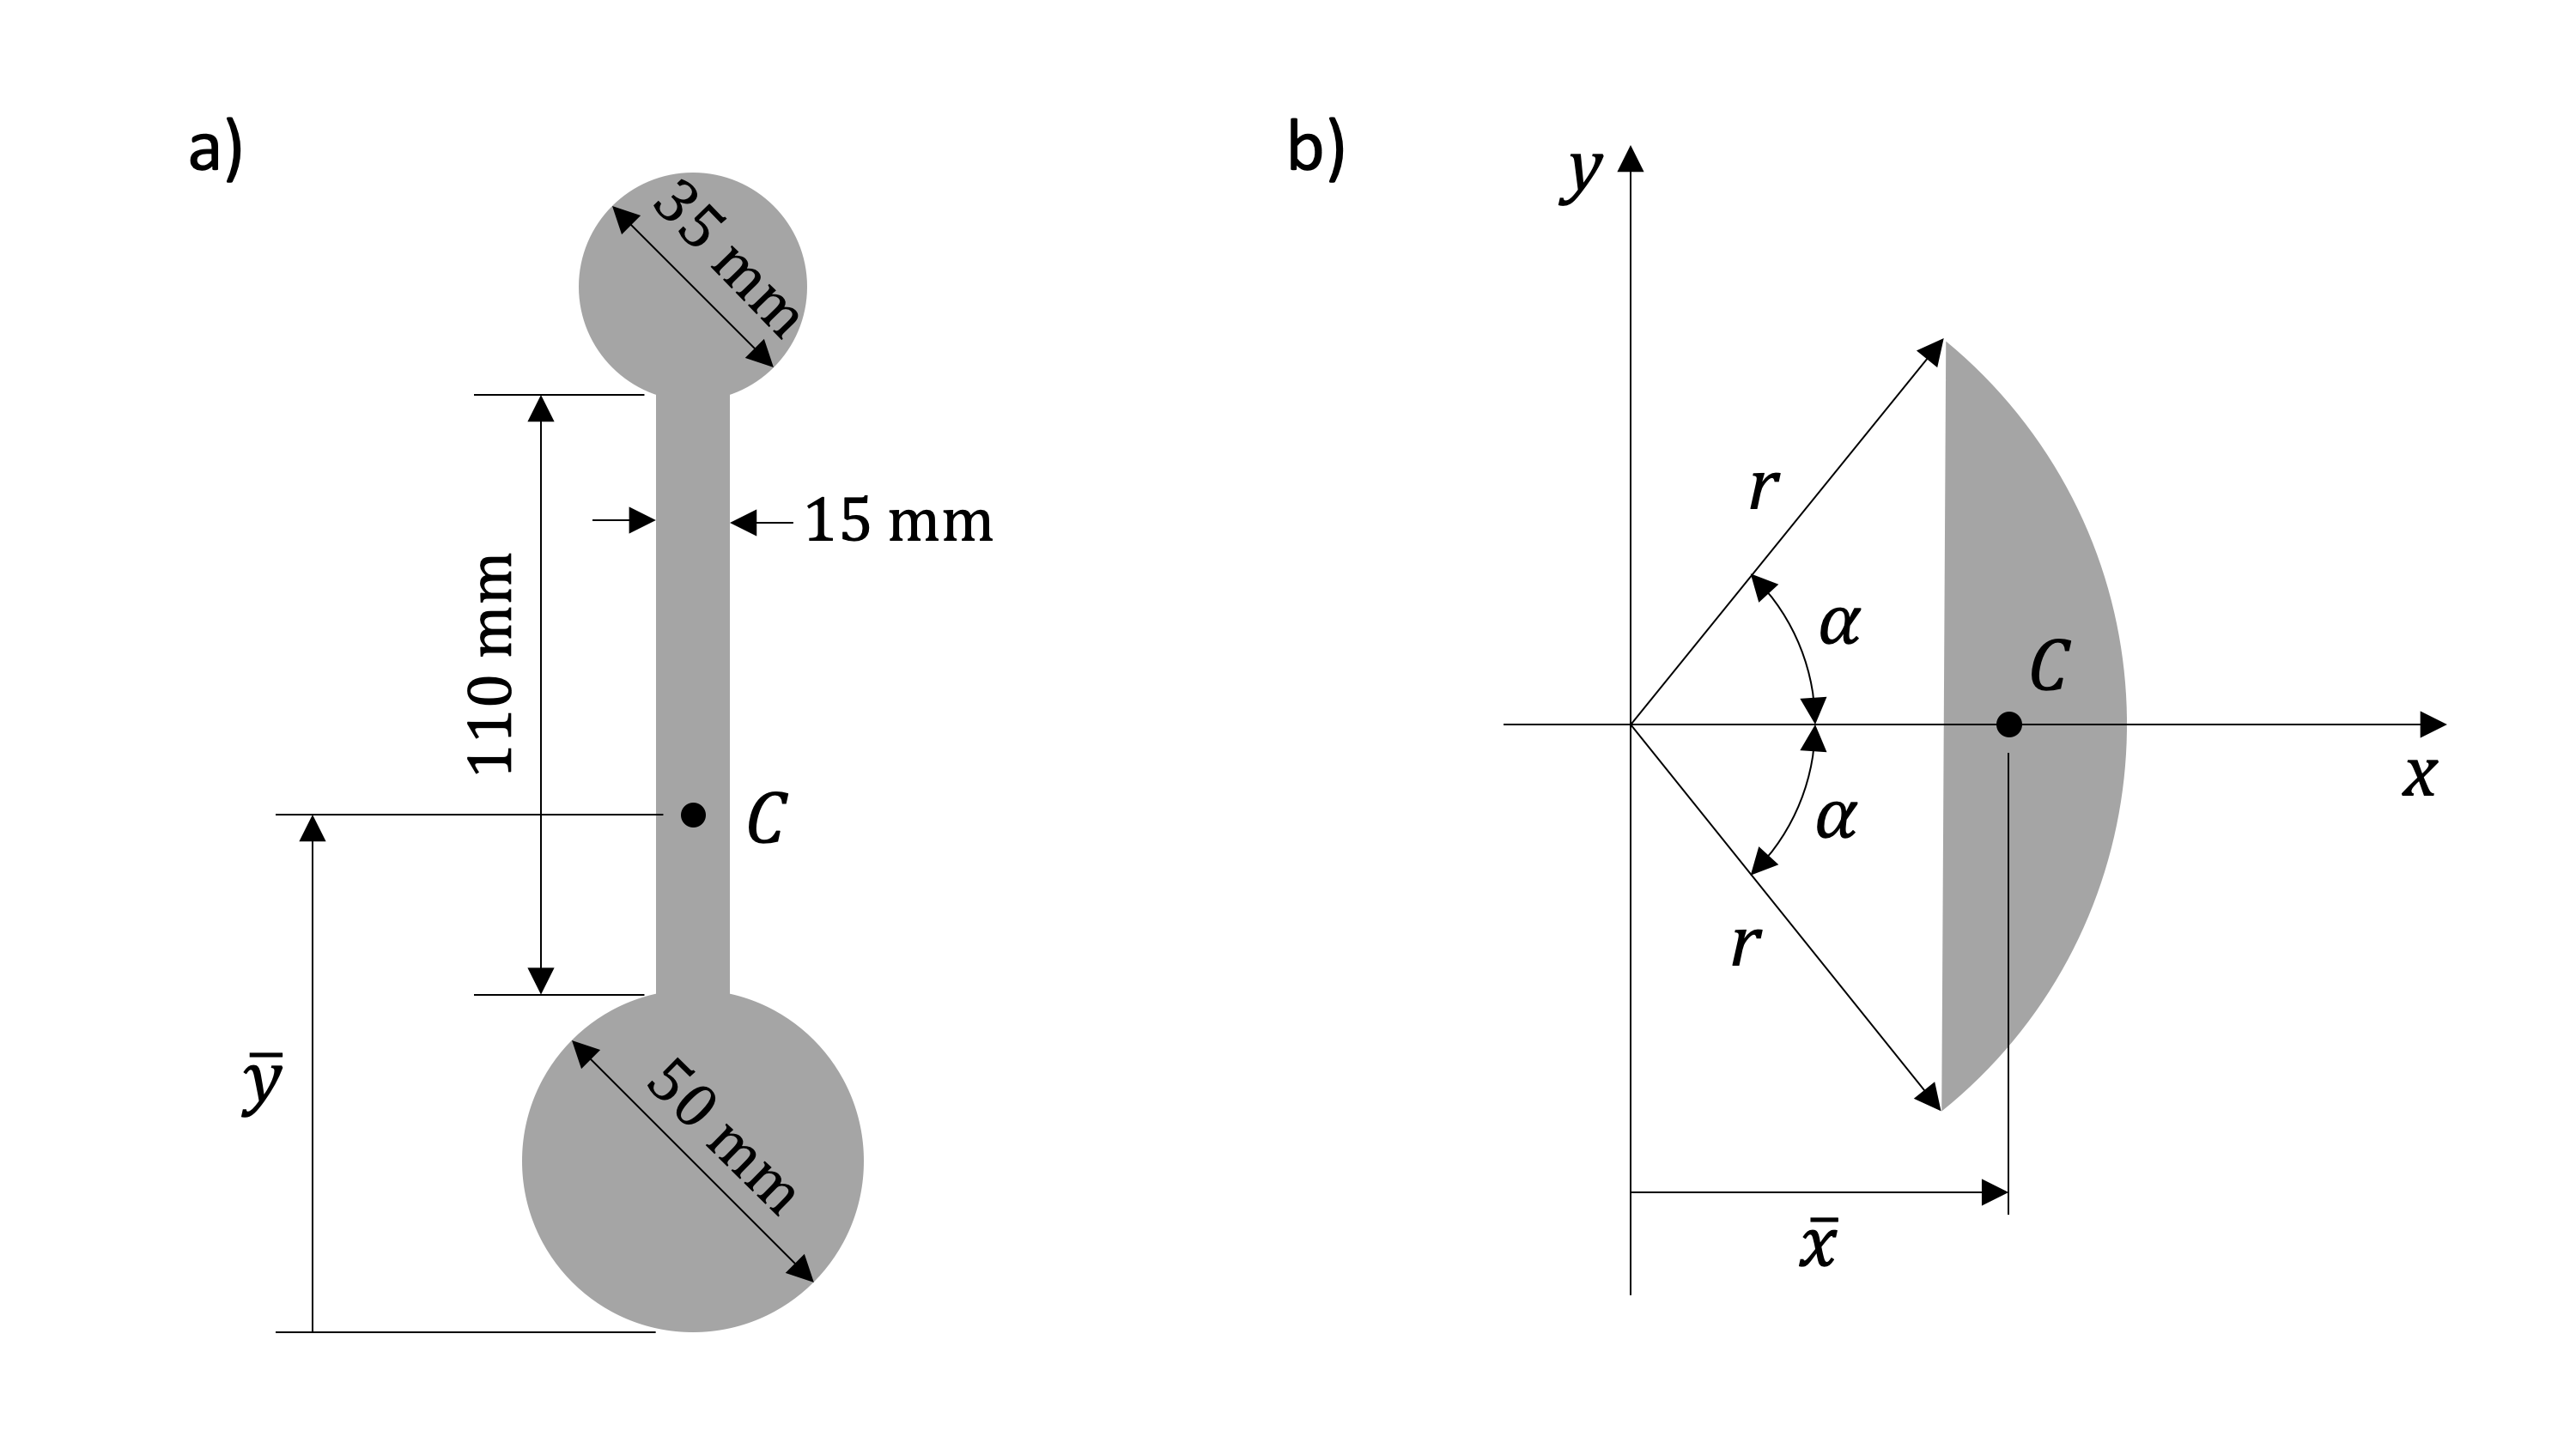
\includegraphics[trim={1cm 0cm 1cm 0cm},clip,width=0.75\textwidth, left]{Slide36}
\newpage

(Example continued)

\newpage

\section{Applications of Centroids}
For a uniform distributed load over a surface:  e.g. a uniform pressure distribution, or a uniformly distributed normal load, the effective force acts through the centroid of the surface.  

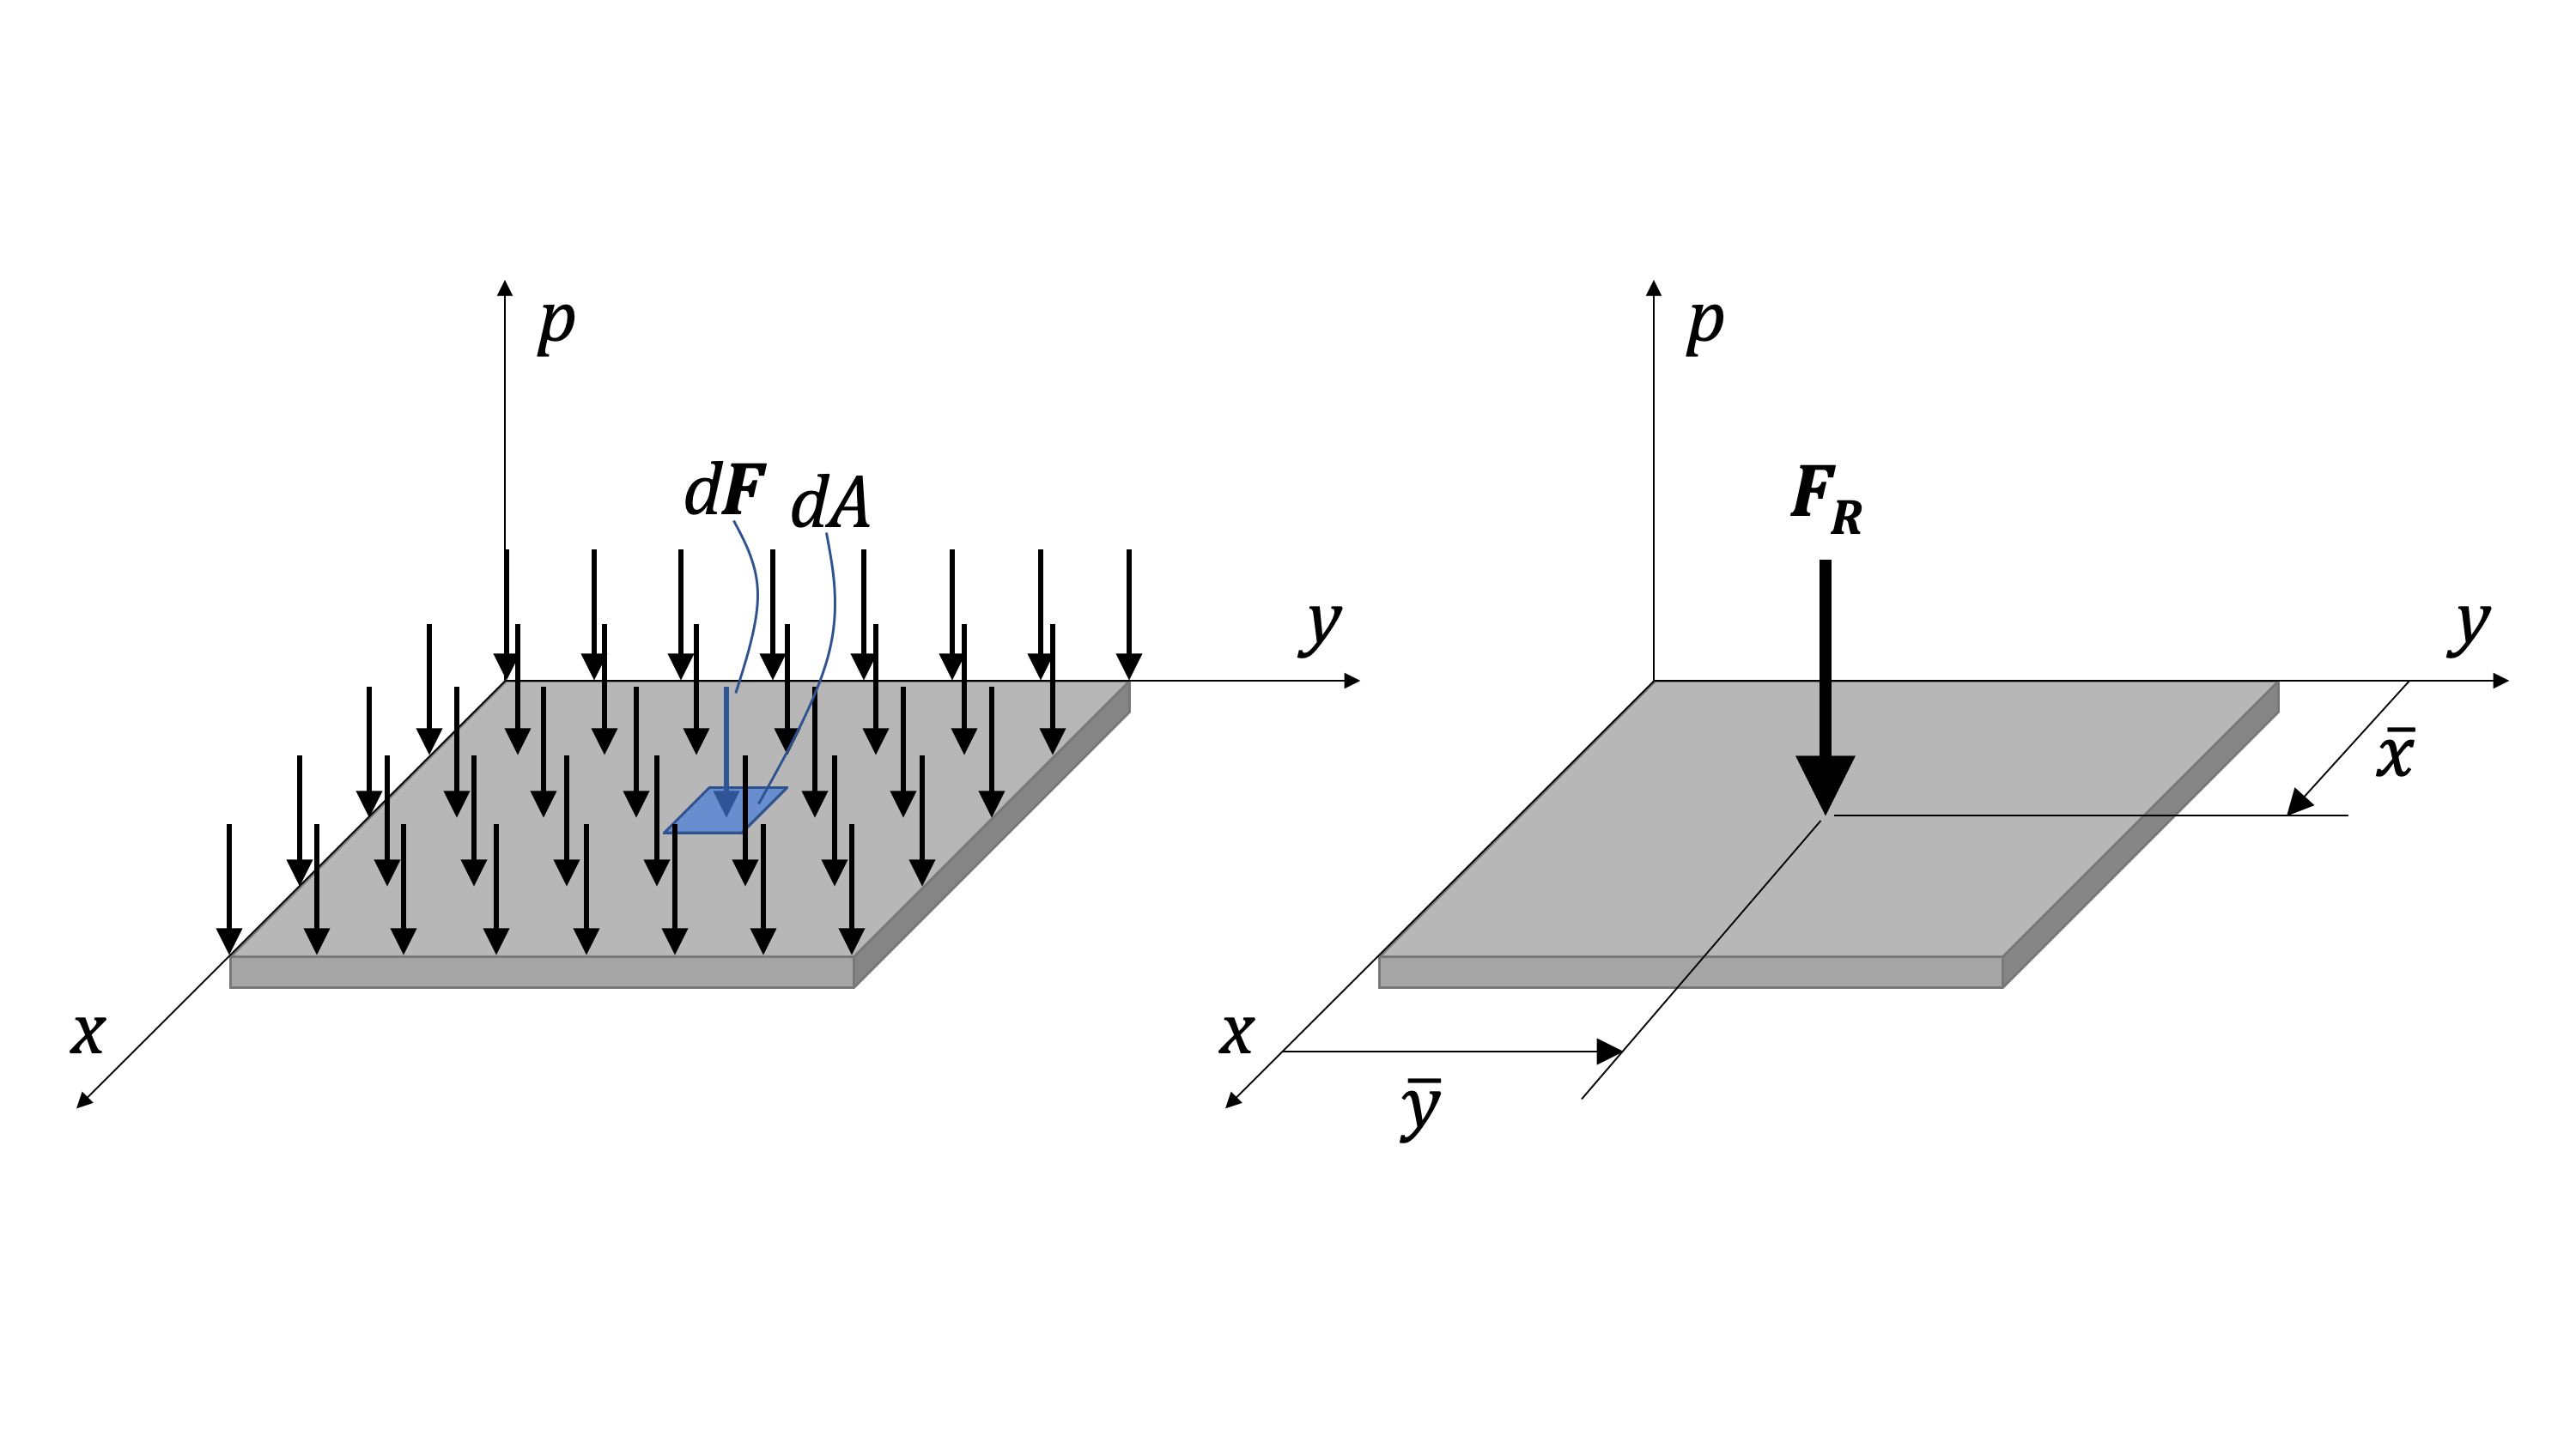
\includegraphics[trim={0cm 2cm 0cm 2cm},clip,width=0.9\textwidth,center]{Slide37} 

For a non-uniform pressure or stress distribution, the resultant force acts through the centroid of the distribution:

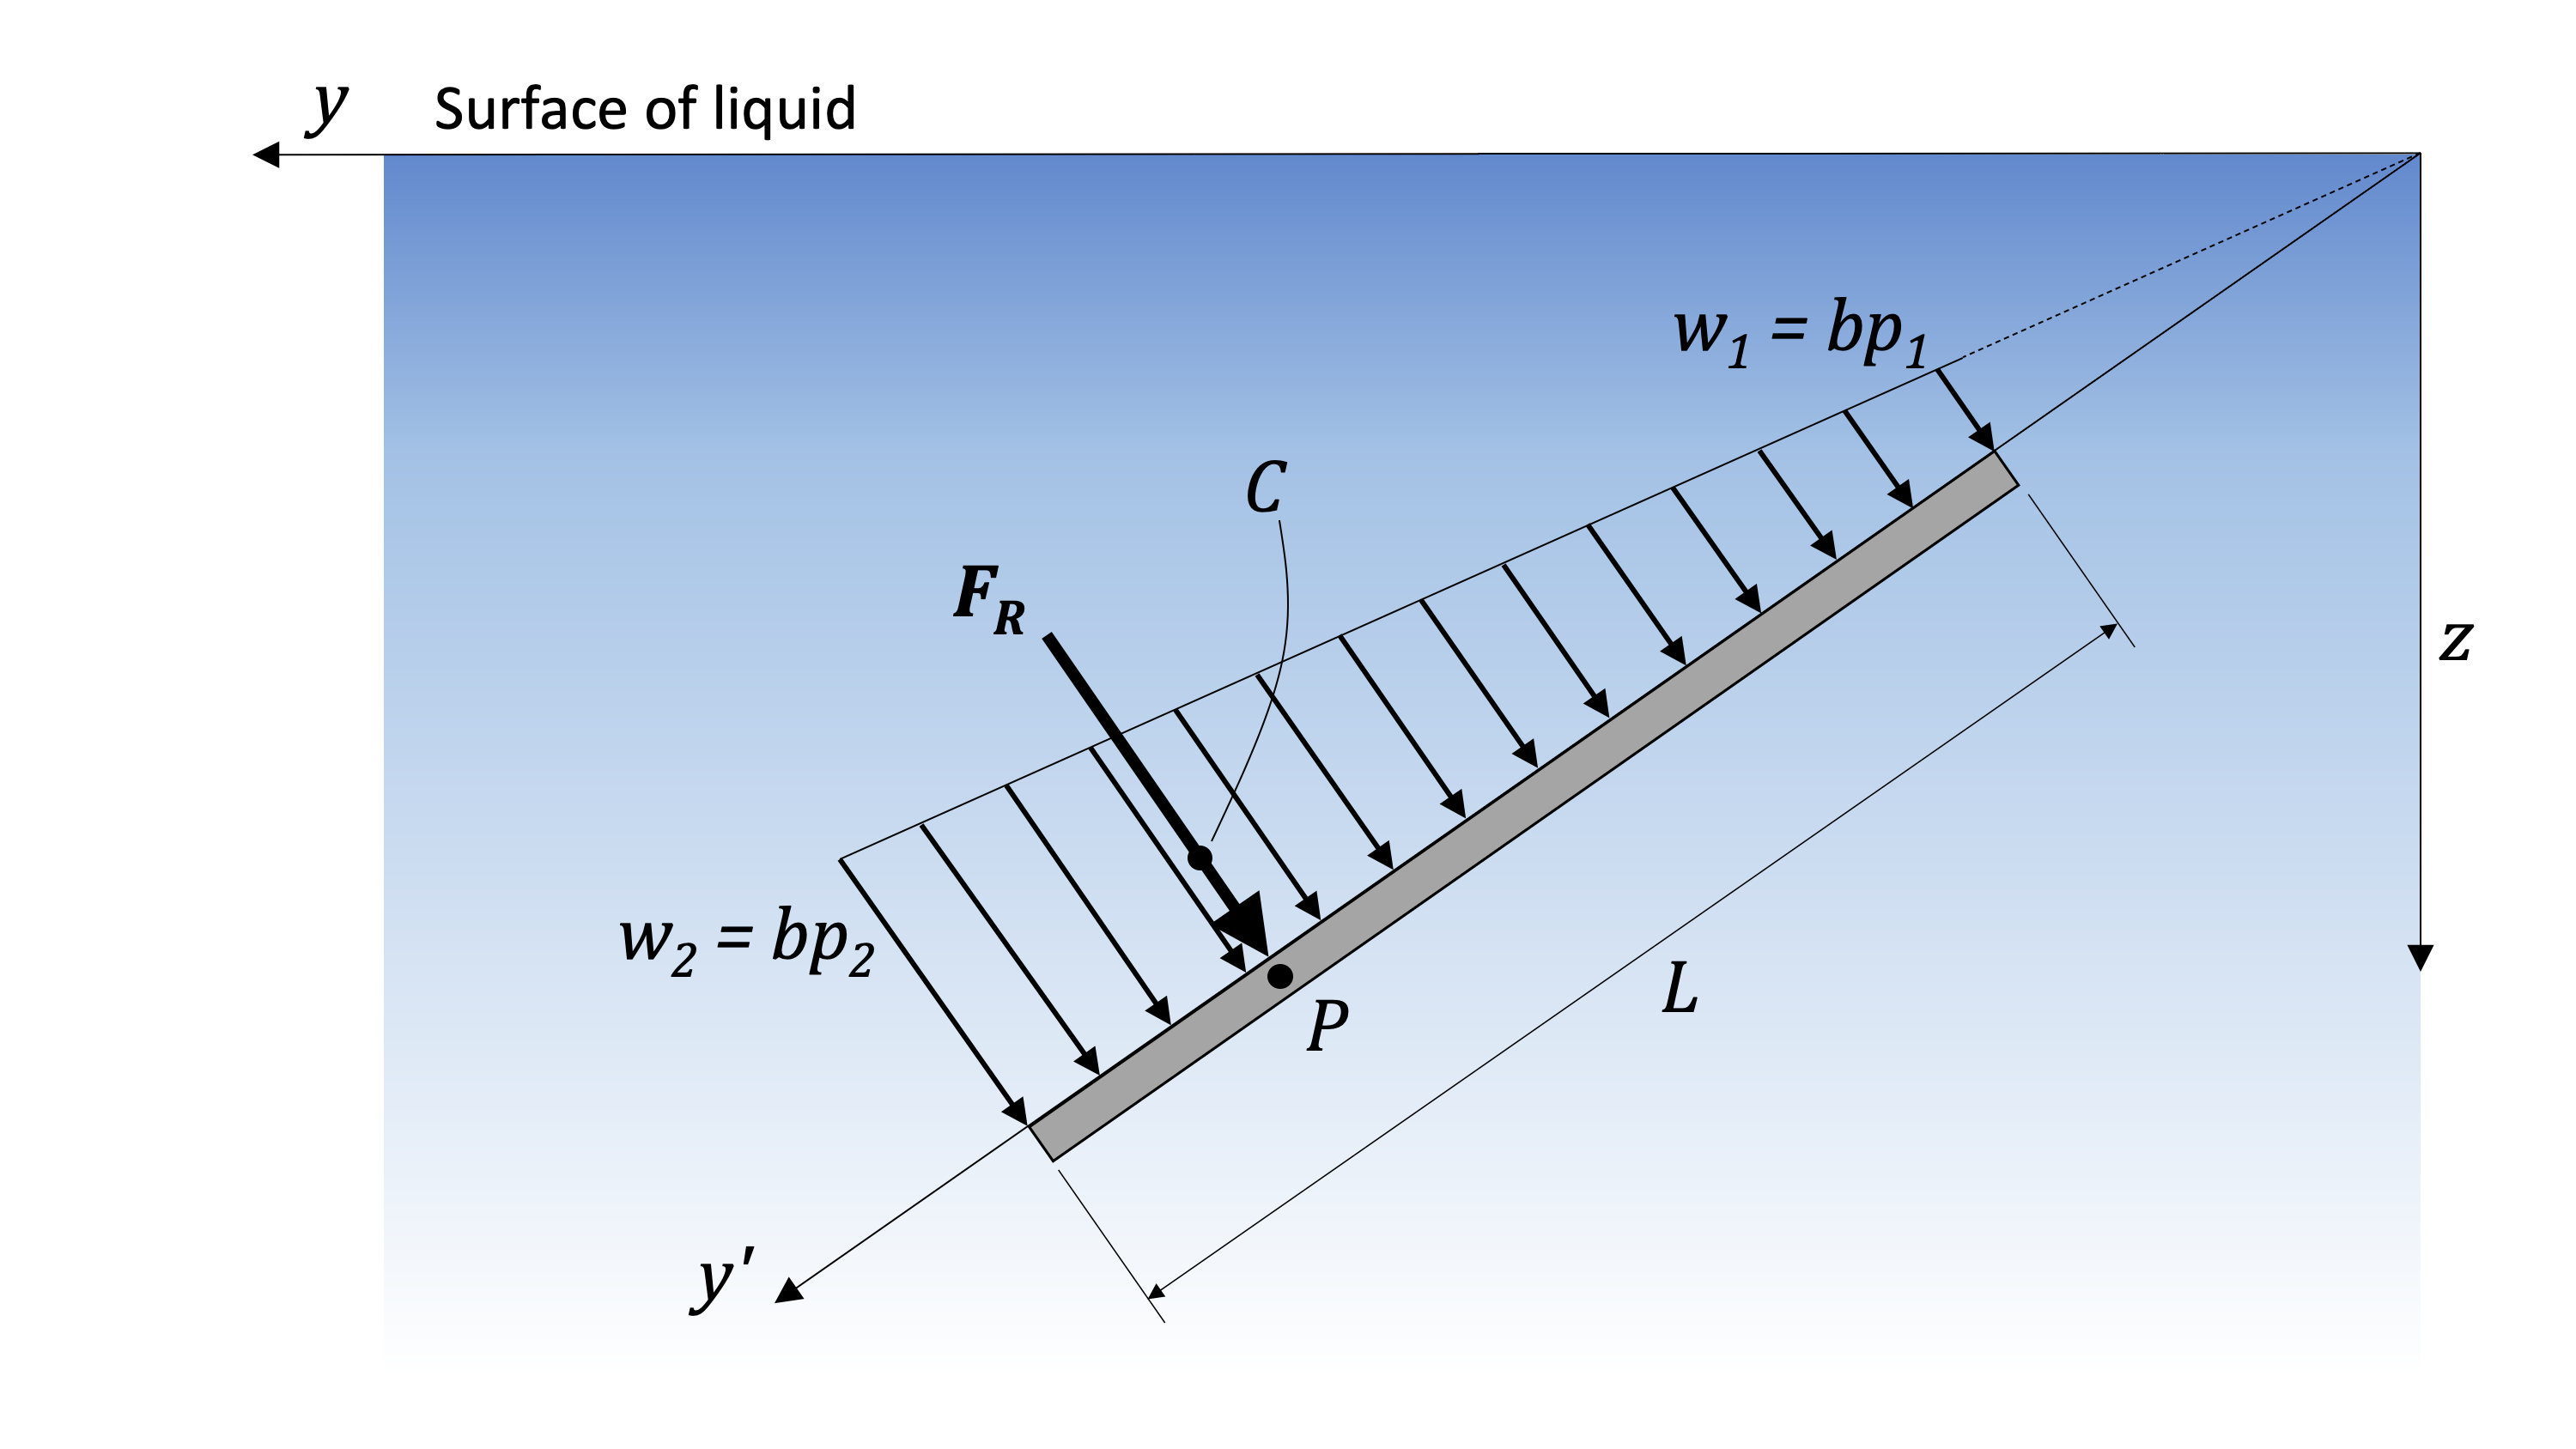
\includegraphics[trim={2cm 1cm 1cm 1cm},clip,width=0.7\textwidth, left]{Slide38} 

\vspace*{8\baselineskip}

In other words, the resultant force acts through the balance point at which there is an equal moment on each side of the point.

\subsection{Example}
Find the location of the resultant force for the pressure distribution applied to the flat plate.  

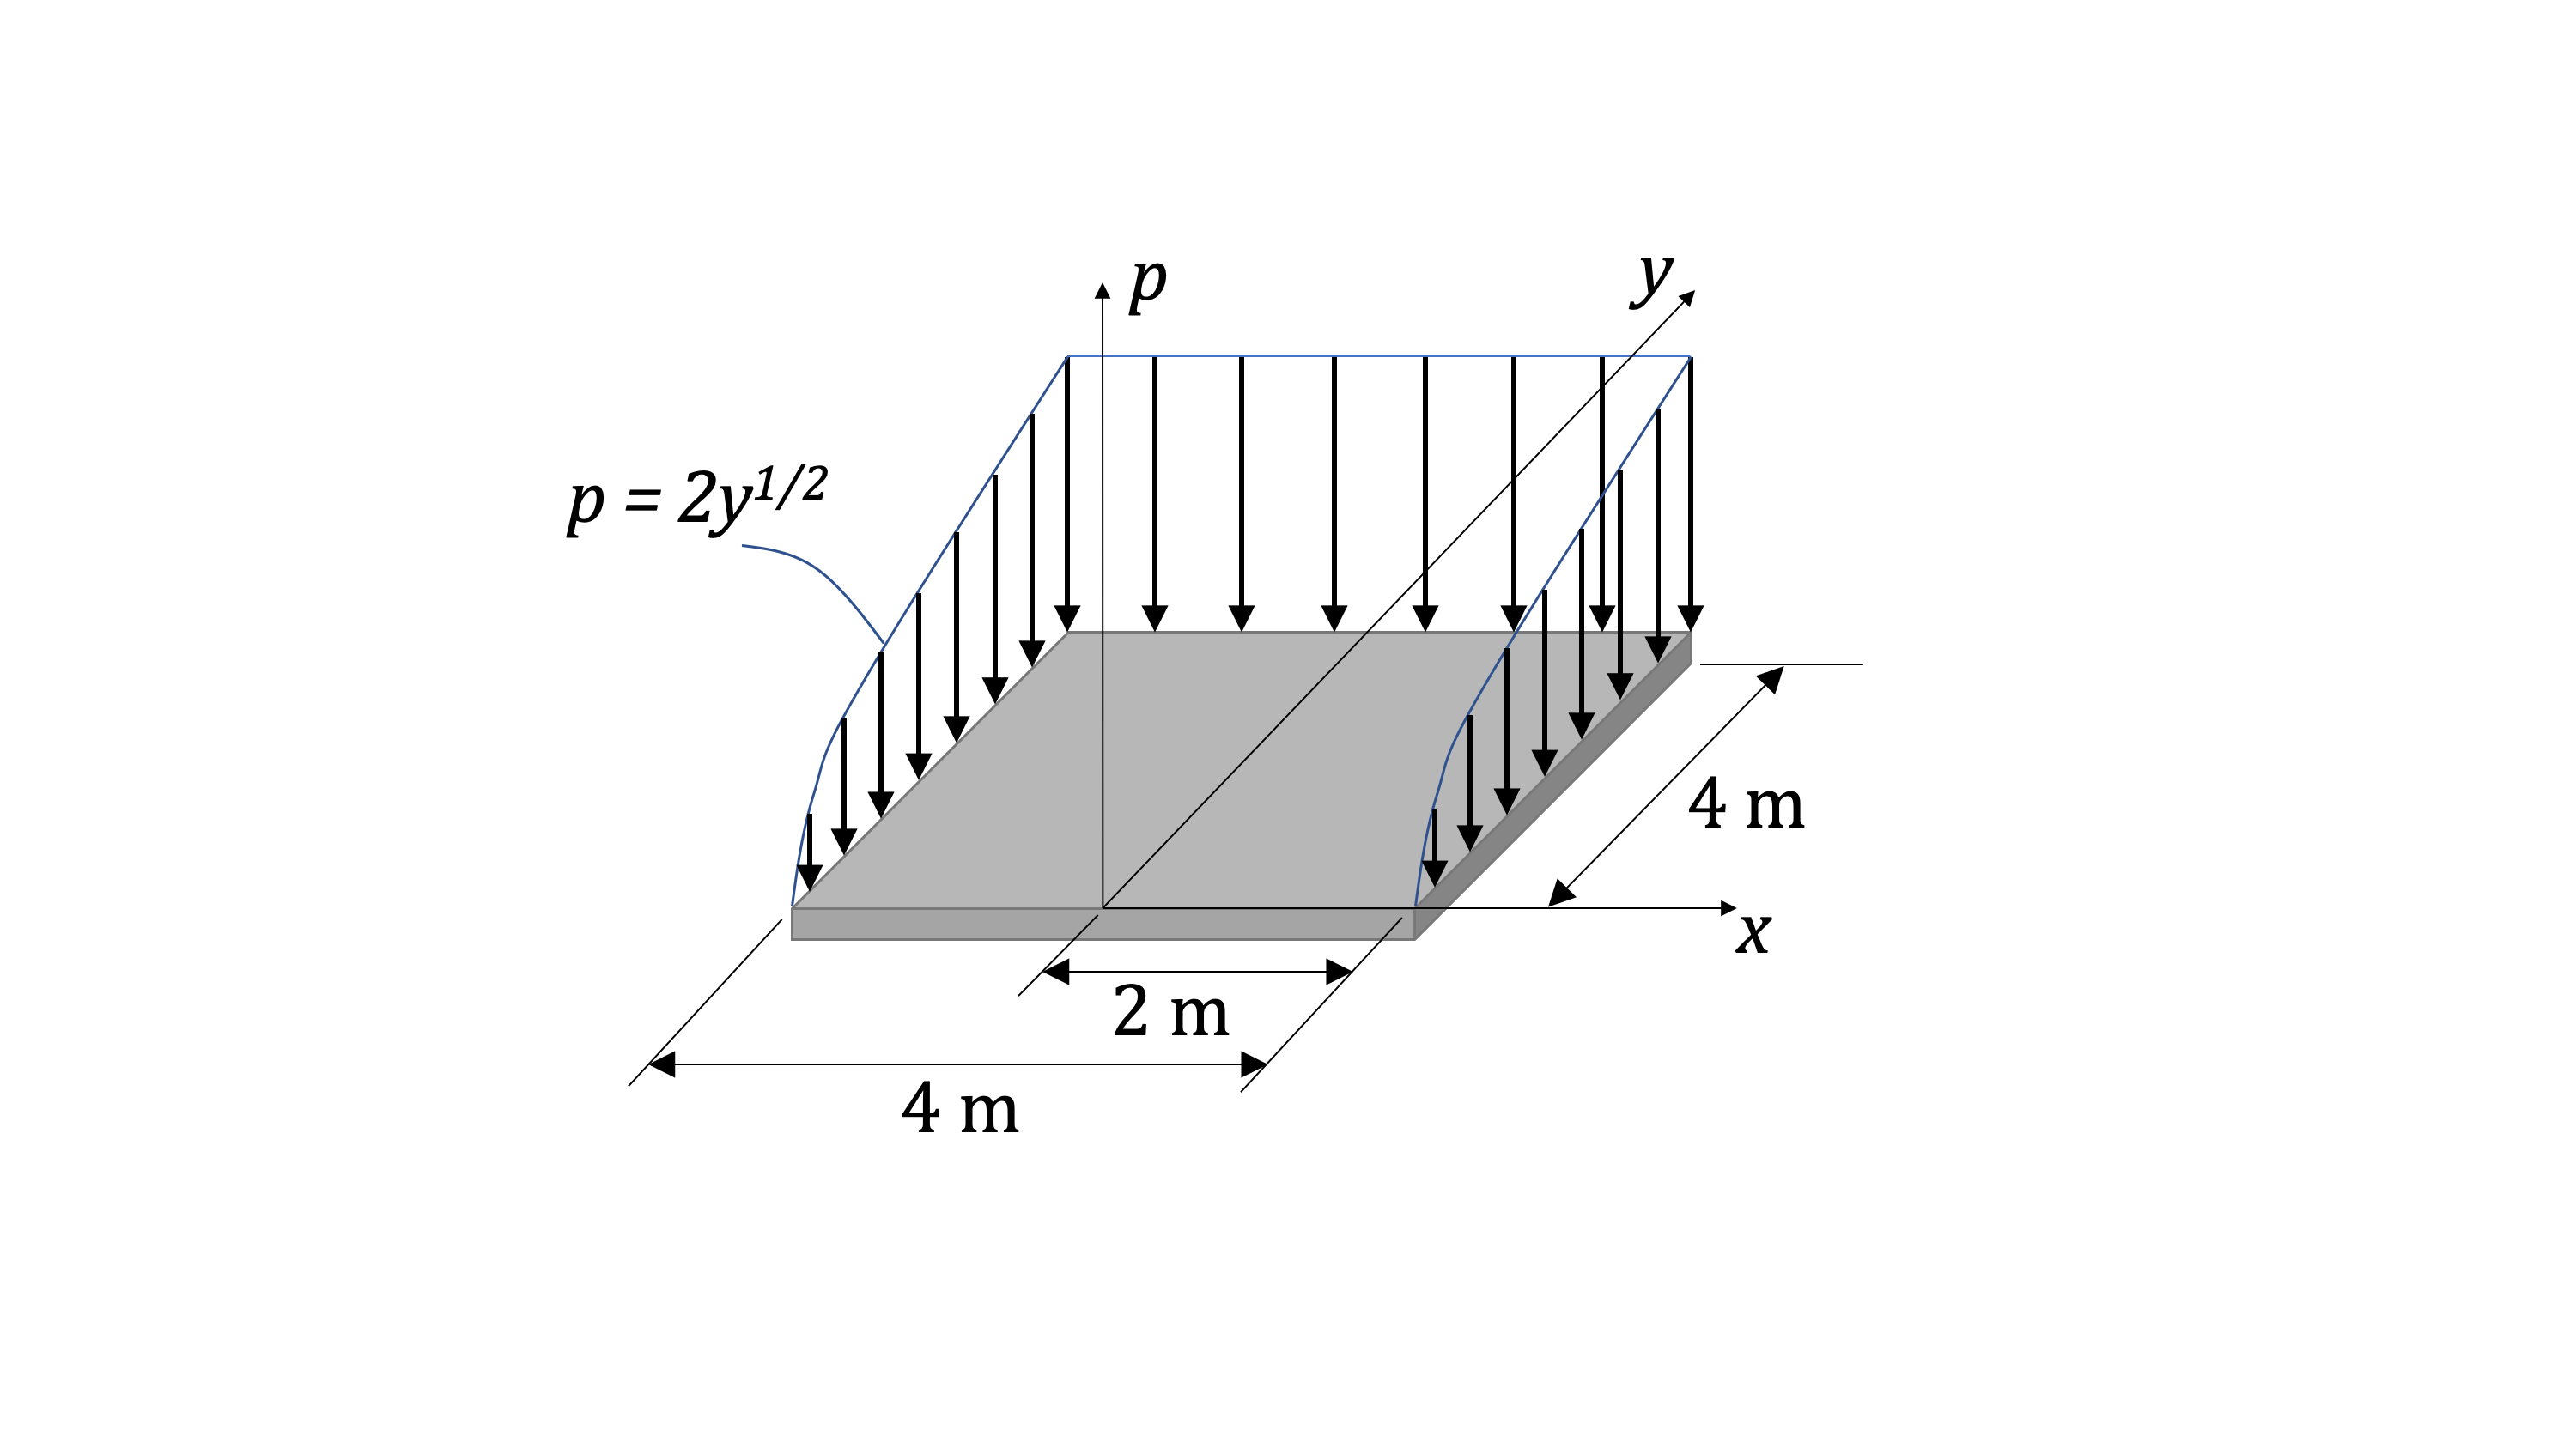
\includegraphics[trim={5cm 2cm 5cm 2cm},clip,width=0.6\textwidth, left]{Slide39} 


\vspace*{10\baselineskip}

\newpage

\section{Centre of Mass}

The centre of mass located at $\bm{r_G}=(x_G,y_G,z_G)$ is computed in a very similar manner to the centroid, where we replace $\Delta A$ or $\Delta V$ ($dA$ or $dV$) with $\Delta m$ ($dm$) as the variable of summation (integration).

\[
x_G = \frac{\displaystyle \sum_{i} x_i \Delta m_i}{\displaystyle \sum_{i} \Delta m_i} = \frac{\displaystyle \sum_{i} x_i \Delta m_i}{m} \hspace{1cm} y_G = \frac{\displaystyle \sum_{i} y_i \Delta m_i}{\displaystyle \sum_{i} \Delta m_i} = \frac{\displaystyle \sum_{i} y_i \Delta m_i}{m} 
\]

However, when computing the centre of mass, we consider that the body has a density $\rho (x,y,z)$ that could vary over the body.  For planar bodies, we will just consider $\rho (x,y)$.

Thus we have: $dm= \rho (x,y) dA = \rho (x,y) dx dy$

\vspace*{8\baselineskip}

\[
x_G = \frac{\displaystyle  \iint_m x dm }{\displaystyle  \iint_m dm} = \frac{\displaystyle \int_{x_1}^{{x_2}} \int_{y_1(t)}^{{y_2(t)}} x \rho(x) dx dy}{\displaystyle \int_{x_1}^{{x_2}} \int_{y_1(t)}^{{y_2(t)}} \rho(x) dx dy}
\]

If $\rho = constant$, then it can be cancelled out from the top and bottom of the above equation and centre of mass is the same as the centroid, $x_G=x_C$. 

Similarly $\displaystyle y_G = \frac{ \iint_m y dm }{m}$ and, for 3D bodies, $\displaystyle z_G = \frac{ \iiint_m z dm }{m}$. 

In general, $\displaystyle \bm{r_G} = \frac{\iiint_m \bm{r} dm }{m}$. 

In statics and dynamics, we resolve forces and moments applied to a body down to a \textbf{resultant force acting at the center of mass, and a resultant moment}.  

\newpage

\subsection{Example}

Find the centre of mass of a plate with density distribution $\rho = \nu x$. 

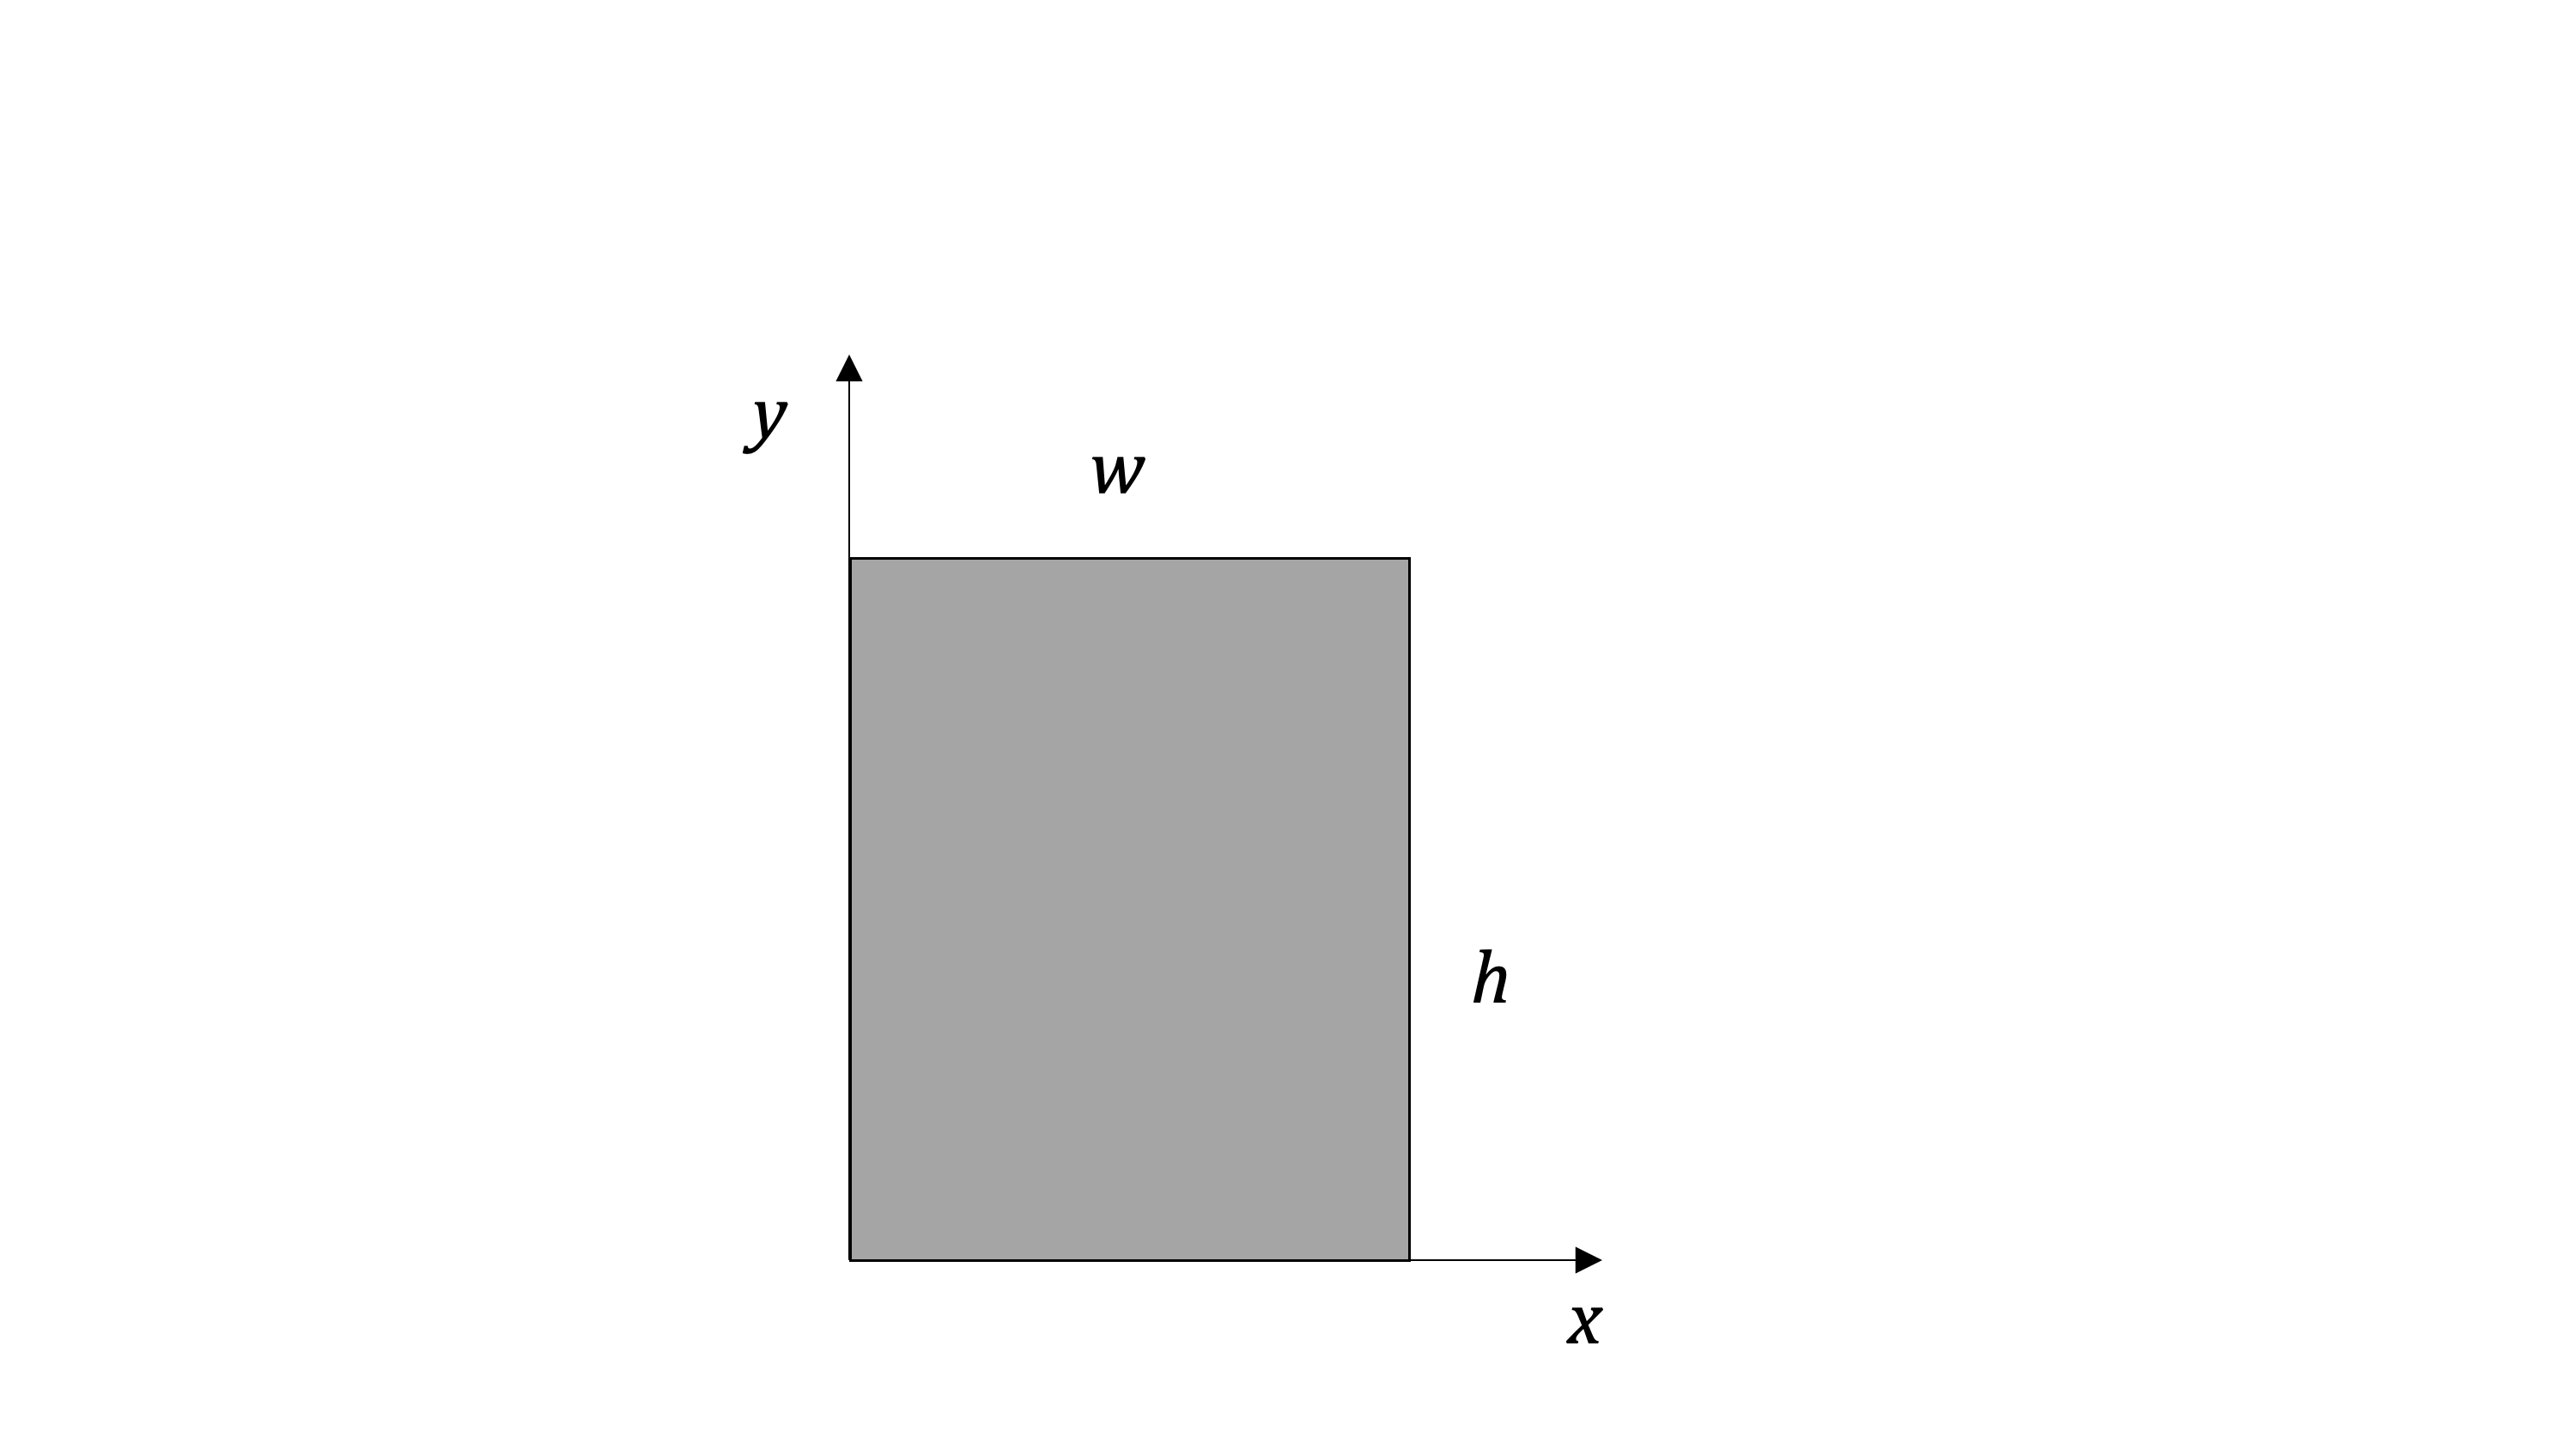
\includegraphics[trim={8cm 1cm 5cm 4cm},clip,width=0.4\textwidth, left]{Slide40} 

\vspace*{20\baselineskip}

\newpage

\section{Moments of Inertia – Second Moment of Area}
The term “moment of inertia” for an area is commonly used by engineers, but actually incorrectly applied.  For an area, the correct term is “second moment of area”.  However, due to their similarity with integrals of \textbf{mass moments of inertia}, the term sticks. 

The second moment of area is \textbf{computed about an axis} as $\displaystyle  \iint_A x^2 dA$ (note: exponent 2 = second moment), where $x$ is measured perpendicular to the axis.  

One considers the second moment of area when relating the normal stress, $\sigma$, acting on the cross-section of a beam related to an applied external moment $\bm{M}$.  

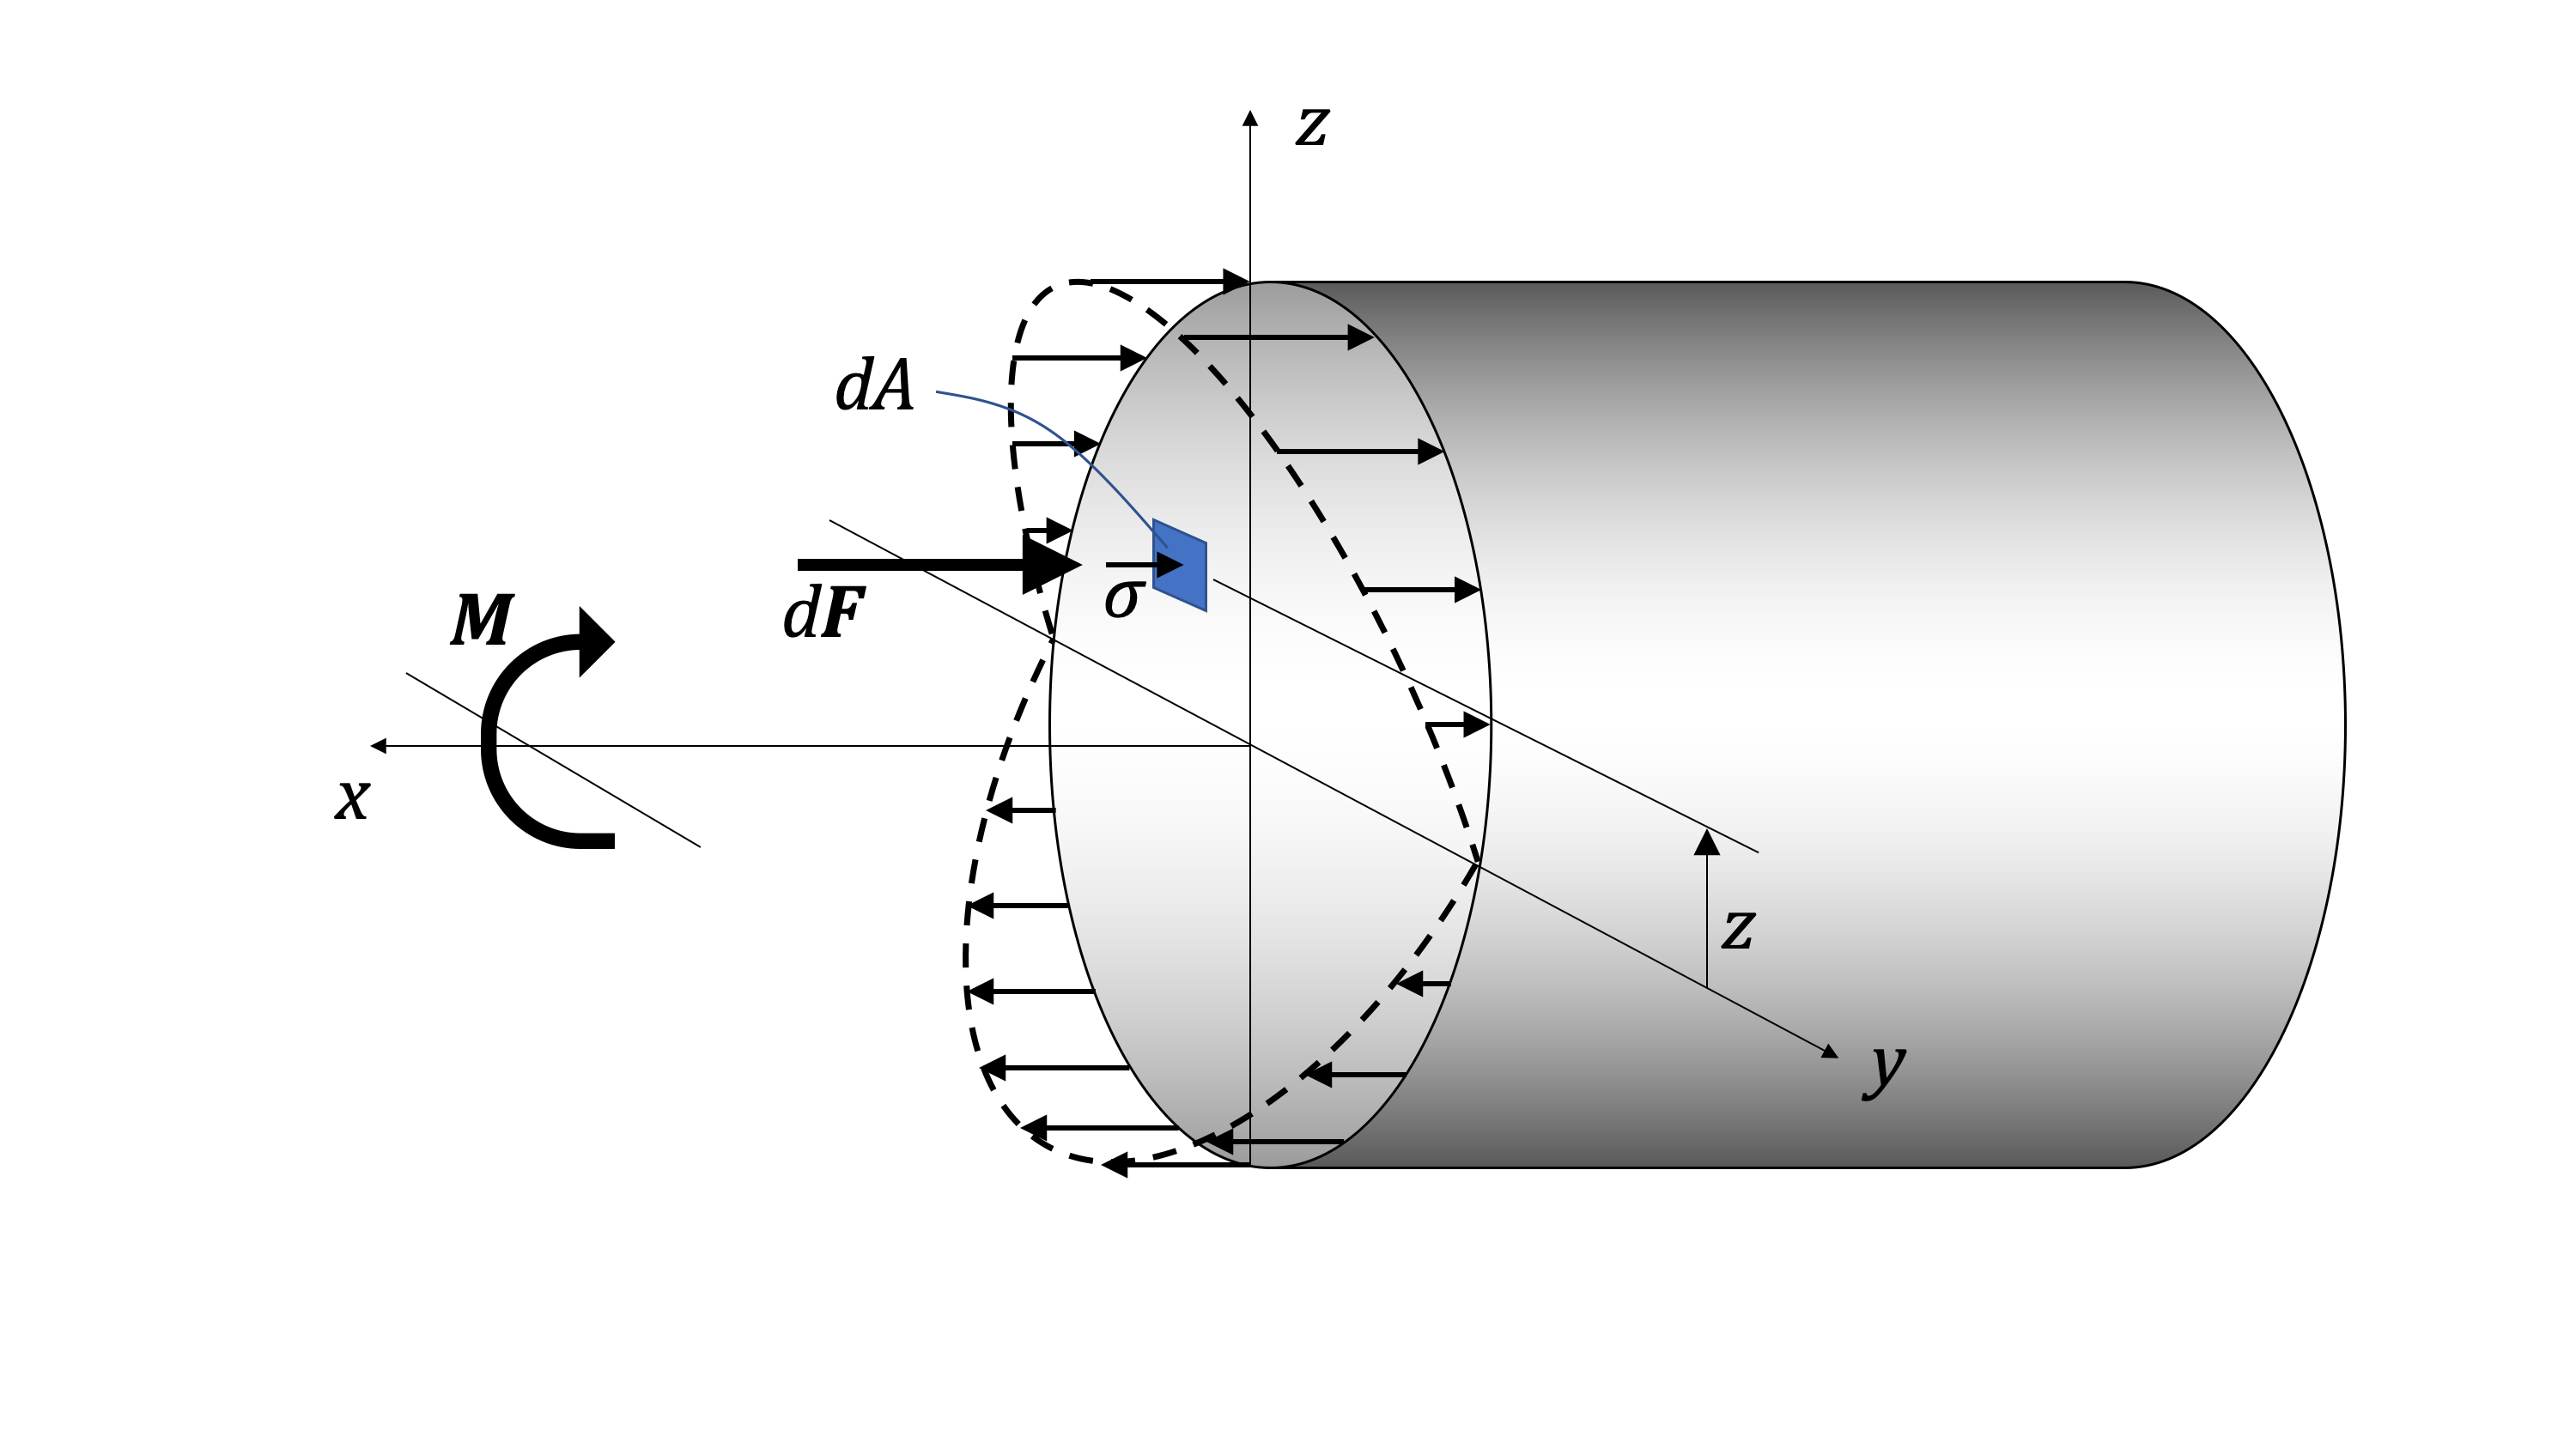
\includegraphics[trim={2.5cm 1cm 1cm 1cm},clip,width=0.6\textwidth, left]{Slide41} 

Under bending, the stress, $\sigma$, varies linearly with distance from the centroidal axis, $y$, as $\displaystyle \sigma_x = - \frac{z}{c} \sigma_m$. 

The moment (torque), $M$, about the $y$-axis is 
\[
\displaystyle M = \int -z dF = \int -z (- \frac{z}{c} \sigma_m) dA
\]  

Thus: 
\[
\displaystyle M = \frac{\sigma_m}{c} \int z^2 dA = \frac{\sigma_m}{c} I_y
\]

Rearranging, and using our first equation we get: $\displaystyle \sigma_m = - \frac{M z}{I_y}$

The second moment of area shows up in mechanics of materials, fluid mechanics, machine design, etc.

How do we find this quantity? For an area, $A$, we can compute the second moment of area around the $x$- and $y$-axes as: 

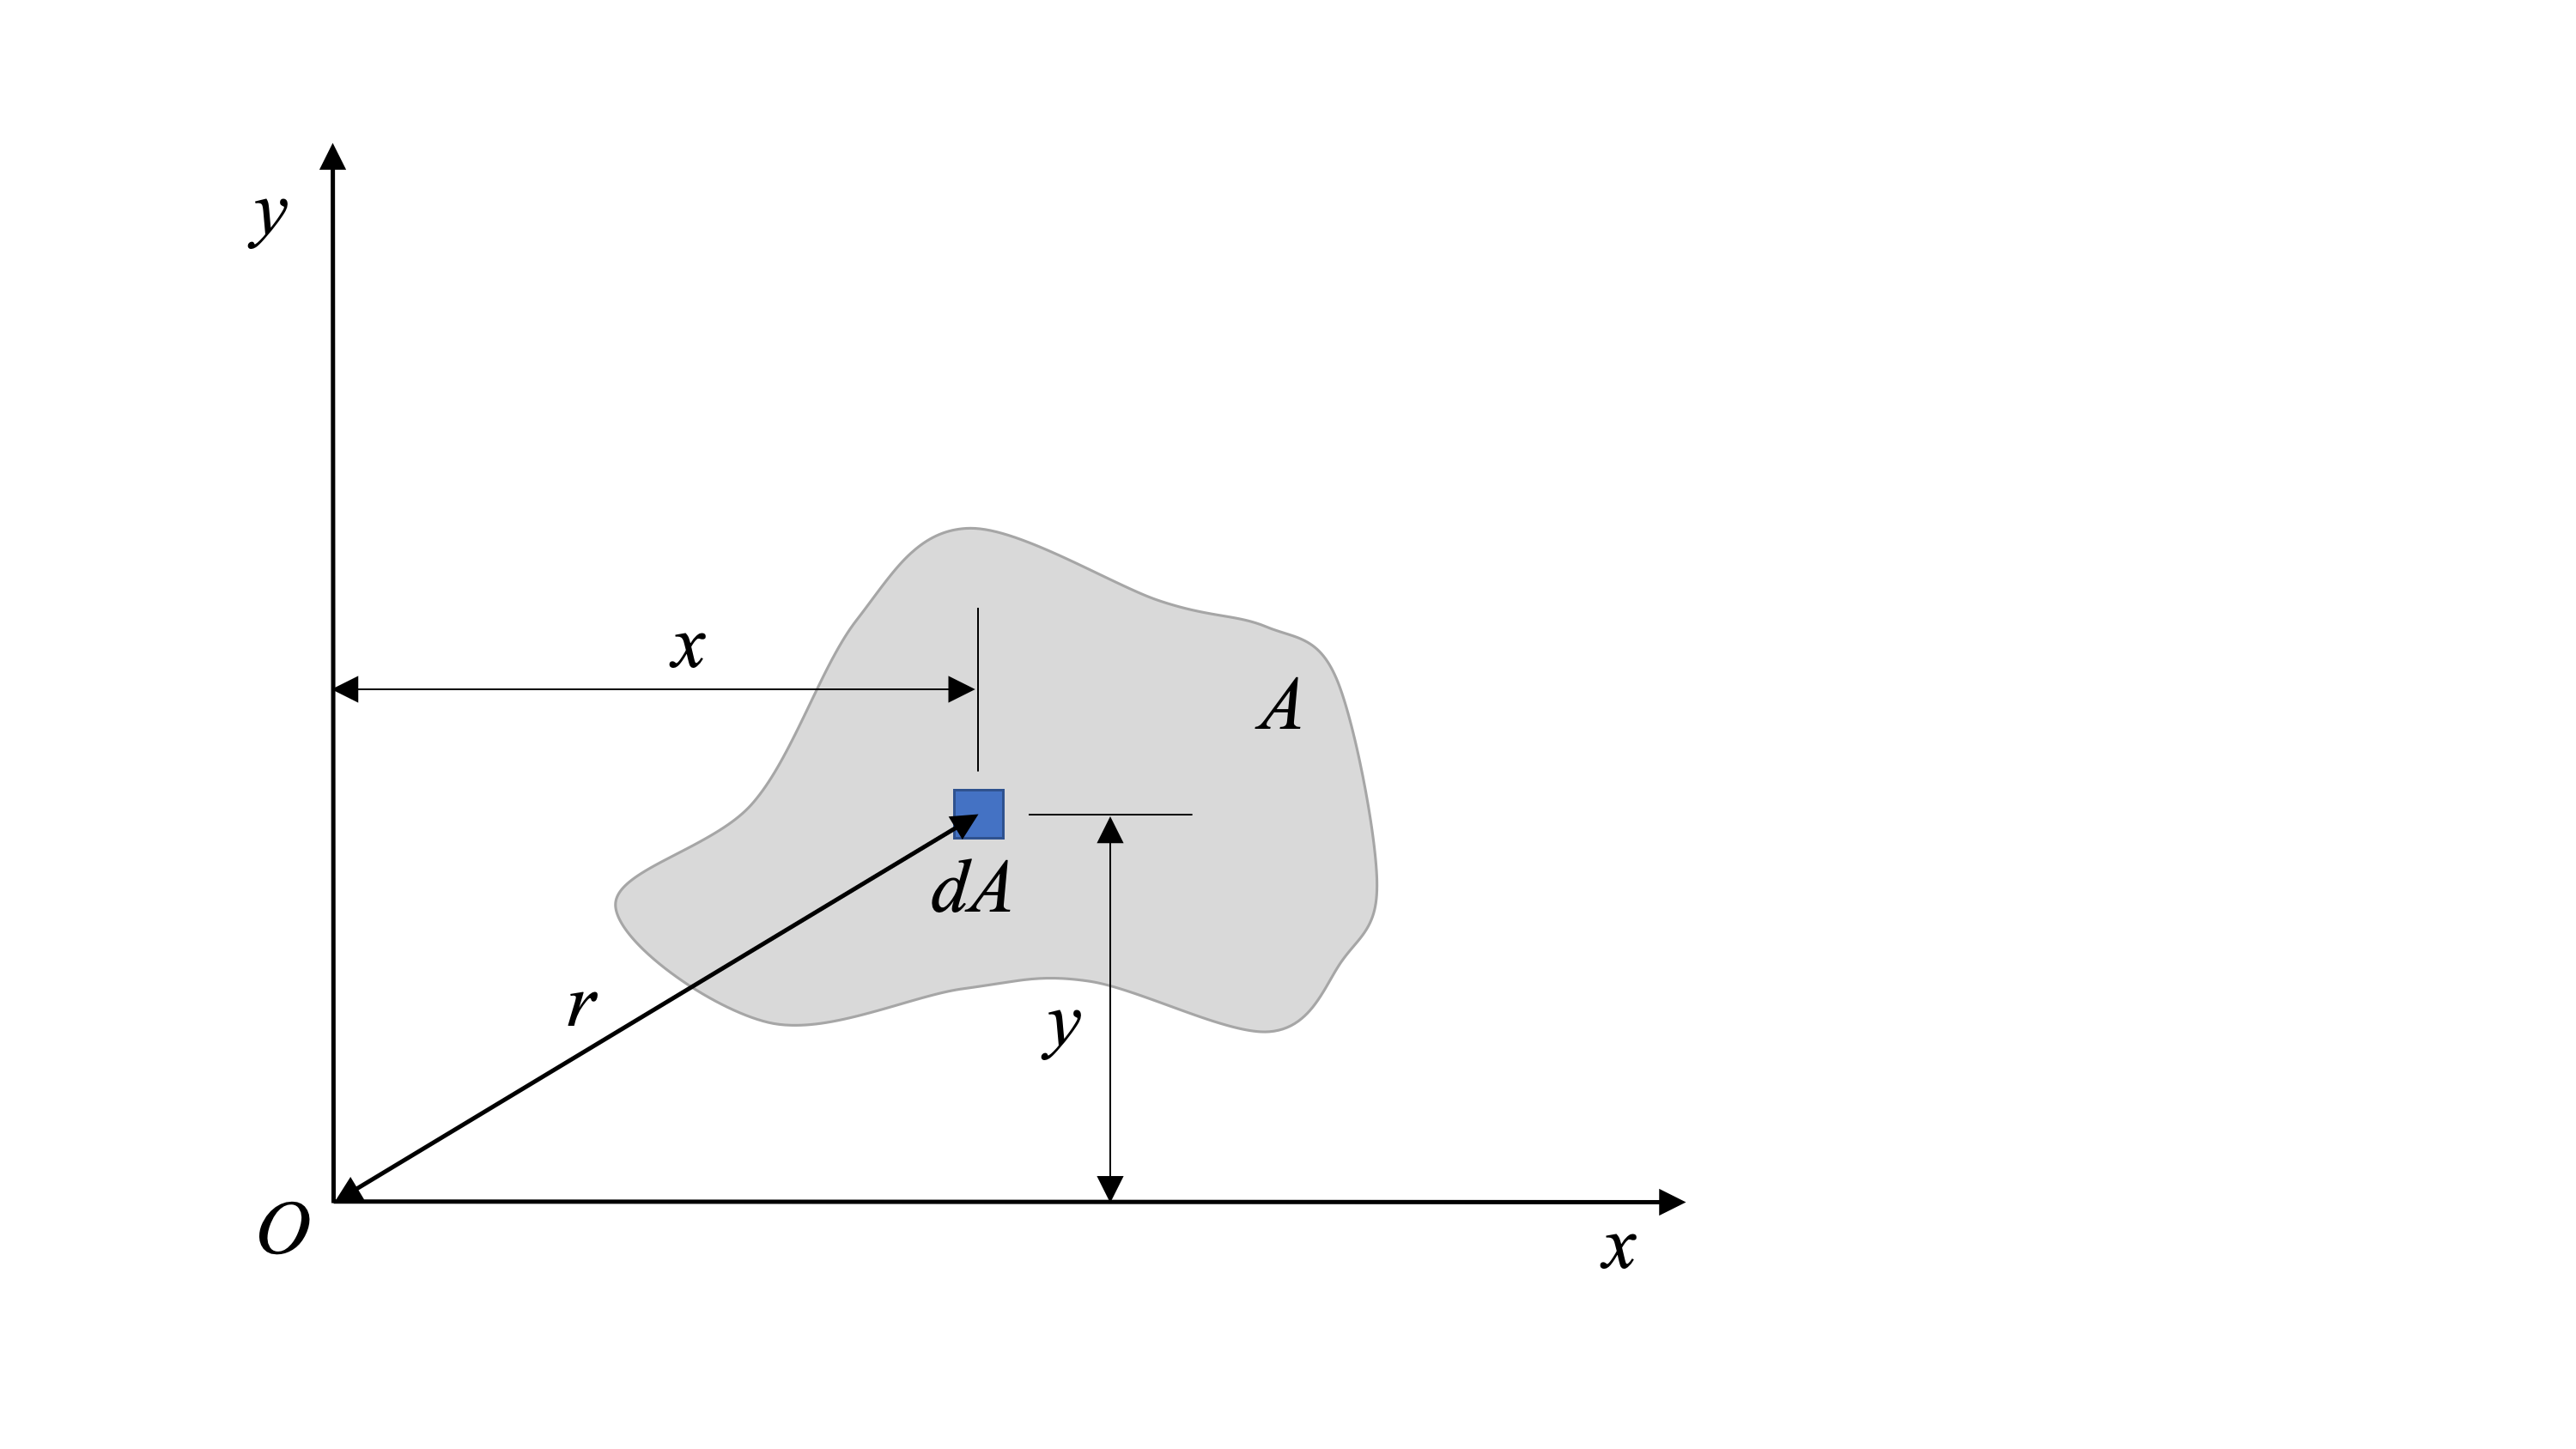
\includegraphics[trim={1cm 1cm 4cm 1cm},clip,width=0.6\textwidth, left]{Slide42} 

\[
\displaystyle I_x =   \iint_A y^2 dA = \int_{y_1}^{y_2} \int_{x_1}^{x_2} y^2 dx dy = \int_{y_1}^{y_2} y^2 [x_2(y) - x_1(y)] dy
\]
\[
\displaystyle I_y =  \iint_A x^2 dA = \int_{x_1}^{x_2} \int_{y_1}^{y_2} x^2 dy dx = \int_{x_1}^{x_2} x^2 [y_2(x) - y_1(x)] dx
\]

Around the $z$ axis, we compute the second moment of area about the “pole” coming out of point $O$, and this is referred to as the \textbf{polar moment of inertia}.  
\[
\displaystyle J_O =  \iint_A \bm{r}^2 dA =  \iint_A (x^2 + y^2) dA = I_x + I_y
\]

Notes:  
\begin{itemize}
\item The value of the moment of area depends on the axis about which it is computed!  Often, these values are compute about centroidal axes (axes passing through the centroid).
\item Moments of areas about an axis can be added and subtracted to compute the moments of complex shapes

\end{itemize}

\newpage

\subsection{Example}
Find the second moment of area (moment of inertia) and polar moment of inertia of a rectangular plate about the centroidal axes parallel to the $x$, $y$, and $z$ axes shown.  

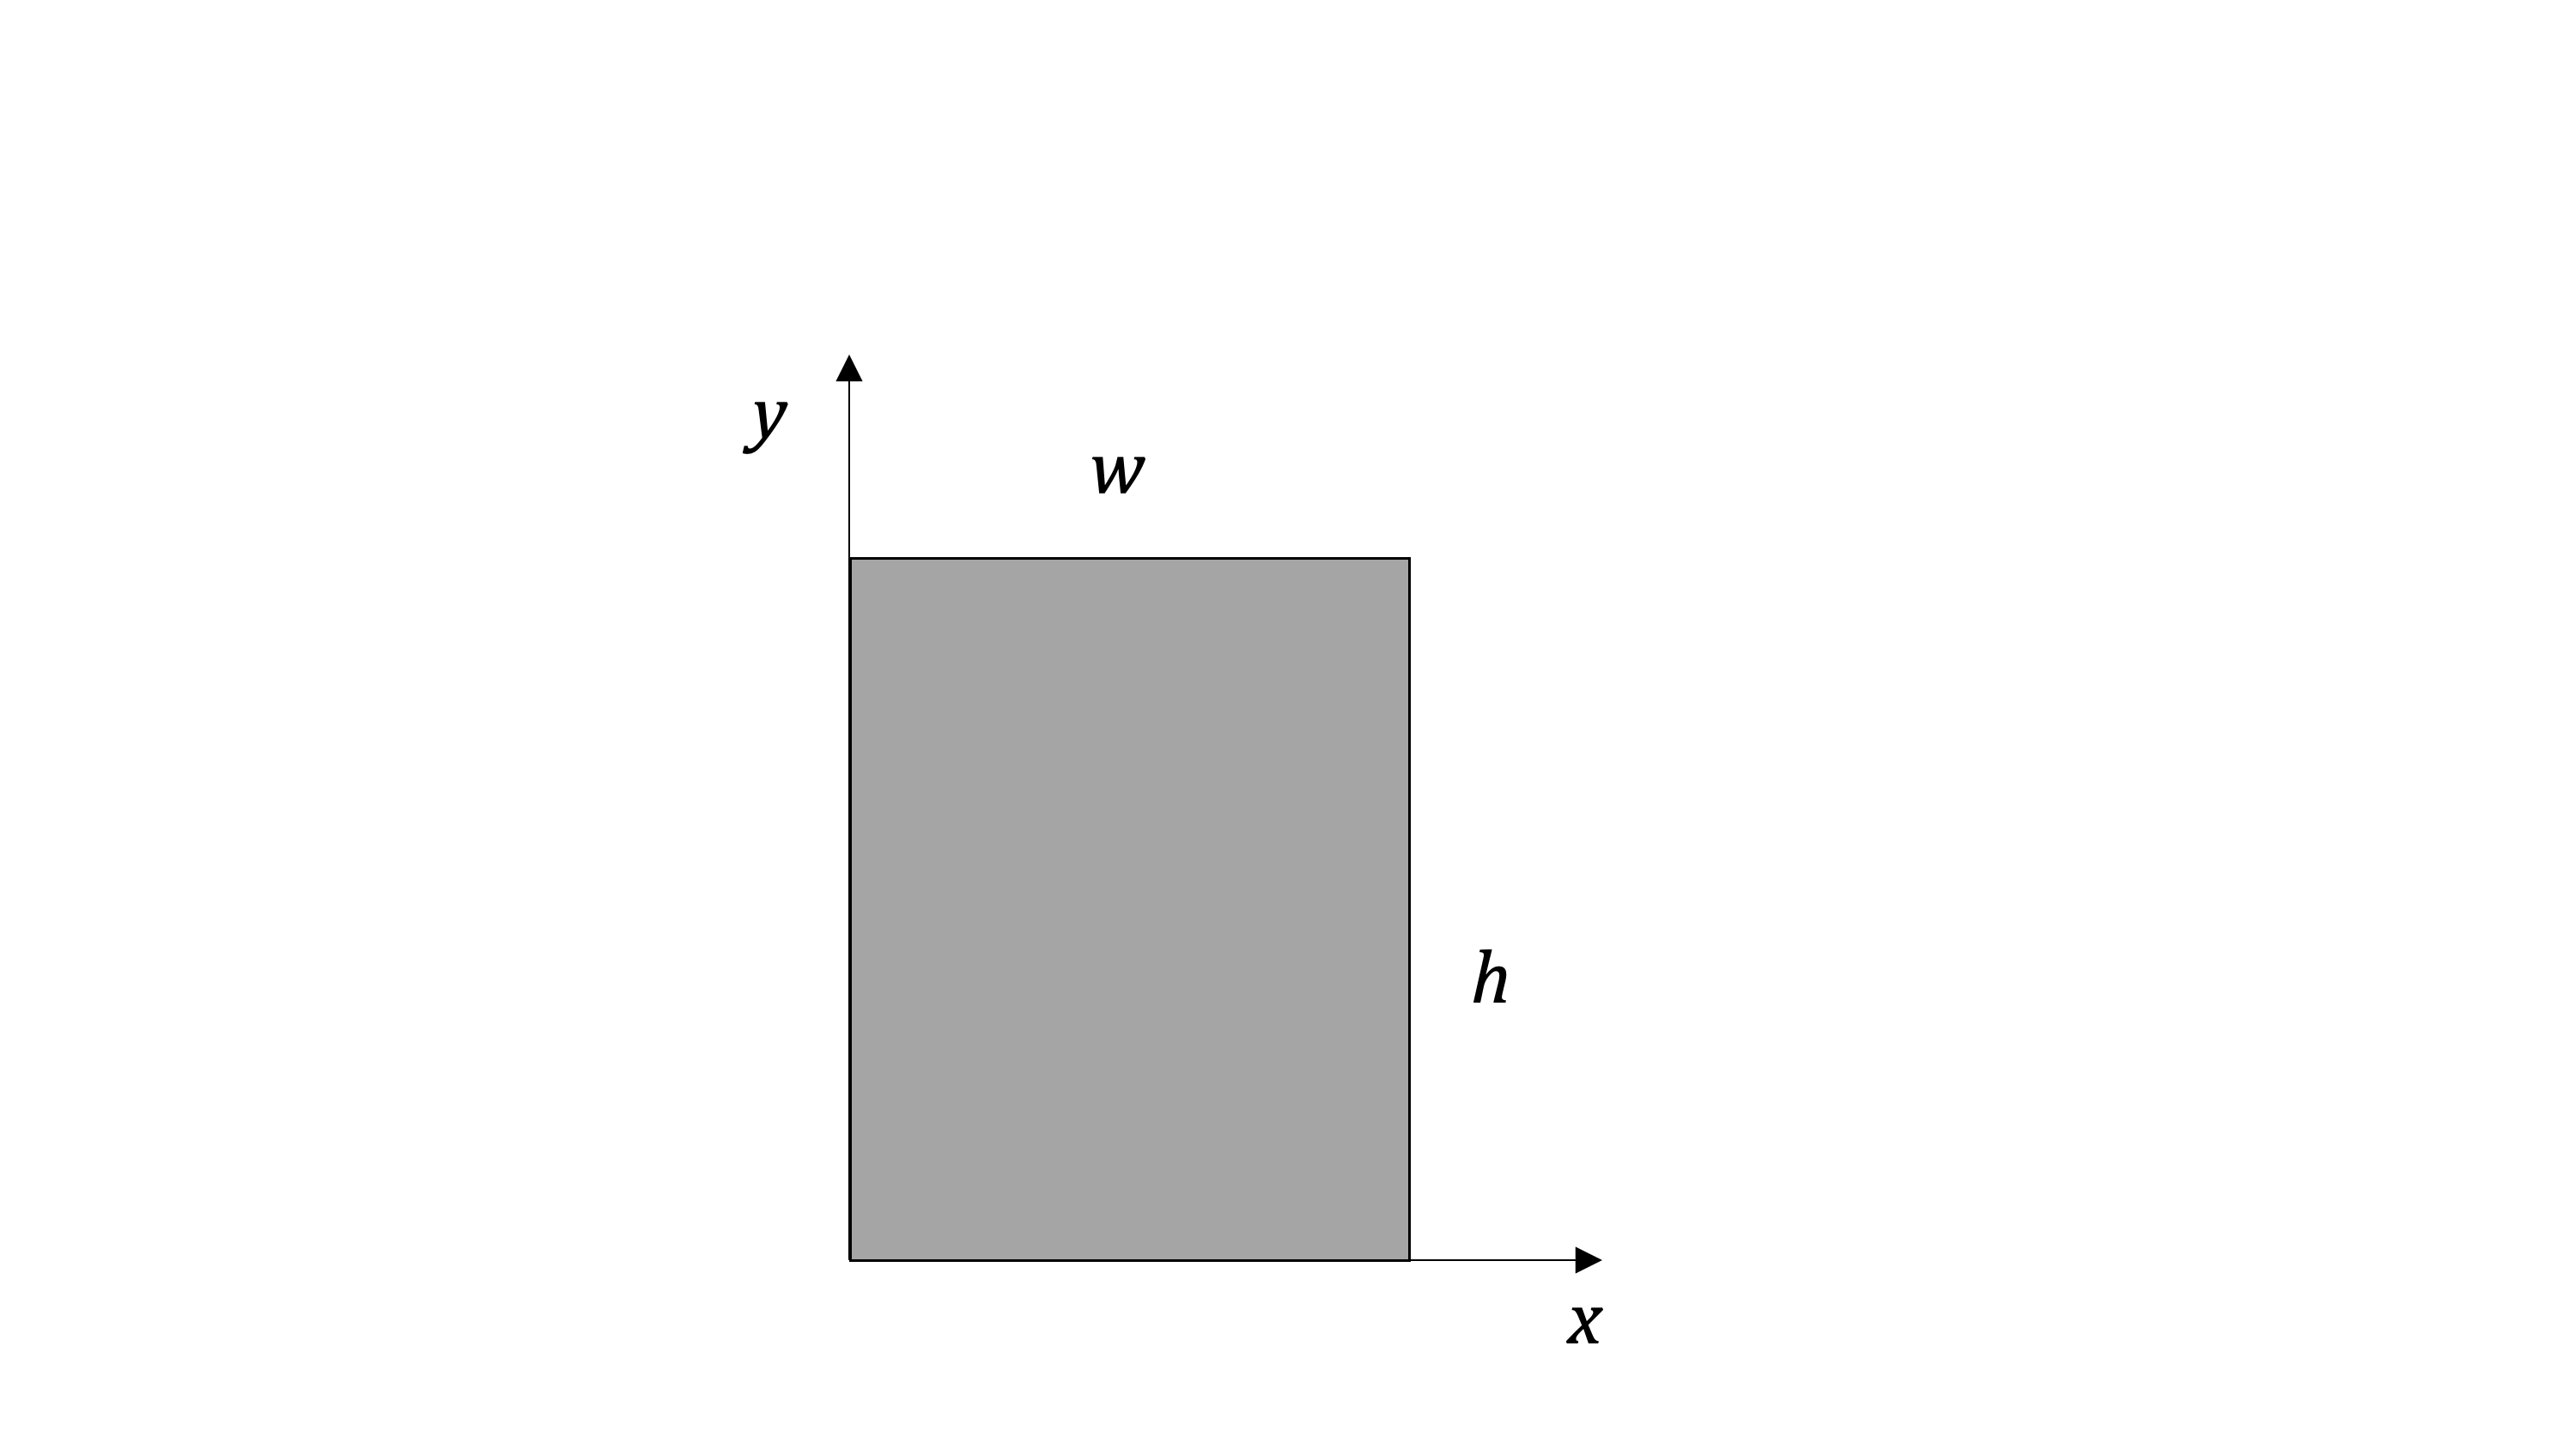
\includegraphics[trim={8cm 1cm 5cm 4cm},clip,width=0.4\textwidth, left]{Slide40} 

\vspace*{8\baselineskip}

A rectangle of height $\displaystyle \frac{h}{2}$ and width $\displaystyle \frac{w}{3}$ is cut out of the plate. Repeat the computation above.

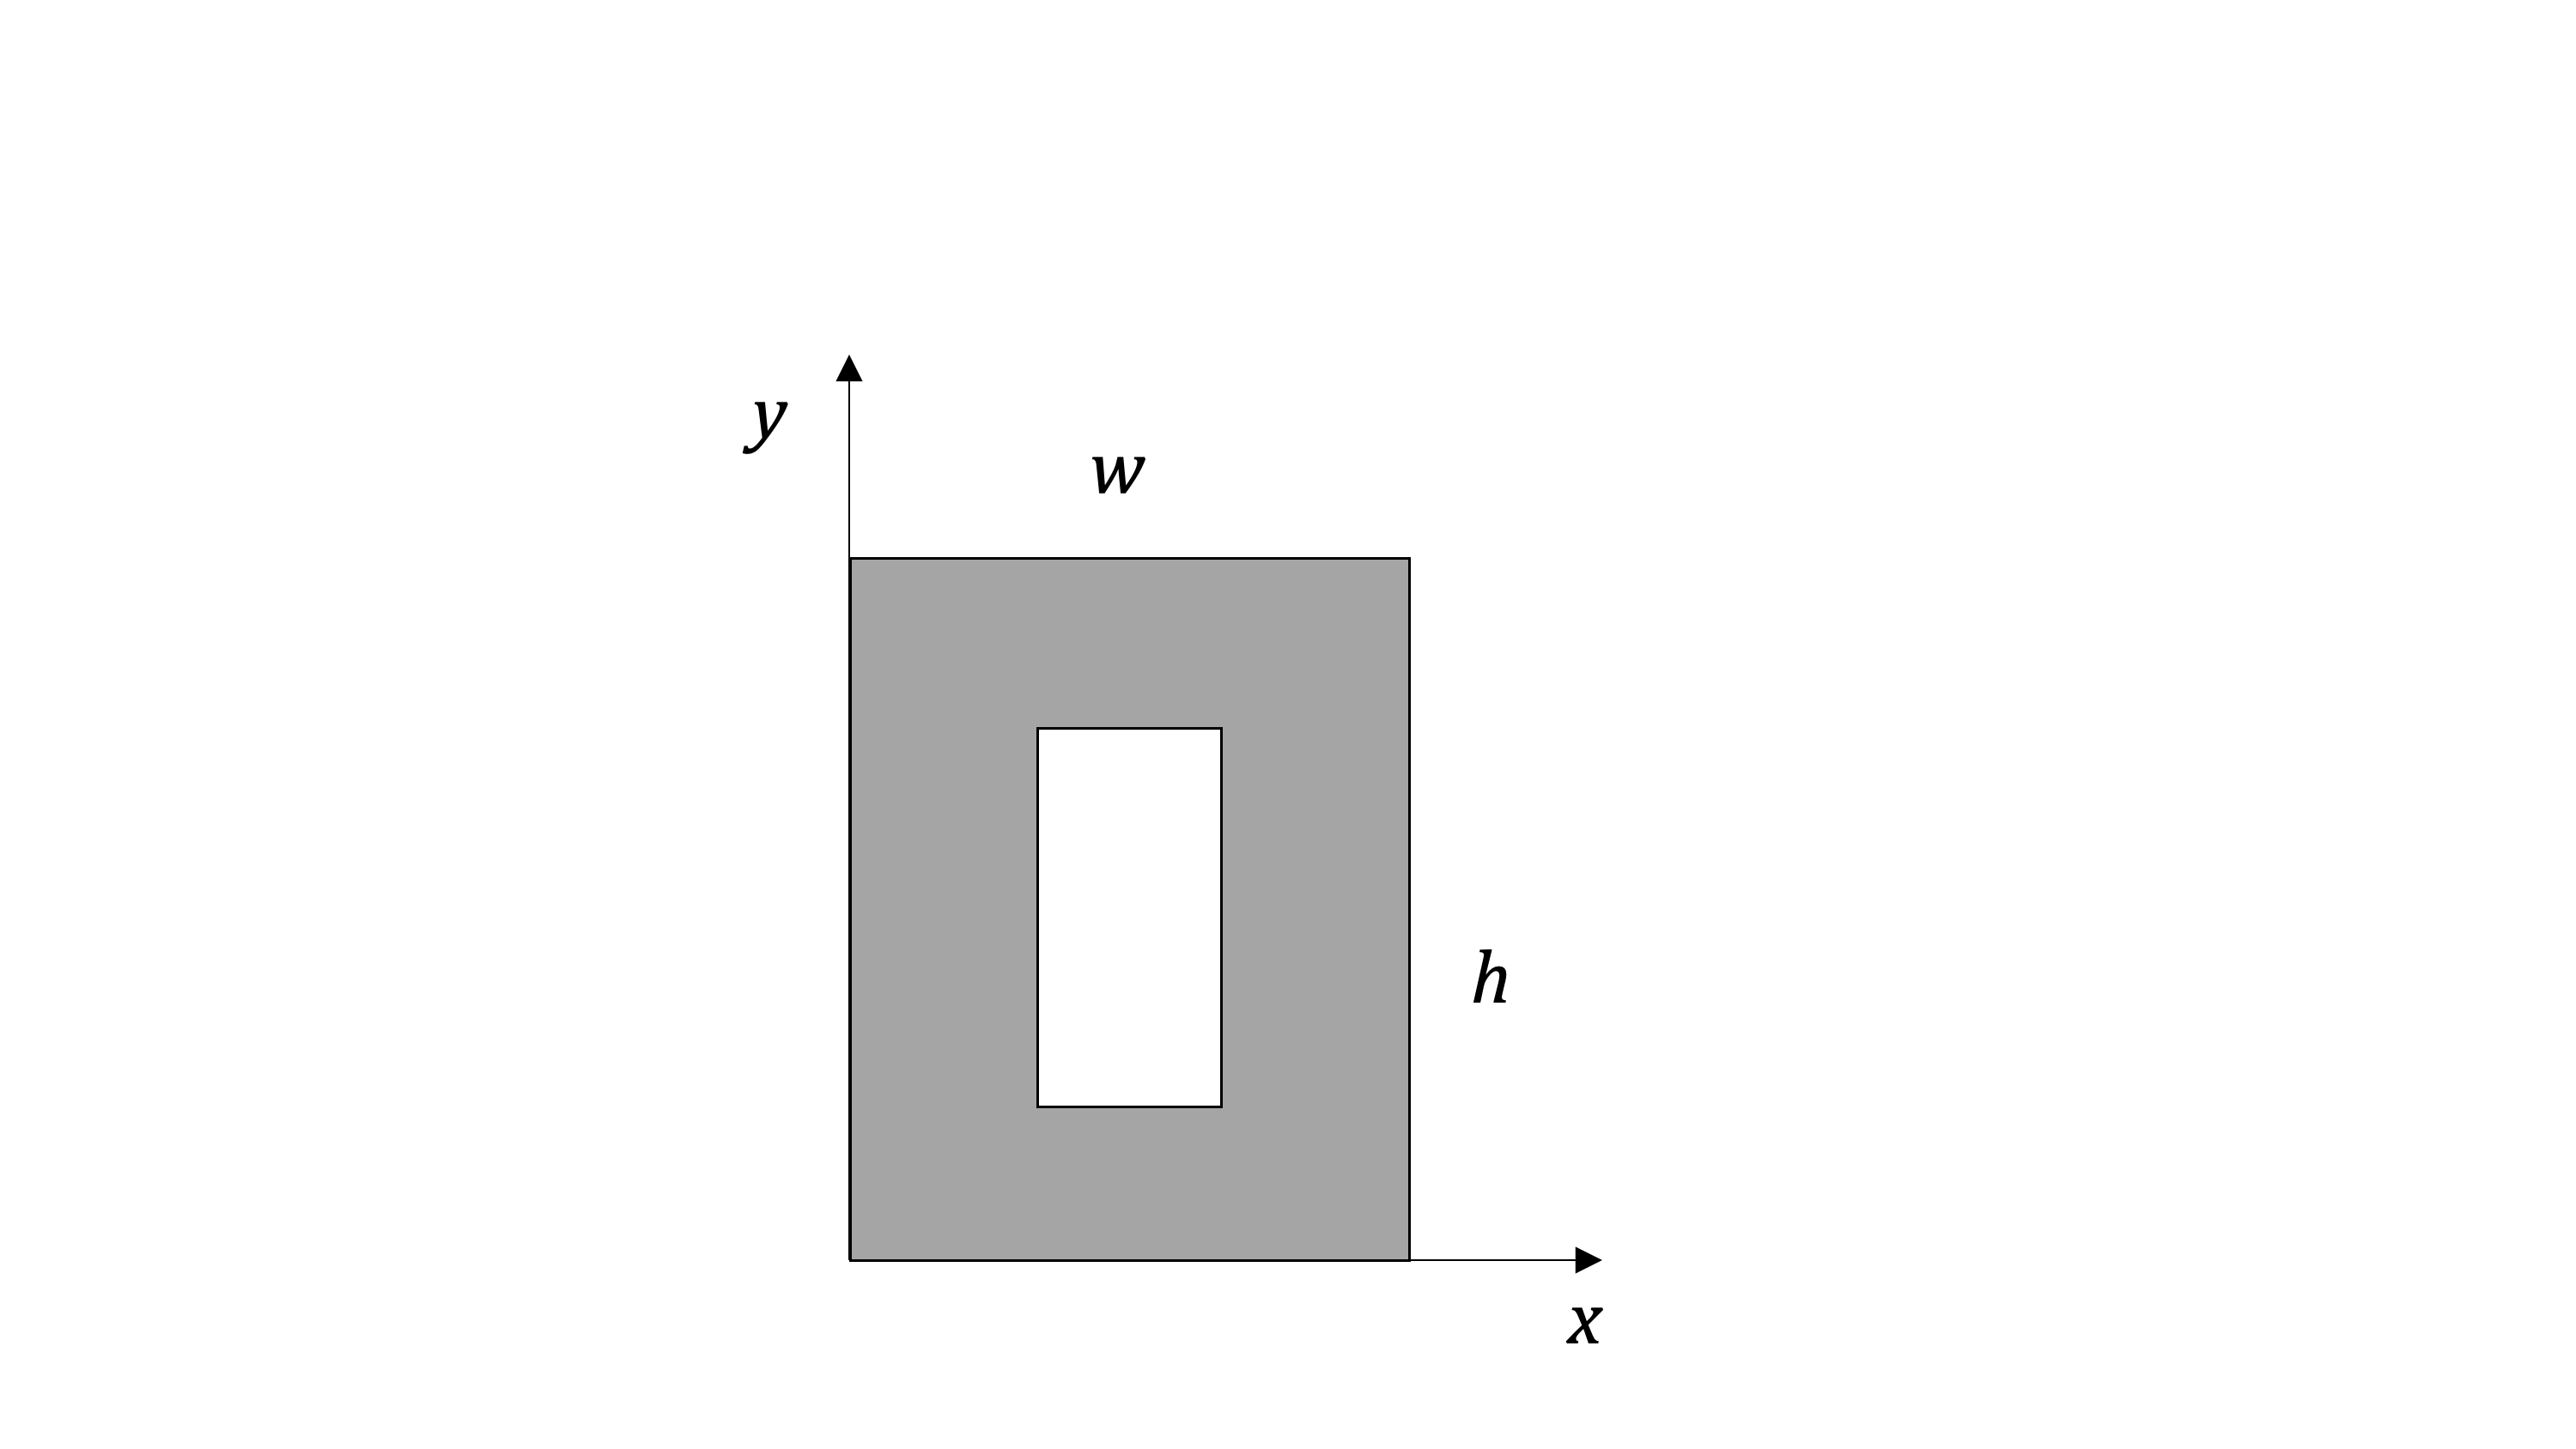
\includegraphics[trim={8cm 1cm 5cm 4cm},clip,width=0.4\textwidth, left]{Slide43} 

\newpage

\section{Mass Moment of Inertia}
The mass moment of inertia is a measure of resistance of a body to angular acceleration, the same way that mass is a measure of a body’s resistance to acceleration: 
\[ 
\bm{M} = I_G \bm{\alpha} \hspace{4 cm} \bm{F} = m \bm{a}
\]

The mass moment of inertia is the integral of the second moment about an axis of all the elements of mass, $dm$, which compose the body, $\displaystyle I =  \iint_m \bm{r}^2 dm$.

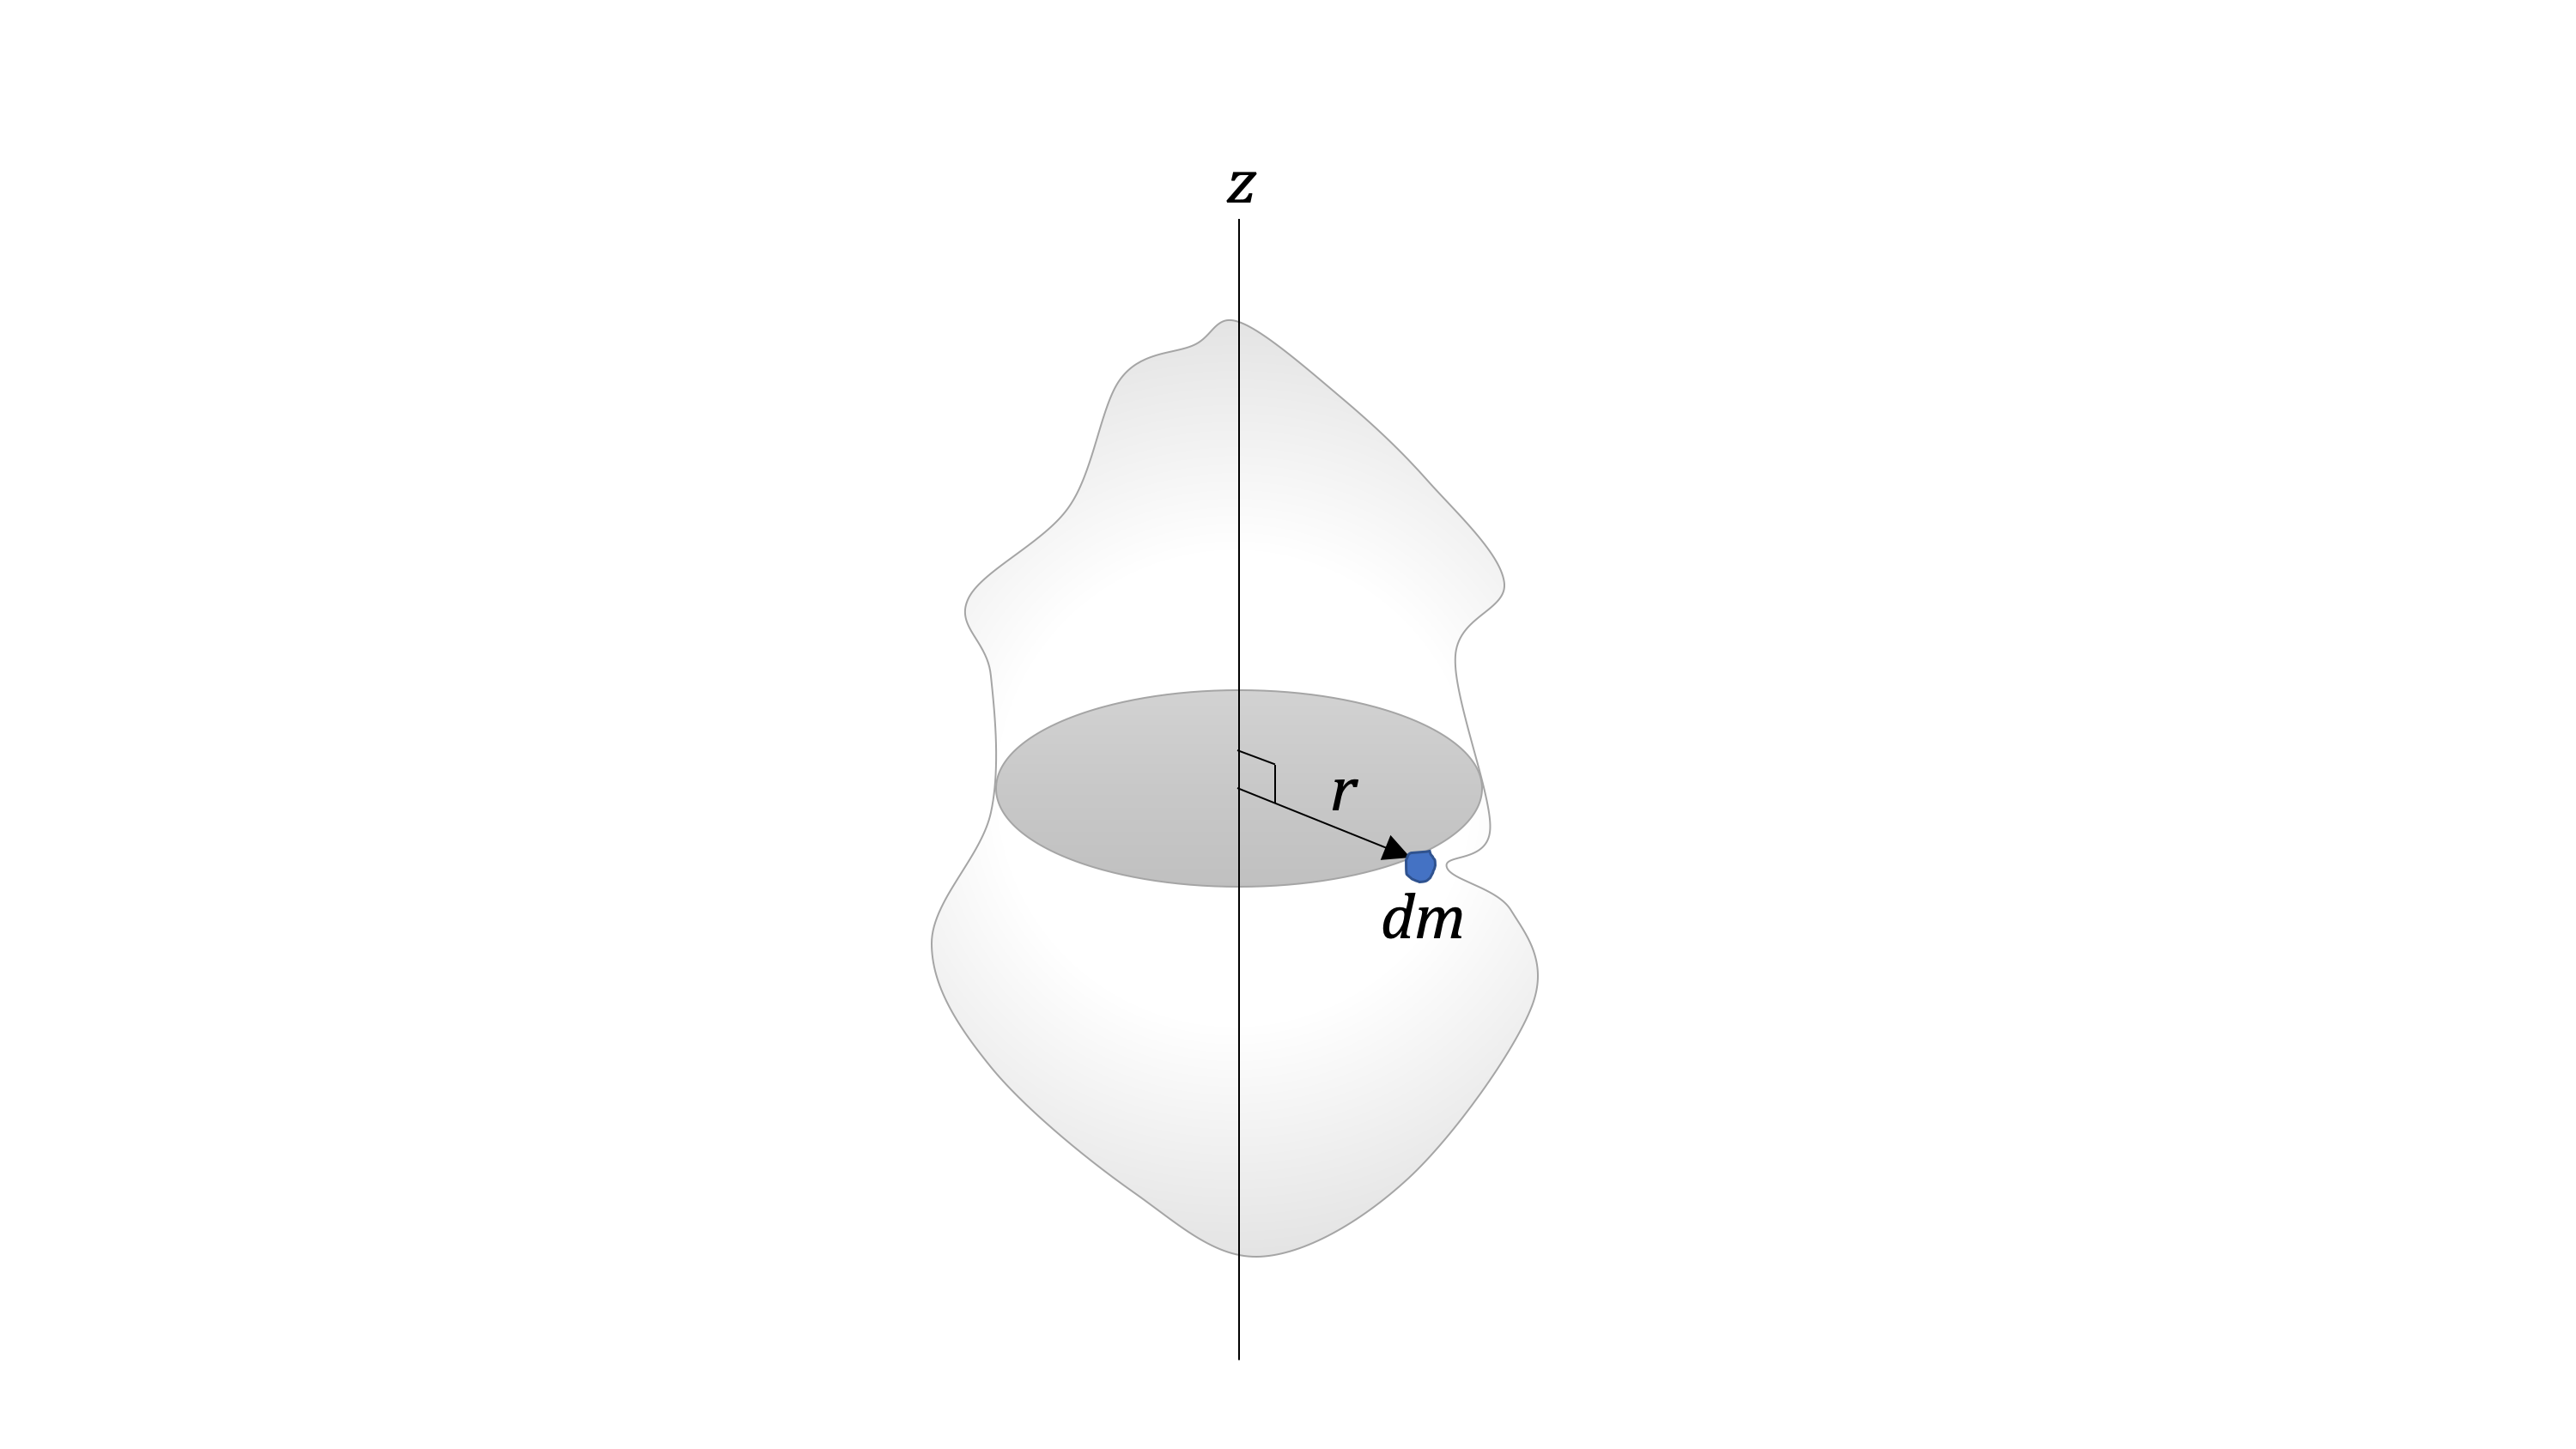
\includegraphics[trim={8cm 1cm 5cm 1.5cm},clip,width=0.4\textwidth, left]{Slide44} 

Again, we can compare this to the second moment of area if we consider a body with constant depth, $h$, and constant density, $\rho$:

\[
\displaystyle I_{zz} =  \iint_m \bm{r}^2 dm =  \iint_m \bm{r}^2 \rho h dx dy = \rho h  \iint_A (x^2 + y^2) dx dy = \rho h (I_x + I_y) = \rho h J_O
\]

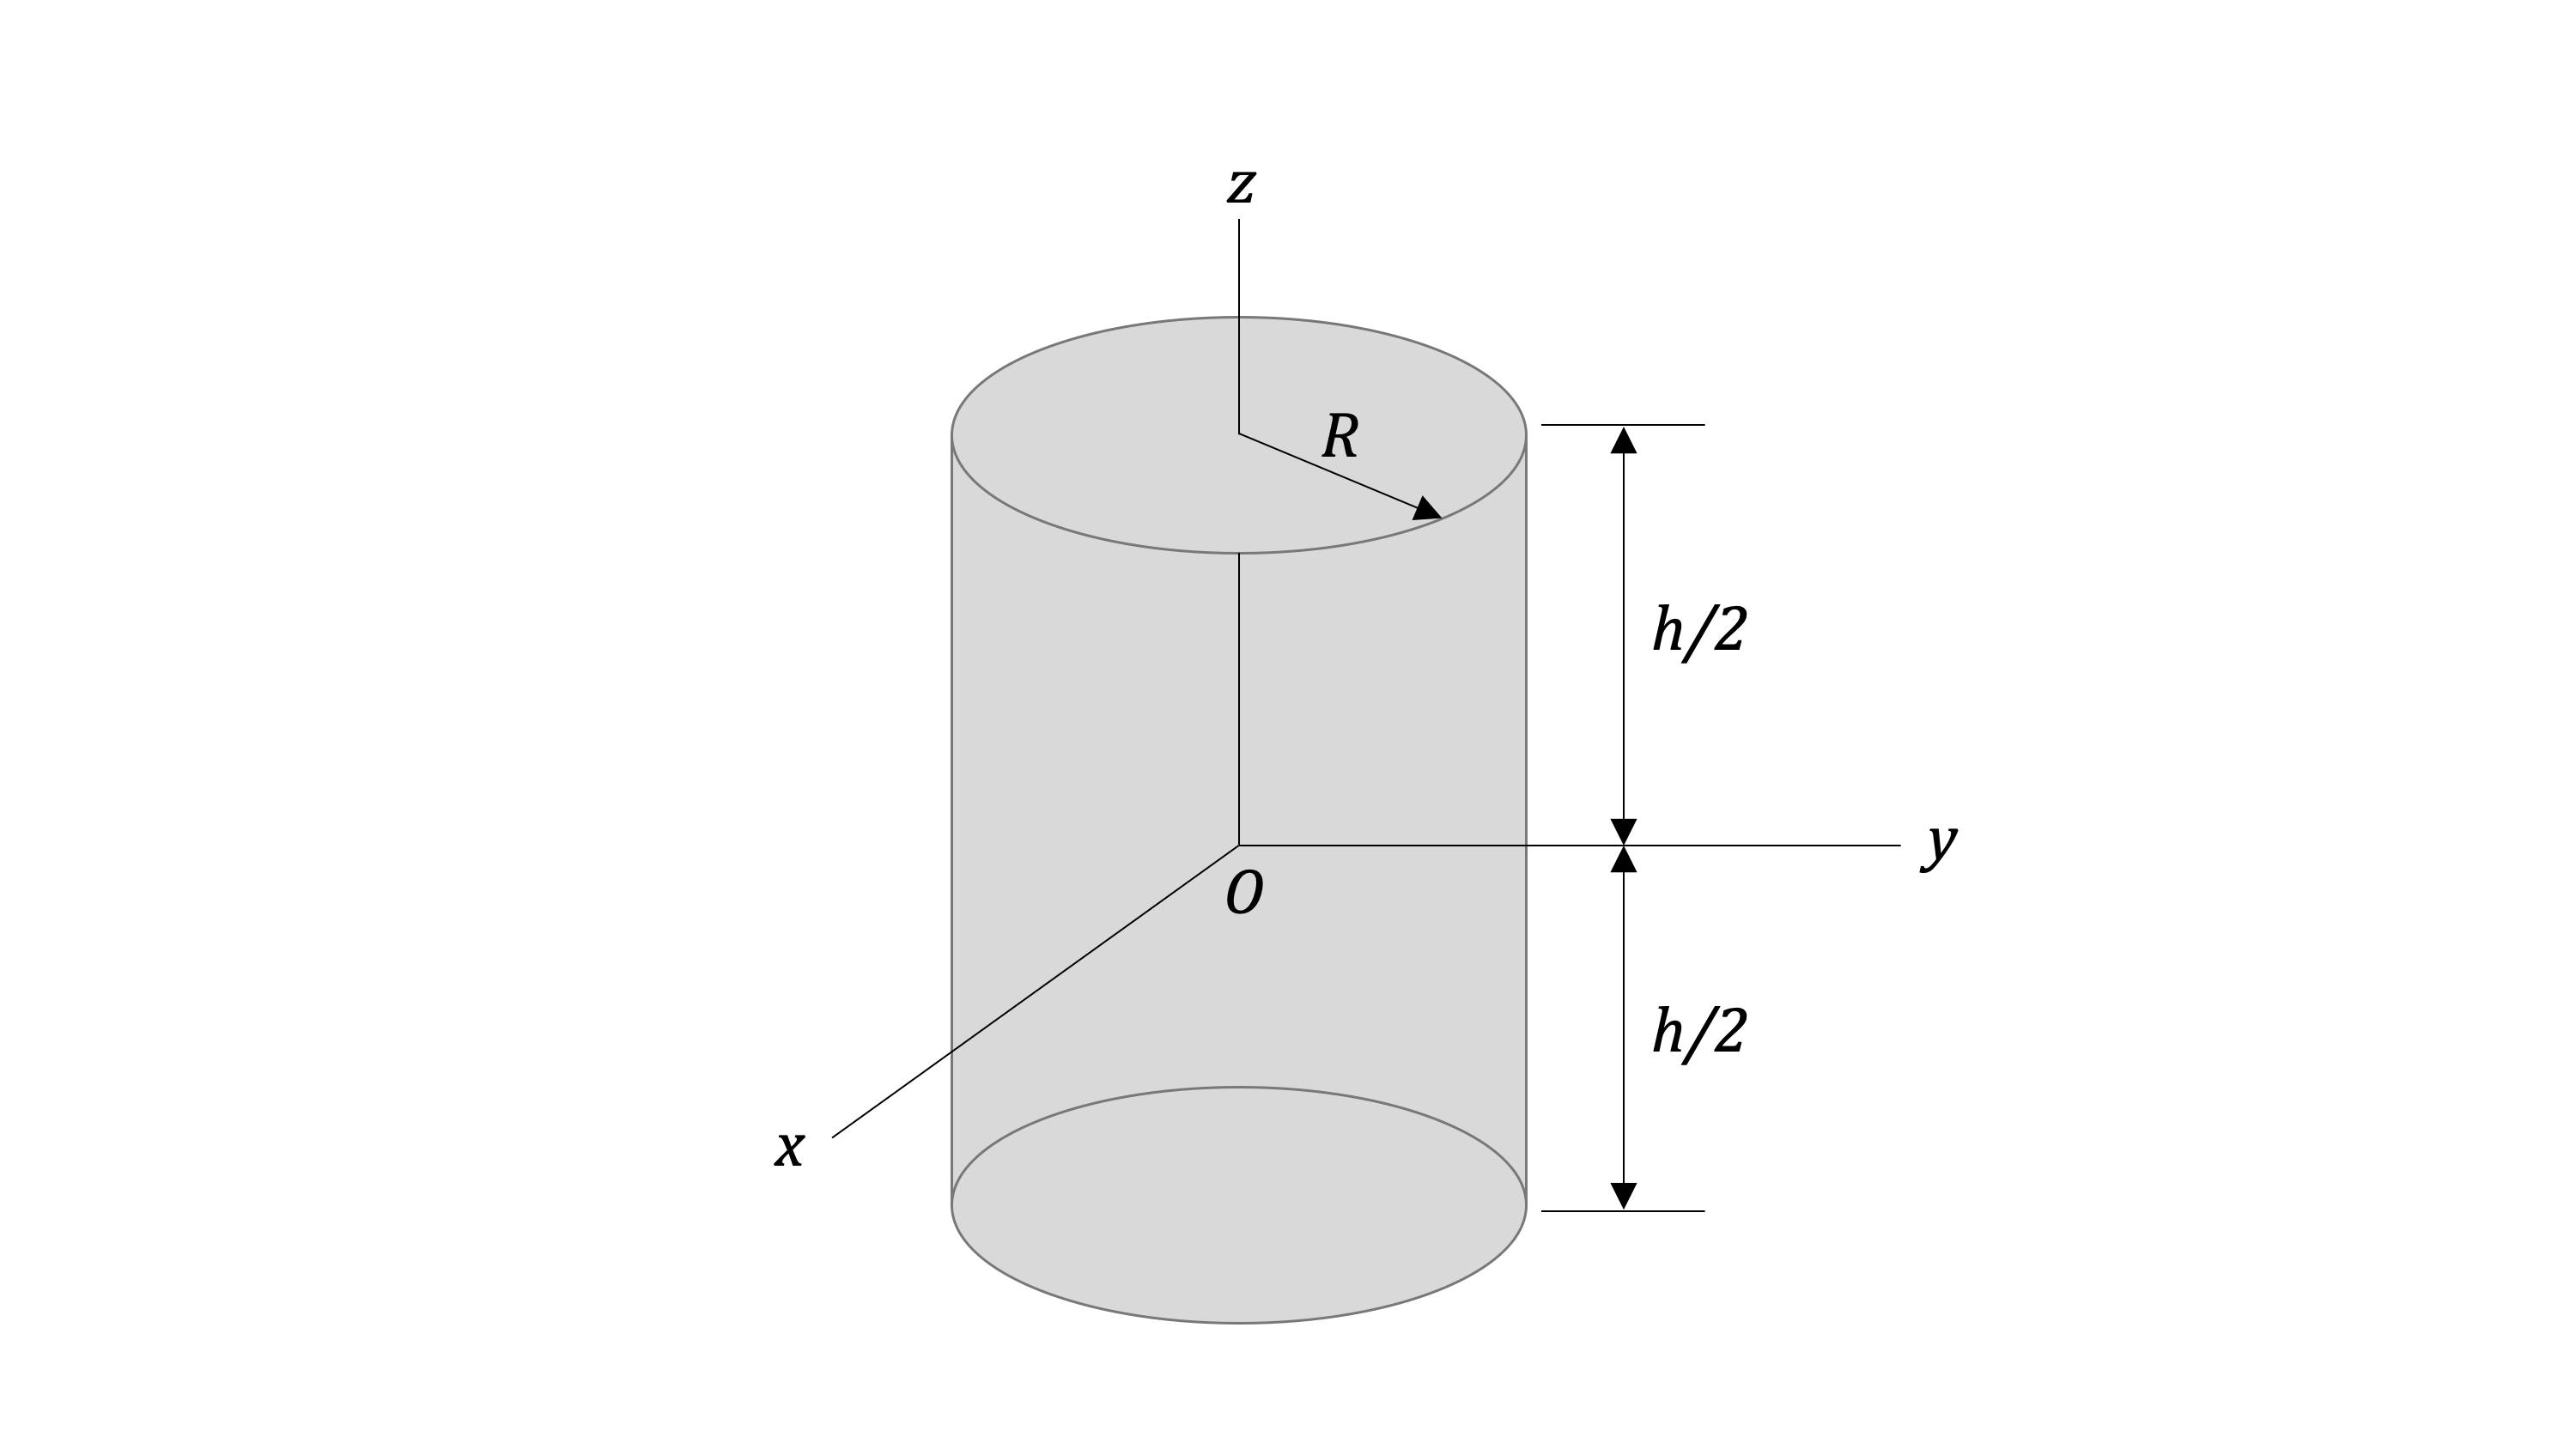
\includegraphics[trim={8cm 1cm 5cm 1.5cm},clip,width=0.4\textwidth, left]{Slide45} 

The mass moment of inertia has units of $mass \times distance^2$,  such as $kg{\text -}m^2$ or $slug{\text -}ft^2$.  It is always positive. 


\subsection{Example}

Find the mass moments of inertia about both the end and the center of mass of a uniform thin bar.

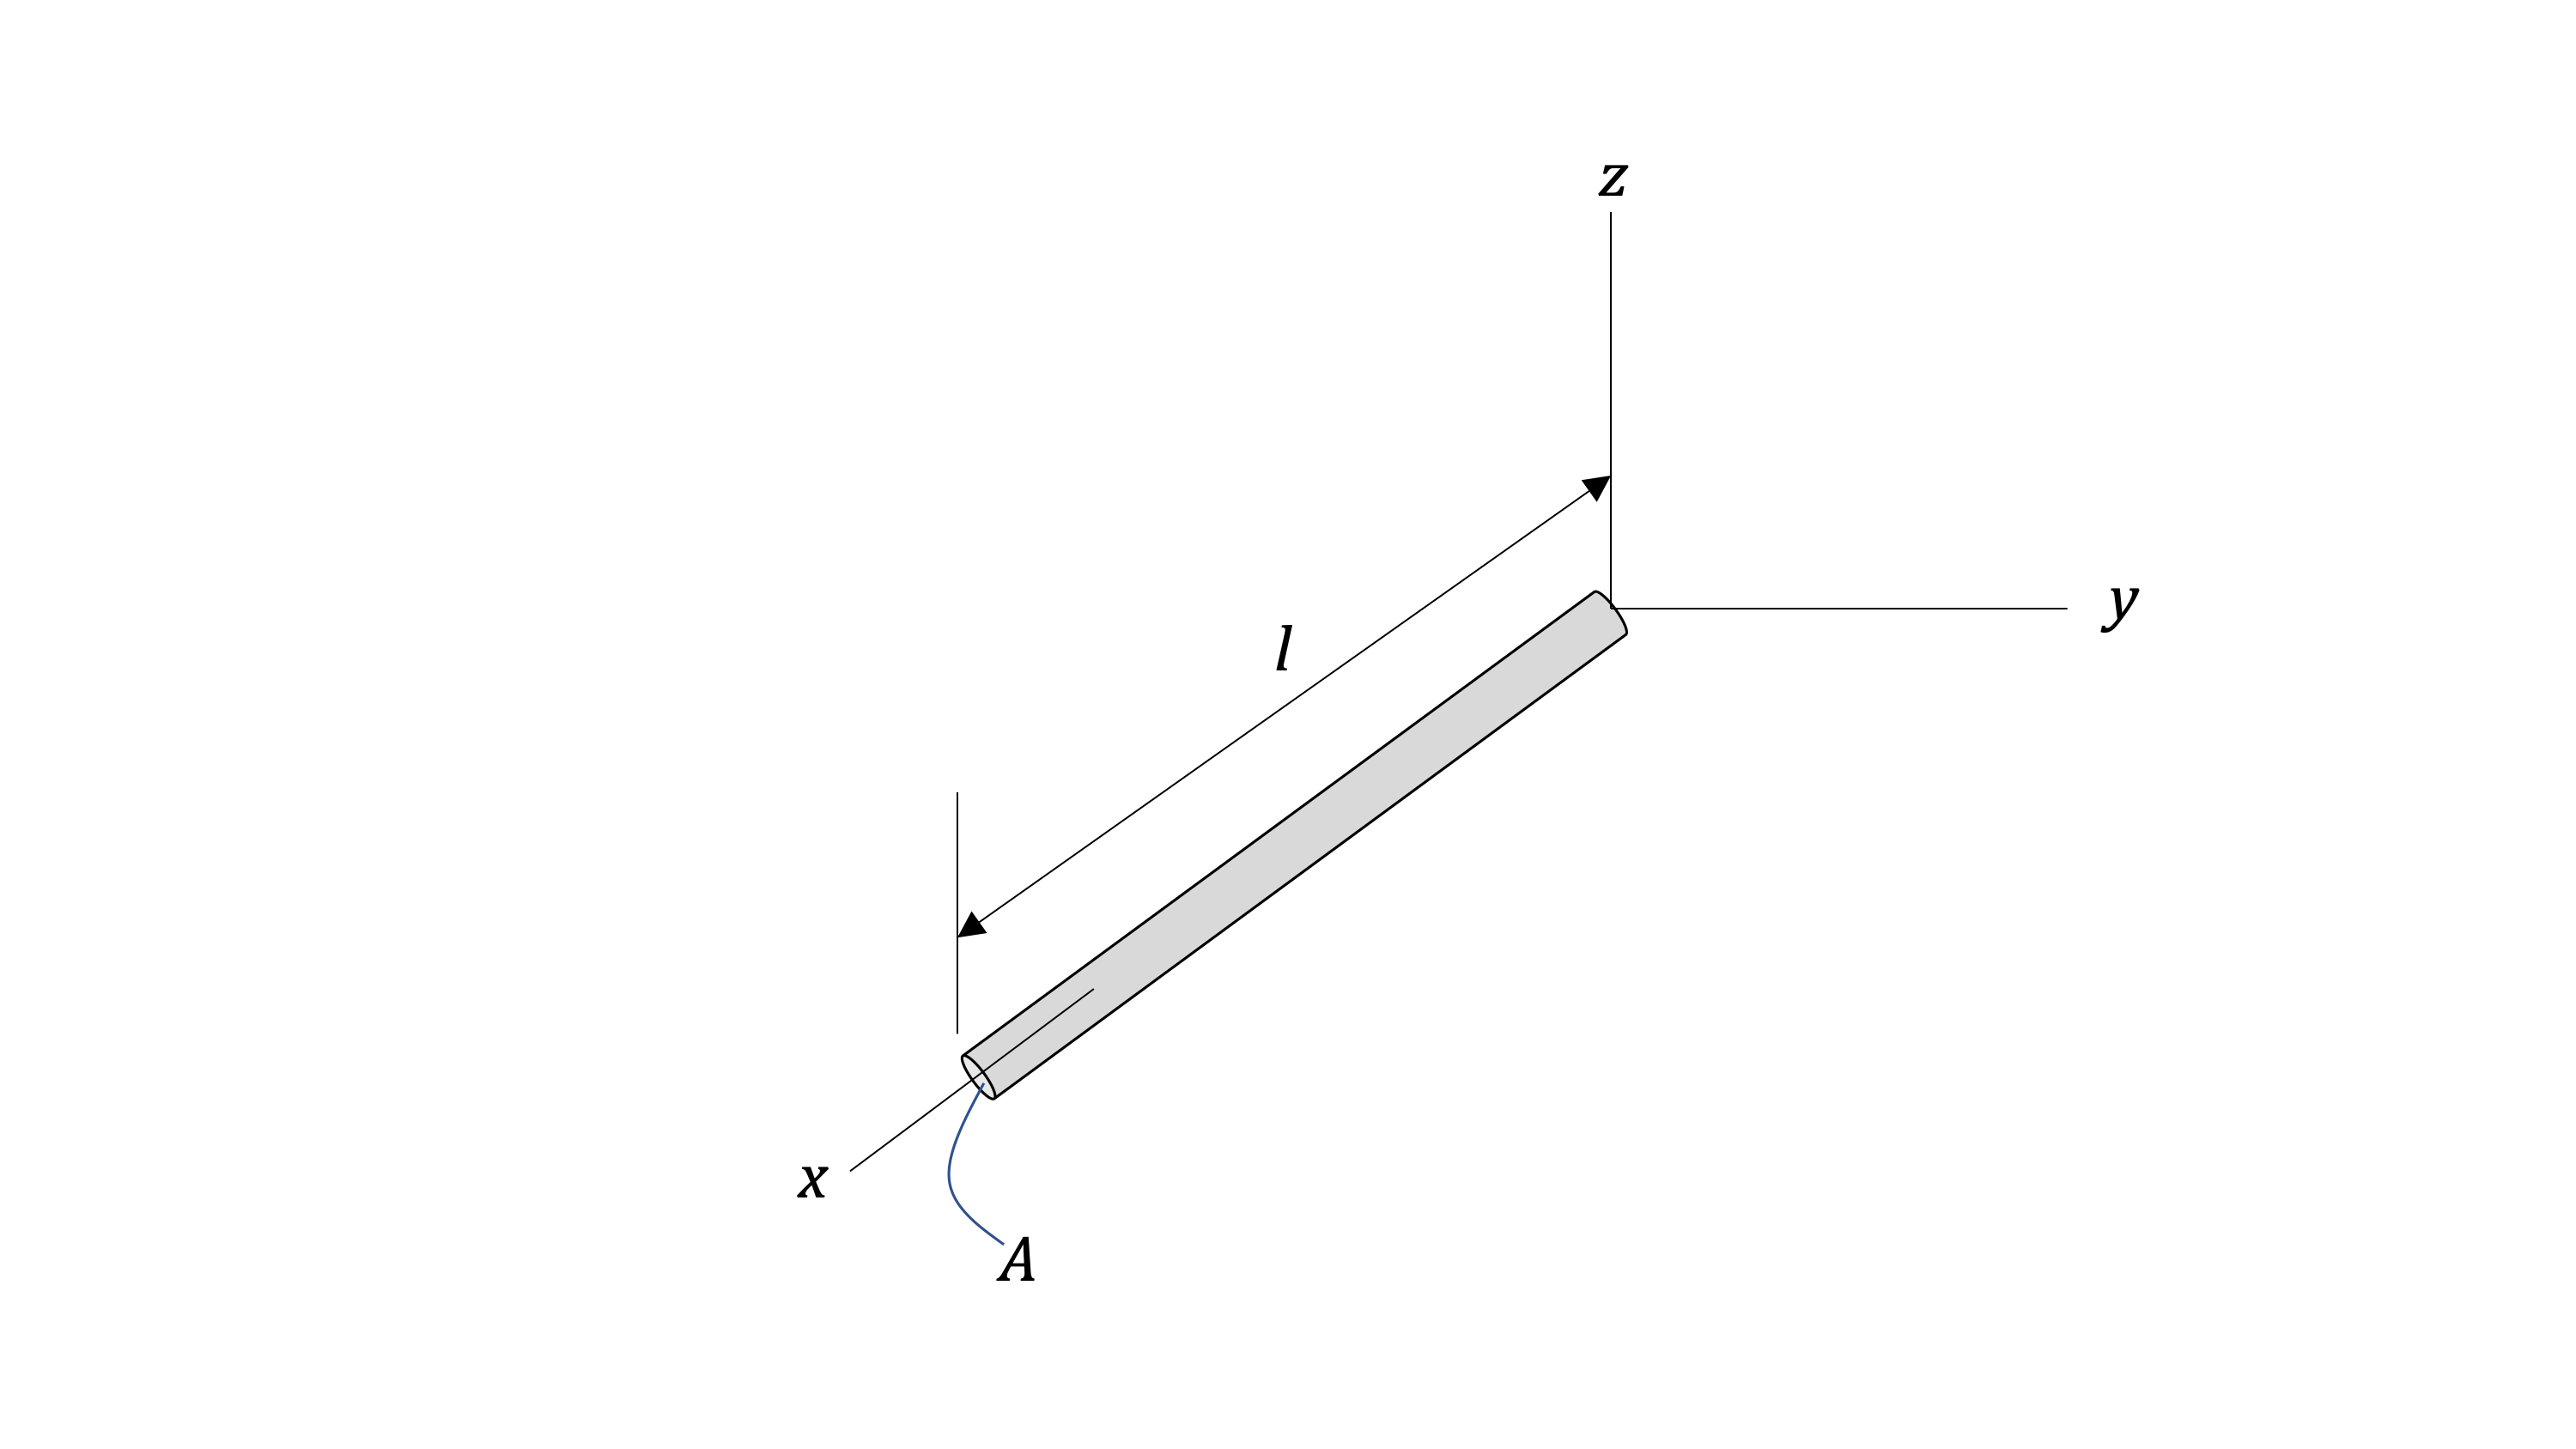
\includegraphics[trim={8cm 1cm 5cm 1.5cm},clip,width=0.4\textwidth, left]{Slide46} 

\vspace*{10\baselineskip}

\newpage

\section{Parallel Axis Theorem}
If the moment of inertia, $I_G$, of a body of mass, $m$, about an axis passing through the body’s centre of mass, $G$, is known, then the moment about any other parallel axis, distance, $d$, from $G$ can be found as:

\[I_{parallel axis} = I_G + m d^2\]

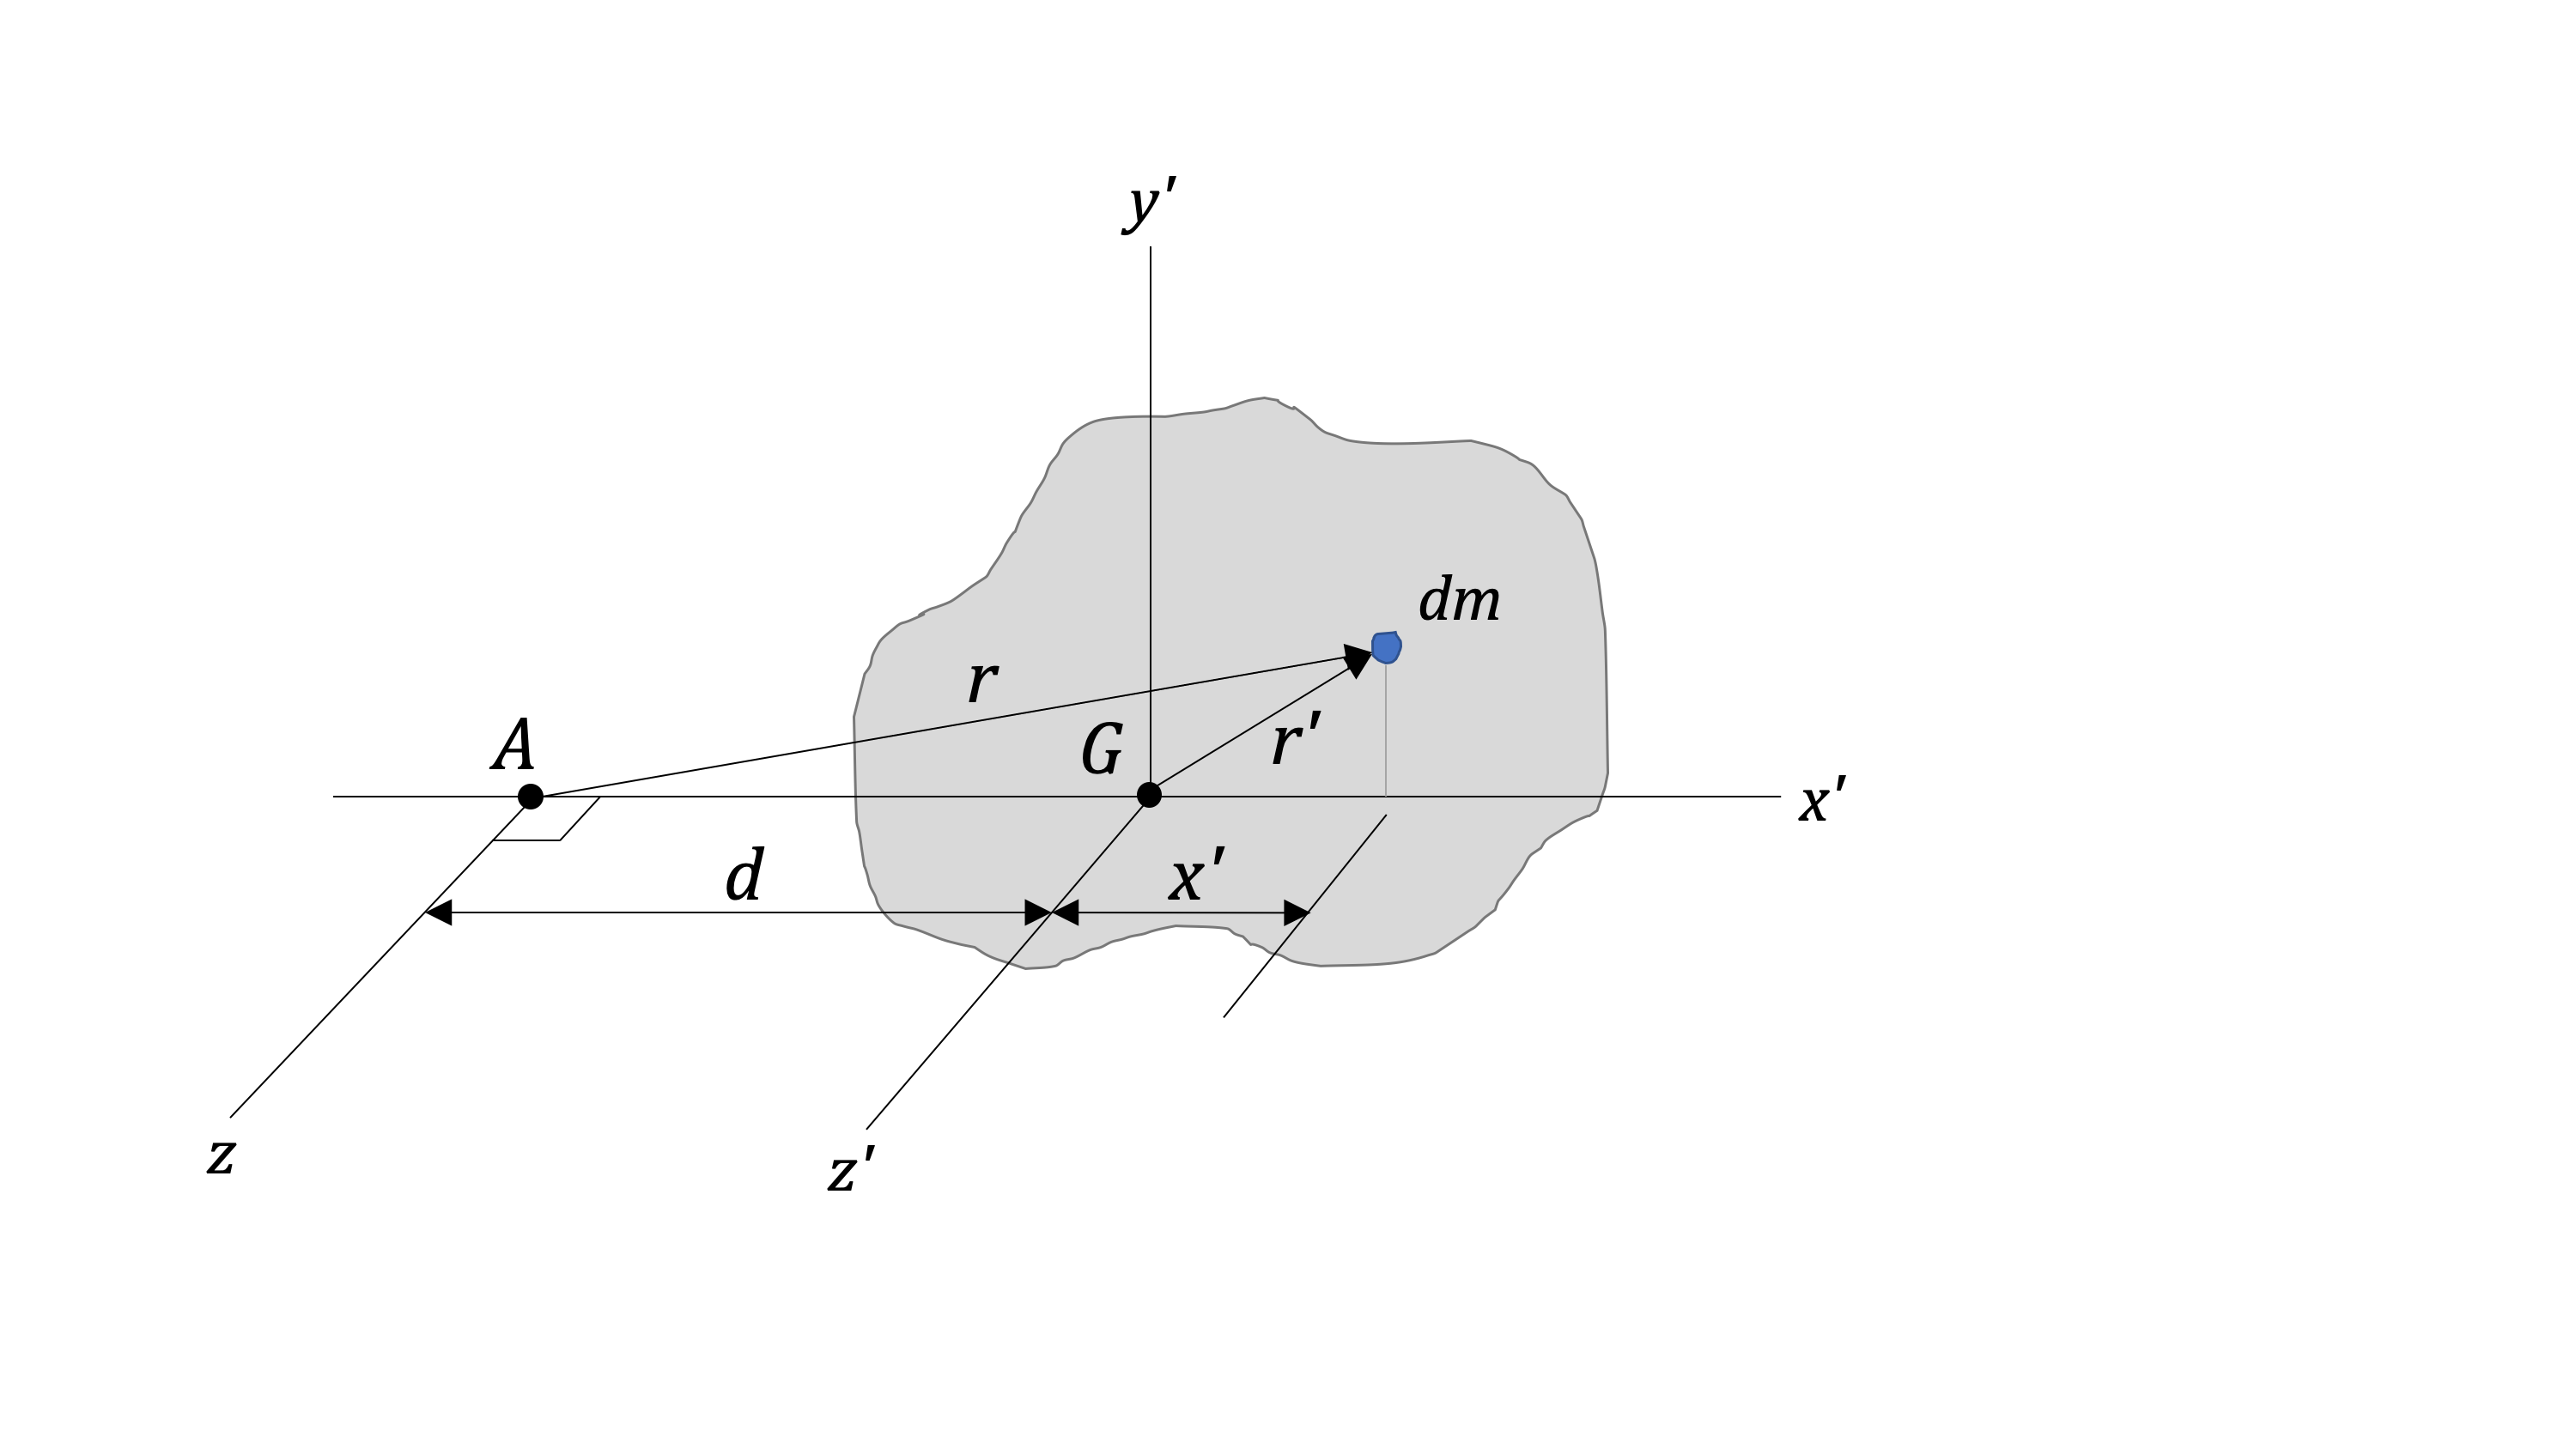
\includegraphics[trim={1cm 2cm 7cm 1.5cm},clip,width=0.7\textwidth, left]{Slide47} 

This theorem can also be applied to second moments of area, i.e.:

\[
I_x= I_{Cx'} + A d_y^2
\]
\[
I_y= I_{Cy'} + A d_x^2
\]
\[
J_O= J_{C} + A d^2
\]

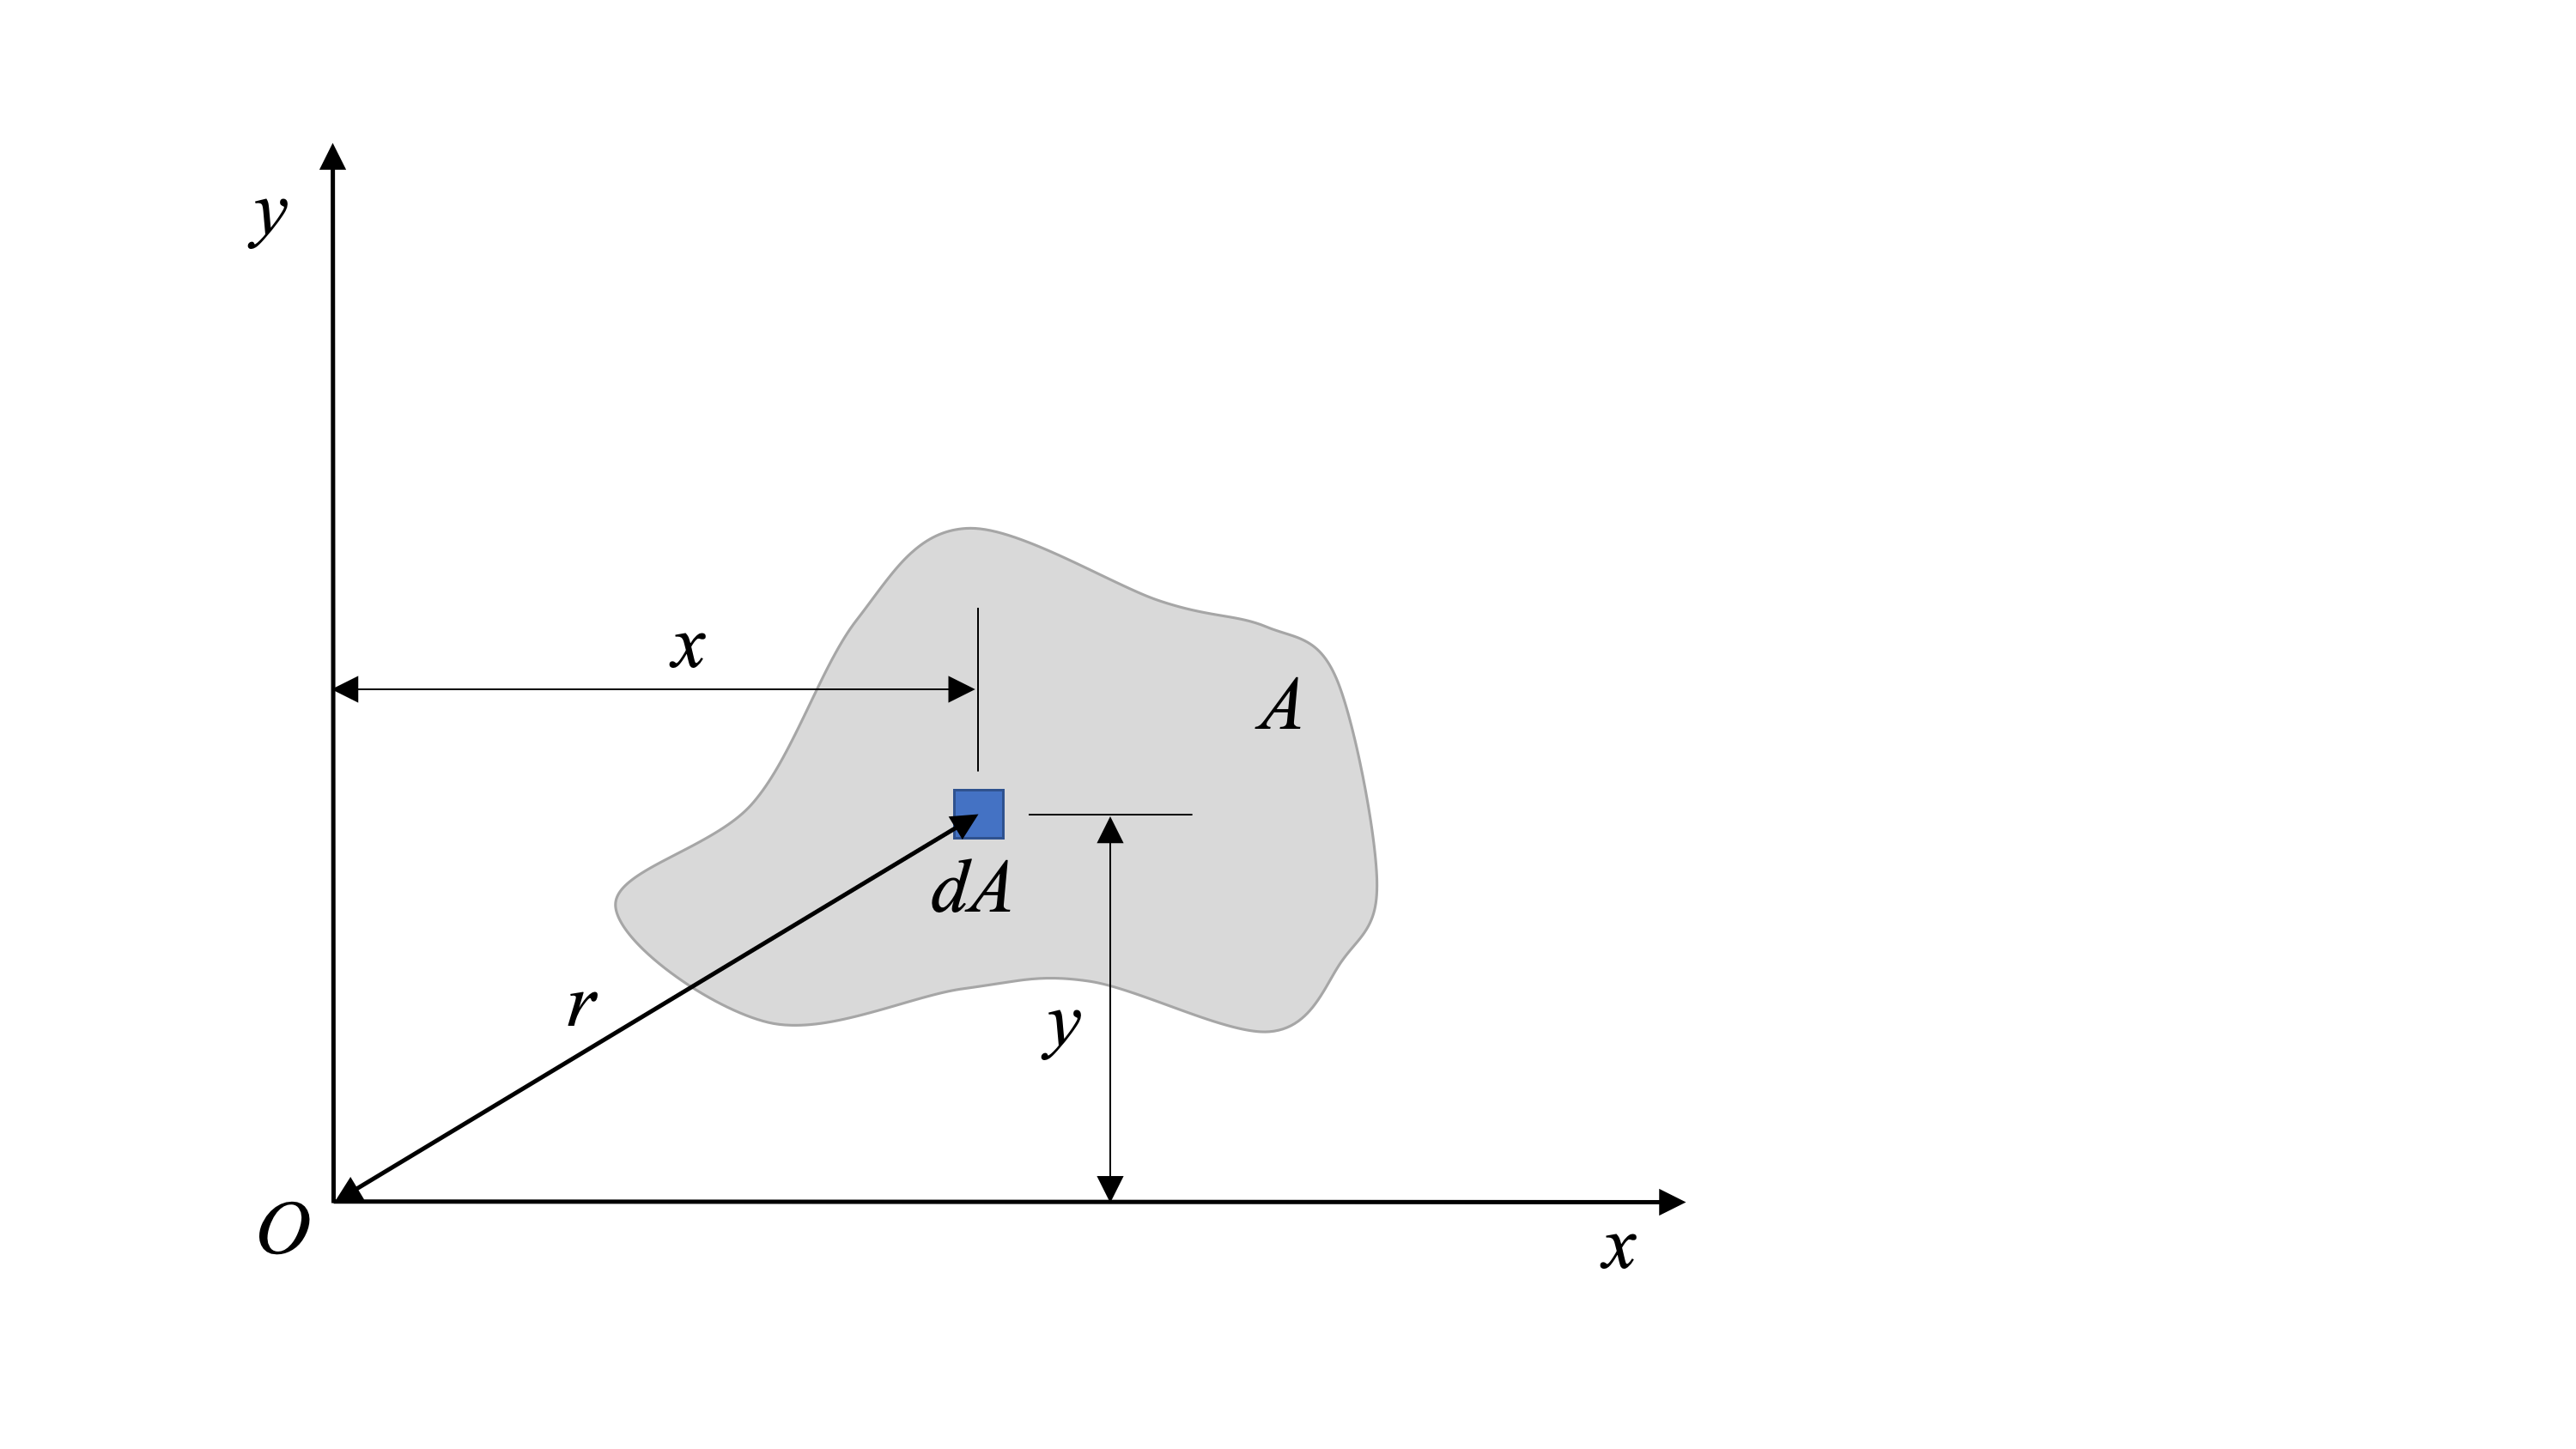
\includegraphics[trim={1cm 1cm 4cm 1cm},clip,width=0.6\textwidth, center]{Slide42} 

\newpage

\subsection{Example}
Find the mass moment of inertia of the plate about point $O$.  The plate has thickness $50 \, mm$ and density $50 \, kg/m^3$.

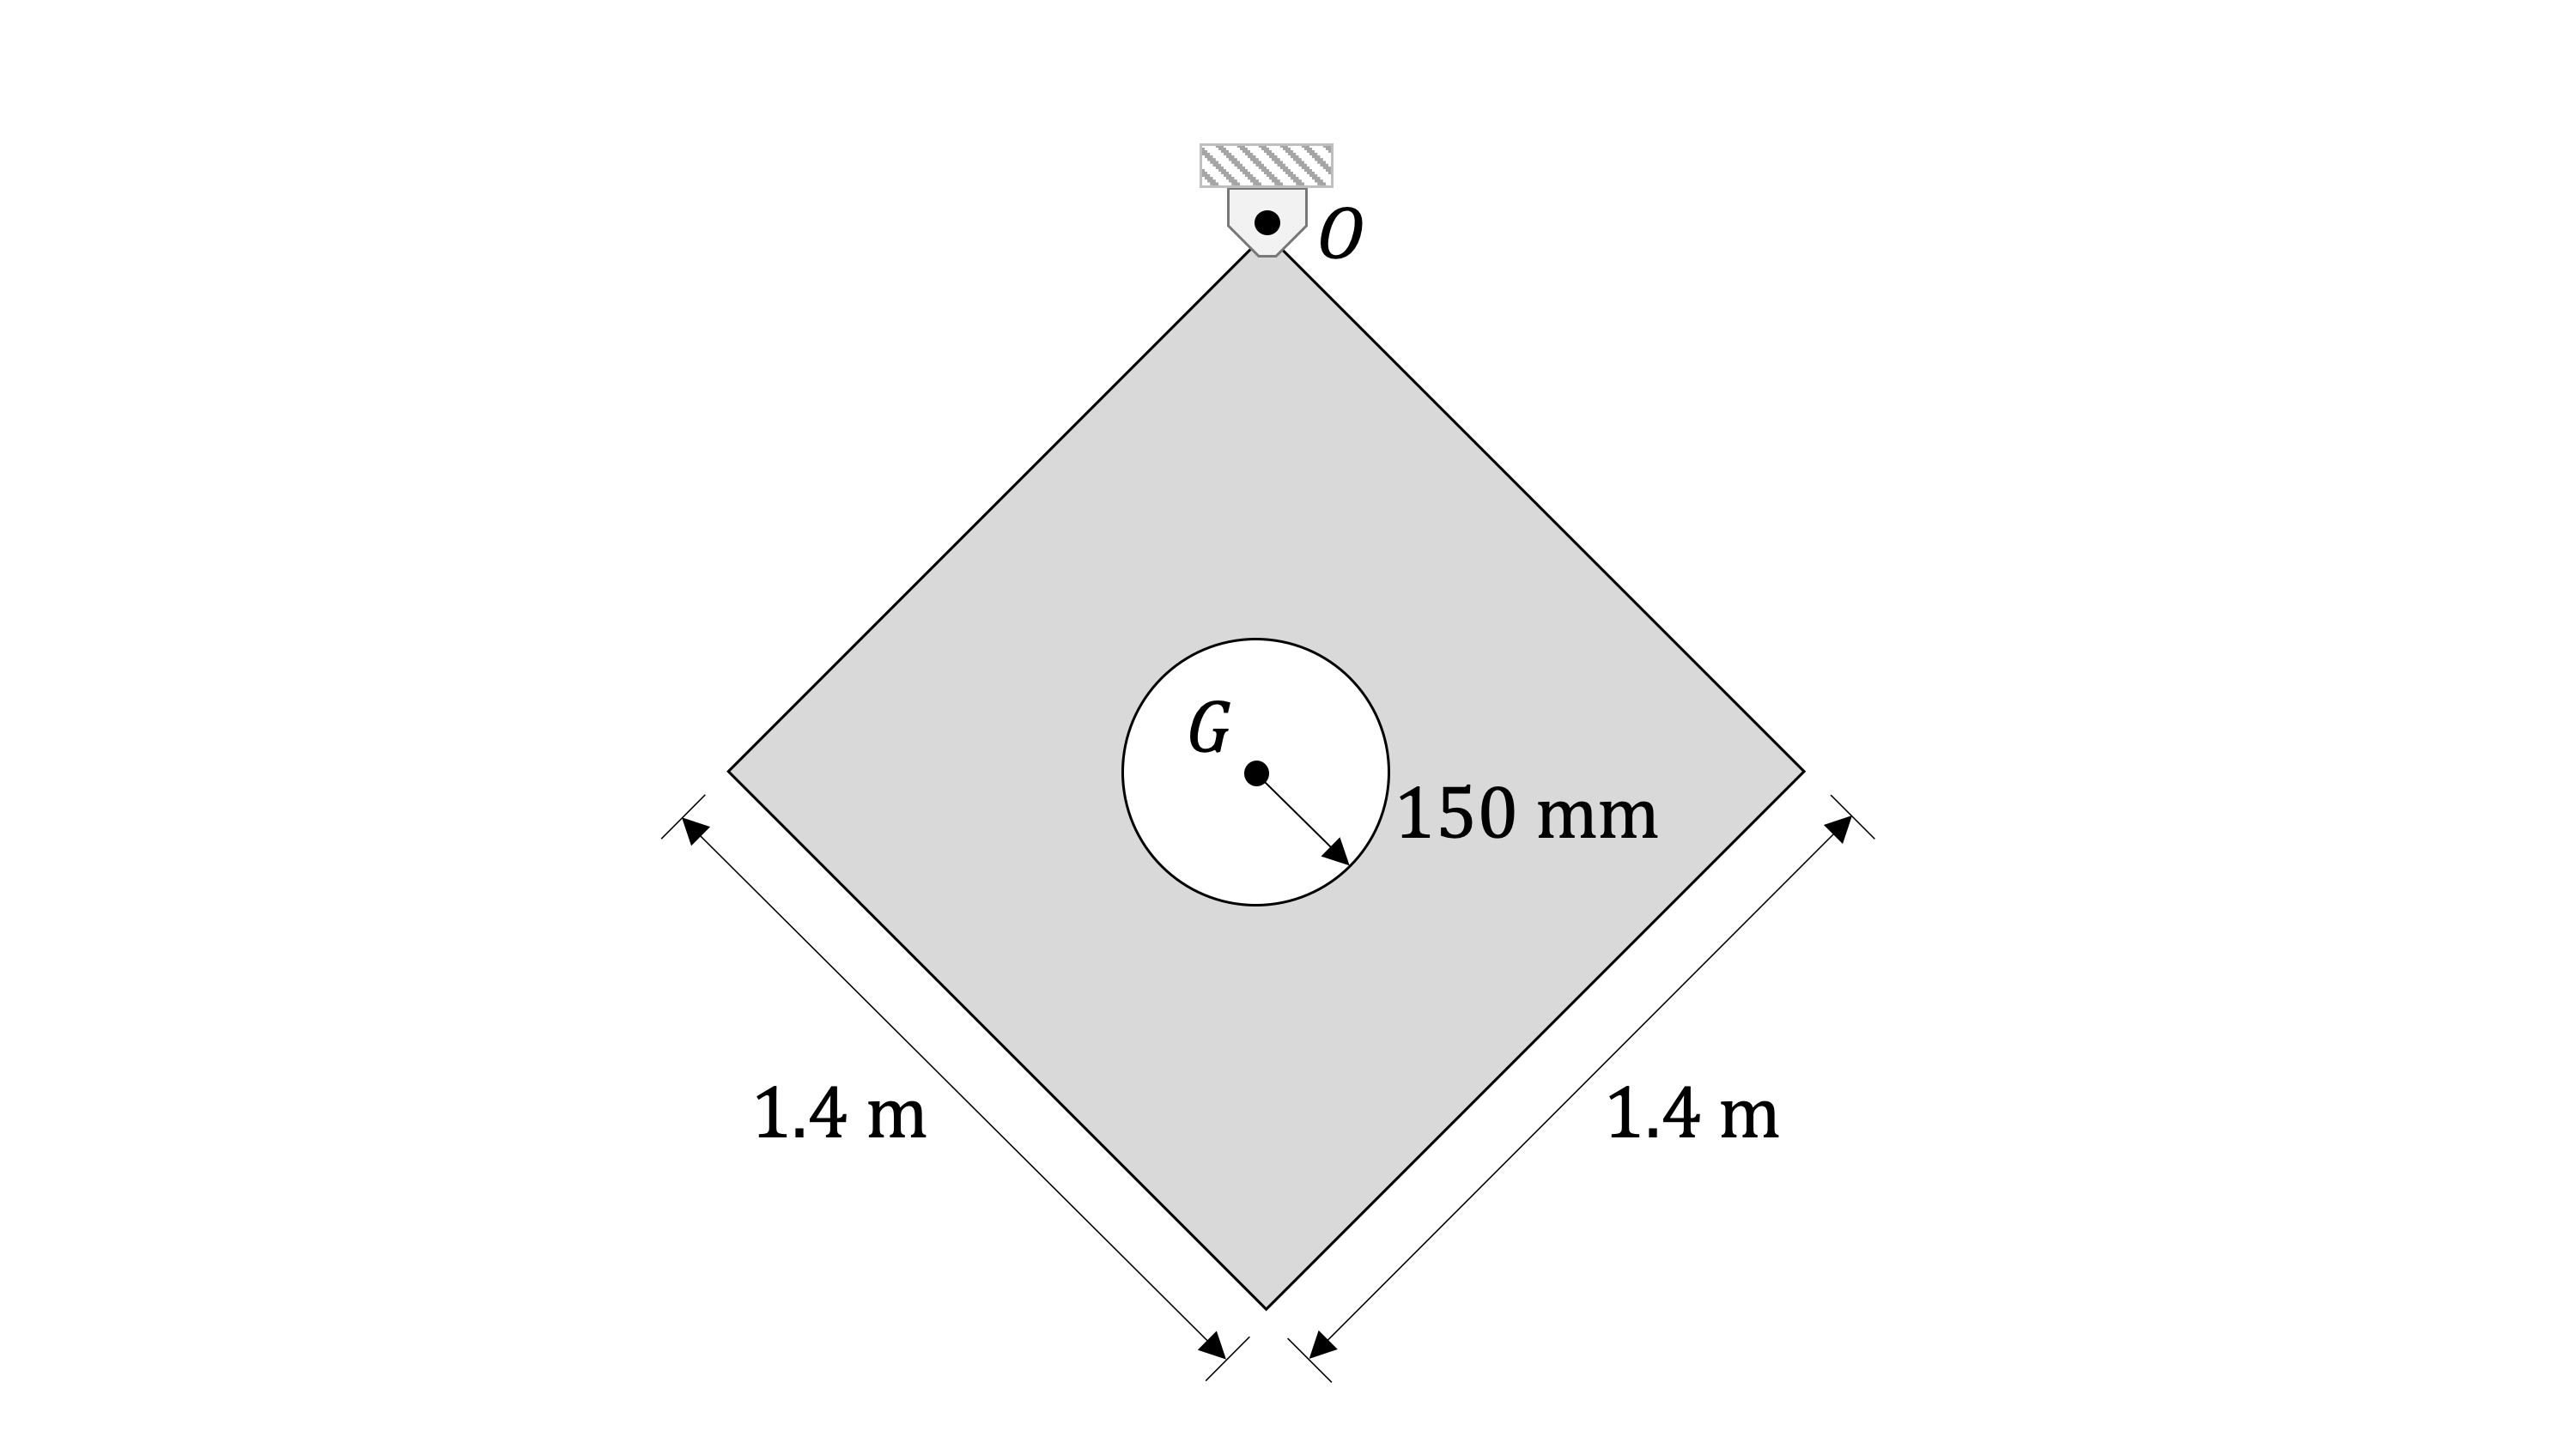
\includegraphics[trim={6cm 1cm 5cm 1cm},clip,width=0.5\textwidth, left]{Slide48} 

\vspace*{10\baselineskip}

\newpage

\section{Radius of Gyration}
The radius of gyration, $k_G$, is a method of specifying the inertia of a body without including the mass.  It is specified in units of length.  Using this measure, the mass moment of inertia of a body is:

\[
I = mk_G^2 \hspace{1 cm} or \hspace{1 cm} \displaystyle k_G = \sqrt{\frac{I}{m}}
\]

One can specify the radius of gyration for the second moment of area by substituting area, $A$, for mass $m$.

For a circular ring the radius of gyration about the centroidal axis normal to the ring is the same as the radius of the ring.

\newpage

\section{Summary}
\begin{center}
\begin{tabu} to 1\textwidth {  | X[1, l]  | X[1, c] | X[1, l] | }
\hline
 & & \\
Centroid & $\displaystyle \bm{r_C} =\frac{\displaystyle  \iint_A \bm{r} dA}{A} $ & Same for uniform density material\\

Centre of Mass & $\displaystyle \bm{r_G} =\frac{\displaystyle  \iint_m \bm{r} dm}{m} $ &  \\
& & \\
\hline
& & \\
Second Moment of Area (moment of inertia) about an axis (area in the x,y plane) & $I_x= I_{Cx'} + A d_y^2$ $I_y= I_{Cy'} + A d_x^2$ $J_O= J_{C} + A d^2$ & 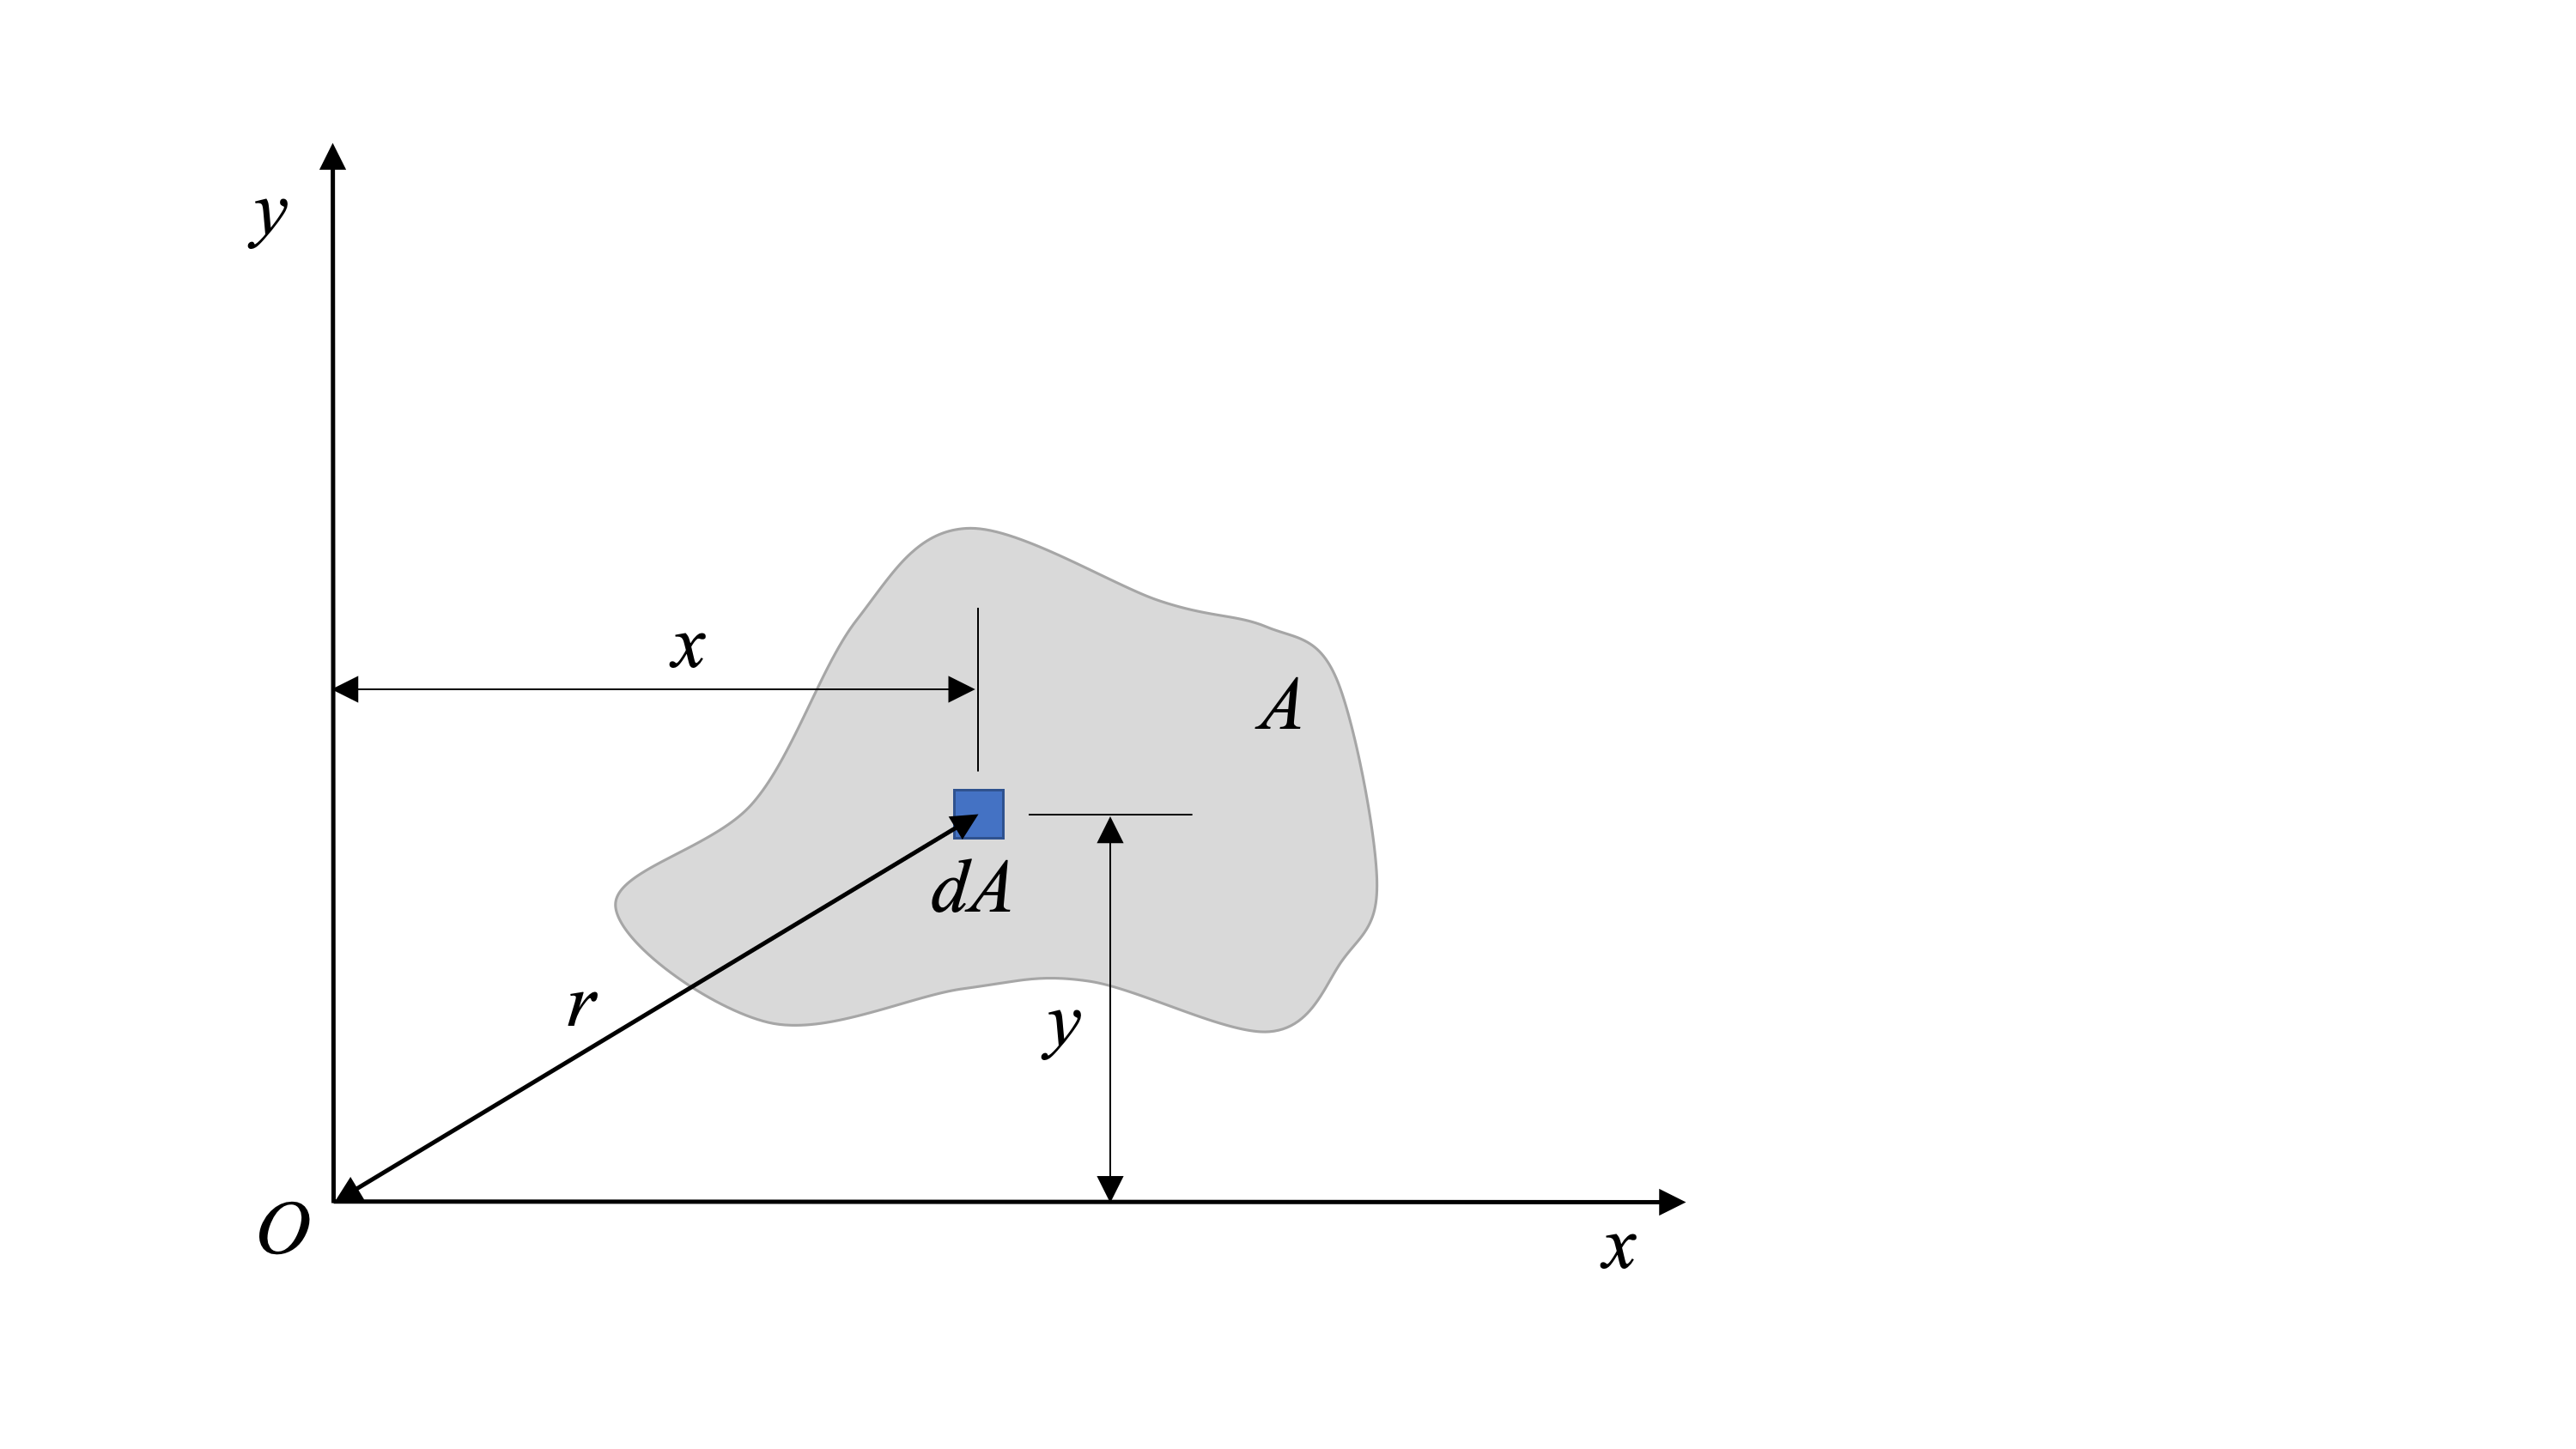
\includegraphics[trim={1cm 2cm 8cm 1cm},clip,width=2.3in]{Slide42}\\
& & \\
\hline
& & \\
Mass Moment of Inertia about an axis & $\displaystyle I =  \iint_m \bm{r}^2 dm$ & 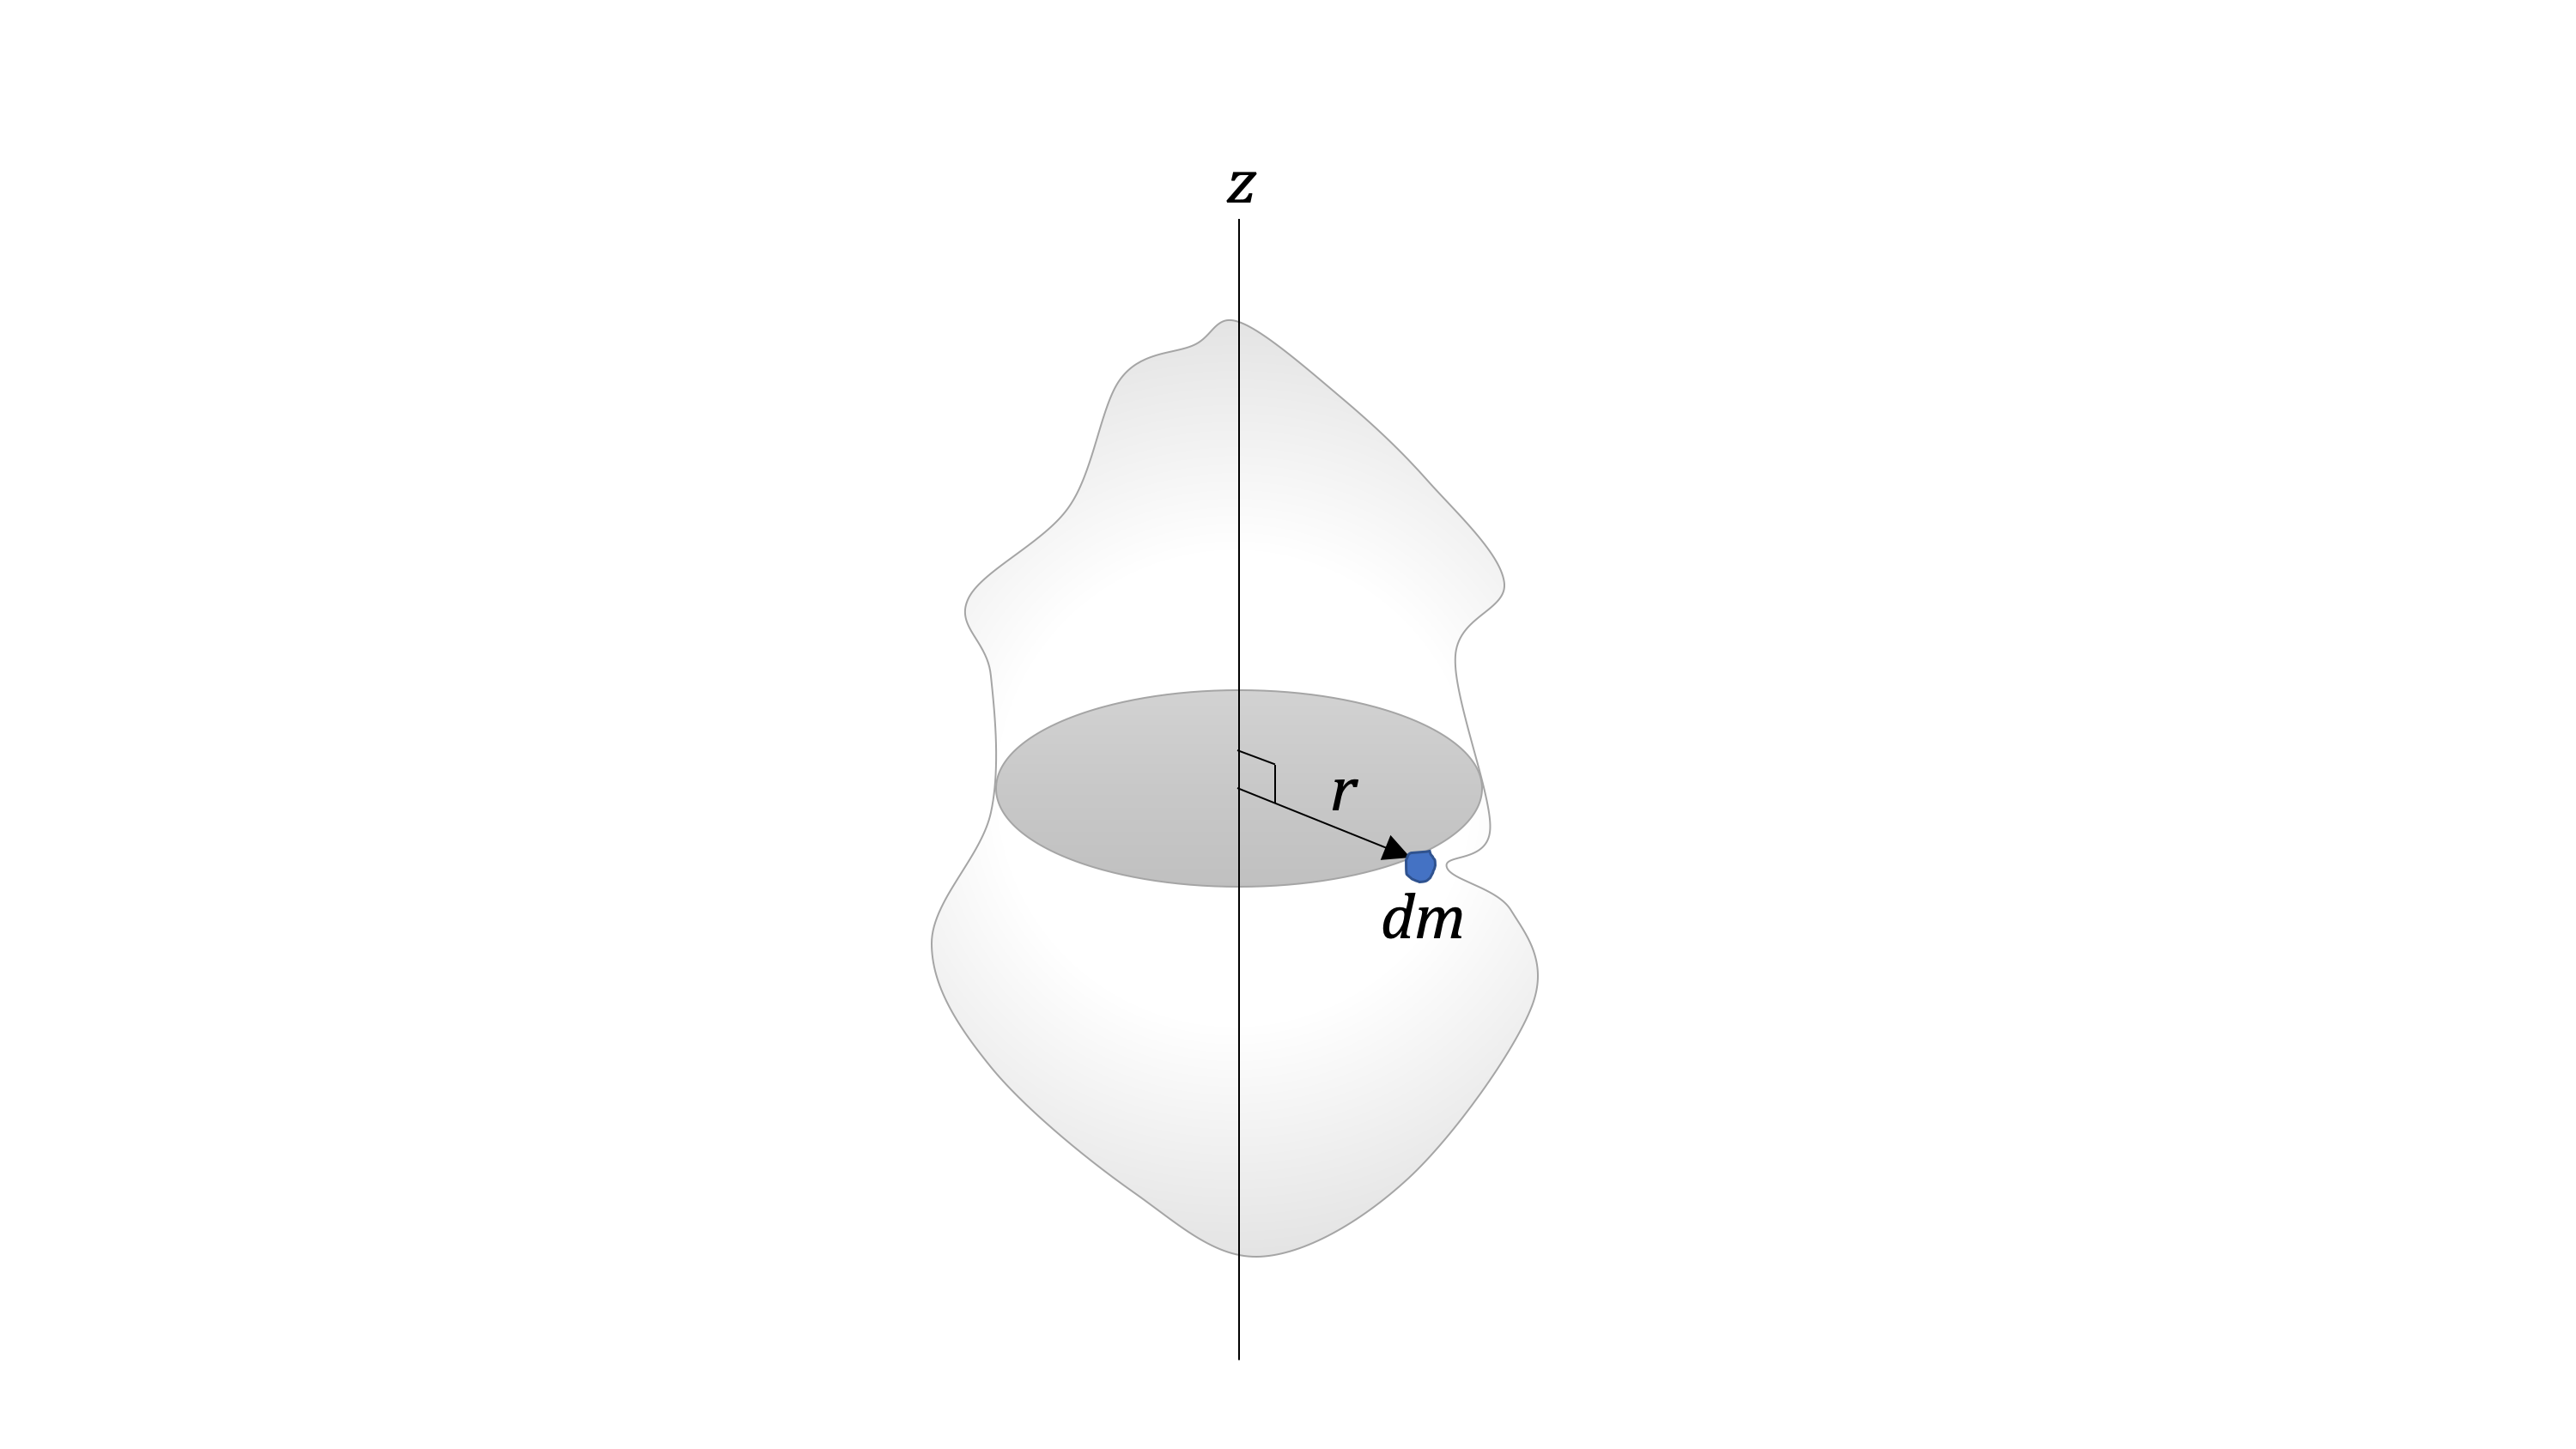
\includegraphics[trim={8cm 1cm 5cm 1.5cm},clip,width=2.3in]{Slide44}\\
& &\\
\hline
& &\\
For a planar body of uniform thickness and density & $\displaystyle I_{zz} = \rho h (I_x + I_y) = \rho h J_O$ & \\
& &\\
\hline
\end{tabu}
\begin{tabu} to 1\textwidth {  | X[1, l]  | X[1, c] | X[1, l] | }
\hline
& & \\
Parallel Axis Theorem & $I_x= I_{Cx'} + A d_y^2$ $I_y= I_{Cy'} + A d_x^2$ $J_O= J_{C} + A d^2$ $I_{parallel\,axis} = I_G + m d^2$ & 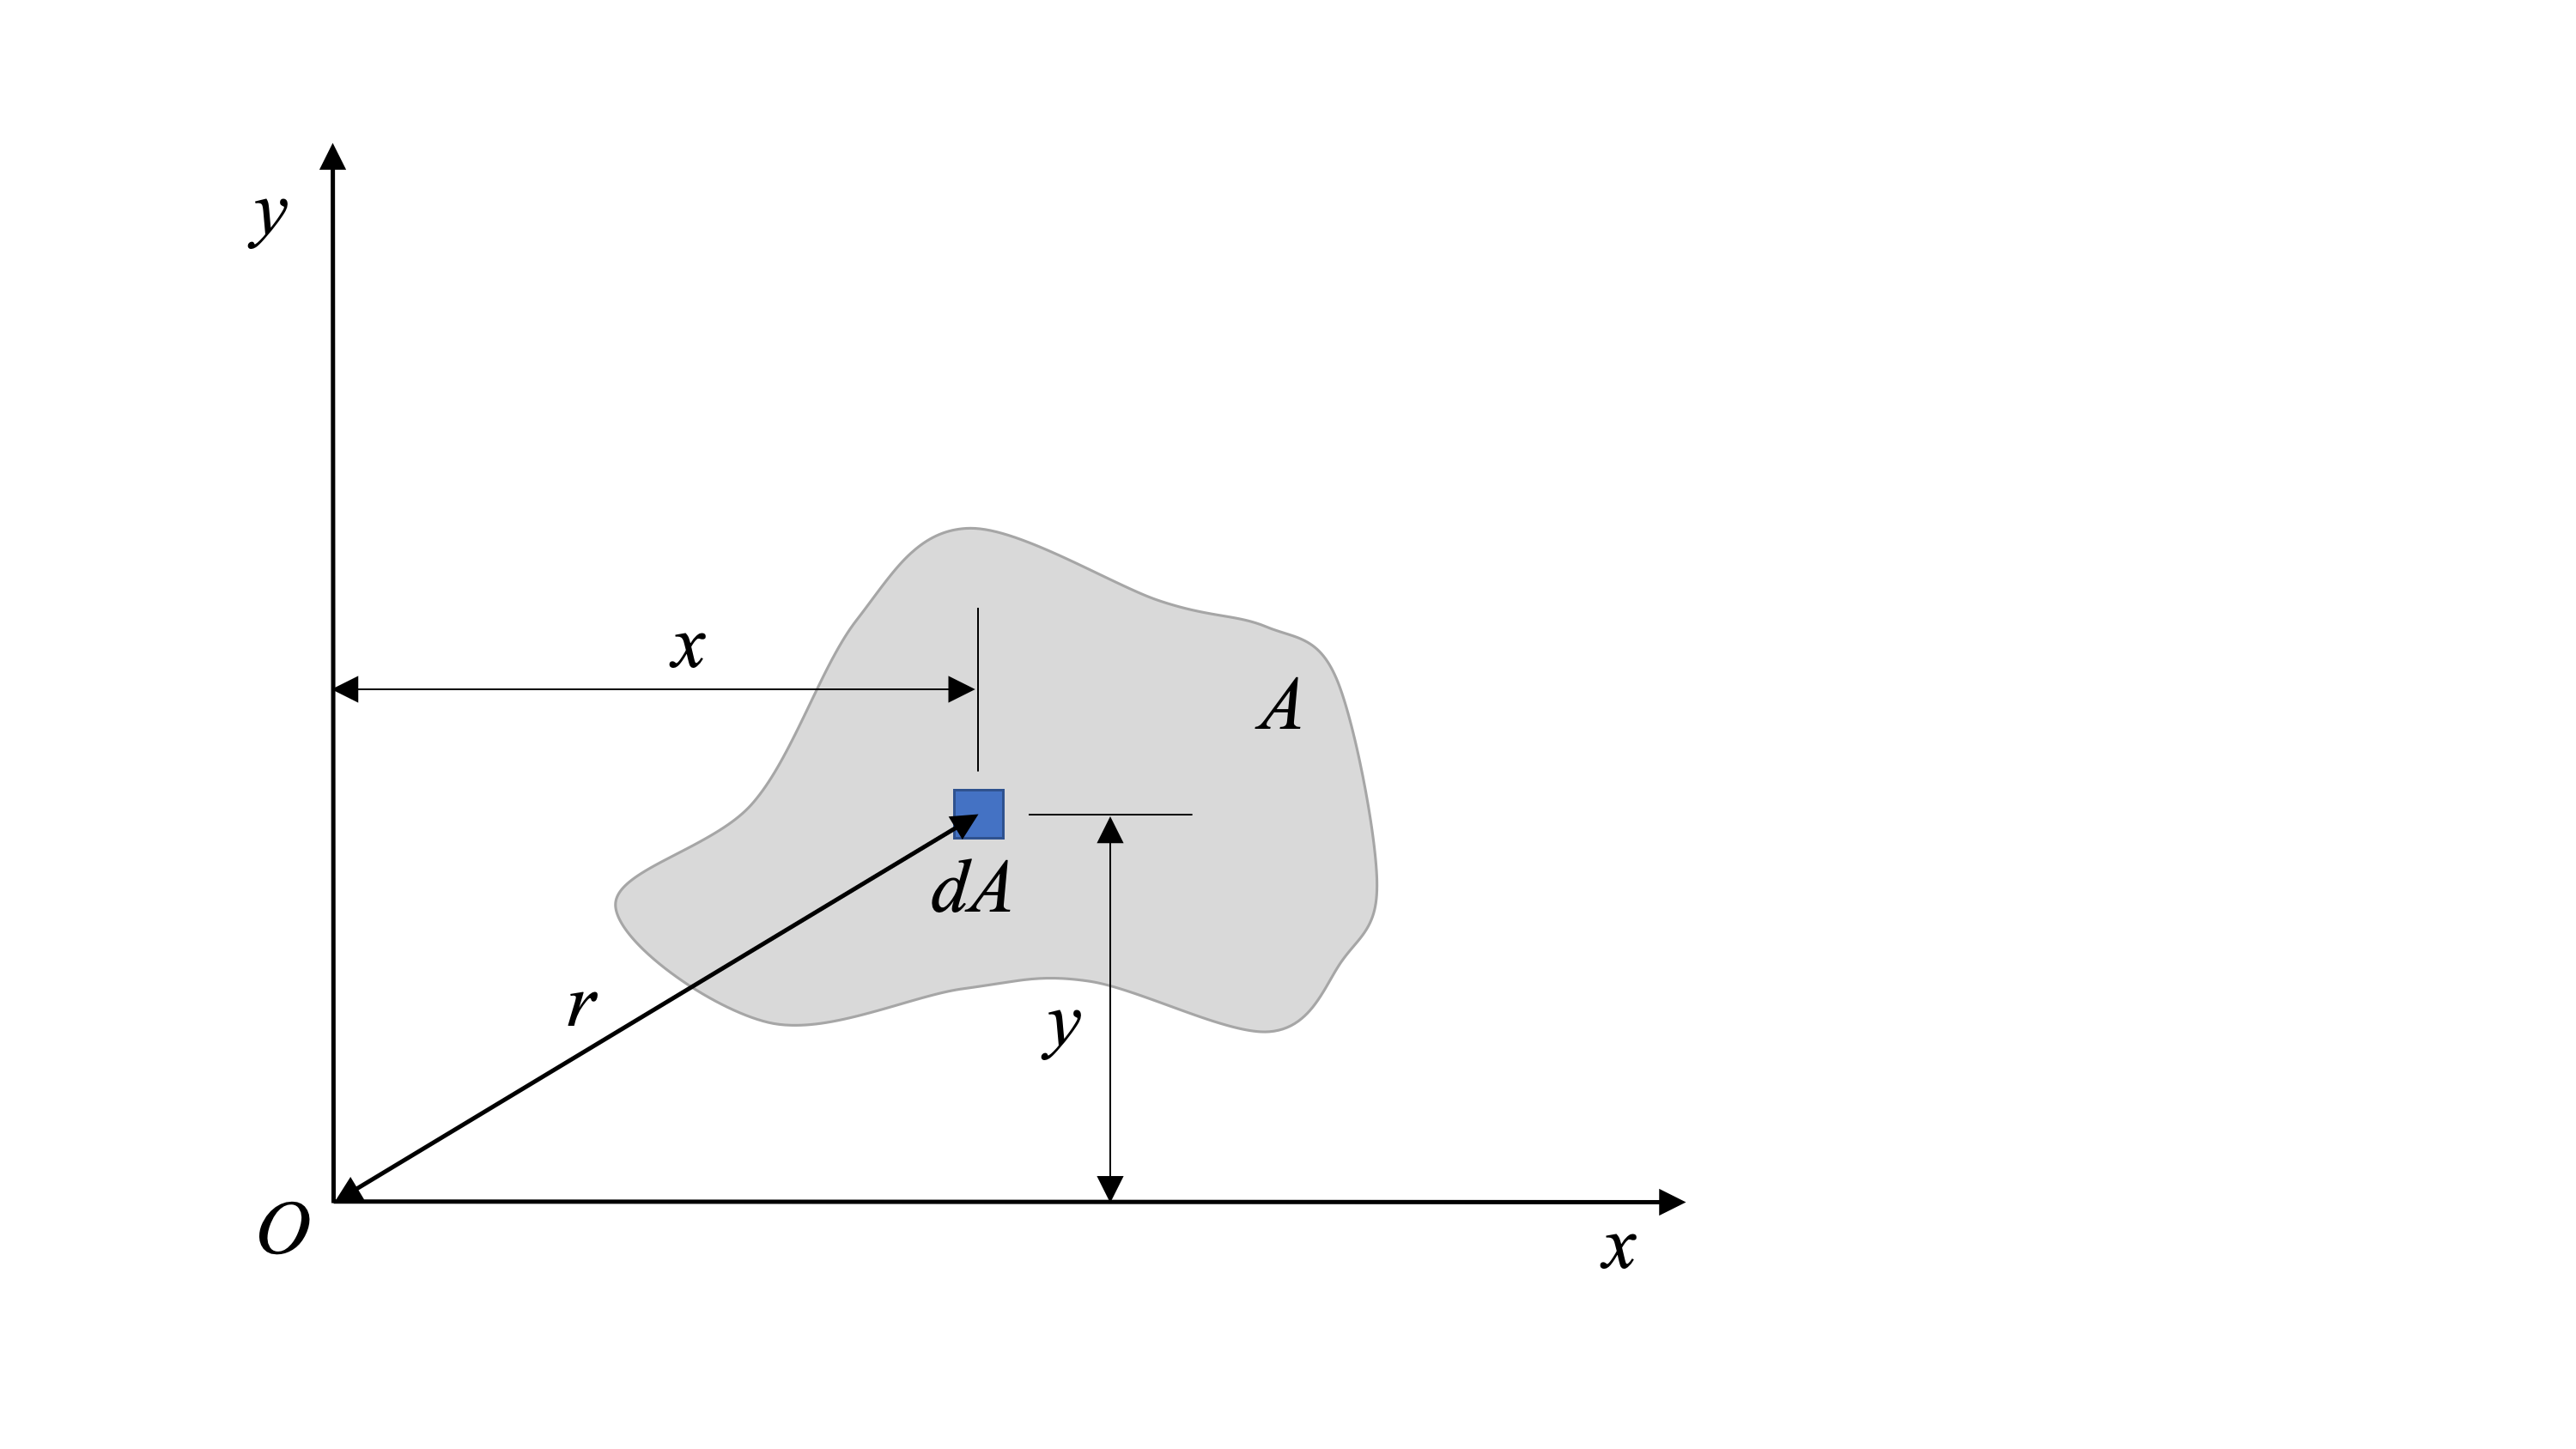
\includegraphics[trim={1cm 2cm 8cm 1cm},clip,width=2.3in]{Slide42}\\
& &\\
\hline
& &\\
Radius of Gyration & $I = mk_G^2 \hspace{1 cm}$ or $\hspace{1 cm}\displaystyle k_G = \sqrt{\frac{I}{m}}$ & For second moment of area, replace m with A\\
& &\\
\hline
\end{tabu}
\end{center}

\newpage

\chapter{L10/L11: Introduction to Rigid Body Kinetics}
Readings

\section{Objective}
To apply Newton’s Second Law to \textbf{planar} rigid bodies.  This mean’s that we need to account for the fact that the body be considered is NOT a point mass.  We will use the concepts of Centre of Mass and Inertia, established in the previous lecture.

\section{Review – Newton’s Second Law}
A particle acted on by an unbalanced force, $\bm{F}$, experiences an acceleration, $\bm{a}$, in the same direction as the force, and a magnitude that is directly proportional to the force.

\vspace*{7\baselineskip}

\[ 
\bm{F} = m\bm{a} \hspace{1 cm} \text{or} \hspace{1 cm} \bm{F} - m\bm{a} = 0
\]

$\bm{F}$ is a vector that represents the resultant of all forces acting on the body.  

Thus, depending on the coordinate system selected, for a particle we would have the following set of equations:

\begin{center}
\begin{tabu} to 1\textwidth {  | X[1, c]  | X[1, c] | X[1, c] | }
\hline
Cartesian & Normal/Tangential & Polar/Cylindrical\\
\hline
$\sum F_x = m a_x $ & $\sum F_n = m a_n $ & $\sum F_r = m a_r $\\
$\sum F_y = m a_y$ & $\sum F_t = m a_t$ & $\sum F_{\theta} = m a_{\theta}$\\
$\sum F_z = m a_z$ & $\sum F_b = 0$ &$\sum F_z = m a_z$ \\
\hline
\end{tabu}
\end{center}

\newpage

\section{Equations of Motion for a Planar Rigid Body}
Consider what this means for a planar body – which is a collection of particles. 

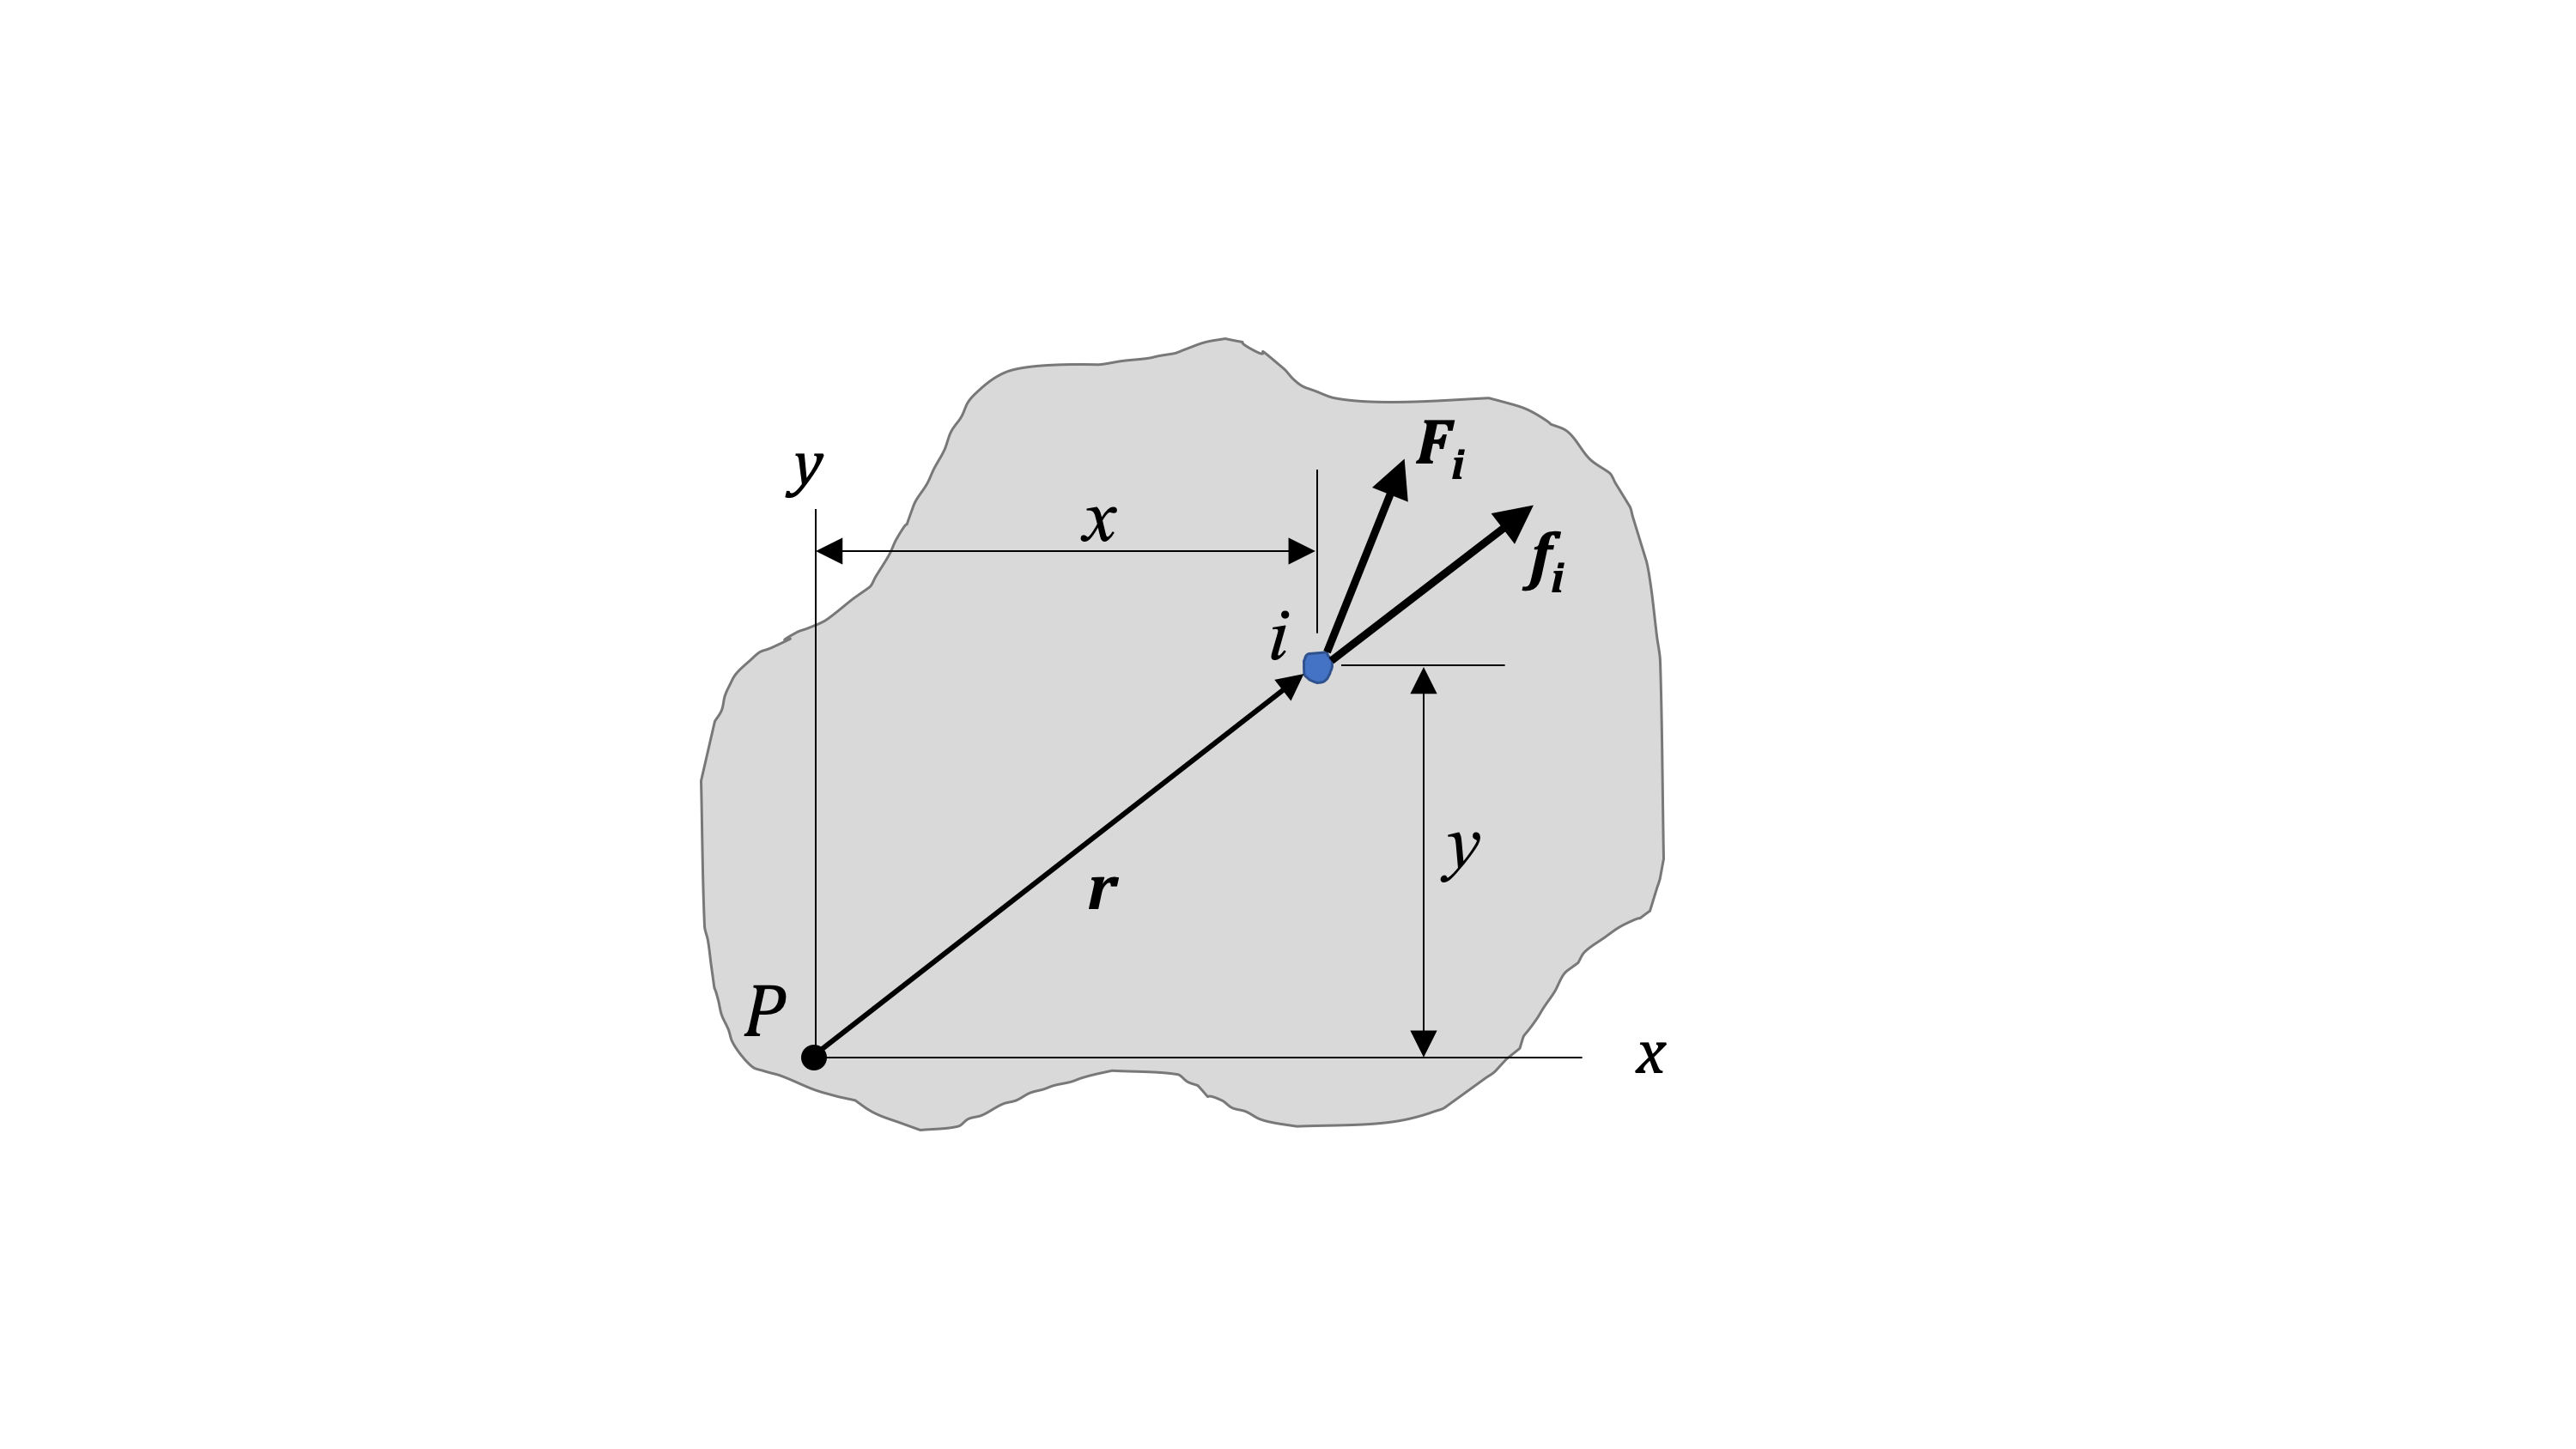
\includegraphics[trim={5cm 1cm 5cm 1cm},clip,width=0.6\textwidth, center]{Slide50} 

For each particle on the body we have:
\begin{center}
\begin{tabu} to .5\textwidth {   X[1, c]   }

$ \bm{F_1} + \bm{f_1} = m \bm{a_1} $ \\
$ \bm{F_2} + \bm{f_2} = m \bm{a_2} $\\
 $\vdots$  \\
$ \bm{F_n} + \bm{f_n} = m \bm{a_n} $ \\
\hline
$ \displaystyle \sum_i \bm{F_{external}} + \sum_i \bm{f_{internal}} = \sum m_i \bm{a_i} $
\end{tabu}
\end{center}

Looking at each term:
\begin{center}
\begin{tabu} to 1\textwidth {   X[-2.5, c] X[1, l]  X[1, l] }
$\sum_i \bm{f_{internal}} = 0$ & Rigid body assumption - otherwise the body will explode \\
& & \\
$\sum m_i \bm{a_i} = m \bm{a_G} $ & Centre of mass equation: & $\displaystyle  \bm{r_G} = \frac{\displaystyle  \sum_{i} \bm{r_i}  m_i}{\displaystyle m}$\\
& &\\
& & $\displaystyle \Rightarrow m \bm{r_G} =  \sum_{i} \bm{r_i}  m_i$\\
& &\\
& Differentiate twice: & $\displaystyle \Rightarrow m \bm{a_G} =  \sum_{i} \bm{a_i}  m_i$\\
\end{tabu}
\end{center}

Putting this together we have Newton’s second law as applied to a rigid body.  The important thing to note is where the acceleration is measured – AT THE CENTRE OF MASS.
\[ \displaystyle \sum \bm{F_{ext}} = m \bm{a_G} \]

Now, lets look at the moment balance for this body. If we take moments about point P that is on the body:

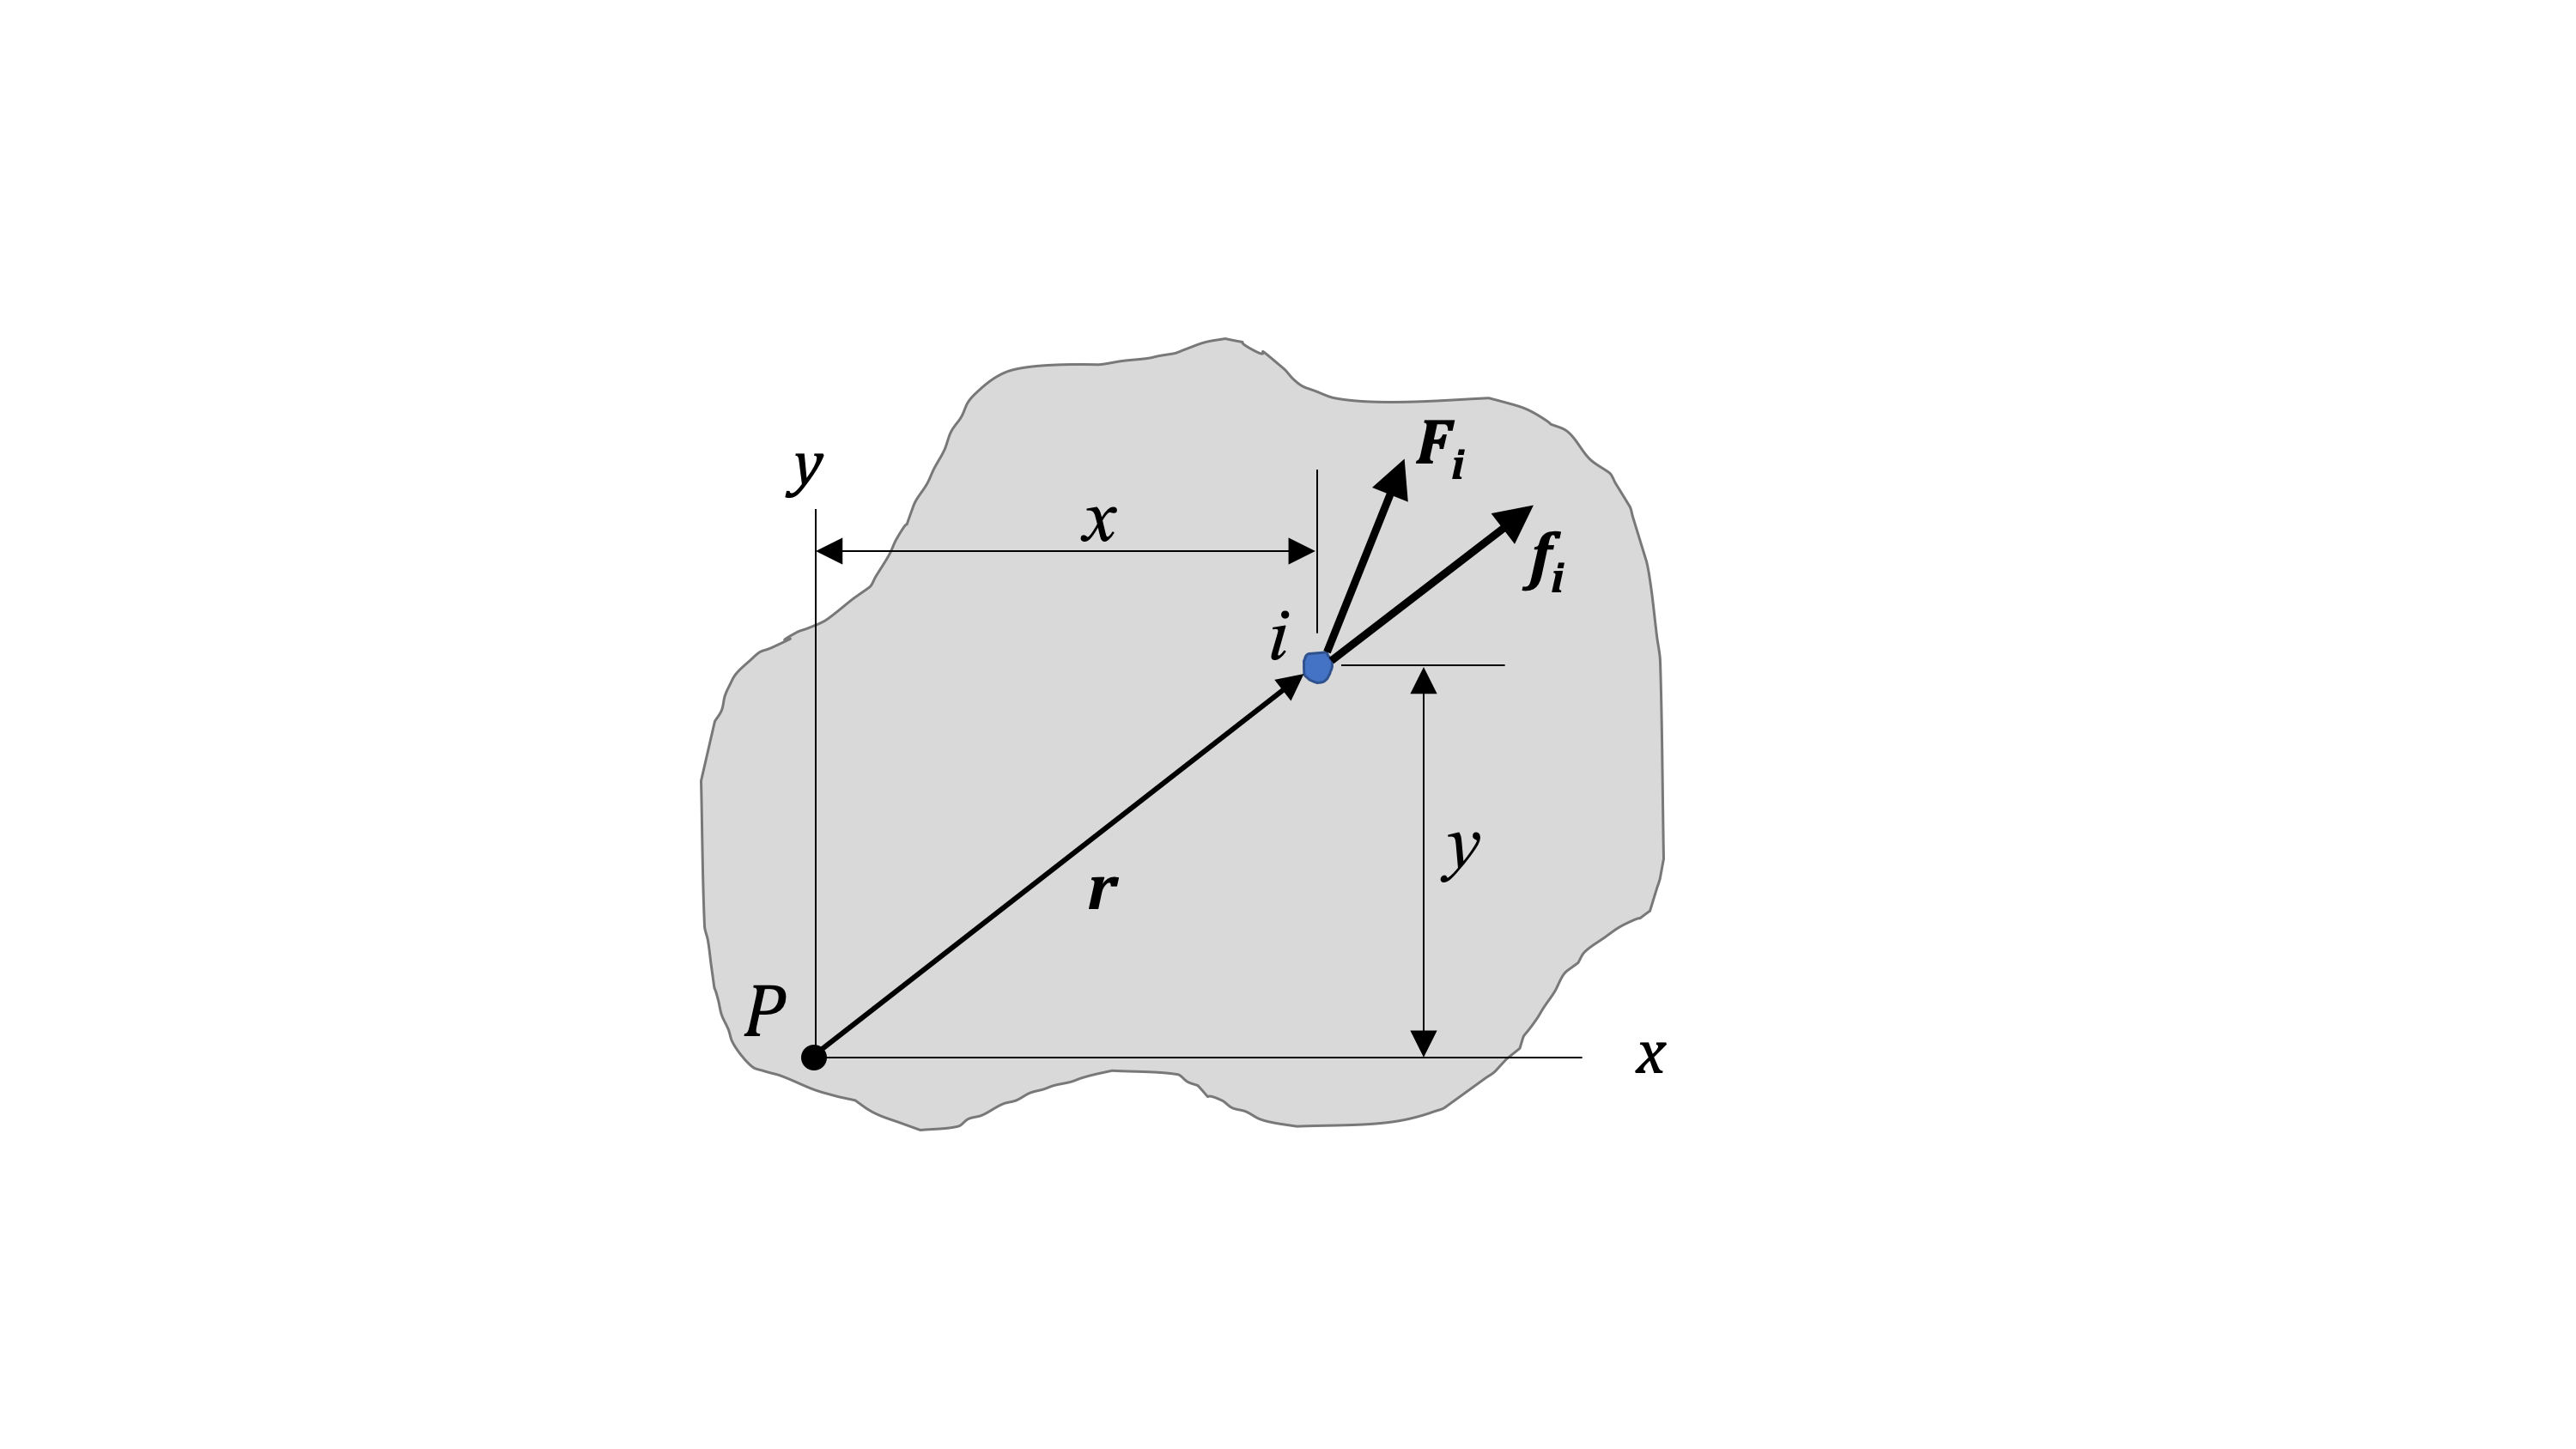
\includegraphics[trim={5cm 3cm 5cm 3cm},clip,width=0.6\textwidth, center]{Slide50} 
\[
\sum \bm{M_P} = \sum (\bm{r_i} \times \bm{F_{ext, i}}) = \sum (\bm{r_i} \times m_i \bm{a_i})
\]

Let us reference this equation in terms of G, the centre of mass of the body.
\[
\bm{r_i} = \bm{r_G} + \bm{r_{i/G}} \hspace{2 cm} \text{Note that: } \bm{r_i} =\bm{r_{i/P}} \text{ and } \bm{r_G} =\bm{r_{G/P}}
\]

\vspace*{3\baselineskip}

And we know from kinematics that at any point $\bm{a_i}$, 
\[
\bm{a_i} = \bm{a_G} + \bm{\alpha} \times \bm{r_{i/G}} - \omega^2 \bm{r_{i/G}}
\]

If we plug these last two equations into the RHS of our moment equation and simplify using the fact that, 
\[ 
\displaystyle \sum_i m_i \bm{r_{i/G}} = \sum_i m_i (\bm{r_i} - \bm{r_{G}}) = \sum_i m_i \bm{r_i} - m \bm{r_{G}} = 0
\]

\newpage

we will get:
\begin{align*}
\sum \bm{M_P} &=  \sum_i m_i (\bm{r_{G/P}} + \bm{r_{i/G}}) \times (\bm{a_G} + \bm{\alpha} \times \bm{r_{i/G}} - \omega^2 \bm{r_{i/G}}) \\
\\
&=  \sum_i m_i [ \bm{r_{G/P}} \times \bm{a_G} + \bm{r_{G/P}} \times ( \bm{\alpha} \times \bm{r_{i/G}} - \omega^2 \bm{r_{i/G}}) + \bm{r_{i/G}} \times (\bm{a_G} + \bm{\alpha} \times \bm{r_{i/G}} - \omega^2 \bm{r_{i/G}})]\\
\\
&=  \sum_i m_i (\bm{r_{G/P}} \times \bm{a_G}) + \bm{r_{G/P}} \times [ \bm{\alpha} \times (\sum_i m_i \bm{r_{i/G}}) - \omega^2 (\sum_i m_i \bm{r_{i/G}})] \\
\\
&\hspace{1cm} + (\sum_i m_i \bm{r_{i/G}}) \times \bm{a_G} + \sum_i m_i [\bm{r_{i/G}} \times (\bm{\alpha} \times \bm{r_{i/G}})] - \omega^2 \sum_i m_i (\bm{r_{i/G}} \times \bm{r_{i/G}})\\
\\
\sum \bm{M_P} &= m  \bm{r_{G/P}} \times \bm{a_G}  + \sum_i m_i \bm{r_{i/G}}^2  \bm{\alpha}\\
\end{align*}

The first part looks familiar – what we would expect if we simply multiplied our translational equation of motion by the torque arm around point $P$: $\bm{r_{G/P}} \times m \bm{a_G}$

The second part of this equation is the effect of the rotation of the entire rigid body – this is the part that relates to rotational mass – INERTIA

\[
I_G = \sum_i m_i r_{i/G}^2
\]

So finally we have an equation for the effect of moments applied to a body, about a point $P$:
\[
\sum \bm{M_P} = m  \bm{r_{G/P}} \times \bm{a_G}  + I_G \bm{\alpha}
\]

\newpage

\section{Further Results}
\begin{align*}
\sum \bm{F} &= m \bm{a_G}\\
\sum \bm{M_P} &= m  \bm{r_{G/P}} \times \bm{a_G}  + I_G \bm{\alpha}\\
\end{align*}

Applying our equation to measure the effect of Moments about at the Centre of Mass, $G$: $(\bm{r_{G/G}}=0)$
\[
\sum \bm{M_G} = I_G \bm{\alpha}
\]

For \textbf{other points on the rigid body}, we can also rewrite:
\[
\bm{a_G} = \bm{a_P} - \omega^2 \bm{r_{G/P}} + \bm{\alpha} \times \bm{r_{G/P}} 
\]

If we substitute this into our equation for $\displaystyle \sum \bm{M_P}$, we have:
\begin{align*}
\sum \bm{M_P} &= m  \bm{r_{G/P}} \times (\bm{a_P} - \omega^2 \bm{r_{G/P}} + \bm{\alpha} \times \bm{r_{G/P}} )  + I_G \bm{\alpha}\\
 &= m  \bm{r_{G/P}} \times \bm{a_P} - m  \omega^2 (\bm{r_{G/P}} \times \bm{r_{G/P}}) + m  \bm{r_{G/P}} \times (\bm{\alpha} \times \bm{r_{G/P}} )  + I_G \bm{\alpha}\\
 &= m  \bm{r_{G/P}} \times \bm{a_P} + m  r_{G/P}^2 \bm{\alpha}   + I_G \bm{\alpha}\\
 \\
\sum \bm{M_P} &= m  \bm{r_{G/P}} \times \bm{a_P}  + I_P \bm{\alpha}\\
\end{align*}

Finally, if point $P$ is PINNED (fixed to ground but body is allowed to ROTATE around $P$):
\[
\sum \bm{M_P} = I_P \bm{\alpha}
\]

\newpage

\section{Method}
\begin{enumerate}
\item Draw the free body diagram for each separate body
\item  Write Equations of Motion 
\begin{itemize}
\item $\displaystyle \sum \bm{F} = m \bm{a}$ (for planar, two equations - in plane - such as $\bm{\hat{i}}, \bm{\hat{j}}$)
\item $\displaystyle \sum \bm{M_G} = I_G \bm{\alpha}$ (for planar, one equation – out of the plane $\bm{\hat{k}}$ coordinate) \\
(can use a different moment equation if appropriate – i.e. for pinned rotation)
\end{itemize}
\item Apply KINEMATIC CONSTRAINTS
\item Solve
\end{enumerate}

\subsection{Example 1}
The pipe has a mass of $800 \, kg$ and is being towed behind a truck.  If the angle $\theta =30^{\circ}$, determine the acceleration of the truck and the tension in cable $AB$.  The coefficient of kinetic friction between the pipe and the ground is $\mu_k = 0.1$.

\includegraphics[trim={2cm 1cm 5cm 2cm},clip,width=0.5\textwidth, left]{Slide51} 

\newpage

(Example continued)
\newpage

\subsection{Example 2}
The $2 \, lb$ bottle rests on a conveyor.  If the coefficient of static friction is $\mu_s = 0.2$ determine the largest acceleration the conveyor can have without causing the bottle to slip or tip.  

\includegraphics[trim={8cm 1cm 5cm 2cm},clip,width=0.4\textwidth, left]{Slide52} 

\newpage

\subsection{Example 3}
Bar $CD$ is supported by two cables $AB$ and $CD$.  Cable $CD$ suddenly breaks.  Find the angular acceleration of the bar, and the tension in the cable $AB$ immediately after $CD$ breaks.  The mass of the bar is $10 \, kg$ and is uniformly distributed over the length of $1 \, m$.

\includegraphics[trim={1cm 4cm 1cm 1cm},clip,width=0.6\textwidth, left]{Slide53} 

\newpage
(Example continued)
\newpage

\section{Rotation About a Fixed Axis}
If a body is rotating about a fixed point (\textbf{pinned}) at O, then we can use this \textbf{kinematic constraint} to help solve the problem.  

The equations of motion for any body are:
\begin{align*}
\sum \bm{F} &= m \bm{a_G}\\
\sum \bm{M_G} &= I_G \bm{\alpha}\\
\end{align*}

\includegraphics[trim={8cm 2cm 5cm 2cm},clip,width=0.5\textwidth, center]{Slide54} 

However, for this particular case we can use kinematics to write $\bm{a_G}$ in terms of vectors parallel and perpendicular to the line between the pin and the centre of mass, $OG$: 
\[
\bm{a_G} = \bm{\alpha} \times \bm{r_{G/O}} - \omega^2 \bm{r_{G/O}}
\]
Thus:
\[
\sum \bm{F} = m \bm{\alpha} \times \bm{r_{G/O}} - m \omega^2 \bm{r_{G/O}}
\]

As well, we can use the equation for motion due to moments about a \textbf{pinned point}:
\[
\sum \bm{M_O}  = I_O \bm{\alpha}
\]

\newpage

\subsection{Example}
The cable at point $B$ supporting the $2 \, m$ by $1 \, m$ sign (mass $10 \, kg$) is suddenly broken.  Find the angular acceleration of the sign and the reaction forces at point $A$ just after the cable breaks.  

\includegraphics[trim={4cm 1cm 1cm 1cm},clip,width=0.6\textwidth, left]{Slide55} 

\vspace*{10\baselineskip}

\chapter{L12/L13/L14: General Plane Motion and Kinematic Constraints}
Readings

\section{Objective}
To apply Newton’s Second Law to \textbf{planar} rigid bodies under a number of different conditions.  To recognize and use \textbf{kinematic constraints} in order to solve these problems.  Of specific consideration are the problems involving wheels where it is not known whether the body is rolling or slipping, and this fact must be determined as part of the problem.  

\section{Review of General Methodology}
\begin{enumerate}
\item Draw the free body diagram for each separate body
\item  Write Equations of Motion 
\begin{itemize}
\item $\displaystyle \sum \bm{F} = m \bm{a}$ (for planar, two equations - in plane - such as $\bm{\hat{i}}, \bm{\hat{j}}$)
\item $\displaystyle \sum \bm{M_G} = I_G \bm{\alpha}$ (for planar, one equation – out of the plane $\bm{\hat{k}}$ coordinate) \\
(can use a different moment equation if appropriate – i.e. for pinned rotation)
\end{itemize}
\item Apply KINEMATIC CONSTRAINTS
\item Solve
\end{enumerate}

SOME IMPORTANT NOTES TO REMEMBER:  
\begin{itemize}
\item Forces must be EQUAL AND OPPOSITE on connecting links
\item Forces due to strings or cables are along the string or cable
\item Forces due to frictionless roller contact on a surface are perpendicular (normal) to the surface.
\item For surfaces with friction, friction is along the surface and opposes the CONTACT motion.  The Normal force is perpendicular to the surface.
\item In some texts (e.g. Hibbeler), a “rough surface” indicates friction present.  A “smooth surface” indicates you can neglect friction.
\end{itemize}

\subsection{Example}
A cord, $C$, is wrapped around both $10 \, kg$ disks.  If they are released from rest, determine the tension in the fixed cord, $D$.  Neglect the mass of the cord.  

\includegraphics[trim={2cm 1cm 23cm 1cm},clip,width=0.25\textwidth, left]{Slide57} 

\vspace*{10\baselineskip}

\newpage
(Example continued)
\newpage

\section{Type of Kinematic Constraints}
This is a class of problem where the type of \textbf{kinematic constraint} (in this case slipping or non-slipping) must be determined as part of the solution.  

The first step is to draw the free body diagram, including friction. It is helpful to keep in mind the direction in which friction is expected to act in considering the motion that is expected.  As shown in this figure, this can be different depending on the rest of the forces and moments involved in the FBD.

\includegraphics[trim={1cm 7cm 6cm 3cm},clip,width=0.8\textwidth, left]{Slide58} 

The next step is to write the equations of motion related to the free body diagram.  Considering the free body diagram on the right, we can write the equations of motion as:
\vspace*{8\baselineskip}

Given W and M, these three equations have four unknowns:
\vspace*{6\baselineskip}

In the case that the wheel is rolling without slipping the force of friction, 
\[
f \leq \mu_s N
\]

Where $ \mu_s$ is the static coefficient of friction.  For rolling without slipping, we know that the velocity of the bottom of the wheel is the same as the velocity of contact surface (relative velocity is zero).  We can use this kinematic constraint to specify the relationship between the acceleration of the center of the wheel and the angular acceleration of the wheel.  

\[
\bm{a_{G_x}} = \bm{\alpha} \times \bm{r}
\]

This fourth equation allows the problem to be solved provided that $f \leq \mu_s N$. 

\vspace*{11\baselineskip}

What if the solutions yields $f > \mu_s N$? Then slipping occurs, and our kinematic constraint does not hold.  In this case we use $f = \mu_k N$ as our fourth equation and then we can solve the problem.  
 
\vspace*{5\baselineskip} 
 
\section{Method}
\begin{enumerate}
\item Draw the free body diagram for each separate body
\item  Write Equations of Motion 
\begin{itemize}
\item $\displaystyle \sum \bm{F} = m \bm{a}$ (for planar, two equations - in plane - such as $\bm{\hat{i}}, \bm{\hat{j}}$)
\item $\displaystyle \sum \bm{M_G} = I_G \bm{\alpha}$ (for planar, one equation – out of the plane $\bm{\hat{k}}$ coordinate) \\
(can use a different moment equation if appropriate – i.e. for pinned rotation)
\end{itemize}
\item Apply KINEMATIC CONSTRAINTS. First assume no slipping $f \leq \mu_s N$ and solve. Check the no-slipping assumption.  If this yields $f > \mu_s N$ then use $f = \mu_k N$ as the extra relationship and solve the problem.
\end{enumerate}

Can I skip a step and use $f = \mu_k N$ right away?  NO!  You cannot make the sliding case assumption without checking the non-sliding condition first.

NOTE:  Typically $ \mu_k < \mu_s$

The determination of the type of kinematic constraint (sliding/not sliding) can also occur in problems such as this one:  

\subsection{Example}
Find the angular acceleration of the bar and the linear acceleration of point $G$, immediately after line $AB$ is cut.  Take $m = 10 \, kg$, $l=2 \, m$, $\mu_s=0.5$, $\mu_k=0.4$, $g=9.81 \, m/s^2$, and $\theta = 45^{\circ}$.  

\includegraphics[trim={0cm 1cm 22cm 1cm},clip,width=0.3\textwidth, left]{Slide59} 

\newpage

(Example continued)

\newpage

(Example continued)

\newpage

\section{Review Question}
The uniform bar $AB$, mass $m$ is attached to the hoop of negligible mass.  The hoop is released from rest in the position shown.  What is the minimum coefficient of friction for the hoop to roll without slipping – in this case give the force of friction acting on the hoop, as well as the normal force at $C$.  Also find the moment acting on the bar applied by the hoop at point $B$.

\includegraphics[trim={0cm 1cm 20cm 2cm},clip,width=0.3\textwidth, left]{Slide60} 


\newpage

\vspace*{32\baselineskip}

REVIEW: Types of contacts related to the forces and moments they can support. 

 \includegraphics[trim={1cm 1cm 14cm 7cm},clip,width=0.5\textwidth, left]{Slide61} 

\newpage

(Example continued)

\chapter{L15/L16/L17: Work and Energy}
Readings
\section{Objective}
To use the concepts of Work and Energy in an Equilibrium Equation to solve MOTION (dynamics) problems.

\section{Key Concepts}
STATE EQUATIONS
Newton’s Second Law equations are INSTANTANEOUS equations
“At this instant” find $\alpha$, $a$  - Must INTEGRATE to find position, velocity at a LATER time (state).


\vspace*{8\baselineskip}

Work and Energy equations are STATE EQUATIONS

 \includegraphics[trim={0cm 2cm 0cm 1cm},clip,width=0.8\textwidth, center]{Slide63}


Start with ENERGY of system at STATE 1 (time $t_1$). Add or subtract WORK. Yields ENERGY of system at STATE 2 (time $t_2$).

\section{Work}
Energy is a measure of the \textbf{stored ability to do work}.  Work and Energy are both measured in the same units – the SI units for work and energy are Joules.  $1 \, Joule = 1 \, N$-$m$.  Other units include $ft$-$lb$, $kcal$, $BTU$, $KWh$, and $ergs$.  

Right away we see that work and energy relate to force and distance.  And in fact, work done, $U$, by a force, $F$, can be measured as force applied over distance, i.e.:
\begin{align*}
dU &= \bm{F} \cdot \bm{dr}\\
U &= \int_S F \cos \theta ds\\
\end{align*}

Here, force and distance are both vector quantities and $\theta$ is the angle between these vectors.  For a constant force applied at a constant angle along a distance, $s_2 - s_1$, we have
\[U = F \cos \theta (s_2 - s_1) \]

Work  can also  be done by a torque. In this case, work is the torque applied over an angle: 
\[
dU = \bm{M} \cdot \bm{d \theta}
\]

For planar motion, since angle and torque are both about the same axis (the axis perpendicular to the plane), for constant torque we can write

\[
U = M(\theta_2 - \theta_1)
\]

(NOTE:  $\theta$ is in radians!)

\textbf{Work is a scalar value}.  If it is positive, this means that work is being done by the force being considered.  If it is negative then work is being done against the force being considered.  Friction, for example, never does positive work since it always opposes motion (does negative work).  Thus, friction is always associated with a loss of energy (loss of the stored ability to do work).

\subsection{Examples - Work Done by Various Forces}

 \includegraphics[trim={0cm 0cm 18cm 1cm},clip,width=0.4\textwidth, left]{Slide64}

\newpage

 \includegraphics[trim={1cm 6cm 11.5cm 0cm},clip,width=0.6\textwidth, left]{Slide65}

Recall, (Hooke’s Law) $k$ is the spring constant (in SI units $k$ is in $N/m$). 

 \includegraphics[trim={0cm 5cm 19cm 1cm},clip,width=0.4\textwidth, left]{Slide66}


\section{Power}
Power is the rate at which work is done.  The higher the power the faster work is done.  

\[
\displaystyle P = \frac{dU}{dt}
\]

Since:
\[
dU = \bm{F} \cdot \bm{ds}
\]
\[
\displaystyle P = \frac{dU}{dt} = \bm{F} \cdot \frac{d\bm{s}}{dt} = \bm{F} \cdot \bm{v}
\]

Power is also a SCALAR Value.  SI units for power are Watts. $1 \, W = 1 \, J/s = 1 \, N$-$m/s$.

\subsection{Example - Power}
Find the power required to move the block of mass $2 \, kg$ up the $45^{\circ}$ ramp with a constant speed $2 \, m/s$, assuming the coefficient of friction between the block and the ramp is $\mu_k = 0.3$, and $\theta =15^{\circ}$. 

 \includegraphics[trim={0cm 0cm 18cm 1cm},clip,width=0.4\textwidth, left]{Slide64}

\newpage
(Example continued)
\newpage

\section{Forces That Don't Do Work}
Normal Forces (perpendicular to motion, therefore $\bm{N} \cdot d \bm{s}=0$)

\vspace*{5\baselineskip}

Forces with NO MOTION

\vspace*{5\baselineskip}

Internal Forces (equal and opposite)

\vspace*{5\baselineskip}

\section{Mechanical Energy}
Energy is the stored ability to do work.  Mechanical Energy refers to energy stored by a mechanism. 

Mechanical Energy can be stored as Potential Energy (P.E.), denoted with the symbol, $V$, or Kinetic Energy (K.E.), denoted with the symbol $T$.

\section{Kinetic Energy}
Kinetic Energy is energy stored in motion.  Any body that is translating and or rotating has kinetic energy.  In the absence of energy input to the system, this energy can be:
\begin{itemize}
\item Maintained by the body maintaining it’s motion (if there are no losses of energy due to friction)
\item Dissipated – due to work done against friction
\item Used to do (useful) work
\item Transferred and stored as potential energy (e.g. stored in a mechanical or electrical storage component – spring storage, gravitational storage, battery storage)
\end{itemize}

For a body that is only translating, Kinetic Energy is computed as:
\[
T = \frac{1}{2} m v_G^2
\]

where $v_G$ is the velocity of the centre of mass of the body.  For a body that is only rotating, Kinetic Energy is computed as:
\[
T = \frac{1}{2} I_G \omega^2
\]

where $I_G$ is the mass moment of inertia of the body around its \textbf{centre of mass}.  THE REFERENCE TO CENTRE OF MASS IS IMPORTANT (inertia is different around different axes!).

For a body that is both translating and rotating, the Kinetic Energy is the sum of both rotational and translational energies:
\[
T = \frac{1}{2} m v_G^2 + \frac{1}{2} I_G \omega^2
\]

\subsection{Example 1 - Kinetic Energy}
Find the kinetic energy of a wheel rolling without slipping:

 \includegraphics[trim={0cm 1cm 20cm 1cm},clip,width=0.35\textwidth, left]{Slide67}

\newpage

Note:  for a body rotating around a point that is not moving
(around a point $P$ – a PIN or the ICZV):
\begin{align*}
T &= \frac{1}{2} m v_G^2 + \frac{1}{2} I_G \omega^2 = \frac{1}{2} ( m (\omega r_{G/P})^2 +  I_G \omega^2) =  \frac{1}{2} ( m  r_{G/P}^2 +  I_G) \omega^2\\
T &=  \frac{1}{2} I_P \omega^2 \\
\end{align*}
USE WITH CAUTION – ONLY VALID AROUND A PIN OR ICZV!

\subsection{Example 2 - Kinetic Energy}
Find the kinetic energy of the mechanism shown, use $\rho_{bar}=0.5 \, lb/in$.

 \includegraphics[trim={0cm 1cm 19cm 0cm},clip,width=0.4\textwidth, left]{Slide68}
\newpage


\section{Potential Energy}
The amount of potential energy stored is dependant on location \textbf{with respect to a datum}.  Change in potential energy depends only on the change of position, and is \textbf{independent of path}.

Potential energy can be stored as \textbf{gravitational potential energy}:
\[
V_g = mgy_G
\]
where m is the mass of the body, $g$ is the acceleration due to gravity and $y_G$ is the distance up measured from a datum to the \textbf{centre of mass} of the body.

 \includegraphics[trim={0cm 1cm 19cm 1cm},clip,width=0.4\textwidth, left]{Slide69}

In the figure, the body of mass, $m$, has potential energy:
\[
V_{g_1} = mgh
\]

at the top point, and 
\[
V_{g_2} = -mgd
\]

at the bottom point (i.e. it has negative potential energy with respect to some arbitrary datum.  The change in potential energy as the body falls between top and bottom is: 
\[
V_{g_2} - V_{g_1}= -mgd -mgh = -mg(d+h)
\]

That is the body has lost potential energy.  If the body is moved up from the bottom to the top, they it is said to have gained potential energy:
\[
V_{g_1} - V_{g_2}= mgh -(-mgd) = mg(d+h)
\]

Note that, an increase in stored gravitational potential energy results from work being done against the force of gravity (gravity did negative work – i.e. something else did positive work to lift the mass up).  
\begin{align*}
U_{g(1 \rightarrow 2)} &= \bm{W} \cdot \Delta \bm{r_G}\\
&= -(mg) \bm{\hat{j}} \cdot (h-(-d)) \bm{\hat{j}}\\
&= -mg(h+d)\\
\end{align*}

Potential Energy can also be stored in a spring.  Again we set a datum, this time, the unstretched length of the spring, $s=0$.  

 \includegraphics[trim={0cm 1cm 19cm 1cm},clip,width=0.4\textwidth, left]{Slide70}

As the spring is stretched or compressed, work is done against the spring, and energy is stored in the spring.  

The stored potential is:
\[
V_s = \frac{1}{2} k s^2
\]

(recall $k$ is the spring constant and s is measured from unstretched length.) Note that, the potential energy in a spring is always greater than zero.  However, a spring can gain or lose potential energy.  

When a spring does work, it loses potential:
\[
\displaystyle U_{1 \rightarrow 2} = \int \bm{F} \cdot d \bm{s} = \int_{s_1}^{s_2} -kx dx = - \frac{1}{2} k(s_1^2 - s_2^2)
\]

A torsional spring works along the same principle except that instead of measuring linear displacement, $s$¸ from the unstretched length, we measure angular displacement from the untwisted state.  The displacement is measured in radians, and the spring constant is measured in units of force $x$ distance (SI units $N$-$m$).
\[
V_s = \frac{1}{2} k_{\theta} \theta^2
\]

\subsection{Example - Potential Energy}
Find the change in potential energy of the mechanical system from point $A$ to point $C$.  The collar has a weight of $5 \, lbs$.  The unstretched length of the spring is $12 \, inches$.  

 \includegraphics[trim={1cm 0cm 18cm 1cm},clip,width=0.35\textwidth, left]{Slide71}

\newpage

\section{Conservative Forces}
Potential Energy is related to Conservative Forces.  These are forces for which the work done is \textbf{independent of path} – depends only on the starting and ending points. 

Compare with friction for which the (negative) work done is \textbf{path dependant}.  

Potential Energy and Conservative Forces are related in the through the gradient operator, “del”:
\[
\displaystyle \bm{F} = - \nabla V = - \left( \frac{\partial}{\partial x} \bm{\hat{i}} + \frac{\partial}{\partial y} \bm{\hat{j}} + \frac{\partial}{\partial z} \bm{\hat{k}} \right) V
\]

Thus, for gravitational potential (assuming $y$  is “up”) we see
\begin{align*}
\displaystyle \bm{F_g} &= - \nabla V_g = - \left( \frac{\partial}{\partial x} \bm{\hat{i}} + \frac{\partial}{\partial y} \bm{\hat{j}} + \frac{\partial}{\partial z} \bm{\hat{k}} \right) mgy_G\\
&= \frac{\partial}{\partial y} (mgy_G) \bm{\hat{j}}\\
&=-mg \bm{\hat{j}}\\
\end{align*}

For spring potential assuming the spring stretches along $x$, where $x=0$ at the unstretched length:
\begin{align*}
\displaystyle \bm{F_s} &= - \nabla V_s = - \left( \frac{\partial}{\partial x} \bm{\hat{i}} + \frac{\partial}{\partial y} \bm{\hat{j}} + \frac{\partial}{\partial z} \bm{\hat{k}} \right) \frac{1}{2} k x^2\\
&= - \frac{\partial}{\partial x} \left( \frac{1}{2} k x^2 \right) \bm{\hat{i}}\\
&=-kx \bm{\hat{i}}\\
\end{align*}

\section{Principle of Work and Energy}
We can bring all of these energy terms together into the following relationship for a system: 
\[
T_1 + V_1 + \sum_{non-conservative \,work}U_{1 \rightarrow 2} = T_2 + V_2
\]

\vspace*{2\baselineskip}
In other words, in state 1, the system starts out with a quantity of potential and kinetic energy (that can be added together).  As the system moves from state 1 to state 2, if no work is added or subtracted from the system (input from a motor, or losses from friction) then the total quantity of potential and kinetic energy at state 2 will be the same (although their relative amounts may change).  

However, in most mechanical systems, there will be “non-conservative” losses due to friction.  Thus, the total amount of kinetic and potential energy at state 2 will be reduced.  

\vspace*{16\baselineskip}


\section{Method}
\begin{enumerate}
\item Identify all bodies in the system
\item \textbf{For each body}, 
\begin{itemize}
\item Draw the free body diagram to identify:
\begin{itemize}
\item Conservative forces (related to changes in \textbf{potential energy – path independent changes in energy})
\item Non-conservative forces (related to the addition or subtraction of energy in the form of \textbf{work})
\end{itemize}
\item Consider Potential Energy
\begin{itemize}
\item Draw two diagrams showing the body located at its initial and final state.
\item Identify a datum and find the potential energy at state 1 and state 2 for each conservative force.  Gravitational potential energy ($V_G =mgh$) can be positive or negative.  Spring potential energy ($V_s = \frac{1}{2} k s^2$) is always positive.
\item Potential Energy at each state is the SUM of the potential energy related to all conservative forces in the system.
\end{itemize}
\item Consider Work by non-conservative forces over the path.  Between state 1 and state 2, integrate all sources of work related to non-conservative forces:
\begin{itemize}
\item $dU = \bm{F} \cdot d \bm{r}$
\item $dU = \bm{M} \cdot d \bm{\theta}$
\item Work done from state 1 to state 2 can be positive or negative.  Friction always does negative work.  
\end{itemize}
\item Consider Kinetic Energy at each state: $T = \frac{1}{2} m v_G^2 + \frac{1}{2} I_G \omega^2$
\item Principle of Work and Energy: $T_1 + V_1 + \sum_{non-conservative \,work}U_{1 \rightarrow 2} = T_2 + V_2$
\end{itemize}
\end{enumerate}

\subsection{Example 1 – Principle of Work and Energy}
The $5 \, lb$ collar is released from rest at $A$ and travels along a smooth guide.  Find its speed when it reaches point $C$.  The unstretched length of the spring is $12 \, inches$.  How would the solution change if there was friction between the collar and the guide?

 \includegraphics[trim={1cm 0cm 18cm 1cm},clip,width=0.35\textwidth, left]{Slide71}

\vspace*{10\baselineskip}
\newpage

\subsection{Example 2 – Principle of Work and Energy}

The uniform bar has mass $m$ and length $l$.  If it is released from rest when $\theta = 0^{\circ}$, determine the angle $\theta$ at which it first begins to slip.  The coefficient of static friction is $\mu_s = 0.3$.  

\includegraphics[trim={0cm 2cm 18cm 6cm},clip,width=0.4\textwidth, left]{Slide72}

\vspace*{10\baselineskip}
\newpage

(Example continued)

\newpage

\section{Summary}
\begin{center}
\begin{tabu} to 1\textwidth {  | X[1, l]  | X[1, c] | X[1, l] | }
\hline
 & & \\
Work & $dU = \bm{F} \cdot d \bm{r}$
 $dU = \bm{M} \cdot d \bm{\theta}$ & Force along a path, Moment through an angle\\
& & \\
\hline
& & \\
Kinetic Energy & $T = \frac{1}{2} m v_G^2 + \frac{1}{2} I_G \omega^2$ & Energy stored as motion \\
 & & \\
& $T =  \frac{1}{2} I_O \omega^2$ if pinned at $O$ & \\
& & \\
\hline
& & \\
Potential Energy & & Path independent change of the stored ability for a conservative force to do work\\
& & \\
& $V_G =mgh$ & Gravitational potential energy can be positive or negative\\
& & \\
& $V_s = \frac{1}{2} k s^2$ & Spring potential energy is always positive\\
& & \\
\hline
& \multicolumn2{|c|}{ } \\
Principle of Work and Energy& \multicolumn2{|c|}{$T_1 + V_1 + \sum_{non-conservative \,work}U_{1 \rightarrow 2} = T_2 + V_2$} \\
& \multicolumn2{|c|}{ } \\
\hline
\end{tabu}
\end{center}

If we compare this to Newton’s Second Law Equation (for a point mass), $\bm{F} = m \bm{a}$, and we consider $F$ to be a force which we integrate between two states, we see: 
\[
\displaystyle \sum_{all \, work} U_{1 \rightarrow 2} = \int \bm{F} \cdot d \bm{s} = \int m \bm{a} \cdot d \bm{s} = \int m \frac{d \bm{v}}{dt} \cdot d \bm{s} = \int m \bm{v} \cdot d \bm{v} = \frac{1}{2} m(v_2^2 - v_1^2) = T_2 - T_1
\]

In other words, the Principle of Work and Energy is the same as integrating Newton’s Second Law over the motion from state 1 to state 2.  

\chapter{L18: Free Undamped Vibrations}
Readings

\section{Objective}
Introduce Single Degree of Freedom Vibration of a rigid body. 
\begin{itemize}
\item Define terminology
\item Establish model of single degree of freedom vibrations using Newton’s Second Law
\item Show examples in mechanical systems
\end{itemize}

\section{Free Vibration}
A vibrating mechanical system is a system that exchanges kinetic and potential energy.  Therefore it must have:
\begin{enumerate}
\item Potential field (i.e., an element that can store and release potential energy)
\item Inertia (mass, or moment of inertia) – an element that can have kinetic energy
\end{enumerate}

In the real world, mechanical systems also have energy losses – through friction and often (intentionally) through energy absorbing devices or materials called “dampers”.  To start we will ignore these losses and look at a simple vibrating mass-spring system, and some related models

\vspace*{10\baselineskip}

Consider the mass attached to a spring, moving along with no friction.

\includegraphics[trim={1cm 1cm 2cm 3cm},clip,width=0.6\textwidth, left]{Slide74}

We set our datum for the system where the spring is unstretched.  Then we draw the free body diagram of the block:

\vspace*{8\baselineskip}

And write the equations of motion

\vspace*{4\baselineskip}

We can express the spring force, using Hooke’s Law:
\vspace*{5\baselineskip}

So the equation of motion for the free motion – free vibration – of the system is a Homogeneous, second order, differential equation.
\[
m \ddot{x} (t) + kx(t) = 0
\]

The solution for this type of motion – simple harmonic motion – is of the form:
\begin{align*}
x(t) &= A \sin (\omega t) + B \cos (\omega t)\\
\dot{x}(t) &= A \omega \cos (\omega t) - B \omega \sin (\omega t)\\
\ddot{x}(t) &= -A \omega^2 \sin (\omega t) - B \omega^2 \cos (\omega t) = - \omega^2 x(t)\\
\end{align*}

Substituting back into the differential equation we get:
\[
m (- \omega^2 x(t)) + kx(t) = 0
\]

$\omega$ that satisfies this equation is: $\displaystyle \omega_n = \sqrt{\frac{k}{m}}$

$\omega_n$ is the \textbf{angular natural frequency} of the system, measured in $radians/second$.  For example, $\omega_n = 2\pi$ implies that the system repeats itself every second.  

$\displaystyle f = \frac{\omega_n}{2\pi}$ is the frequency of the system in $Hertz = cycles/second=s^{-1}$. 

$\displaystyle T = \frac{1}{f} = \frac{2\pi}{\omega_n}$ is the time to complete one vibration cycle. 

\includegraphics[trim={0cm 0cm 0cm 0cm},clip,width=0.6\textwidth, center]{Slide75}

Another form of the solution:  $x = C \sin (\omega_n t + \phi)$

\textbf{Natural frequency} of a system depends only on its physical properties – for spring type vibration it depends on the system inertia (mass) and stiffness.

\begin{center}
\begin{tabu} to 1\textwidth {  | X[1, c]  | X[1, l] | }
\hline
& \\
& Increasing stiffness increases frequency of vibration\\
$\displaystyle \omega_n = \sqrt{\frac{k}{m}}$ & \\
& Increasing mass decreases frequency of vibration\\
& \\
\hline
\end{tabu}
\end{center}

\section{Initial Conditions}
\[
x(t) = A \sin (\omega_n t) + B \cos (\omega_n t)
\]

Assume at $t = 0$, $x(0) = x_0$ and $\dot{x}(0) = v_0$:
\[
x_0 = A \sin (0) + B \cos (0) \, \Rightarrow \, B = x_0
\]
\[
v_0 = \omega(A \cos (0) - B \sin (0)) \, \Rightarrow \, A = \frac{v_0}{\omega_n}
\]

Thus:
\[
x(t) = \frac{v_0}{\omega_n} \sin (\omega_n t) + x_0 \cos (\omega_n t)
\]

To see the relationship between these constants we can construct a right triangle:

\includegraphics[trim={2cm 0cm 2cm 1cm},clip,width=0.6\textwidth, center]{Slide76}

\vspace*{2\baselineskip}

$C = \sqrt{A^2 + B^2}$ is the \textbf{amplitude} of the system.  $\phi$ is the \textbf{phase angle}.  These values are related to the initial conditions and also to the natural frequency (for non-zero $v_0$).  

\begin{center}
\begin{tabu} to 1\textwidth {   X[1, c]  X[1, C]  X[1, C]  }
$A = C \cos (\phi)$ & & $x(t) = C \cos (\phi) \sin (\omega_n t) + C \sin (\phi) \cos (\omega_n t)$ \\
& $\Rightarrow$ & \\
$B = C \sin (\phi)$ & & $x(t) = C \sin (\omega_n t + \phi)$\\
\end{tabu}
\end{center}

\includegraphics[trim={0cm 0cm 0cm 0cm},clip,width=0.8\textwidth, center]{Slide75}

\begin{align*}
x(t) &= C \sin (\omega_n t+ \phi)\\
\dot{x}(t) &= C \omega_n \cos (\omega_n t+ \phi) = C  \omega_n \left( \omega_n t + \phi + \frac{\pi}{2} \right)\\
\ddot{x}(t) &= - C \omega_n^2 \sin (\omega_n t+ \phi) = C  \omega_n \left( \omega_n t + \phi + \pi \right)\\
\end{align*}

\textbf{Process:}
\vspace*{20\baselineskip}


\subsection{Example 1 - Torsional Shaft Vibration}


\includegraphics[trim={6cm 0cm 5cm 0cm},clip,width=0.5\textwidth, left]{Slide77}

\vspace*{10\baselineskip}
\newpage

\subsection{Example 2 - Swinging Pendulum (small $\theta$)}

\includegraphics[trim={2cm 1cm 20cm 1cm},clip,width=0.35\textwidth, left]{Slide78}
\vspace*{10\baselineskip}
\newpage

\section{Simple Harmonic Motion Solution using Euler's Formula}
Equation of motion:
\begin{equation} \label{eq:11.4}
m \ddot{x} (t) + kx(t) = 0
\end{equation}

Propose solution of the form:  $x=ae^{rt}$

Substitute back into (\ref{eq:11.4}) and cancel out $e^{rt}$ terms.
\[
mr^2+k=0 \, \Rightarrow \, r= \pm \sqrt{- \frac{k}{m}} = \pm \omega_n i
\]
where $i$ is the imaginary number, $i = \sqrt{-1}$.

So our solution is of the form
\[
x(t) = a_1 e^{i \omega_n t} + a_2 e^{-i \omega_n t}
\]

\textbf{Euler's formulae:}
\[
e^{i \omega_n t} = \cos ( \omega_n t) + i \sin ( \omega_n t)
\]
\[
e^{-i \omega_n t} = \cos ( \omega_n t) - i \sin ( \omega_n t)
\]

\includegraphics[trim={2cm 3cm 18cm 1cm},clip,width=0.25\textwidth, center]{Slide79}

Since $x(t)$ is REAL, $a_1$ and $a_2$ must be complex conjugate numbers.
\begin{align*}
x(t) &= ( a_1+a_2) \cos (\omega_n t) + (a_1 - a_2) i \sin (\omega_n t)\\
&= B \cos (\omega_n t) + A \sin (\omega_n t)\\
&= C\sin (\omega_n t + \phi)\\
\end{align*}

Where:
\[
a_1 = \frac{B - Ai}{2} \, , \, a_2 = \frac{B + Ai}{2}
\]

\newpage

\section{Summary}
For undamped, single degree of freedom vibration, the form of the equation of motion is:
\[
m \ddot{x} (t) + kx(t) = 0
\]
\vspace*{2\baselineskip}

$\displaystyle \omega_n = \sqrt{\frac{k}{m}}$ is the (angular) natural frequency of the system.  Natural frequency depends on physical system parameters and is independent of initial conditions. 

\includegraphics[trim={0cm 0cm 0cm 0cm},clip,width=0.7\textwidth, center]{Slide75}

Initial conditions specify the amplitude of vibration, $C$, and the phase angle, $\phi$.  

For $x(0) = x_0$ and $\dot{x} (0) = v_0$:
\[
\displaystyle C=\sqrt{\left( \frac{v_0}{\omega_n} \right)^2 + x_0^2} \, , \, \tan \phi  = \frac{\omega_n x_0}{v_0}
\]

\includegraphics[trim={2cm 0cm 2cm 1cm},clip,width=0.6\textwidth, center]{Slide76}

\newpage

\subsection{Example}
A cord, running over a pulley (mass 7.5 kg, radius 0.25 m), connects a spring (k = 3500 N/m) with a hanging mass (5 kg). What is the natural period of vibration of the system?

\includegraphics[trim={0cm 0cm 14cm 1cm},clip,width=0.4\textwidth, left]{Slide80}

\chapter{L19: \sout{Modelling Using Energy Methods} (NOT 2020W)}
Reading

\section{Objective}
To use conservation of energy principles to generate the equation of motion for a vibrating system.  

\section{Conservation of Energy}

\begin{minipage}{0.35\textwidth}
\includegraphics[trim={0cm 0cm 20cm 0cm},clip,width=1\textwidth, left]{Slide117}
\end{minipage}
\begin{minipage}{0.65\textwidth}
Consider the mass spring system shown.  Assume the mass is displaced along the $x$ direction. 

The potential energy due to the spring is:  $V_s = \frac{1}{2}k(\Delta + x)^2$

Setting our datum at $x=0$, with $x$ pointing down, the potential energy due to gravity is: 

\[V_g = -mgx\]

Total potential energy is:
\[
V = V_g + V_s = \frac{1}{2} k (\Delta + x)^2 - mgx
\]

Once the system is moving, the kinetic energy of the system depends on the velocity of the mass:

\[
T = \frac{1}{2}mv^2 = \frac{1}{2}m \dot{x}^2
\]
\end{minipage}


Conservation of energy tells us that for all time (as long as there is no external input of energy, and no energy losses):
\[
T+V = constant
\]

\[
\Rightarrow \displaystyle \frac{1}{2} m \dot{x}^2 + \frac{1}{2} k (\Delta + x)^2 - mgx = constant
\]

This equation shows that at any state: $(x, \dot{x})$, the energy in the system is traded off between potential energy (related to $x$) and kinetic energy (related to $v= \dot{x}$).  But it does not tell us the time-domain story of what the system is doing.

Differentiating this equation yields:

\[
\frac{d}{dt} : \, m \dot{x} \ddot{x} + k(\Delta + x) \dot{x} - mg \dot{x} = 0
\]

Dividing out $\dot{x}$ (i.e. if the system isn’t moving $(\dot{x}=0)$ then there isn’t much to talk about …). 

\[
m \ddot{x} + k(\Delta +x) - mg = 0
\]

If we look at the Equilibrium position of the system, we see that:

\begin{minipage}{0.35\textwidth}
\includegraphics[trim={0cm 0cm 22cm 0cm},clip,width=1\textwidth, left]{Slide118}
\end{minipage}
\begin{minipage}{0.65\textwidth}

$mg-k\Delta = 0$

\vspace*{3\baselineskip}

$m \ddot{x} + kx = 0$     \hspace{1cm}    our old friend!  

\end{minipage}

\section{Observations}
Energy methods can be used to model \textbf{conservative systems} (no friction or damping) and to compute the natural frequency of more complex systems.  

Energy methods allow computation of the equation of motion of multi-component systems without being concerned about internal forces (which don’t do work).  With Second-Law methods, would have to draw FBD’s and write equations of motion for each system.  

\newpage

\subsection{Example 1}
Use the Energy method to find the natural frequency of a ball, mass $m$, radius $r$, rolling on a circular surface of radius $R$.  

\includegraphics[trim={0cm 2cm 16cm 6cm},clip,width=0.5\textwidth, left]{Slide119}

\vspace*{6\baselineskip}


\newpage

\subsection{Example 2}
What is the natural frequency of a kayak?  How is its natural frequency affected by the kayak's shape?

\includegraphics[trim={0cm 3cm 8cm 5cm},clip,width=0.65\textwidth, left]{Slide120}

\vspace*{6\baselineskip}

\chapter{L20: Harmonic Forced Undamped Vibration}
Readings

\section{Objectives}
\begin{itemize}
\item To model the behaviour of undamped systems under harmonic excitation. 
\item Identify the complementary, particular, and general solution of the equation of motion for the system.
\item Observe how the amplitude of motion changes as a function of the relationship between the forced frequency and the system natural frequency.  
\item Observe the phenomena of beats, and resonance. 
\end{itemize}

\section{Mass Spring Model}
\includegraphics[trim={1cm 1cm 2cm 4cm},clip,width=0.5\textwidth, left]{Slide82}

If we write the equations of motion for the system:
\[
\sum F_x = ma
\]
\[
-kx + F_0 \sin \omega_0 t = m \ddot{x}
\]
\[
\Rightarrow m \ddot{x} + kx = F_0 \sin \omega_0t
\]

The \textbf{general solution} of this equation is composed of the superposition of the \textbf{complementary solution} and the \textbf{particular solution}.  

For the complementary solution set $RHS = 0$.
\[ 
x_c = C \sin (\omega_n t + \phi)
\]
\[ \text{where} \, \omega_n = \sqrt{\frac{k}{m}}
\]

For the particular solution, since the forcing function is periodic, assume a similar periodic solution:
\begin{align*}
x_p &= D \sin (\omega_0 t)\\
\ddot{x}_p &= -\omega_0^2 D \sin (\omega_0 t)\\
\end{align*}

Substituting this back into our equation of motion:
\[
-m \omega_0^2 D \sin (\omega_0 t) + k D \sin (\omega_0 t) = F_0 \sin ( \omega_0 t)
\]

We can then solve for D, as:
\[
\displaystyle D = \frac{\displaystyle \frac{F_0}{k}}{1- \left( \displaystyle \frac{\omega_0}{\omega_n} \right)^2}
\]

Thus, the particular solution is:
\[
x_p = \frac{\displaystyle \frac{F_0}{k}}{1- \left( \displaystyle \frac{\omega_0}{\omega_n} \right)^2} \sin ( \omega_0 t)
\]

And the general solution is: 
\[
x_G(t) = \frac{\displaystyle \frac{F_0}{k}}{1- \left( \displaystyle \frac{\omega_0}{\omega_n} \right)^2} \sin ( \omega_0 t) + C \sin (\omega_n t + \phi)
\]
Where $C$ and $\phi$ are defined by the initial conditions.  
\vspace*{3\baselineskip}

\textbf{Free vibration} - also called \textbf{transient vibrations} - will eventually die out due to friction/damping in the system. 

\textbf{Forced vibration} - also called \textbf{steady-state vibrations} - remain as long as the forcing function continues.  

\newpage

\includegraphics[trim={0cm 1cm 0cm 0cm},clip,width=0.6\textwidth, center]{Slide84}
\begin{center}
\[+\]
\end{center}
\includegraphics[trim={0cm 1cm 0cm 0cm},clip,width=0.6\textwidth, center]{Slide85}
\begin{center}
\[=\]
\end{center}
\includegraphics[trim={0cm 1cm 0cm 0cm},clip,width=0.6\textwidth, center]{Slide86}
\newpage



\section{Amplitude of Forced Vibration}
The amplitude of the steady-state (forced) vibration depends on the ratio of the frequency of the forced vibration, $\omega_0$, to the natural frequency, $\omega_n$. 

\begin{center}
\begin{tabu} to 1\textwidth {   X[1, l, m]  X[1, C, m]  }
As $\omega_0$ approaches $\omega_n$, $\displaystyle D = \frac{\displaystyle \frac{F_0}{k}}{1- \left( \displaystyle \frac{\omega_0}{\omega_n} \right)^2}$ gets really BIG! \newline \newline The \textbf{magnification factor}, $MF$, is defined as the ratio of the amplitude of the steady-state vibration to the displacement that would be achieved by static deflection:  \newline \newline \begin{center} $MF = \displaystyle \frac{ \frac{\displaystyle \frac{F_0}{k}}{1- \left( \displaystyle \frac{\omega_0}{\omega_n} \right)^2}}{\displaystyle \frac{F_0}{k}} = \frac{1}{1- \left( \displaystyle \frac{\omega_0}{\omega_n} \right)^2}$ \end{center} & \includegraphics[trim={0cm 0cm 16cm 0cm},clip,width=0.5\textwidth, center]{Slide87} \\
\end{tabu}
\end{center}

\textbf{Static deflection}: if $F_0$ was applied without oscillation (i.e. no $\sin(\omega_0 t)$):

\vspace*{8\baselineskip}

When $\omega_0 = \omega_n$, \textbf{resonance} occurs.  The amplitude of vibration gets very large, causing stress and failure (not good!).

For $\omega_0 \approx 0$, $MF \approx 1$. The forcing function is changing quite slowly so it is not exciting a lot of natural vibration.  

For $\omega_0 > \omega_n$, the magnification factor becomes negative.  This means that the motion of the block is always in the opposite direction (out of phase) with the force.  When the mass is displaced to the right, the force acts to the left and visa-versa. 

At extremely high forcing frequencies, the force is changing direction too fast for the block's motion to respond.  

\newpage

\section{Beats}
For zero initial conditions, we can write the response of the system in for form: 
\[
\displaystyle x(t) = \frac{\displaystyle \frac{F_0}{k}}{1- \left( \displaystyle \frac{\omega_0}{\omega_n} \right)^2} \left( \cos (\omega_0 t) - \cos (\omega_n t) \right)
\]

This equation can be re-written using trig identities as:
\[
\displaystyle x(t) = \frac{\displaystyle \frac{F_0}{k}}{1- \left( \displaystyle \frac{\omega_0}{\omega_n} \right)^2} \sin \left( \frac{\omega_n-\omega_0}{2} t \right)  \sin \left( \frac{\omega_n+\omega_0}{2} t \right)  
\]

When $\omega_0$ and $\omega_n$ are close to each other, the first sine term, $\displaystyle \sin \left( \frac{\omega_n-\omega_0}{2} t \right)$, represents a very low frequency oscillation, whereas, by comparison, $\displaystyle \sin \left( \frac{\omega_n+\omega_0}{2} t \right)$ is quite high frequency, near the frequency of both $\omega_0$ and $\omega_n$. The result is a low frequency wave enveloping a high frequency vibration.  This is known as \textbf{beating}. 

\includegraphics[trim={0cm 0cm 0cm 0cm},clip,width=0.9\textwidth, center]{Slide88}

\newpage 

\subsection{Example 1}
A 50 kg block is supported on four springs (k = 10000 N/m). Find the magnification factor and maximum deflection for:
(a) $F(t) = 750 \cos (2t)$
(b) $F(t) = 750 \cos (27t)$

\includegraphics[trim={6cm 1cm 6cm 1cm},clip,width=0.4\textwidth, left]{Slide89}

\vspace*{10\baselineskip}

\subsection{Example 2}
A mass-spring system ($m = 20$ kg, $k = 100$ N/m) is excited by a force, $F(t) = 8 cos 2t$, with $t$ in seconds.  Find the maximum speed of the block once friction causes the free vibrations to damp out.  

\includegraphics[trim={1cm 4cm 8cm 4cm},clip,width=0.5\textwidth, left]{Slide90}

\newpage
\vspace*{5\baselineskip}

\subsection{Example 3}
A fan (mass $15$ kg) is attached to the end of a horizontal beam (negligible mass).  The fan blade was mounted eccentrically, and the eccentricity is equivalent to a mass of $3$ kg located $100$ mm from the axis of rotation.  The static weight of the fan produces a deflection of of $25$ mm. Find the steady-state amplitude of vibration when the fan blade spins at a rate of $\omega = 12$ rad/s.  

\includegraphics[trim={1cm 3cm 8cm 2cm},clip,width=0.5\textwidth, left]{Slide91}


\chapter{L21/L22: Damped Free Vibrations}
Readings

\section{Objectives}
\begin{itemize}
\item Introduce \textbf{damped} single degree of freedom vibration of a rigid body
\item Discuss linear and non-linear damping
\item \sout{Consider damping effects from a work and energy perspective} [Not in this year's course]
\item Show examples in mechanical systems
\end{itemize}

\section{Damped Free Vibration}
In the real world, mechanical systems also have energy losses – through friction and often (intentionally) through energy absorbing devices or materials called dampers. For example, a piston moving through a fluid filled chamber will absorb energy and “damp out” the system.  The figure below shows a schematic mass-spring-damper system, where the damper is modeled as a piston moving through a fluid.  

\includegraphics[trim={6cm 1cm 0cm 1cm},clip,width=0.5\textwidth, center]{Slide93}

There are various models for damping.  Viscous damping is damping proportional to speed: 
\[
F_v = c \dot{x}
\]

This is the model for the viscous force on a body (such as simply a loose fitting piston in an oil-filled cylinder) moving \textbf{slowly} through a liquid.  The constant c depends on the viscosity of the fluid and the shape of the body.

\begin{tabu} to 1\textwidth {   X[1, l, m]  X[1, C, m]  }
When we construct the free body diagram for the system, for free vibration (no excitation forces) we see, similar to free vibration:  \newline \newline $\displaystyle \sum F_x = -k ( \Delta + x) - c \dot{x} + mg = m \ddot{x}$ & \includegraphics[trim={6cm 2cm 4cm 1cm},clip,width=0.4\textwidth, left]{Slide94}\\
\end{tabu}

Where, at equilibrium, 
\[
-k \Delta + mg = 0
\]

Thus, the equation of motion for viscous-damped free vibration of the form: 
\[
m \ddot{x} + c \dot{x} + kx = 0
\]

\subsection{Example}
Find the equation of motion for a spring mass system with frictional damping.

\includegraphics[trim={1cm 1cm 6cm 3cm},clip,width=0.4\textwidth, left]{Slide95}

\vspace*{10\baselineskip}
\newpage

\section{Solution of the Linear (Viscous) Damping Equation}
The equation of motion for the viscously damped free vibration is a linear homogeneous, second order, differential equation.
\begin{equation} \label{eq:13.1}
m \ddot{x} + c \dot{x} + kx = 0
\end{equation}

Because of the damping, we know that the solution will not simply be sinusoidal.  Energy is being taken out of the system so the amplitude of the vibration must decrease.  We propose a solution of the form:
\[
x(t) = ae^{rt}
\]

Substituting this solution back into (\ref{eq:13.1}) and cancel out $e^{rt}$ terms yields:
\[
mr^2 + cr+k=0
\]

This is the \textbf{characteristic equation} for the differential equation (DE).  The roots of this equation are:
\[
\Rightarrow \displaystyle r_{1,2} = \frac{-c \pm \sqrt{c^2 - 4mk}}{2m}
\]

The term under the root sign determines the type of solution, and the behaviour of the system:


\textbf{FIRST CASE: If $\bm{c^2 - 4mk>0}$}, the roots are both real, and negative.  The solution is of the form:
\[
\displaystyle x(t) = a_1 e^{ \left( \frac{-c + \sqrt{c^2 - 4mk}}{2m}t \right)} + a_2 e^{ \left( \frac{-c -\sqrt{c^2 - 4mk}}{2m} t \right)}
\]

\begin{itemize}
\item The system is overdamped.
\item There is no vibration.  
\item The system moves back to equilibrium along a negative exponential curve.  
\item The larger the damping, the slower the motion back to equilibrium as the damping force quickly absorbs the initial system energy (when the system velocity is high), and then becomes smaller as the system velocity drops.  
\item $a_1$ and $a_2$ are REAL numbers determined by the system initial conditions $x(0) = x_0$, $\dot{x}(0) = v_0$.
\end{itemize}

\vspace*{20\baselineskip}

\textbf{SECOND CASE: If $\bm{c_2 - 4mk=0}$}, we have repeated roots:
\[
\Rightarrow r_{1,2} = \frac{-c}{2m} = - \frac{\sqrt{4mk}}{2m} = -\sqrt{\frac{k}{m}} = - \omega_n
\]

The solution is then:
\[
x(t) = (A + Bt) e^{-\omega_n t}
\]
\begin{itemize}
\item The system does not vibrate, but moves back to equilibrium as fast as possible without vibration.  
\item When selecting a damper it is often desirable to select one that makes the system critically damped.  
\end{itemize}

We denote this situation as critical damping and define the critical damping coefficient: 
\[
c_c = 2 \sqrt{mk}= 2 m \omega_n
\]

Once again, A and B can be solved for using the initial conditions $x(0) = x_0$,  $\dot{x} (0) = v_0$. 

\newpage

\vspace*{12\baselineskip}

\textbf{THIRD CASE: If $\bm{c_2 – 4mk<0}$}, The roots of the characteristic equation are complex numbers:
\[
\Rightarrow r_{1,2} = \frac{-c}{2m} \pm \frac{i \sqrt{4mk - c^2}}{2m}
\]

The system is underdamped.  The system vibrates with a decaying amplitude.  We introduce a non-dimensional number called the \textbf{damping ratio}:
\[
\zeta = \frac{c}{c_c} = \frac{c}{2 \sqrt{mk}} = \frac{c}{2m \omega_n}
\]

We use this term to simplify the expression for the roots:
\[
\frac{c}{2m} =  \omega_n \zeta
\]
\[
\frac{\sqrt{4mk - c^2}}{2m} = \sqrt{ \frac{k}{m} - \frac{c^2}{4m^2}} = \sqrt{\omega_n^2 - \frac{4m^2 \omega_n^2 \zeta^2}{4m^2}} = \omega_n \sqrt{1- \zeta^2}
\]

Thus, the roots can be rewritten in terms of the natural frequency and the damping ratio:
\[
r_{1, 2} = - \omega_n \zeta \pm i \omega_n \sqrt{1 - \zeta^2}
\]

The solution then takes the form:
\begin{align*}
x(t) &= a_1 e^{(-\omega_n \zeta + i \omega_n sqrt{1-\zeta^2})t} + a_2 e^{(-\omega_n \zeta - i \omega_n sqrt{1-\zeta^2})t}\\
&= e^{- \omega_n \zeta t} (a_1 e^{i \omega_n \sqrt{1- \zeta^2}t} + a_2 e^{-i \omega_n \sqrt{1- \zeta^2}t})\\
&= A e^{- \omega_n \zeta t} \sin{( \omega_n \sqrt{1-\zeta^2}t + \phi)}\\
\end{align*}

\vspace*{16\baselineskip}

We can make this solution a bit nicer looking by introducing the \textbf{damped natural frequency},$\omega_d$. 
\[ \omega_d = \sqrt{1-\zeta^2} \omega_n \]

This is the frequency of the vibration of the system which has been shifted from the natural frequency due to the damping (more damping, bigger change in frequency). 

Then the solution for the damped free vibration has the form:
\[
x(t) = A e^{-\omega_n \zeta t} \sin (\omega_d t+ \phi)
\]

Where $A$ and $\phi$ are determined from the system initial conditions, $x(0)=x_0$ , $\dot{x}(0)= v_0$ . If there was no damping ($\zeta=0$), then our solution
collapses back to the undamped free vibration case.

\subsection{Exercise}
Show that for:
\[
x(t) = A e^{-\omega_n \zeta t} \sin (\omega_d t+ \phi)
\]
\[
x(0)=x_0, \, \, \dot{x}(0)= v_0
\]
The amplitude and phase are described by:
\[
A = \sqrt{\frac{(v_0 + \omega_n \zeta x_0)^2 + (x_0 \omega_d)^2}{\omega_d^2}}
\]
\[
\phi = \tan^{-1}  \left[  \frac{x_0 \omega_d}{v_0 + \omega_n \zeta x_0} \right]
\]

\vspace*{10\baselineskip}

\section{Measuring Damping}
One can estimate the damping of the system by observing the decaying amplitude of vibration.

\includegraphics[trim={0cm 0cm 0cm 0cm},clip,width=0.8\textwidth, center]{Slide96}
\[
x_i = A e^{-\omega_n \zeta t_i} \sin (\omega_d t_i+ \phi)
\]
\[
x_{i+1} = A e^{-\omega_n \zeta (t_i + \tau_d)} \sin (\omega_d (t_i + \tau_d)+ \phi)
\]
\[
=  A e^{-\omega_n \zeta (t_i + \tau_d)} \sin (\omega_d t_i + 2 \pi+ \phi)
\]

Where $\tau_d$ is the period for the damped vibration, $\tau_d = \frac{2 \pi}{\omega_d}$.

The ratio of these two amplitudes is:
\[
\frac{x_i}{x_{i+1}} = e^{-\zeta \omega_n t - (-\zeta \omega_n(t+\tau_d))} = e^{\zeta \omega_n \tau_d}
\]

Taking natural logs on both sides we see:
\[
\delta = \ln \left( \frac{x_i}{x_{i+1}} \right) = \zeta \omega_n \tau_d = \zeta \omega_n \left( \frac{2 \pi}{\omega_n \sqrt{1-\zeta^2}} \right) = \frac{2 \pi \zeta}{\sqrt{1-\zeta^2}}
\]

$\delta$ is called the \textbf{logarithmic decrement}. For \textbf{lightly damped systems}, $\zeta = \frac{c}{c_c} < 0.2$, $\omega_d ~ \omega_n$, and solving for $\zeta$:
\[
\zeta \approx \frac{\delta}{2 \pi} \text{,  thus:    } \, \, c = c_c\zeta \approx 2 \sqrt{km} \frac{\delta}{2 \pi} = \frac{\delta \sqrt{km}}{\pi} = \frac{\delta k}{\pi \omega_n}
\]

For all $\zeta$, one can show that: 
\[
\zeta = \frac{\delta}{\sqrt{4 \pi^2 + \delta^2}}
\]

\vspace*{16\baselineskip}

\section{Frictional Damping}
As discussed in Section 2, not all damping is linear. As in the example, dry sliding friction, (coloumb friction) is constant in absolute value, but direction dependant:
\[
F_d = F_d(\dot{x}) = \left\{
\begin{array}{c c}
 -\mu N, & \dot{x} > 0\\
 0, & \dot{x} = 0\\
 \mu N , & \dot{x} < 0\\
 \end{array}
 \right\} = -\mu N \, \text{sgn}(\dot{x})
 \]
 
And the equation of motion is:
\[
m \ddot{x} + \mu m g \, \text{sgn} (\dot{x}) + kx = 0
\]

\includegraphics[trim={1cm 1cm 6cm 3cm},clip,width=0.4\textwidth, left]{Slide95}

We can get some insight into the solution to this equation if we consider work and energy principles. If we look at the absolute values of the displacements for the motion, we see that for two peaks, the change in potential energy is equal to the friction force multiplied by the displacement (work taken out of system):
\begin{align*}
V_i + U_{i \rightarrow i+1} &= V_{i+1} \\
V_i - V_{i+1} &= - U_{i \rightarrow i+1} \\
\frac{1}{2}k x_i^2 - \frac{1}{2} k x_{i+1}^2 &= \mu mg\left( |x_i| + |x_{i+1}| \right) \\
 \frac{1}{2} k \left( |x_i| + |x_{i+1}| \right)\left( |x_i| - |x_{i+1}| \right) &= \mu mg\left( |x_i| + |x_{i+1}| \right) \\
 \Rightarrow \frac{1}{2} k \left( |x_i| - |x_{i+1}| \right) &= \mu mg\\ \Rightarrow  |x_i| - |x_{i+1}| &= - \frac{2 \mu mg}{k}\\
\end{align*}

Divide by $\Delta t$:

\[ \frac{\Delta x}{\Delta t} = - \frac{2 \mu mg}{k \frac{\tau}{2}} =  - \frac{2 \mu mg \omega_n}{k \pi} \]

Where $\frac{\tau}{2} = \frac{\pi}{\omega_n}$ is half the period (time between two absolute peaks). This implies that the slope of the envelope surrounding the motion is a negative, constant value.

\includegraphics[trim={0cm 0cm 0cm 0cm},clip,width=0.8\textwidth, center]{Slide97}

For coloumb damping, the coefficients of the oscillating motion change for each direction change – each $\frac{1}{2}$ period of the system. However, the frequency of oscillation is the same as the natural frequency of the system:

\[
x(t) = \left( x_0 - \frac{(2n-1) \mu mg}{k} \right) \cos \omega_n t + \frac{\mu mg}{k} \left( -1 \right) ^{n+1}
\]
\[  
n= \left\{
\begin{array}{l c}
1, & \omega_n t < \pi \\
2, & \pi \leq \omega_n t < 2 \pi\\
\vdots & \vdots \\
\end{array} \right\}
\]

The motion eventually stops ... where?

\newpage

\subsection{Example 1}
The $5$ kg  block experiences frictional damping where the force of friction is $6$ N.  The spring constant is $k = 9 \times 10^3$ N/m, and the initial displacement is $x_0 = 4$ cm.  Find the displacement, x, one cycle later.  

\includegraphics[trim={1cm 1cm 6cm 3cm},clip,width=0.4\textwidth, left]{Slide95}

\newpage

\subsection{Example 2}
The $500$ kg mass is a supported on a spring ($k = 12500$ N/m) and damper.  Find the damping constant, $c$, such that if the mass is displaced upward from equilibrium by $0.5$ m, it will drop exactly $0.25$ m below equilibrium.  

\includegraphics[trim={7cm 1cm 6cm 2cm},clip,width=0.35\textwidth, left]{Slide98}

\newpage



\section{Vibrations Summary}

What you should be able to do:

\begin{enumerate}
\item Explain/identify the necessary physical conditions for a system to vibrate \sout{in terms of work and energy principles}.
\item Generate equation of motion (differential equation) using:
\begin{enumerate}
\item Newton’s Second Law (undamped and damped equations)
\item \sout{Work and Energy principles (undamped)} [Not in this year's course]
\end{enumerate}
\item Classify vibrating systems as overdamped, critically damped or underdamped
\item From the equation of motion, find:
\begin{enumerate}
\item System natural frequency and period
\item Damping ratio
\item Damped frequency and period
\end{enumerate}
\item Solve for the coefficients of the solution for the equation of motion (amplitude and phase angle) from initial (or other) conditions.
\item Label all parts of a vibrating motion trace and compute damping from the decaying peaks.
\item Explain how friction damping behaves.
\item Compute magnification factor and displacement for forced, undamped, vibrations.
\end{enumerate}

\chapter{L23: Principle of Momentum and Impulse}

Reading

\section{Objectives}
In this section, we will:
\begin{itemize}
\item Review the Principle of Impulse and Momentum and apply it to a rigid body for both linear and angular motion.
\item Review conservation of linear and angular momentum and solve rigid body motion problems using this equation.
\item Apply the principles of Impulse and Momentum to Impacts.
\end{itemize}

\section{Context}
So far we have looked at linear and angular relationships in the following contexts:

\begin{center}
\begin{tabu} to .7\textwidth {  X[c]  X[c]  }
 \multicolumn{2}{c}{Kinematics:} \\
$\bm{x}, \, \, \bm{v}, \, \, \bm{a}, \, \, t$ &   $\bm{\theta}, \, \, \bm{\omega}, \, \, \bm{\alpha}, \, \, t$\\
 &   \\
\vspace*{6\baselineskip} & \\
\end{tabu}
\end{center}

\begin{center}
\begin{tabu} to .7\textwidth {  X[c]  X[c]  }
  \multicolumn{2}{c}{Newton's second law:} \\
   $\bm{F} = \bm{ma_g}$ & $\bm{M} = I_G \bm{\alpha}$  \\
  or  &   or\\
   $\bm{F} - \bm{ma_g} = 0$ & $\bm{M} - I_G \bm{\alpha} = 0$   \\
    &   \\
    \end{tabu}
\end{center}
\vspace*{6\baselineskip}
 \begin{center}
\begin{tabu} to .7\textwidth {  X[c]  X[c]  }
     \multicolumn{2}{c}{Work and Energy:} \\
          \multicolumn{2}{c}{(Integrate NSL relationships over distance $\rightarrow$ SCALAR relationships} \\
          $T_{linear} = \frac{1}{2} m v_G^2$ & $T_{rotational} = \frac{1}{2} I_G \omega^2$\\
\end{tabu}
\end{center}

\vspace*{4\baselineskip}

\section{Impulse and Momentum Definitions}
For impulse and momentum, we integrate NSL relationships over time $\rightarrow$ VECTOR relationships:

\textbf{Definitions:}

Linear impulse 
\begin{align*}
&= \text{force applied over time, } \Delta t \text{ (for constant mass)}\\ 
&= \sum \int_{t_1}^{t_2} \bm{F} dt = \int_{t_1}^{t_2} m \bm{a_G} dt\\
&= m( \bm{v_{G_2}} -  \bm{v_{G_1}})\\
 &\Rightarrow m \bm{v_{G_1}} + \sum  \int_{t_1}^{t_2} \bm{F} dt = m \bm{v_{G_2}}\\
\end{align*}

Angular impulse 
\begin{align*}
&= \text{moment applied over time, } \Delta t \text{ (for constant inertia):}\\
&=  \sum \int_{t_1}^{t_2} \bm{M_G} dt = \int_{t_1}^{t_2} I_G \bm{\alpha} dt\\
&= I_G ( \bm{\omega_2} - \bm{\omega_1})\\
&\Rightarrow I_G \bm{\omega_1} +  \sum \int_{t_1}^{t_2} \bm{M_G} dt = I_G \bm{\omega_2}\\
\end{align*}

\begin{center}
\begin{tabu} to .7\textwidth {  X[c]  X[c]  }
Linear momentum: & Angular momentum: \\
$\bm{L} = m \bm{v_G}$ & $\bm{H_G} = I_G \bm{\omega}$\\
\end{tabu}
\end{center}
\vspace*{2\baselineskip}

If there is \textbf{no linear impulse}, i.e., $\sum \int_{t_1}^{t_2} \bm{F} dt = 0$, then $\bm{L}$ is constant $\Rightarrow$ conservation of linear momentum:
\[ \Rightarrow \bm{L} = m \bm{v_{G_1}} = m \bm{v_{G_2}} \]
\begin{center}
(This is Newton’s first law)
\end{center}

If there is \textbf{no angular impulse} i.e., $\sum \int_{t_1}^{t_2} \bm{M_G} dt = 0$, then $\bm{H_G}$ is constant $\Rightarrow$ conservation of angular momentum:
\[ \Rightarrow \bm{H_G} = I_G \bm{\omega_1} = I_G \bm{\omega_2} \]

Often it is convenient to compute angular momentum about a point $O$. Recall:
\[ \sum \bm{F} = m \bm{a_G} \]
\[ \sum \bm{M_G} = I_G \bm{\alpha} \]

\vspace*{4\baselineskip}

This can be written to find the equivalent moments about another point, $O$:
\begin{align*}
\sum \bm{M_O} &= \sum \bm{M_G} + \bm{r_{G/O}} \times \sum \bm{F}\\
\sum \bm{M_O} &= I_G \bm{\alpha} + \bm{r_{G/O}} \times m \bm{a_G}\\
\end{align*}

We can again integrate with respect to time and show that:
\begin{align*}
\bm{H_O} &= I_G \bm{\omega} + \bm{r_{G/O}} \times m \bm{v_G}\\
\Rightarrow \bm{H_O} &= \bm{H_G} + \bm{r_{G/O}} \times \bm{L}\\
\end{align*}

\begin{minipage}{0.6\textwidth}
If point $O$ is a \textbf{fixed point}: 
\[\bm{v_O} = 0\]
\begin{align*}
\bm{H_O} &= I_G \bm{\omega} + m \left[ \bm{r_{G/O}} \times \left( \bm{\omega} \times \bm{r_{G/O}} \right) \right]\\
&= \left( I_G + m r_{G/O}^2 \right) \bm{\omega}\\
\Rightarrow \bm{H_O} &= I_O \bm{\omega}\\
\end{align*}
\end{minipage}%
\begin{minipage}{0.5\textwidth}
\includegraphics[trim={8cm 3cm 7cm 1cm},clip,width=1\textwidth, left]{Slide100}
\end{minipage}

\newpage

\section{Principle of Impulse and Momentum for a System}
The equations for impulse and moment can be applied to a system of connected bodies.  This eliminates the need to include the reactive impulses (which cancel each other out – equal and opposite).

Thus one can write:
\begin{align*}
\left(\sum \bm{L_{sys}} \right)_{t1} + \left( \sum \int_{t1}^{t2} \bm{F_{ext,sys}} dt \right) &= \left(\sum \bm{L_{sys}} \right)_{t2} \\
\left(\sum \bm{H_{O,sys}} \right)_{t1} + \left( \sum \int_{t1}^{t2} \bm{M_{O,ext,sys}} dt \right) &= \left(\sum \bm{H_{O,sys}} \right)_{t2} \\
\end{align*}

\chapter{L24/L25/L26: Momentum and Impact}
Readings

\section{Objectives}
In this section, we will 
\begin{itemize}
\item Summarize impulse and momentum for a rigid body for both linear and angular motion.
\item Review conservation of linear and angular momentum and solve rigid body motion problems using this equation.
\item Apply the principles of impulse and momentum to impacts.
\end{itemize}

\section{Summary for Impulse and Momentum}
\begin{minipage}[t]{0.5\textwidth}
Linear Momentum:
\begin{align*}
\bm{L} = m \bm{v_G}\\
\end{align*}
\end{minipage}
\begin{minipage}[t]{0.5\textwidth}
Angular Momentum:
\begin{align*}
\bm{H_G} &= I_G \bm{\omega} \text{ (about centre of mass)}\\
\bm{H_O} &= I_G \bm{\omega} + \bm{r_G} \times m \bm{v_G} \\
&= \bm{H_G} + \bm{r_G} \times \bm{L} \text{ (for other points)}\\
\bm{H_O} &= I_G \bm{\omega} \text{ (for pinned points)}\\
\end{align*}
\end{minipage}

Principle of Momentum and Impulse
\begin{align*}
\left(\sum \bm{L_{sys}} \right)_{t1} + \left( \sum \int_{t1}^{t2} \bm{F_{ext,sys}} dt \right) &= \left(\sum \bm{L_{sys}} \right)_{t2} \\
\left(\sum \bm{H_{O,sys}} \right)_{t1} + \left( \sum \int_{t1}^{t2} \bm{M_{O,ext,sys}} dt \right) &= \left(\sum \bm{H_{O,sys}} \right)_{t2} \\
\end{align*}

\newpage

\subsection{Example}
The disk has a mass of $20$ kg and is originally spinning at the end of the strut, with an angular velocity of $\omega=60$ rad/s.  If it is then placed against the wall, for which $\mu = 0.3$, determine the time required for the motion to stop. Disk radius is $150$ mm.  Use $g = 10$ m/s\textsuperscript{2}. 

Solve this problem using (a) Momentum and Impulse, (b) Work and Energy, (c) Newton’s second law.

\includegraphics[trim={0cm 0cm 20cm 0cm},clip,width=0.4\textwidth, left]{Slide102}

\textbf{Momentum solution}

\newpage
\textbf{(Momentum solution continued)}

\newpage
\textbf{Work-energy solution}

\newpage
\textbf{Newton's second law}

\newpage

\section{Conservation of Momentum}
When all external linear impulses, $\displaystyle \sum \int_{t1}^{t2} \bm{F} dt$ sum to zero (internal forces always cancel out), then linear momentum is conserved. 
\[ \sum_{sys} \bm{L_1} = \sum_{sys} \bm{L_2} \]
\vspace*{9\baselineskip}

When all external angular impulses, $\displaystyle \sum \int_{t1}^{t2} \bm{M} dt$ sum to zero (internal forces always cancel out), then angular momentum is conserved. 
\[ \sum_{sys} \bm{H_{O1}} = \sum_{sys} \bm{H_{O2}} \]
\vspace*{9\baselineskip}

NOTE:  Both linear moment and impulse and angular moment and impulse laws must be obeyed!

\newpage
\subsection{Example}
The $5$ lb ($l = 3$ ft) rod $AB$ supports the $3$ lb disk ($r = 0.5$ ft) at its end.  $B$ is a frictionless pin joint.  If the disk is given an angular velocity $\omega_D = 8$ rad/s, while the rod is held stationary and then released, determine the angular velocity of the rod after the disk has stopped spinning RELATIVE to the rod, due to friction at bearing $A$.  Motion is in the \textbf{horizontal plane}.  

\includegraphics[trim={0cm 10cm 12cm 0cm},clip,width=0.7\textwidth, left]{Slide103}

\newpage

(Example continued)

\newpage
\section{Impact}
For particles, impact problems involve conservation of linear momentum equations and energy information.  

\vspace*{8\baselineskip}

Conservation of linear momentum says:
\begin{align*}
 \sum \bm{L_1} &= \sum \bm{L_2} \\
 m_A \bm{v_{A,1}} +  m_B \bm{v_{B,1}} &=  m_A \bm{v_{A,2}} +  m_B \bm{v_{B,2}}\\
\end{align*}

We draw a vector diagram:

\includegraphics[trim={0cm 0cm 20cm 0cm},clip,width=0.45\textwidth, center]{Slide104}

\newpage
To get the post-impact solution we need either:

a)	Post impact directions of $A$ and $B$ (solve for magnitudes of velocities)

b)	Post impact speeds (magnitude of velocities) of $A$ and $B$ (solve for directions)

c)	Post impact speed and velocity of one of $A$ OR $B$

\includegraphics[trim={0cm 0cm 20cm 0cm},clip,width=0.45\textwidth, center]{Slide104}

OR

d)	Energy information:  \textbf{Coefficient of Restitution}:  $e$

$e=1$	\textbf{Completely elastic collision} – no energy loss:  can use conservation of energy to solve the problem (but not necessarily fun or easy for oblique collisions without some further guidance…):
\[ \frac{1}{2} m_A v_{A,1}^2 + \frac{1}{2} m_B v_{B,1}^2 = \frac{1}{2} m_A v_{A,2}^2 + \frac{1}{2} m_B v_{B,2}^2 \]

$e=0$	\textbf{Completely plastic collision} – maximum energy loss – particles stick together immediately after collision.  Therefore, outgoing motion must be along system momentum direction (minimum kinetic energy).  

\newpage

\subsection{Example - Perfectly Plastic Collision}
We can show that the two particles have the same post-impact velocity if $e = 0$. 

\includegraphics[trim={2cm 0cm 20cm 0cm},clip,width=0.3\textwidth, left]{Slide105}

\newpage

\section{General Solution for Oblique Collisions for Particles}
To solve oblique collisions in general, with $e$ ranging from 0 to 1 we use a construction called the \textbf{line of impact} and make the following assumptions:
\begin{itemize}
\item The colliding bodies are effectively smooth.
\item The impulses due to any frictional contact are negligible. 
\end{itemize}

The line of impact is the line perpendicular to the contacting surfaces.  

\includegraphics[trim={0cm 5cm 15cm 0cm},clip,width=0.45\textwidth, center]{Slide106}

For particles – since they are assumed to be perfect spheres, it follows that the line of impact passes through the mass centres.  (This is not the general case for rigid bodies, as we shall see later.)

\newpage

Looking at the motion \textbf{along the line of impact} we construct the following model for how the collision occurs:

\begin{minipage}{0.37\textwidth}


\includegraphics[trim={0cm 9cm 15cm 0cm},clip,height=0.6\textwidth, center]{Slide107}

\includegraphics[trim={0cm 9cm 15cm 0cm},clip,height=0.6\textwidth, center]{Slide108}

\includegraphics[trim={0cm 9cm 15cm 0cm},clip,height=0.6\textwidth, center]{Slide109}

\includegraphics[trim={0cm 9cm 15cm 0cm},clip,height=0.6\textwidth, center]{Slide110}

\includegraphics[trim={0cm 9cm 15cm 0cm},clip,height=0.6\textwidth, center]{Slide111}

\end{minipage}

\newpage

Thus along the line of impact - \textit{defined as our $x$-axis} - we have:
\[
e = \displaystyle \frac{(v_{B,x})_2 - (v_{A,x})_2}{(v_{A,x})_1 - (v_{B,x})_1} = \frac{\displaystyle \int R dt}{\displaystyle \int P dt} = \frac{\text{restoration impulse}}{\text{deformation impulse}}
\]

Along the $y$-axis (defined normal to the line of impact, but still in the plane of motion), there is assumed to be NO IMPULSE, so the pre-and post-impact momentum of \textit{each particle} does not change \textit{in the $y$ direction.}

\begin{minipage}{0.4\textwidth}
\includegraphics[trim={0cm 5cm 15cm 0cm},clip,width=0.95\textwidth, center]{Slide106}
\end{minipage}
\begin{minipage}{0.6\textwidth}
\includegraphics[trim={0cm 2cm 8cm 0cm},clip,width=0.95\textwidth, center]{Slide112}
\end{minipage}

\textbf{Collisions:}

So, for impact we have established the following equations:

Conservation of Momentum (system) applies to collisions:
\begin{align*}
m_A (\bm{v_A})_1 + m_B (\bm{v_B})_1 &= m_A (\bm{v_A})_2 + m_B (\bm{v_B})_2\\
\Rightarrow m_A (v_{A,x})_1 + m_B (v_{B,x})_1 &=  m_A (v_{A,x})_2 + m_B (v_{B,x})_2\\
\end{align*}

Because there is no impulse normal to the line of impact ($y$-direction, individual body):

\begin{tabu}  to .7\textwidth {  X[c]  X[c]  }
$m_A (v_{A,y})_1 = m_A (v_{A,y})_2$ & $m_B (v_{B,y})_1 = m_B (v_{B,y})_2$\\
\end{tabu} 

The ratio of separation velocity over approach velocity along the line of impact ($x$-direction): 
\[
e = \displaystyle \frac{(v_{B,x})_2 - (v_{A,x})_2}{(v_{A,x})_1 - (v_{B,x})_1} = \frac{\displaystyle \int R dt}{\displaystyle \int P dt} = \frac{\text{restoration impulse}}{\text{deformation impulse}}
\]

\newpage

\subsection{Example}
Consider a symmetrical collision between 3 billiard balls.  All balls are the same mass.  $A$ and $B$ are at rest, and $C$ is incoming as shown. If the incoming ball remains at rest post impact, find the coefficient of restitution of the collision.

\includegraphics[trim={0cm 8cm 20cm 0cm},clip,width=0.3\textwidth, left]{Slide113}

\newpage
(Example continued)

\newpage 
(Example continued)

\newpage

\section{Eccentric Impact - Rigid Bodies}
For collisions with rigid bodies, more often than not, the centres of mass do not lie on the line of impact (not all rigid bodies are circles or spheres).

If they do happen to line up nicely, we can apply the conservation of linear momentum equations just developed.

If they don’t, then we have to consider the effects on \textbf{angular momentum} related to the collision.  

Again, we make our assumptions that the bodies have \textbf{smooth surfaces} and thus all the \textbf{collision impulses are normal to the contacting surfaces along the line of impact}.  Thus, we neglect any impulses due to frictional contact.  

\vspace*{15\baselineskip}

We will show that, in general, along the line of impact at the \textbf{point of impact, }$\bm{P}$:
\[
e = \displaystyle \frac{ \displaystyle (v_{P_{B,x}})_2 - (v_{P_{A,x}})_2}{ \displaystyle (v_{P_{A,x}})_1 - (v_{P_{B,x}})_1} = \frac{\displaystyle \int R dt}{\displaystyle \int P dt} = \frac{\text{restoration impulse}}{\text{deformation impulse}}
\]

\newpage

\textbf{Proof:}

Consider Body A -Applying linear impulse and momentum along the line of impact:
\begin{align*}
m_A ( v_{G_{A,x}})_1 - \int P dt &= m v_{G_{A,x}}\\
m v_{G_{A,x}} - \int R dt &= m_A ( v_{G_{A,x}})_2\\
\end{align*}

\vspace*{4\baselineskip}

Considering angular momentum:
\begin{align*}
I_{G_A} \omega_{A_1} - r \int P dt &= I_{G_A} \omega_A\\
I_{G_A} \omega_A -  r \int R dt &= I_{G_A} \omega_{A_2}\\
\end{align*}

\vspace*{2\baselineskip}

From both of these pairs of equations we can compute the coefficient of restitution:
\[
e = \frac{v_{G_{A,x}} - (v_{G_{A,x}})_2}{(v_{G_{A,x}})_1 - v_{G_{Ax}}} = \frac{r \omega_A - r \omega_{A_2}}{r \omega_{A_1} - r \omega_A}
\]

\begin{center}
Note: if $\displaystyle \frac{a}{b} = \frac{c}{d} \Rightarrow a = \frac{bc}{d} \Rightarrow \frac{a+c}{b+d} = \frac{\displaystyle \frac{bc}{d} + \frac{dc}{d}}{b+d} = \frac{\displaystyle  \frac{c}{d}(b+d)}{b+d} = \frac{c}{d} = \frac{a}{b}$
\end{center}


So, we can write:
\[ e = \frac{[v_{G_{A,x}} + r \omega_A] - [(v_{G_{A,x}})_2 + r \omega_{A_2}]}{[(v_{G_{A,x}})_1 + r \omega_{A_1}] - [v_{G_{A,x}} + r \omega_A]}
\]


But since $v_{P_x} = v_{G_{A,x}} + r \omega_A$ (velocity of common point), 
\[
e = \frac{v_{P_x} - (v_{P_{A,x}})_2}{(v_{P_{A,x}})_1 - v_{P_x}}
\]


Using the same steps we can come up with the corresponding expression for Body $B$:
\[
e = \frac{v_{P_x} - (v_{P_{B,x}})_2}{(v_{P_{B,x}})_1 - v_{P_x}}
\]

Putting these two last expressions together we get, as required:
\[
e = \displaystyle \frac{ \displaystyle (v_{P_{B,x}})_2 - (v_{P_{A,x}})_2}{ \displaystyle (v_{P_{A,x}})_1 - (v_{P_{B,x}})_1} = \frac{\displaystyle \int R dt}{\displaystyle \int P dt} = \frac{\text{restoration impulse}}{\text{deformation impulse}}
\]

\subsection{Example 1}
A pendulum, consisting of a 10 kg ball ($r = 0.3$ m) and a 4 kg rod ($l = 2$ m) is released from rest at $\theta_1 = 0^{\circ}$.  Find the maximum angle, $\theta_2$ the ball rebounds to after wall impact.  $e = 0.6$.

\includegraphics[trim={0cm 8cm 12cm 0cm},clip,width=0.6\textwidth, left]{Slide114}

\newpage
 
(Example continued)

\newpage


\subsection{Example 2}
A $10$ kg rod, length 1 metre, is dropped at an angle of $30^{\circ}$ and travels $1$ m before hitting the floor.  Find the post impact angular velocity for:

a)	A completely plastic impact on a rough floor (assume no slipping)

b)	A completely elastic impact on a smooth floor

\includegraphics[trim={0cm 0cm 12cm 0cm},clip,width=0.6\textwidth, left]{Slide115}

\newpage

(Example continued)

\newpage

(Example continued)

\end{document}
